% To compile:
%   pdflatex crystal.tex
%   makeindex crystal.idx
%   pdflatex crystal.tex
\documentclass[11pt]{memoir}
\usepackage[usenames,dvipsnames]{color}
\usepackage{dingbat}
\usepackage{bbding}          % for checkmark and X
\usepackage{array}           % For double-column exercises.
\usepackage{longtable}       % For double-column exercises.
\usepackage[normalem]{ulem}  % For strikethrough.
\usepackage{paralist}
\usepackage{enumitem}        % To "resume" enumerated lists.
\usepackage{epsfig}
\usepackage[nokeyprefix]{refstyle}
\usepackage{afterpage}
\usepackage{aurical}
\usepackage[T1]{fontenc}
\usepackage{varwidth}
\usepackage{multicol}
\usepackage{multirow}
\usepackage{fancybox}
\usepackage[makeidx]{hvindex}
\usepackage{textcomp}
\usepackage{fancyvrb}
\usepackage{footnote}
\usepackage{makecell}
\usepackage{amsmath,amsthm,amsfonts,amssymb,latexsym}
\usepackage{MnSymbol}
\usepackage{wasysym}
\usepackage{float}
\usepackage{wrapfig}
\usepackage{upquote}
\usepackage{framed}
\usepackage{xcolor}
\usepackage[hidelinks]{hyperref}
\usepackage[width=.9\textwidth,singlelinecheck=true,skip=1pt,font=small,labelfont=bf]{caption}

% Lulu.com
%\setstocksize{23.389cm}{15.593cm}
%\settrimmedsize{\stockheight}{\stockwidth}{*}
%\settrims{0pt}{0pt}

% Blurb.com
% Blueprints is 312 pages
% Crystal Ball 1 is 302 pages, pushed to 306

\setstocksize{9.25in}{6.125in}
\settrimmedsize{9in}{6in}{*}
\settrims{.125in}{.125in}

% Amazon.com
%\setstocksize{9in}{6in}
%\settrimmedsize{9in}{6in}{*}
%\settrims{0pt}{0pt}

\setlxvchars
\settypeblocksize{*}{\lxvchars}{1.618}

%\setlrmargins{*}{*}{.618}
\setlrmargins{*}{1.2cm}{.618}

% Lulu.com
%\setulmargins{110pt}{*}{*}

% Blurb.com
\setulmargins{80pt}{*}{*}
\setheaderspaces{50pt}{*}{1.618}

\checkandfixthelayout

\newcommand{\freakingtilde}{\raisebox{0.5ex}{\texttildelow}}

\makesavenoteenv{tabular}  % to allow footnotes in tables
\makesavenoteenv{figure}  % to allow footnotes in tables

\definecolor{darkgreen}{rgb}{0,.55,0}
\definecolor{darkred}{rgb}{.75,0,0}


%\captionsetup{width=.9\textwidth}

%\usepackage{enumerate}


\makeindex

\newenvironment{custommargins}[2]%
  {\addtolength{\leftskip}{#1}\addtolength{\rightskip}{#2}}{\par}

%% Set left margin - The default is 1 inch, so the following
%% command sets a 2-inch left margin.
%\setlength{\oddsidemargin}{1in}
%\setlength{\evensidemargin}{0in}
%% Set width of the text - What is left will be the right margin.
%% In this case, right margin is 8.5in - 1.25in - 6in = 1.25in.
%\setlength{\textwidth}{5.5in}
%
%% Set top margin - The default is 1 inch, so the following
%% command sets a 0.75-inch top margin.
%\setlength{\topmargin}{.75in}
%
%% Set height of the text - What is left will be the bottom margin.
%% In this case, bottom margin is 11in - 0.75in - 9.5in = 0.75in
%\setlength{\textheight}{7.25in}

\setlength{\parindent}{0pt}
\setlength{\baselineskip}{1.5pt}
\setlength{\parskip}{6pt}

\begin{document}

\title{{\huge The Crystal Ball Instruction Manual}\\{\large Volume One: Introduction to
Data Science}\\
{\small version 1.0}}
\author{Stephen Davies, Ph.D.\\Computer Science Department\\University of Mary Washington}
\date{}
\maketitle


\thispagestyle{empty}

Copyright \textcopyright \ 2020 Stephen Davies.

\bigskip

University of Mary Washington\\
Department of Computer Science\\
Trinkle Hall\\
1301 College Avenue\\
Fredericksburg, VA  22401

\vspace{.4in}

Permission is granted to copy, distribute, transmit and adapt this work under a
Creative Commons Attribution-ShareAlike 4.0 International License:

\vspace{-.2in}
\begin{center}

\includegraphics{cc_license.png}\\
\smallskip
\url{http://creativecommons.org/licenses/by-sa/4.0/}
\end{center}

\vspace{.1in}
If you are interested in distributing a commercial version of this work, please
contact the author at \texttt{stephen@umw.edu}.

\vspace{1.6in}
The \LaTeX source for this book is available from:
\url{https://github.com/rockladyeagles/crystal-ball-1}.

\vspace{.4in}
Cover art copyright \textcopyright \ 2020 Elizabeth M.~Davies.

\frontmatter

\renewcommand{\contentsname}{Contents}

\setcounter{tocdepth}{0}
\tableofcontents

%\include{preface}

\setcounter{chapter}{0}

\mainmatter

\chapter{Introduction}
\label{ch:intro}

If this marks your first exposure to the new and exciting discipline of
\textit{data science}, you occupy an enviable position. Still in front of you
is all the cool stuff, even the first few sparks of magic when you learn how to
plug data into electrical sockets, perform automated prediction, and write the
first gems of code to probe the depths of an interesting data set. I'm a bit
jealous, tbh, but am also excited to explore it all again with you, which is
the next best thing!

This field has changed the world like hardly any other has, and on an
incredibly short time scale, too. Just a couple decades ago, businesses and
organizations were routinely making major decisions based on gut feelings and
anecdotal observations. Doctors eyeballed sets of symptoms and diagnosed
patients largely based on what conditions they themselves had seen before, or
seen recently. Online sellers gave product recommendations that made sense to
\textit{them}, completely missing patterns and trends that would become
apparent if the characteristics and purchasing patterns of past customers were
taken into account.

Part of the reason decision makers made these suboptimal choices was because it
wasn't yet clear how much punch data science would pack. Another reason was
that the technology wasn't there yet: the processing power and storage capacity
to work with extremely large data sets wasn't commonly available, and of course
the data itself hadn't all been gathered yet. No more! All these parts are here
now. And somewhat incredibly, they're all at your disposal for low (or even no)
cost.

\textbf{This is the era of data science.} If you want to understand and make an
impact on your world, I can honestly think of no better field to dive into than
this one, no matter what your sphere of interest. The ability to command these
techniques and tools gives you both great insight and great power to influence
how life on planet Earth proceeds from this day forward.

\section{Defining Data Science}

\index{data-to-wisdom hierarchy}

\label{dsDefinition}
When people ask me what data science \textit{is}, here's my go-to definition:
\textbf{deriving knowledge from data}. But interpreting that phrase entails
dissecting the difference between ``knowledge'' and ``data,'' two related but
different terms. And that brings me to the \textbf{data-to-wisdom hierarchy},
depicted in Figure~\ref{dataHierarchy}. Let's break it down.

\begin{figure}[ht]
\centering
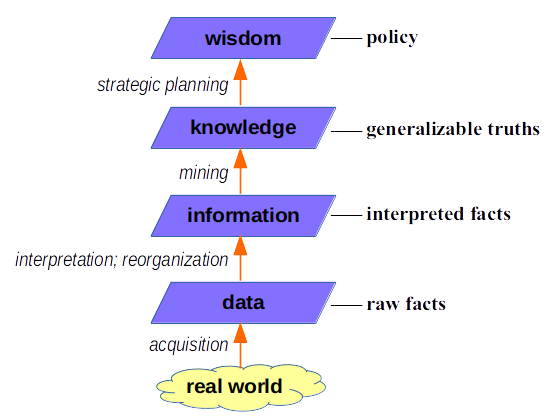
\includegraphics[width=0.9\textwidth]{dataHierarchy.png}
\caption{The data-to-wisdom hierarchy.}
\label{dataHierarchy}
\end{figure}

\subsection{The real world}
\index{real world}
\index{acquisition}

Ultimately, what we're interested in is not data, but aspects of the
\textbf{real world} -- album sales and video views, stock prices and employment
rates, hurricane trajectories and virus hot spots, or whatever. Data science
can't really get off the ground until some sort of \textbf{data acquisition}
takes place that records measurements of the real world in electronic form.

This sounds obvious, but it's important to keep in mind, actually. No matter
how much time we spend working with data, \textit{it's never the data that
actually matters -- it's the real-world phenomenon the data represents.} It
might seem strange to say that ``data'' is merely incidental to a data
scientist, but it's true. And I've definitely seen more than one data scientist
get so locked on to the data that they forget this basic truth.

One important observation is that decisions about exactly \textit{which} data
to acquire from the real world are often crucial in how things are interpreted
later on. To take an example close to home, let's say we're gathering
information on college professors so we can gauge which universities have the
highest performing faculty, and how this might be changing over the years. We
choose some representative set of criteria to measure for each faculty member
to get a rough assessment of their performance. Let's say we choose three
things: the number of research papers the professor publishes each year, the
total amount of research funding they've been granted, and the average student
evaluation score of the courses they teach. That seems like a good first cut at
assessing ``faculty performance.'' We then go on our merry data science way,
finding correlations, making data visualizations, and drawing conclusions.

This is all fine and dandy, provided we always keep in mind that it was those
three qualities, and \textit{only} those three, that we gathered in the first
place. If our study gains any traction, and university professors find they
have a vested interest in being ranked high in our yearly study, we'll discover
that they act to maximize \textit{only} the categories that are being
collected. We didn't gather data on how many university committees they served
on, or how many independent studies they supervised, or how many advisees they
had, \textit{etc.} Those metrics will inevitably become minimized in
importance, because they weren't part of what we lifted out of the real world
and onto the bottom rung of our lofty chain.

\index{GDP}
\index{Dow Jones Industrial Average}
\index{stock market}

The moral is: what we measure matters, often more than we realize. Our
country's GDP and the Dow Jones Industrial Average are easy things to quantify,
and so we often do. And thus they gain great importance in analyses of the
economy. But are they actually the most important indicators? Does focusing on
them leave out other, perhaps more vital, benchmarks? I'll just leave you with
that question for now.

\subsection{Data}

\index{gobbledy-gook}
\index{data}
\index{interpretation}

Have you ever gotten blood work done, say for an annual physical? I have. I
like to look over the numbers when the doctor hands me the results, just to
chuckle and wonder what they all mean. To me, a non-physician, they're all
pretty much gobbledy-gook. They tell me my TBC is 4.93 x10E6/$\mu$L, that
I have 5.7 Absolute Neutrophils, and a slightly out-of-range NT-proBNP (just
53.49 pg/mL, whatever the heck that means).

When I use the word \textbf{data} in the context of the hierarchy, this is what
I mean: recorded measurements, often (but not always) quantitative, that have
not yet been \textbf{interpreted}. They may be very precise, but they're also
quite meaningless without the context in which to understand them. They'd even
be meaningless to a \textit{physician} if I didn't provide the labels; try
telling your doctor that you have 4.93 ``something'' and see whether he/she
freaks out.

The good news is that when we're at the data stage of the hierarchy, we at
least have the stuff in an electronic form so we can start to \textit{do}
something with it. We also often make choices at this stage about how to
\textbf{organize} the data, choosing the appropriate type of atomic and/or
aggregate data structures that we'll discuss in detail in
Chapters~\ref{ch:atomicData} and beyond. This will allow us to bring our
analysis equipment to bear on the problem in powerful ways.

\subsection{Information}
\index{information}

Data becomes \textbf{information} when it \textit{informs} us of something;
\textit{i.e.}, when we know what it means. Getting large amounts of data
organized, formatted, and labeled the right way are jobs for the data
scientist, since turning that morass into useful knowledge is impossible
without those steps. When the aspects of the real world that we've collected
are properly structured and conceptually meaningful, we're in business.


\subsection{Knowledge}
\index{knowledge}
\index{generalizable truths}

Now \textbf{knowledge} is where the real action is. As shown in
Figure~\ref{dataHierarchy}, knowledge consists of \textit{generalizable}
truths.

\index{Chandra}
\index{Austin}
\index{bank teller}

Here's what I mean. Information is about specific individuals or occurrences.
When we say ``Chandra is a female bank teller, and earns \$48,000 a year,'' or
``Austin is a male bank teller, and earns \$69,000 a year,'' we have in our
information repository some individual facts. They can be looked up and
consulted when necessary, as you'll learn in the first part of this book.

But if we say ``women make less money than men do, even at the same jobs,''
we're in a different realm entirely. We have now generalized from specific
facts to more wide-reaching tendencies. In the language of our discipline,
we've moved from information to knowledge.

Properly gleaning knowledge from information is a trickier business than
interpreting individual data points. There are established rules, some of them
mathematical, for determining when an apparent pattern is actually reliable,
what kinds of relationships can be detected with data, whether a relationship
is causal, and so forth. We'll build some important foundations with this kind
of reasoning in this \textit{Crystal Ball} volume and its follow-on companion.
For now, I only want to make the point that \textit{knowledge} -- as opposed to
mere information -- opens up a whole new world of understanding. No longer is
the world limited to a chaotic collection of individual observations: we can
now begin to understand the general ways in which the world works...and perhaps
even to change them.

\subsection{Wisdom}
\index{wisdom}

\textbf{Wisdom} is the gold standard. It represents what we \textit{do} with
our knowledge. Let's say we indeed determine that on average men are paid
higher than women in our country, even for the same jobs. What do we do with
that realization? Is it okay? Do we want to try and fix it, and if so, how?
With laws? Education? Government subsidies? Revolution?

\index{simulation}
\index{uncertainty}

You'll remember my definition of Data Science on p.~\pageref{dsDefinition}:
deriving \textit{knowledge} from \textit{data}. This implies that the
``wisdom'' level of the hierarchy is really outside the discipline, and belongs
to other disciplines instead. And that's partially true: in some sense, the
data scientist's job stops when the deep truths about the real world are
ferreted out and illustrated, leaving it to CEOs, directors, and other policy
makers to act on them. But the data scientist is often involved here too, for a
simple reason: a decision maker wants to know what's likely to \textit{happen}
if a particular policy is implemented. Most non-trivial interventions will have
results that are hard to predict in advance, as well as unintended side
effects. One set of tools in the data scientist's toolkit is for making
principled, calculated predictions about such things, as well as quantifying
the level of \textbf{uncertainty} in the predictions. Sometimes, the technique
of \textbf{simulation} is used -- carrying out experiments on virtual societies
or systems to see the likely aggregate effects of different interventions. It's
like having a high-dimensional, multi-faceted crystal ball that lets you play
out various scenarios to their logical conclusions.

\bigskip

Starting with the rough and tumble real world and helping produce wise
decisions about how humankind can deal with it all: that's the grand promise of
the data science enterprise. And those are the mighty waters you're about to
dip your toes in! I hope you'll find it as exhilarating as I do.

% TODO: Applications (sports, Netflix, image recognition, Google, NLP,
% Coronavirus)


\section{A word of warning}

\index{Spiderman}

Before we dive into the nitty gritty, let me leave you with one more general
thought. It's actually an application of something Spiderman once said: ``with
great power comes great responsibility.''

\index{walking on water}

Here's the deal. The skills you'll learn in this book are so powerful and
(still!) so rare, that when you demonstrate them, people will think you can
walk on water. If you continue in the discipline, you'll become highly
sought-after (and well paid). People will constantly be asking you to work
with new data, to produce plots, predictions, and insights, and basically to do
your magic. You'll be treated as a guru: the oracle people go to when they want
the scoop.

This is ultra-cool, but also dangerous. Why dangerous? One simple reason:
because \textit{when you make a data-related claim, \textbf{people will believe
you.}} Pretty much unquestioningly. Most of your colleagues won't have the
expertise or understanding to double-check your snazzy results. And it wouldn't
occur to them to do that anyway -- after all, you're the wizard.

\index{uncertainty}

The truth of the matter is that data science lives on the knife edge of
\textbf{uncertainty}. With our crystal ball, we can make non-obvious assertions
about the past or present and even predict the future, but as with all
``knowledge,'' we must always hold it tentatively. We may be 95\% confident
that men are paid more than women...but that's only 95\% confidence, not 100\%.
We may have reason to believe that raising the minimum wage in a city will
decrease poverty by 3\%...but there's a 1 in 20 chance that it might decrease
it by as much as 6\%, or even \textit{increase} it by 1\%.

The abiding principle is that you should always be forthright about the limits
of your bold claims, the caveats behind your beautiful plots, and the level of
likelihood that your hypotheses will turn out to be wrong. Admittedly, doing so
will make you seem a little less magic. There are lots of talking heads on
television who deliberately \textit{obscure} the level of uncertainty in their
analyses so that they seem more certain (and more impressive) than they really
are. To be responsible data scientists, though, we're going to do the Spiderman
thing and be up front and transparent about exactly what we've found, and what
we might be missing.

Believe me, this will make you powerful enough!


\chapter{A trip to Jupyter}

\label{programmingEnvironment}
\index{execute}
\index{edit}
\index{language}
\index{environment!programming}
\index{programming environment}
Python is a ridiculously popular \textbf{language} for programming and data
science (currently the third most widely used in the world\footnote{See
\url{https://www.tiobe.com/tiobe-index/}.}) which is one of many reasons we're
using it for this course. The language itself is different from the
\textbf{programming environment} used to write code in it, just as ``English''
is different from ``Microsoft Word'' and ``Google Docs.'' A programming
environment is just a fancy name for a tool or application used to write
programs. At a minimum, it must include a way to \textbf{edit} (write and
revise) code, and a way to \textbf{execute} (run) it.

\index{Jupyter Notebooks}
\index{IDE}
\index{Spyder}
There are many different programming environments data scientists use to write
Python code, just as there are many different word processing apps people use
to write English. The choice largely comes down to personal preference. Some
use full-blown \textbf{IDE}s (``integrated development environments'') like
Spyder or Atom; some use text-based tools like Notepad++ or \texttt{vim}. In
this class, we're going to use the friendly and minimalistic ``\textbf{Jupyter
Notebooks}'' environment since it's appropriate for an intro experience.

\section{Jupyter Notebooks}

\index{cell}

The concept of a Jupyter Notebook is simple: it's a Web page with editable
``\textbf{cell}s.'' Each cell is a little text window you can type in.

\pagebreak
There are three kinds of cells in Jupyter Notebooks:
\vspace{-.15in}

\begin{description}
\index{cell!raw}
\item{\textbf{Raw.}} ``Raw'' is dumb. Never use it.
\index{Markdown}
\index{render}
\index{cell!Markdown}
\item{\textbf{Markdown.}} ``Markdown'' cells are for \textit{English text}, not Python
code. They're mostly used to describe and annotate what you're doing in the
code cells, like a running commentary. You can type plain-ol' text in a
Markdown cell, plus various cutesy formatting adornments like boldface (putting
double-splats (\texttt{**}) around a word or phrase), italics (single splats),
outline headings (prefacing a line with one or more hashtags (like \texttt{\#}
or \texttt{\#\#\#}), and so forth.\footnote{For a complete list of formatting
options, see
\url{https://github.com/adam-p/markdown-here/wiki/Markdown-Cheatsheet}.} When
you type in a Markdown cell, you see the raw text and formatting; to actually get Jupyter to
\textbf{render} your cells and make them pretty, you choose ``Run All'' from
the \index{run all@``Run All''} \index{cell menu@``Cell'' CoCalc menu} ``Cell'' menu.

\index{cell!Code}
\item{\textbf{Code.}} The most important cells are ``Code'' cells which contain (duh)
code. When executed (again, by choosing ``Run All'' from the ``Cell'' menu) they actually carry out
the Python instructions you have typed in that cell, and display any results.

\end{description}

By the way, a common snafu is to somehow accidentally click in a way that
changes the type of a cell from ``Code'' to one of the other types. If you do
this, the Python code in that cell won't execute until you change the type back
to ``Code'' (more on this below).

\index{cell!type dropdown}
\index{CoCalc}
Figure~\ref{fig:jupyterNotebook} shows a Jupyter Notebook hosted by the
\textbf{CoCalc} cloud computing platform, which we'll use this semester. It has
two cells, one Markdown and one Code. Note carefully the \textbf{cell-type
dropdown} which is kind of hidden in the middle of the page: it currently reads
``Code'' because the second cell is the one that's highlighted. (If we clicked
to highlight and edit the top cell, that dropdown would change to
``Markdown.'')

\begin{figure}[!h]
\centering
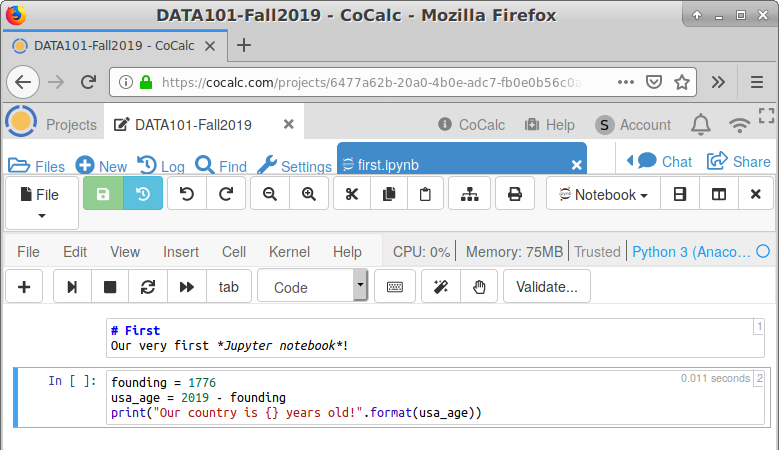
\includegraphics[width=0.85\textwidth]{firstNotebook.png} \\
\bigskip
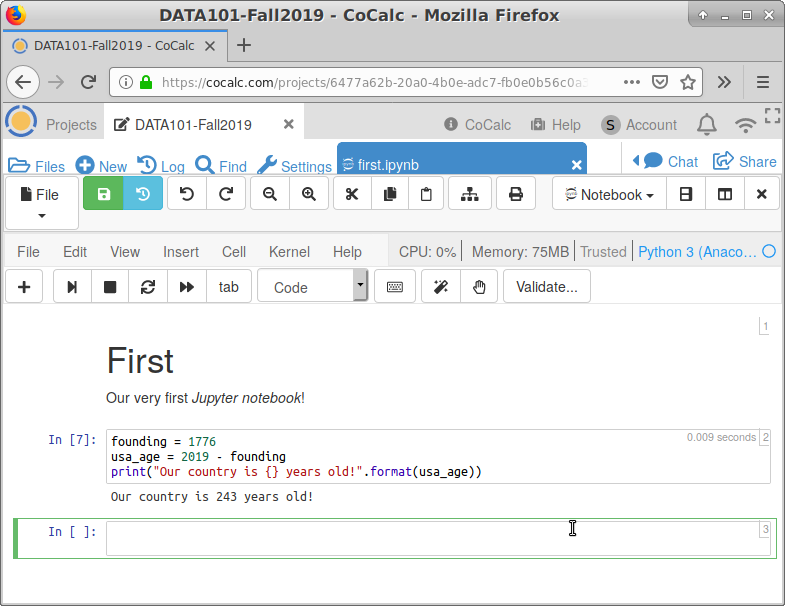
\includegraphics[width=0.85\textwidth]{firstNotebook2.png}
\medskip
\caption{A Jupyter Notebook with one Markdown cell and one Code cell. In the
top image, the two cells have been edited but not yet ``run'' -- hence
the Markdown formatting is unrendered and the code has not been executed. The
bottom pane shows both cells after the use has chosen ``Run All'' from the
``Cell'' menu.}
\label{fig:jupyterNotebook}
\end{figure}

\index{code snippet}
\index{snippet}
\index{output}
\index{*@\texttt{*} (splat)}
\index{splat}

The top figure shows the two cells before the user has done a ``Run All'' from
the ``Cell'' menu: all\index{run all@``Run All''} \index{cell menu@``Cell''
CoCalc menu} the Markdown is unrendered (see the literal splats and hashtags)
and the code is just sitting there. After ``Run All,'' the picture changes: you
see the formatted message in the top cell, and the \textbf{output} of the
Python code snippet after it runs. (The latter is easy to miss; stare at that
bottom picture and find the ``\texttt{Our country is 245 years old!}'' message.
That's the ``output.'') We haven't yet covered what that Python code means
(that's the main subject of this book) but you can probably guess some of what
it's doing.

%(Incidentally, you can see that when you Shift-Enter the bottom cell to run the
%code, Jupyter also creates a new empty cell at the end of the Notebook for you
%to type in. I find this annoying, but whatever.)

\section{Code and output}

Incredibly, that's about it. Everything else in this book is going to concern
what to type in those Code cells and how to interpret its output.

From now on, whenever I give example Python code in this book, I'll write it in
a box like this:

\begin{Verbatim}[fontsize=\small,samepage=true,frame=single,framesep=3mm]
founding = 1776
usa_age = 2021 - founding
print("Our country is {} years old!".format(usa_age))
\end{Verbatim}

That box means ``this stuff goes in a Code cell of a Notebook.''

When I write the corresponding output (\textit{i.e.}, what gets printed on the
page immediately below the code cell when ``Run All'' is chosen from the
``Cell'' menu), I'll write it like this:
\index{run all@``Run All''} \index{cell menu@``Cell'' CoCalc menu} 
\begin{Verbatim}[fontsize=\small,samepage=true,frame=leftline,framesep=5mm,framerule=1mm]
Our country is 245 years old!
\end{Verbatim}

That vertical bar means ``this stuff is the printed result of executing the
code cell.''

Easy enough. Onward!


% Other stuff I mentioned in class:
%
% For math, you think holistically. For programming, you think sequentially /
%   algorithmically.

\chapter{Three kinds of atomic data}
\label{ch:atomicData}

\section{Atomic data}

\index{atomic}
\index{indivisible}
When we say that some data is ``\textbf{atomic},'' we don't mean it's
radioactive; we mean it's \textit{indivisible}.

\index{Democritus}
\index{apple}
The ancients spoke of ``atoms'' as the smallest possible bits of matter. If you
divide up any physical object -- say, an apple -- into parts, you get its
components: a stalk, a stem, skin, seeds, and the sweet juicy stuff. Cut up any
of \textit{those} pieces with a knife and you get smaller pieces. If you
continue to split and split and split, philosophers like Democritus reasoned,
you'll eventually get to tiny indivisible bits that cannot be further
dissected. This is where the physical world bottoms out at the finest degree of
granularity.

Similarly, a piece of atomic data is typically treated as an entire unit, not
as something with internal structure that can be broken down. In the next
chapter we'll learn about various ways that these atoms of data can be strung
together and organized into larger wholes; for now, though, we're just looking
at the atoms themselves.

\section{Environments and variables}

\label{sec:envsAndVariables}
\index{environment}
\index{variable}
\index{variable!name}
\index{variable!value}
A data analysis program -- of which we will write many in this course -- makes
use of an \textbf{environment} as it runs. ``Environment'' just means ``all the
data that is currently in view, and which the program can
access.''\footnote{Confusingly, this use of the term ``environment'' is
different from the term ``programming environment'' I introduced on
p.\pageref{programmingEnvironment}.}  The environment consists of
\textbf{variables}, each of which (usually) has a \textbf{name} and a
\textbf{value}. For example, we might have a variable named \texttt{age} whose
value is 21, and a variable named \texttt{slogan} whose value is
\texttt{"Finger lickin' good"}.

\index{variable!name}
Each variable in the environment must have a \textit{distinct} name
(\textit{i.e.}, no two variables can share the same name). Also, importantly,
the reason these building blocks are called ``variables'' is that their value
can \textit{change} as the program executes. Although we may initially create
an \texttt{age} variable with the value \texttt{21}, later on in the program
the variable's value might change to \texttt{22}, or \texttt{50}, or
\texttt{0}. The variable's \textit{name} never changes, though.

\section{Atomic data types}

\index{variable!type}
There's one other thing that a variable has in addition to its name and value:
a \textbf{type}.\footnote{Strictly speaking, although in languages like Java
variables indeed have types, in Python the \textit{values} have types, not the
variables. This distinction will never be important for us though.}  In a
programming language like Python, every piece of data has a specific type,
which is necessary for determining how it behaves and what all you can do to
it. A question you should ask yourself a lot is: ``okay, I've got a variable in
my environment called \texttt{x}...now what is its type?'' You might have
guessed (correctly) that our \texttt{age} and \texttt{slogan} variables from
the previous section are of different types: one is a number, and the other is
a phrase.

In this course, we'll principally deal with three types of atomic data, all of
which will be familiar to you.


\subsection{Whole numbers}

\index{variable!whole number}
\index{whole number}
\index{likes@``likes''}
\index{votes}
One very common type of data is whole numbers, or integers. These are usually
positive, but can be negative, and have no decimal point. Things like a
person's birth year, a candidate's vote total, or a social media post's number
of ``likes'' are represented with this data type.


\subsection{Real (fractional) numbers}

\index{variable!real number}
\index{real number}
\index{fractional number}
\index{Facebook}
\index{movie rating}
\index{interest rate}
\index{temperature}
You may remember from high school math that the so-called ``real numbers''
include not only integers, but also numbers with digits after the decimal
point. This type can therefore be used to store interest rates, temperature
readings, and average movie ratings on a 1-to-5 scale.

Since all whole numbers are themselves real numbers, you might wonder why we
bother to define two different types for these. Why not just give both kinds of
variables the same real number type? Basically, the answer is that something
``feels wrong'' about that to the Data Science community. A Facebook user might
have 240 friends, or 241, but it would never make sense for her to have 240.3
friends. A consensus has thus arisen: variables that would only ever store
whole numbers really ought to be of a type that's devoted to only whole
numbers. You can violate this convention, but you'll be thought weird by your
fellow developers if you do so.


\subsection{Text}

\index{text}
\index{variable!text}
Lastly, some values obviously aren't numeric at all, like a customer's name, a
show title, or a tweet. So our third type of data is textual. Variables of this
type have a sequence of characters as values. These characters are most often
English letters, but can also include spaces, punctuation, and characters from
other alphabets.

\index{atomic}
\index{Avengers: Endgame@\textit{Avengers: Endgame}}
By the way, this third data type can tiptoe right up to the ``atomic'' line and
sometimes cross it. In other words, we will occasionally work with text values
\textit{non}-atomically, by splitting them up into their constituent words or
even letters. Most of the time, though, we'll treat a character sequence like
\texttt{"Avengers:\ Endgame"} as a single, indivisible chunk of data in the
same way we treat a number like \texttt{42}.

\subsection{But what about...?}

\index{song file}
\index{image file}
\index{video file}
What about other things a computer can store: images, song files, videos? It
turns out that through clever tricks, all these kinds of media and more can be
boiled down to a large number of integers, and stored in an aggregate data
structure like those discussed in the next chapter. At the atomic level, we'll
really only ever need to deal with the three types of this section.

\section{The three kinds in Python}

\index{language-general}
Now the three kinds of atomic data described above are
\textbf{language-general}: this means that they're conceptual, not tied to any
specific programming language or analysis tool. \textit{Any} technology used
for Data Science will have the ability to deal with those three basic types.
The specific ways they do so will differ somewhat from language to language.
Let's learn about how Python implements them.

\subsection{Whole numbers: \texttt{int}}

\index{int@\texttt{int}}
\index{integer}
One of the most basic Python data types is the ``\texttt{int},'' which stands
for ``integer.'' It's what we use to represent whole numbers.

\index{variable!value}
In Python, you create a variable by simply typing its name, an equals sign, and
then its initial value, like so:

\begin{Verbatim}[fontsize=\small,samepage=true,frame=single,framesep=3mm]
revolution = 1776
\end{Verbatim}

\index{line of code}
\index{code}
\index{executing@executing (code)}
\index{statement}
This is our first \textbf{line of code}\footnote{By the way, the word
\textbf{code} is grammatically a mass noun, not a count noun. Hence it is
proper to say ``I wrote some code last night,'' not ``I wrote some codes last
night.'' If you misuse this, it will brand you as a newbie right away.}. As
we'll see, lines of code are \textbf{executed} one by one -- there is a time
before, and a time after, each line is actually carried out. This will turn out
to be very important. (Oh, and a ``line of code'' is sometimes also called a
\textbf{statement}.)


\index{variable!name}
\index{underscore}
Python variable names can be as long as you like, provided they consist only of
upper and lower case letters, digits, and underscores. (You do have to be
consistent with your capitalization and your spelling: you can't call a
variable \texttt{Movie} in one line of code and \texttt{movie} in another.)
Underscores are often used as pseudo-spaces, but no other weird punctuation
marks are allowed in a variable's name.\footnote{Oh, and another rule: a
variable name can't \textit{start} with a digit. So \texttt{r2d2} is a legal
variable name, but not \texttt{007bond}.}

\index{movie rating}
\index{revolution@\texttt{revolution}}
And while we're on the subject, let me encourage you to \textit{name your
variables well}. This means that each variable name should reflect
\textit{exactly} what the value that it stores represents. Example: if a
variable is meant to store the rating (in ``stars'') that an IMDB user gave to
a movie, don't name it \texttt{movie}. Name it \texttt{rating}. (Or even
better, \texttt{movie\_rating}.) Trust me: when you're working on a complex
program, there's enough hard stuff to think about without confusing yourself
(and your colleagues) by close-but-not-exact variable names.\footnote{And I
fully own up to the fact that the \texttt{revolution} variable isn't named very
well. I chose it to make a different point shortly.}

\index{variable!type}
Now remember that a variable has three things -- a name, value, and type. The
first two explicitly appear in the line of code itself. As for the type, how
does Python know that \texttt{revolution} should be an ``\texttt{int}?''
Simple: it's \textit{a number with no decimal point.}

As a sanity check, we can ask Python to tell us the variable's type explicitly,
by writing this code:

\index{type@\texttt{type()}}
\label{typeFunction}
\begin{Verbatim}[fontsize=\small,samepage=true,frame=single,framesep=3mm]
type(revolution)
\end{Verbatim}

If this line of code is executed after the previous one is executed, Python
responds with:

\begin{Verbatim}[fontsize=\small,samepage=true,frame=leftline,framesep=5mm,framerule=1mm]
int
\end{Verbatim}

So there you go.

\index{code snippet}
\index{snippet}
Here's another ``\textbf{code snippet}'' (a term that just means ``some lines
of code I'm focusing on, which are generally only part of a larger program''):

\begin{Verbatim}[fontsize=\small,samepage=true,frame=single,framesep=3mm]
revolution = 1776
moon_landing = 1969
revolution = 1917
\end{Verbatim}

\index{revolution@\texttt{revolution}}
Now if this were a math class, that set of equations would be nonsensical. How
could the same variable (\texttt{revolution}) have two contradictory values?
But in a \textit{program}, this is perfectly legit: it just means that
immediately after the first line of code executes, \texttt{revolution} has the
value \texttt{1776}, and moments later, after the third line executes, its
value has changed to \texttt{1917}. Its value depends entirely on ``where the
program is'' during its execution.

\subsection{Real (fractional) numbers: \texttt{float}}

\index{float@\texttt{float}}
The only odd thing about the second data type in Python is its name. In some
other universe it might have been called a ``real'' or a ``decimal'' or a
``fractional'' variable, but for some bizarre historical reasons it is called a
\texttt{float}.\footnote{If you're curious, this is because in computer
programming parlance a ``floating-point number'' means a number where the
decimal point might be anywhere. With an integer like -52, the decimal point is
implicitly at the far right-hand side of the string of digits. But with numbers
like -5.2 or -.52 or -.000052 or even 520000, the decimal point has ``floated''
away from this fixed position.}

\index{decimal point}
All the same rules and regulations pertain to \texttt{float}s as they do to
\texttt{int}s; the only difference is you type a decimal point. So:

\begin{Verbatim}[fontsize=\small,samepage=true,frame=single,framesep=3mm]
GPA = 3.17
price_of_Christian_Louboutin_shoes = 895.95
interest_rate = 6.
\end{Verbatim}

\index{interest rate}
Note that the \texttt{interest\_rate} variable is indeed a \texttt{float} type
(even though it has no fractional part) because we typed a period:

\index{type@\texttt{type()}}
\begin{Verbatim}[fontsize=\small,samepage=true,frame=single,framesep=3mm]
type(interest_rate)
\end{Verbatim}
\begin{Verbatim}[fontsize=\small,samepage=true,frame=leftline,framesep=5mm,framerule=1mm]
float
\end{Verbatim}

\subsection{Text: \texttt{str}}

\index{string}
\index{str@\texttt{str}}
Speaking of weird names, a Python text variable is of type \texttt{str}, which
stands for ``\textbf{string}.'' You could think of it as a bunch of letters
``strung'' together like a beaded necklace.

\index{quotation marks}
\index{''@\texttt{\textquotesingle\textquotesingle} (ticks)}
\index{""@\texttt{\char`\"\char`\"} (quotes)}
Important: when specifying a \texttt{str} value, you must use \textbf{quotation
marks} (either single or double). For one thing, this is how Python tells that
you intend to create a \texttt{str} as opposed to some other type. Examples:

\index{lit}
\index{donut\_store@\texttt{donut\_store}}
\index{Paul's Bakery}
\begin{Verbatim}[fontsize=\small,samepage=true,frame=single,framesep=3mm]
slang = 'lit'
grade = "3rd"
donut_store = "Paul's Bakery"
url = 'http://umweagles.com'
\end{Verbatim}

\index{string!of digits}
\index{type@\texttt{type()}}
Notice, by the way, that a \textit{string of digits} is not the same as an
integer. To wit:

\begin{Verbatim}[fontsize=\small,samepage=true,frame=single,framesep=3mm]
schwarzenegger_weight = 249
action_movie = "300"

type(schwarzenegger_weight)
\end{Verbatim}
\begin{Verbatim}[fontsize=\small,samepage=true,frame=leftline,framesep=5mm,framerule=1mm]
int
\end{Verbatim}

\begin{Verbatim}[fontsize=\small,samepage=true,frame=single,framesep=3mm]
type(action_movie)
\end{Verbatim}
\begin{Verbatim}[fontsize=\small,samepage=true,frame=leftline,framesep=5mm,framerule=1mm]
str
\end{Verbatim}

See? The quotes make all the difference.

\subsubsection{The length of a string}

\index{string!length}
\index{len@\texttt{len()}}
We'll do many things with strings in this book. Probably the most basic is
simply to inquire as to a string's \textbf{length}, or the number of characters
it contains. To do this, we enclose the variable's name in parentheses after
the word \texttt{len}:

\begin{Verbatim}[fontsize=\small,samepage=true,frame=single,framesep=3mm]
len(slang)
\end{Verbatim}
\begin{Verbatim}[fontsize=\small,samepage=true,frame=leftline,framesep=5mm,framerule=1mm]
3
\end{Verbatim}

\begin{Verbatim}[fontsize=\small,samepage=true,frame=single,framesep=3mm]
len(donut_store)
\end{Verbatim}
\begin{Verbatim}[fontsize=\small,samepage=true,frame=leftline,framesep=5mm,framerule=1mm]
13
\end{Verbatim}

\label{function}
\index{lingo}
\index{function}
\index{argument}
\index{calling a function@``calling'' a function}
As we'll see, the \texttt{len()} operation (and many others like it) is an
example of a \textbf{function} in Python. In proper lingo, when we write a line
of code like \texttt{len(donut\_store)} we say we are ``\textbf{calling the
function},'' which simply means to invoke or trigger it.

\index{pass}
\index{passing an argument@``passing'' an argument}
\index{bananas (parentheses)}
\index{()@\texttt{()} (bananas)}
More lingo: for obscure reasons, the value inside the bananas
(here, \texttt{donut\_store}) is called an \textbf{argument} to the
function. And we say that we ``\textbf{pass}'' one or more arguments to a
function when we call it.

All these terms may seem pedantic, but they are precise and universally-used,
so be sure to learn them. The preceding line of code can be completely summed
up by saying:

\begin{quote}
``We are \textbf{calling} the \texttt{len()} \textbf{function},
and \textbf{passing} it the \texttt{donut\_store} \textbf{variable} as an
\textbf{argument}.''
\end{quote}

I recommend you say that sentence out loud at least four times in a row to get
used to its rhythm.

Note, by the way, that the \texttt{len()} function expects a \texttt{str}
argument. You can't call \texttt{len()} with an \texttt{int} or a
\texttt{float} variable as an argument:

\begin{Verbatim}[fontsize=\small,samepage=true,frame=single,framesep=3mm]
schwarzenegger_weight = 249

len(schwarzenegger_weight)
\end{Verbatim}

\begin{Verbatim}[fontsize=\small,samepage=true,frame=leftline,framesep=5mm,framerule=1mm]
TypeError: object of type 'int' has no len()
\end{Verbatim}

(You might think that the ``length'' of an \texttt{int} would be its number of
digits, but nope.)

\index{variable}
\index{variable!value}
One thing that students often get confused is the difference between a named
string \textit{variable} and that of an (unnamed) string \textit{value}.
Consider the difference in outputs of the following:

\begin{Verbatim}[fontsize=\small,samepage=true,frame=single,framesep=3mm]
slang = 'lit'
len(slang)
\end{Verbatim}
\begin{Verbatim}[fontsize=\small,samepage=true,frame=leftline,framesep=5mm,framerule=1mm]
3
\end{Verbatim}
\begin{Verbatim}[fontsize=\small,samepage=true,frame=single,framesep=3mm]
len('slang')
\end{Verbatim}
\begin{Verbatim}[fontsize=\small,samepage=true,frame=leftline,framesep=5mm,framerule=1mm]
5
\end{Verbatim}

In the first example, we asked ``how long is the value being held in the
\texttt{slang} variable?'' The answer was 3, since ``\texttt{lit}'' is three
characters long. In the second example, we asked ``how long is the word
\texttt{\textquotesingle slang\textquotesingle}?'' and the answer is 5. Remember: variable names never go in
quotes. If something is in quotes, it's being taken \textit{literally}.


\subsection{Combining and printing variables}

\index{printing a variable}
\index{print@\texttt{print()}}
There's a whole lot of stuff you can do with variables other than just creating
them. One thing you'll want to do frequently is \textbf{print} a variable,
which means to dump its value to the page so you can see it. This is easily
done by calling the \texttt{print()} function:

\begin{Verbatim}[fontsize=\small,samepage=true,frame=single,framesep=3mm]
print(donut_store)
print(price_of_Christian_Louboutin_shoes)
print("slang")
print(slang)
\end{Verbatim}

\begin{Verbatim}[fontsize=\small,samepage=true,frame=leftline,framesep=5mm,framerule=1mm]
Paul's Bakery
895.95
slang
lit
\end{Verbatim}

Again, don't miss the crucial difference between printing \texttt{"slang"} and
printing \texttt{slang}. The former is literal and the latter is not. In the
first of these, we're passing the \textit{word} ``\texttt{slang}'' as the
argument, not the variable \texttt{slang}.

\index{method}
Often we'll want to combine bits of information into a single print statement.
Typically one of the variables is a string that contains the overall message.
There are several ways to accomplish this, but the most flexible will turn out
to be the \texttt{.format()} \textbf{method}.

\index{calling a method@``calling'' a method (on a variable)}
\index{on@``on''}
I hate to hit you with so much new lingo. A \textbf{method} is very similar to
a function, but not exactly. The difference is in the syntax used to call it.
When you call a function (like \texttt{type()} or \texttt{len()}) you simply
type its name, followed by a pair of bananas inside of which you put the
arguments (separated by commas, if there's more than one). But when you ``call
a method,'' you put \textit{a variable} before a dot (``\texttt{.}'') and the
method name, then the bananas. This is referred to as ``calling the method
\textbf{on} the variable.''

It sounds more confusing than it is. Here's an example of \texttt{.format()} in
action:

\begin{Verbatim}[fontsize=\small,samepage=true,frame=single,framesep=3mm]
price_of_Christian_Louboutin_shoes = 895.95
message = "Honey, I spent ${} today!"
print(message.format(price_of_Christian_Louboutin_shoes))
\end{Verbatim}

\index{matching bananas}
\index{double bananas@``double bananas''}
Take note of how we write ``\texttt{message.format}'' instead of just
``\texttt{format}''. This is because \texttt{.format()} is a method, not a
function. We say that we are calling \texttt{.format()} ``on''
\texttt{message}, and passing \texttt{price\_of\_}\ \texttt{Christian\_Louboutin\_shoes}
as an argument.\footnote{Btw, in this book, whenever I refer to a method, I'll
be sure to put a dot before its name. For example, it's not the
``\texttt{format()}'' method, but the ``\texttt{.format()}'' method.} Also be
sure to notice the \textit{double} bananas ``\texttt{))}'' at the end of that
last line. We need both of them because in programming, every left-banana must
match a corresponding right-banana. Since we're calling two functions/methods
on one line (\texttt{print()} and \texttt{.format()}), we had two left-bananas
on that line. Each one needs a partner.

\index{\{\}@\texttt{\{\}} (curlies)}
As for the specifics of how \texttt{.format()} works, you'll see that the
string variable you call it on may include pairs of curlies (squiggly braces).
These are placeholders for where to stick the values of other variables in the
output. Those variables are then included as arguments to the
\texttt{.format()} method. The above code produces this output:

\begin{Verbatim}[fontsize=\small,samepage=true,frame=leftline,framesep=5mm,framerule=1mm]
Honey, I spent $895.95 today!
\end{Verbatim}

Often, instead of creating a new variable name to hold the pre-formatted
string, we'll just \texttt{print()} it literally, like this:

\begin{Verbatim}[fontsize=\footnotesize,samepage=true,frame=single,framesep=3mm]
print("Honey, I spent ${} today!".format(
    price_of_Christian_Louboutin_shoes))
\end{Verbatim}

We're still actually calling \texttt{.format()} on a variable here, it's just
that we haven't bothered to name the variable. Also, notice that our code was
too long to fit on one line nicely, so we broke it in two, and indented the
second line to make it clear that ``\texttt{price\_of\_}...'' wasn't
starting\index{bananas (parentheses)}\index{()@\texttt{()} (bananas)} its own new
line. Crucially, all the bananas are still paired up, two-by-two, even though
the left bananas are on a different line than the corresponding right bananas.

\bigskip
Finally, here's a longer example with more variables:

\begin{Verbatim}[fontsize=\footnotesize,samepage=true,frame=single,framesep=3mm]
name = "Pedro Pascal"
num_items = 3
cost = 91.73
print("Customer {} bought {} items worth ${}.".format(name,
    num_items, cost))
\end{Verbatim}

\begin{Verbatim}[fontsize=\small,samepage=true,frame=leftline,framesep=5mm,framerule=1mm]
Customer Pedro Pascal bought 3 items worth $91.73.
\end{Verbatim}

You can see how we can pass more than one argument to a function/method simply
by separating them with commas inside the bananas.


% TODO:
%   pow() function
%   .strip() string method
% memory diagrams -- diff between modifying in place and returning a copy (like
% .strip().)
% Left-side "variable names and atomic data". Right-side "aggregate data."

\chapter{Memory pictures}

Now that we've talked about the three important kinds of atomic variables,
let's consider the question of \textit{where they live}. It might sound like a
strange question. Aren't they ``in'' the Jupyter Notebook cell in which they
were typed?

Actually, no. And that brings me to the first mission-critical lesson of the
semester, which is a bane to all students who don't deeply grasp it. The lesson
is:

\begin{quote}
\textbf{The code itself is only a means to an end. The purpose of the code is
to read or write what's in memory.}
\end{quote}

\index{memory}
\index{environment}
\textbf{Memory} is the part of the computer in which variables and their values
are stored. To use the terminology of Chapter~\ref{ch:atomicData}, memory is
where the \textbf{environment} lives. It is \textit{invisible} to the
programmer, but it is also \textit{very much there.} The single most important
trick to learning how to write correct code is being able to summon to mind
what memory looks like at any point in time. The code you must write is a
natural consequence of that.

\section{A picture of memory}

\index{memory!picture}
It's easier with pictures at first, so we'll draw plenty of them. Our
\textbf{memory pictures} will have a very specific format, and this is
crucially important: don't get creative with how things are labeled or where
things are drawn. In order for your code to work \textit{you must have this
picture exactly right.} It's not art; it's science.

Our memory pictures will always be divided into exactly two ``realms,'' one on
the left and one on the right, labeled as follows:

\begin{center}

\includegraphics[width=.7\textwidth]{memoryPicture.png}
\end{center}

The left column's name should be recognizable, since that's exactly what we
covered last chapter. The right column won't have anything in it for a couple
chapters.

\subsection{Writing to memory}

When we create atomic variables in a Code cell, a la:

\begin{Verbatim}[fontsize=\small,samepage=true,frame=single,framesep=3mm]
pin_count = 844
username = 'Bekka Palmer'
\end{Verbatim}

each one gets put on the left-hand side of the diagram as a \textbf{named box}.
The name of the box is the variable's name, and the thing inside of the box is
its value.

\vspace{-.2in}
\begin{center}
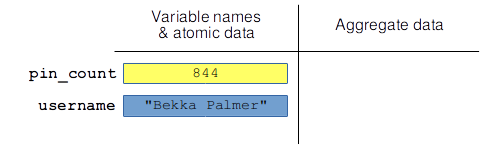
\includegraphics[width=.8\textwidth]{memoryPicture2.png}
\end{center}

It doesn't matter which boxes are higher or lower on the page, only that the
names stick with their boxes and don't get mixed up. As a bonus, I have colored
the boxes differently, indicating that \texttt{pin\_count} (an \texttt{int}) is
a different type than \texttt{username} (a \texttt{str}).\footnote{One other
tiny detail you might notice: even though our code had single quotes to delimit
Bekka Palmer's name, I put double quotes in the box in the memory picture. This
is to emphasize that no matter how you create a string in the code -- whether
with single quotes or double -- the underlying ``thing'' that gets written to
memory is the same. In fact, what's stored are actually the characters
\texttt{Bekka Palmer} \textit{without} the quotes. I like putting quotes in the
memory pictures, though, just to emphasize the string nature of the value.}

Creating more variables just adds more named boxes:

\begin{Verbatim}[fontsize=\small,samepage=true,frame=single,framesep=3mm]
...
avg_num_impressions = 1739.3
board_name = "Things to Make"
\end{Verbatim}

\vspace{-.2in}
\begin{center}
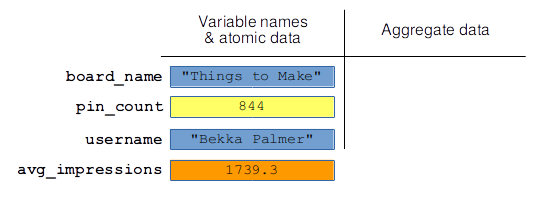
\includegraphics[width=.8\textwidth]{memoryPicture3.png}
\end{center}

I'm deliberately shuffling around the order of the boxes just to mess with you.
Python makes no guarantee of what ``order'' it will store variables in anyway,
and in reality it actually does become a big jumbled mess like this under the
hood. All Python guarantees is that it will consistently store a name, value,
and a type for each variable.

When we change the value of a variable (rather than creating a new one), the
value in the appropriate box gets updated:

\begin{Verbatim}[fontsize=\small,samepage=true,frame=single,framesep=3mm]
...
avg_num_impressions = 2000.97
pin_count = 845
another_board = 'Pink!'
\end{Verbatim}

\vspace{-.2in}
\begin{center}
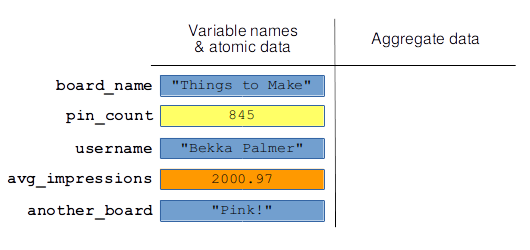
\includegraphics[width=.7\textwidth]{memoryPicture4.png}
\end{center}

Note carefully that \textit{the previous value in the box is completely
obliterated} and there is absolutely no way to ever get it back. There's no
way, in fact, to know that there even \textit{was} a previous value different
than the current one. Unless specifically orchestrated to do so, computer
programs only keep track of the present, not the past.

One other thing: unlike in some programming languages (so-called ``strongly
typed'' languages like Java or C++) even the \textit{type} of value that a
variable holds can change if you want it to. Even though the following example
doesn't make much sense, suppose we wrote this code next:

\begin{Verbatim}[fontsize=\small,samepage=true,frame=single,framesep=3mm]
...
pin_count = 999.635
username = 11
\end{Verbatim}

This causes not only the contents of the boxes to change, but even their
colors. The \texttt{username} variable was a \texttt{str} a moment ago, but now
it's an \texttt{int}.

\vspace{-.2in}
\begin{center}
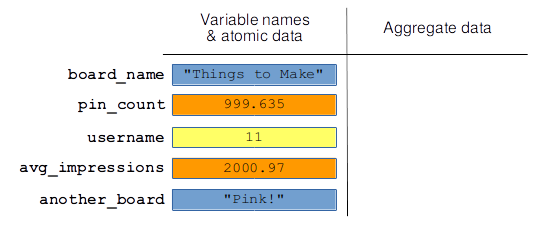
\includegraphics[width=.7\textwidth]{memoryPicture5.png}
\end{center}

\subsection{Reading from memory}

``Reading from memory'' just means referring to a variable in order to retrieve
its value. So far, we don't know how to do much with that other than print:

\begin{Verbatim}[fontsize=\small,samepage=true,frame=single,framesep=3mm]
print("The {} board has {} pins.".format(another_board, pin_count))
\end{Verbatim}

\begin{Verbatim}[fontsize=\small,samepage=true,frame=leftline,framesep=5mm,framerule=1mm]
The Pink! board has 999.635 pins.
\end{Verbatim}

The important point is that the memory picture is the (only) current, reliable
record of what memory looks like at any point in a program. Think of it as
reflecting a snapshot in time: immediately after some line of code executes --
and right before the following one does -- we can consult the picture to obtain
the value of each variable. This is exactly what Python does under the hood.

I stress this point because I've seen many students stare at complicated code
and try to ``think out'' what value each variable will have as it runs. That's
hard to do with anything more than a few lines. To keep track of
what-has-changed-to-what-and-when, you really need to maintain an up-to-date
list of each variable's value as the program executes...which is in fact
exactly what the memory picture is.

So if you're trying to figure out ``what will this program output if I print
the \texttt{odometer} variable immediately after line 12?'' don't stare at the
code and try to reconstruct its behavior from scratch. Instead, draw a memory
picture, update it accordingly as you walk through each line of code, and then
look at it for the answer.

\subsection{Tip}

By the way, investing in a small whiteboard and a couple of markers is a great
way to help you learn programming. They're perfect for drawing and updating
memory pictures as they evolve.

Hopefully this chapter was straightforward. These memory pictures will be
getting increasingly complex as we learn more kinds of things to store,
however, so stay sharp!


\chapter{Calculations}
\label{ch:calculations}

Our discipline obviously involves a lot of computation -- in fact, I expect the
first image that comes to mind when most people hear the words ``data science''
is one of numerical calculation. In this chapter, I'll lay out the Python
syntax for performing various mathematical operations on numbers, as well as
manipulating strings. These things appear in every program, and you'll find it
all straightforward.

And then I'll drop a bomb on you. I'll unveil a Python behavior which you'll
probably find completely unexpected, which flummoxes nearly every student who
first sees it, and yet which you must understand and master to succeed in
Python or any programming language.

\section{Mathematical operations}

\index{operator}

\index{bananas (parentheses)}
\index{()@\texttt{()} (bananas)}
\index{curlies (curly braces)}
\index{\{\}@\texttt{\{\}} (curlies)}
\index{boxies (square brackets)}
\index{[]@\texttt{[]} (boxies)}
\index{wakkas (angle brackets)}
\index{<>@\texttt{<>} (wakkas)}
\index{+@\texttt{+}}
\index{-@\texttt{-}}
\index{/@\texttt{/}}
\index{**@\texttt{**}}
First, the easy part. Python has a number of built-in \textbf{operators} to do
the familiar math stuff. Figure~\ref{fig:mathOps} has a table of the ones we'll
use. A few are mildly surprising (\texttt{*} instead of \texttt{X} for
multiplication; \texttt{/} instead of $\div$ for division, which I'll bet you
couldn't find on your keyboard anyway), and you have to remember to use only
bananas (not boxies \texttt{[]}, curlies \texttt{\{\}}, or wakkas \texttt{<>})
for grouping sub-expressions within a larger expression. Otherwise, it's a
piece of cake.

\begin{figure}[ht]
\centering
\begin{tabular}{c | l}
\hline
Operator & Operation \\
\hline
\texttt{+} & addition \\
\texttt{-} & subtraction \\
\texttt{*} & multiplication \\
\texttt{/} & division \\
\texttt{**} & exponentiation (``to the power of'')\\
\texttt{()} & grouping \\
\hline
\end{tabular}
\smallskip
\caption{Python's basic math operators.}
\label{fig:mathOps}
\end{figure}

All this stuff has to appear on the \textbf{right-hand side} of an equals sign,
by the way, never on the left. That may seem surprising, since in mathematics
the equations ``$x = y + 3$'' and ``$y + 3 = x$'' mean the same thing. Why does
it matter which order you write it in? The answer, you'll recall, is that in a
program the symbol ``\texttt{=}'' doesn't mean ``\textit{is} equal to'' but
rather ``\textit{make} equal to.'' It's not an equation; it's a command. And
you can't command ``$y+3$'' to be equal to anything. Therefore the only thing
permitted on the left-hand side of an equals sign is a single, plain-jane
variable name.

To test your understanding of the syntax, see if you agree that the following
math expression:

\begin{align*}
\textrm{gpa} = \frac{
\textrm{creds}_1 \cdot \textrm{gpts}_1 +
\textrm{creds}_2 \cdot \textrm{gpts}_2}
{\textrm{creds}_1 + \textrm{creds}_2}
\end{align*}

should look like this in Python:

\begin{Verbatim}[fontsize=\footnotesize,samepage=true,frame=single,framesep=3mm]
gpa = (creds1 * gpts1 + creds2 * gpts2) / (creds1 + creds2)
\end{Verbatim}

and that this one:

\begin{align*}
a = \frac{\lbrack x^2y(4-z) + (x+q)\cdot y \rbrack \times 2^{15y+2z}}
{19x^3 - (yz)^{(y-1)^2}}
\end{align*}

should look like this:

\begin{Verbatim}[fontsize=\tiny,samepage=true,frame=single,framesep=3mm]
a = (((x**2)*y*(4-z) + (x+q)*y) * 2**(15*y+2*z)) / (19*(x**3) - (y*z)**((y-1)**2))
\end{Verbatim}

\vspace{-.15in}

If so, you're good to go. It's tedious, but not complicated.

Python also has plenty of functions for absolute value, sine and cosine,
logarithms, square roots, and anything else you can think of. We'll learn all
those at the proper time (or they're all eminently Google-able if you want to
look them up now).

\subsection{A common pattern: cumulative totals}

\label{cumulativeTotal}
\index{cumulative total}

Here's a technique we'll use over and over in our code, but which can seem a
bit jarring the first time you see it. Check out this line of code:

\begin{Verbatim}[fontsize=\small,samepage=true,frame=single,framesep=3mm]
balance = balance + 50
\end{Verbatim}

Now there is no universe where that statement is true \textit{mathematically}.
(Think about it: can you come up with any number that is equal to itself plus
fifty? I thought not.) But again, this is programming, not algebra. We're
\textit{commanding} the \texttt{balance} variable to have a new value. And what
is that new value? Simple: whatever its \textit{previous} value was, plus 50.

The net effect is to increase \texttt{balance}'s value by 50. Follow this:

\begin{Verbatim}[fontsize=\small,samepage=true,frame=single,framesep=3mm]
balance = 1000
print("In July, I had ${}.".format(balance))
balance = balance + 50
print("In August, I had ${}.".format(balance))
balance = balance - 200
balance = balance + 120
print("In September, I had ${}.".format(balance))
\end{Verbatim}
\vspace{-.2in}

\begin{Verbatim}[fontsize=\small,samepage=true,frame=leftline,framesep=5mm,framerule=1mm]
In July, I had $1000.
In August, I had $1050.
In September, I had $970.
\end{Verbatim}

\index{loop}

You get the idea. This approach will become especially useful when we get to
\textbf{loops} in Chapter~\ref{ch:loops}, because we'll be able to repeatedly
\textbf{increment} a variable's value by a desired amount in automated fashion.

\medskip

\index{increment}
\index{counter variable}
A couple other things. First, a very common special case of the above is to
increment a variable by exactly \textit{one}:

\vspace{-.15in}
\begin{Verbatim}[fontsize=\small,samepage=true,frame=single,framesep=3mm]
number_of_home_runs = number_of_home_runs + 1
\end{Verbatim}
\vspace{-.15in}

This allows us to count the occurrences of various things: every time somebody
hits a home run (or whatever), the above line of code will increase the
appropriate \textbf{counter variable}'s value by one.

\smallskip

Second, Python has a special alternative syntax for this incrementing
operation. It looks weird:

\vspace{-.15in}
\begin{Verbatim}[fontsize=\small,samepage=true,frame=single,framesep=3mm]
balance += 50
number_of_home_runs += 1
\end{Verbatim}

\index{+=@\texttt{+=} (``plus-equals'')}
\index{plus equals@``plus-equals'' (\texttt{+=})}
The two characters ``\texttt{+}'' and ``\texttt{=}'' (pronounced
``plus-equals'') allow us to shorthand this operation and avoid typing the
variable name twice. The above two lines of code are \textit{exact} synonyms
for these:

\vspace{-.15in}
\begin{Verbatim}[fontsize=\small,samepage=true,frame=single,framesep=3mm]
balance = balance + 50
number_of_home_runs = number_of_home_runs + 1
\end{Verbatim}

You can use whichever one you wish, although be aware that your fellow
programmers may well choose the former one, so you need to understand what it
means.

\section{String operations}

\index{trimming@trimming (a string)}
\index{whitespace}
\index{tacking on (concatenating) strings}
\index{concatenating!strings}
\label{concatenatingStrings}
\index{+@\texttt{+}}
\index{case@case (upper and lower)}
Text data, too, has many things that can be done to it. For now, let's just
learn a few techniques for \textbf{concatenating} strings (tacking one onto the
end of another) \textbf{trimming} strings (removing
\textbf{whitespace}\footnote{The word ``whitespace'' is a catch-all for spaces,
tabs, newline characters, and most anything else invisible.} from the ends) and
changing their \textbf{case} (upper/lower). See Figure~\ref{fig:stringOps} for
a list.

\index{lstrip@\texttt{.lstrip()}}
\index{rstrip@\texttt{.rstrip()}}
\index{strip@\texttt{.strip()}}
\index{upper@\texttt{.upper()}}
\index{lower@\texttt{.lower()}}
\index{title@\texttt{.title()}}

\begin{figure}[ht]
\small
\centering
\begin{tabular}{c | l}
\hline
Method/operator & Operation \\
\hline
\texttt{+} & concatenate two strings \\
\texttt{.lstrip()} & remove leading whitespace \\
\texttt{.rstrip()} & remove trailing whitespace \\
\texttt{.strip()} & remove leading and trailing whitespace \\
\texttt{.upper()} & convert to all uppercase \\
\texttt{.lower()} & convert to all lowercase \\
\texttt{.title()} & convert to ``title case'' (capitalize each word) \\
\hline
\end{tabular}
\smallskip
\caption{A few of Python's string methods.}
\label{fig:stringOps}
\end{figure}

The plus sign is an operator, like the mathematical ones in
Figure~\ref{fig:mathOps}: it's used to concatenate (append) one string to
another. Example:

\begin{Verbatim}[fontsize=\small,samepage=true,frame=single,framesep=3mm]
x = "Lady"
y = "Gaga"
z = x + y
print(z)
\end{Verbatim}

\begin{Verbatim}[fontsize=\small,samepage=true,frame=leftline,framesep=5mm,framerule=1mm]
LadyGaga
\end{Verbatim}

The second one is slapped right on the end of the first; there's no spaces or
punctuation. If you wanted to insert a space, you'd have to do that explicitly
with a string-that-consists-of-only-a-space (written as the three characters:
quote, space, quote), like this:

\begin{Verbatim}[fontsize=\small,samepage=true,frame=single,framesep=3mm]
first = 'Dwayne'
last = "Johnson"
full = first + ' ' + last
print(full)
\end{Verbatim}

\begin{Verbatim}[fontsize=\small,samepage=true,frame=leftline,framesep=5mm,framerule=1mm]
Dwayne Johnson
\end{Verbatim}

Punctuation marks, too, have to be included literally, and it can be tricky to
get everything typed in the right way:

\begin{Verbatim}[fontsize=\small,samepage=true,frame=single,framesep=3mm]
first = 'Dwayne'
last = "Johnson"
nick = 'The Rock'
full = first + ' "' + nick + '" ' + last
print("Don't ya just love {}?".format(full))
\end{Verbatim}

\begin{Verbatim}[fontsize=\small,samepage=true,frame=leftline,framesep=5mm,framerule=1mm]
Don't ya just love Dwayne "The Rock" Johnson?
\end{Verbatim}

Stare at that line beginning with ``\texttt{full =}'' and see if you can figure
out why each punctuation mark is where it is, and why there are spaces between
some of them and not between others.

By the way, here's a bit of a head-scratcher at first:

\begin{Verbatim}[fontsize=\small,samepage=true,frame=single,framesep=3mm]
matriculation_year = "2021"
graduation_year = matriculation_year + 4
print("Imma graduate in {}!".format(graduation_year))
\end{Verbatim}

\begin{Verbatim}[fontsize=\small,samepage=true,frame=leftline,framesep=5mm,framerule=1mm]
Imma graduate in 20214!
\end{Verbatim}

Whoa -- wut? That's a lot of tuition. The problem here is that
\texttt{matriculation\_year} was defined as a \textit{string}, not an integer
(note the quotes). So the \texttt{+} sign meant concatenation, not addition.
Remember: a string-consisting-only-of-digits is not the same as a number. (If
you remove the quotes from the first line, your mom will breathe easier and
you'll get the result you expect.)

The other items in Figure~\ref{fig:stringOps} are methods: they have an initial
dot (``\texttt{.}'') and they must be called ``\textbf{on} a string'' (meaning,
a string variable name must immediately precede them). They also take no
arguments, which means that a lonely, empty pair of bananas comes after their
name when they are called. Examples:

\index{Carl's Ice Cream}
\begin{Verbatim}[fontsize=\small,samepage=true,frame=single,framesep=3mm]
shop_title = "               carl's ICE cream      "
print(shop_title)
print(shop_title.strip())
print(shop_title.upper())
print(shop_title.lower())
print(shop_title.title())
\end{Verbatim}

\begin{Verbatim}[fontsize=\small,samepage=true,frame=leftline,framesep=5mm,framerule=1mm]
               carl's ICE cream         
carl's ICE cream
               CARL'S ICE CREAM         
               carl's ice cream         
               Carl'S Ice Cream         
\end{Verbatim}

(You can't see the trailing spaces in the output, but you can see the leading
ones.)

You can even combine method calls back to back like this:

\begin{Verbatim}[fontsize=\small,samepage=true,frame=single,framesep=3mm]
print(shop_title.strip().upper())
\end{Verbatim}

\begin{Verbatim}[fontsize=\small,samepage=true,frame=leftline,framesep=5mm,framerule=1mm]
Carl'S Ice Cream
\end{Verbatim}

\index{data cleansing}
These operations are for more than mere prettiness. They're also used for
\textbf{data cleansing}, which is often needed when dealing with messy,
real-world data sets. If, say, you asked a bunch of people on a Web-based
survey which Fredericksburg ice cream store they prefer, lots of them will name
Carl's: but they'll type the capitalization every which way, forget the
apostrophe, clumsily add spaces to one end (or even both, or even in the
middle), yet they'll all have in mind the same luscious vanilla cones. One step
towards conflating all these different expressions to the same root answer
would be trimming the whitespace off the ends and converting everything to all
lower-case. More surgical operations like removing punctuation or spaces in the
middle is a bit trickier; stay tuned.

\section{Return values}

\label{returnValues}
\index{bomb}
Okay, you've been in suspense long enough. Time for the bomb.

\index{calling a function@``calling'' a function}
\index{passing an argument@``passing'' an argument}
First, we're going to add another phrase to our already lengthy
function-calling mantra. You'll recall that we summarized this code (a function
call):

\begin{Verbatim}[fontsize=\small,samepage=true,frame=single,framesep=3mm]
len(movie_title)
\end{Verbatim}

with this English:

\begin{quote}
``We are calling the \texttt{len()} function, and passing it
\texttt{movie\_title} as an argument.''
\end{quote}

\index{calling a method@``calling'' a method (on a variable)}
\index{on@``on''}
And we summarized this code (a method call):

\begin{Verbatim}[fontsize=\small,samepage=true,frame=single,framesep=3mm]
message.format(name, age)
\end{Verbatim}

with this English:

\begin{quote}
``We are calling the \texttt{.format()} method \textbf{on} the \texttt{message}
variable, and passing it \texttt{name} and \texttt{age} as arguments.''
\end{quote}

\index{return value}
\index{output!of a function}
\index{return@``returning'' a value}
Now, a third thing. We can use the equals sign with a variable name to
capture the output of the function or method, instead of just printing it. The
output of a function is called its \textbf{return value}. We say that ``the
\texttt{.upper()} method \textbf{returns} an upper-case version of the string
it was called \textbf{on}.'' We can capture it like this:

\begin{Verbatim}[fontsize=\small,samepage=true,frame=single,framesep=3mm]
big_and_loud = shop_title.upper()
\end{Verbatim}

The variable \texttt{big\_and\_loud} now holds the value
\texttt{"CARL\textquotesingle S ICE CREAM"}. Functions work similarly:

\begin{Verbatim}[fontsize=\small,samepage=true,frame=single,framesep=3mm]
width_of_sign = len(shop_title)
\end{Verbatim}

The \texttt{width\_of\_sign} int now has the value 40 (remember all those
extraneous spaces); if we'd trimmed first, we'd have gotten 16:

\begin{Verbatim}[fontsize=\small,samepage=true,frame=single,framesep=3mm]
true_width_of_sign = len(shop_title.strip())
print(true_width_of_sign)
\end{Verbatim}

\begin{Verbatim}[fontsize=\small,samepage=true,frame=leftline,framesep=5mm,framerule=1mm]
16
\end{Verbatim}


\subsection{The bomb}

I've probably built this up too much, but I think you'll agree that the
following output is pretty surprising:

\begin{Verbatim}[fontsize=\small,samepage=true,frame=single,framesep=3mm]
diva = "Ariana Grande"
diva.upper()
print("I just love {}!".format(diva))
\end{Verbatim}

\begin{Verbatim}[fontsize=\small,samepage=true,frame=leftline,framesep=5mm,framerule=1mm]
I just love Ariana Grande!
\end{Verbatim}

Wait...did the ``\texttt{diva.upper()}'' part just not work? Did it get
skipped? Did we do it wrong somehow?

Even more confusing, putting the ``\texttt{.upper()}'' call directly in the
\texttt{print} statement seems to work...but only temporarily. Accessing
\texttt{diva} a moment later appears to revert it back to its old value:

\begin{Verbatim}[fontsize=\small,samepage=true,frame=single,framesep=3mm]
diva = "Ariana Grande"
print("I just love {}!".format(diva.upper()))
print("When does the next {} album come out?".format(diva))
\end{Verbatim}

\begin{Verbatim}[fontsize=\small,samepage=true,frame=leftline,framesep=5mm,framerule=1mm]
I just love ARIANA GRANDE!
When does the next Ariana Grande album come out?
\end{Verbatim}

The root cause of this and practically all perplexing Python printing can be
discovered by consulting the memory picture. Here's how it starts out when we
first define \texttt{diva}:

\vspace{-.2in}
\begin{center}
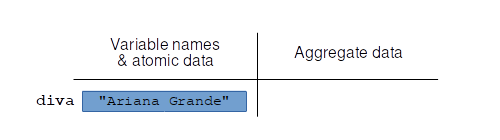
\includegraphics[width=0.9\textwidth]{bomb.png}
\end{center}

Now say we do this:

\begin{Verbatim}[fontsize=\small,samepage=true,frame=single,framesep=3mm]
new_var_name = diva.upper()
\end{Verbatim}

The result is this picture:

\vspace{-.2in}
\begin{center}
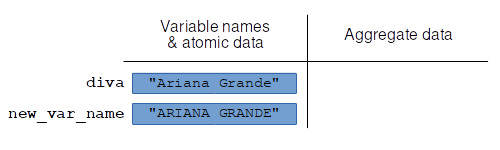
\includegraphics[width=0.9\textwidth]{bomb2.png}
\end{center}

And now we see the reason for it all. The contents of the \texttt{diva}
variable itself are \textit{\textbf{unchanged}} by the method call. Calling
``\texttt{.upper()}'' on \texttt{diva} didn't change the string value in
\texttt{diva}: it merely \textit{returned} a modified \textit{copy} of the
string.

Think of it this way: if I asked you, ``what is your name in Pig Latin?'' and
you told me, that would not intrinsically \textit{change} your actual name to
be in Pig Latin. You would simply be ``returning'' to me the Pig Latin version
of it in response to my query.

You could argue this behavior of Python's is dumb, or at best misleading, and
I'm actually inclined to agree with you in this case. But of course beggars
can't be choosers: someone took the time to write the \texttt{.upper()} method
for us, so if we want to take advantage of it we have to use his/her owner's
manual. And the fact is that many (perhaps even most) Python functions/methods
-- including many of the ones from Pandas, which we'll use extensively -- are
coded with this style: not actually modifying the variables they are passed,
but instead returning to you a modified copy which you must store.

Now given that this is the case, it would at least be nice if I could tell you
that it always, consistently worked this way. Then you could simply accept it
and get used to it. Alas, no. There \textit{are} functions/methods (lots of
them) which \textit{do} modify a parameter or the variable they were called on.
So sometimes, our na\"{i}ve approach of calling the method and expecting the
variable to change is exactly what we need to do. The bottom line is:
\textit{there's no way of knowing without being told, or else reading the
documentation.} We'll learn how to do the latter in a future chapter. For now,
I'm simply telling you for the record that the methods in
Figure~\ref{fig:stringOps} are all of the ``return a modified copy'' type, and
giving you a heads up that both styles of method do exist out there in
abundance.

A couple more things. First, as a corollary of the above, realize that the
following statement (on a line by itself) is officially 100\% useless:

\begin{Verbatim}[fontsize=\small,samepage=true,frame=single,framesep=3mm]
name_of_pet.lstrip()
\end{Verbatim}

You called the \texttt{.lstrip()} method, and then....did nothing with the
return value. If you don't store it in a variable -- or else do something with
it right away like \texttt{print} it before it slips out of your fingers --
it's irrevocably lost: it doesn't even show up on the memory picture because
there's no variable name. (Think about that.)

Second, note the following pattern which is very often used:

\begin{Verbatim}[fontsize=\small,samepage=true,frame=single,framesep=3mm]
name_of_pet = name_of_pet.lstrip()
\end{Verbatim}

Here, we're calling \texttt{.lstrip()} on the \texttt{name\_of\_pet} variable
\textit{and then storing the return value back in the \texttt{name\_of\_pet}
variable}. This might be what you thought would have happened in the first
place -- the author of the previous, useless line, probably wanted the variable
itself to permanently have its leading spaces removed. Simply calling
\texttt{.lstrip()} on the variable won't do that, but putting the revised value
back in the same blue box on the memory diagram will.


% note that "variable" means something different in this chapter. Not a single
% value, but multiple measurements.

\chapter{Scales of measure}

In the last chapter, we learned the Python verbiage for how to do arithmetic
operations. In this one, we zoom out and ask: when does it actually make
\textit{sense} to use those operations? The answer turns out to be: not always.

\index{syntax}
\index{semantics}
\index{meaning}
Another way to phrase this distinction is in terms of \textbf{syntax}
vs.~\textbf{semantics}. Syntax concerns the rules for combining various symbols
in a programming (or other) language. Semantics concerns the \textit{meaning}
of those symbols. This isn't something a programming language can tell us. Only
a human who understands what all those symbols refer to can determine when a
particular combination actually relates to something meaningful. Let this
chapter be your guide.

\index{scales of measure}
\section{The four scales of measure}

Every variable we collect can have various values, and the nature of
information it contains can be described by its \textbf{scale of measure}.
There are four of these\footnote{According to psychologist Stanley Smith
Stevens in 1946. Other researchers have developed related, but different,
scales of measure.}, and each one determines which kinds of operations are
``legal'' (\textit{i.e.}, sensible) with that variable.

\index{categorical variable}
\index{nominal variable}
\subsection{Categorical/nominal}

The first one is the simplest, although it actually has two different names in
common use: \textbf{categorical} or \textbf{nominal} variables. It is the scale
of variables that represent ``one of a set of choices,'' where no choice is
``higher'' or ``greater'' than any other.

\index{order}
An example would be a \texttt{fave\_color} variable that holds the value of a
child's favorite color: legal values are \texttt{"red"}, \texttt{"blue"},
\texttt{"green"} or \texttt{"yellow"}. We know it's categorical from, among
other things, the fact that there's no one right way to \textbf{order} those
values. (Alphabetical, most-popular-first, and ordering according to the
sequence of the rainbow are three possibilities. You might think of others.)

Political affiliation would be another categorical variable. Its values (like
\texttt{"Democrat"}, \texttt{"Republican"}, and \texttt{"Green"}) aren't in any
particular order. (Although you might think of the traditional left-to-right
political spectrum, that's only one dimension of political party, and perhaps
not even the most important one.) Other examples include film's genre, a
student's nationality, and a football player's position.

Now you might be tempted to think, ``hmm...all the categorical examples so far
are textual, not numeric. Perhaps this scales of measure thing is just another
way of stating the variable type?'' Alas, no. For one, we'll see text variables
in the next category as well. For another, even data that on its surface seems
numeric can actually be categorical in disguise.

Consider the uniform number of an athlete. I might be interested in asking,
``which uniform number had the greatest professional athletes who chose it?''
24 is a good candidate: Willie Mays, Ken Griffey Jr., and Kobe Bryant all wore
that jersey number. Or maybe \#7 is the winner, with Mickey Mantle, John Elway,
and Cristiano Ronaldo. Either way, though, all that matters in this analysis is
\textit{which} uniform number an athlete chose, not ``how high'' or ``how
great'' that number is compared to others. No one in their right mind would say
that Peyton Manning (\#18) was ``twice the player'' Mia Hamm was (\#9), because
uniform numbers aren't really ``numbers'' at all: they're more like labels.

\subsubsection{Legal operations for categorical/nominal variables}

\index{mode}
\index{central tendency}
\index{measure of central tendency}
When a variable is on a categorical scale, about the only things you can do are
compare for equality/inequality, count the occurrences of different values, and
compute something called the \textbf{mode} of the set.

The mode simply means the value that occurs \textit{the most often}. It's the
first of the ``\textbf{measures of central tendency}'' we'll see: such measures
are a way of capturing something about the ``typical'' value of a variable. For
categorical variables, the only typical-ness is ``which one occurs the most
often?'' If we ask a bunch of people for their \texttt{fave\_color}, and we get
the answers \texttt{"blue"}, \texttt{"red"}, \texttt{"blue"}, \texttt{"blue"},
and \texttt{"yellow"}, then the mode is \texttt{"blue"}. It's that simple.

To wrap things up, these things make sense to ask of a \textit{categorical}
variable:

\begin{compactitem}
\item[\leftthumbsup] ``Is his favorite color the same as her favorite color?''
\item[\leftthumbsup] ``How many people have \texttt{"red"} as their favorite
color?''
\item[\leftthumbsup] ``What's the most popular favorite color?''
\end{compactitem}

while these do \textit{not}:

\begin{compactitem}
\item[\leftthumbsdown] ``Is his favorite color greater than her favorite
color?'' (??)
\item[\leftthumbsdown] ``What's Caitlin's favorite color minus Hannah's?'' (??)
\item[\leftthumbsdown] ``What's the `average' favorite color in this data
set?'' (??)
\end{compactitem}


\index{ordinal variable}
\index{order}
\subsection{Ordinal}

One step up on the food chain is an \textbf{ordinal} variable, which means that
its different possible values \textit{do} have some meaningful order.

Consider \texttt{education\_level}, a variable that contains the highest degree
a survey respondent has earned. Its values can be any of the following:
\texttt{"HS"}, \texttt{"Associates"}, \texttt{"Bachelors"}, \texttt{"Masters"},
and \texttt{"PhD"}. In some ways, this is like \texttt{fave\_color}: the
variable must take on one of a set of specific, prescribed values. However,
it's pretty clear that a High School degree is closer to (more similar to) an
Associates degree than it is to a Ph.D. Each successive value represents more
education, and so unlike categorical variables, it \textit{does} make sense to
compare them along greater-than-or-less-than lines.

In addition to the mode, another measure of central tendency available for
ordinal variables is the \textbf{median}. I think of the median as the
``middlest'' value: if you line up all the occurrences in a row -- in order of
the values -- it's the one that lies in the exact middle. Suppose our survey
respondents give these answers: \texttt{"Bachelors"}, \texttt{"HS"},
\texttt{"HS"}, \texttt{"Masters"}, \texttt{"Masters"}, \texttt{"Bachelors"},
and \texttt{"HS"}. To compute the median, we line them all up in order:

\begin{center}
\texttt{"HS"  "HS"  "HS"  "Bachelors"  "Bachelors"  "Masters"  "Masters"}
\end{center}

nd find the middlest one, which is \texttt{"Bachelors"}. So \texttt{"HS"} is
the mode of this variable, and \texttt{"Bachelors"} is the median.

Other examples of ordinal variables include an NCAA basketball team's top-25
ranking, a taxpayer's tax bracket, and survey questions asking whether you
\texttt{"strongly disagree"}, \texttt{"disagree"}, are \texttt{"neutral"},
\texttt{"agree"}, or \texttt{"strongly agree"} with a certain statement.

Again, a list. For \textit{ordinal} variables, these are okay:

\begin{compactitem}
\item[\leftthumbsup] ``Is his education level the same as her education level?''
\item[\leftthumbsup] ``How many people answered \texttt{"strongly disagree"} to
this question?''
\item[\leftthumbsup] ``Is UMW basketball ranked higher or lower than Messiah?''
\item[\leftthumbsup] ``What's the median tax bracket for this group of
employees?''
\end{compactitem}

and these are \textit{not}:

\begin{compactitem}
\item[\leftthumbsdown] ``Which looks like the bigger mismatch on paper: Duke
v.~Kentucky, or Villanova v.~Gonzaga?'' (??)
\item[\leftthumbsdown] ``What's Caitlin's education level minus Hannah's?'' (??)
\item[\leftthumbsdown] ``What's the `average' tax bracket for this group of
employees?''
\end{compactitem}

It's worth commenting on that second list, because you might have thought some
of those items were completely reasonable. For example, suppose that in the
latest AP poll, Duke is currently ranked \#1, Kentucky \#3, Villanova \#4, and
Gonzaga \#23. You might think that clearly the Villanova/Gonzaga matchup is the
most lopsided, since there's nineteen places between them, whereas Duke and
Kentucky are separated by just two.

But not necessarily. We know Duke is considered \textit{stronger} than
Kentucky, but not \textit{how much stronger}. It is almost certainly not the
case that the teams are exactly evenly spaced all the way down the list from
\#1 to \#25. Real life doesn't work like that. Instead, it might be the case
that Duke and Georgetown, the \#1 and \#2 teams in the country, are considered
\textit{far and away} the best two teams. And perhaps the next five or even
twenty teams on the list are considered very close, to the point where experts
disagree wildly on what order they should be in. If this is the case, then
mighty Duke vs.~(comparatively) lowly Kentucky might be an enormous mismatch,
while Villanova and Gonzaga is considered a tossup.

\index{order}
\index{spacing}
The bottom line is: although an ordinal variable's values are \textit{ordered},
there is no information at all about the \textit{spacing} between them. I'll
tell you from personal experience that the difference between a Bachelors and a
Masters degree is nuthin' compared to that between a Masters and a Ph.D. (You
can ask anyone who has earned the latter for confirmation.)

This leads into the second item on the no-no list: subtracting two ordinal
values. All you're going to get is ``the number of positions in the sequence by
which they differ,'' which tells you next to nothing. If I ask people to rate a
movie on a scale of \texttt{"POOR"}, \texttt{"FAIR"}, \texttt{"GOOD"}, and
\texttt{"EXCELLENT"}, the difference between \texttt{"POOR"} and
\texttt{"GOOD"} is likely to be a lot greater than that between \texttt{"FAIR"}
and \texttt{"EXCELLENT"}. This is true even though the ``difference'' between
them seems exactly the same: ``two ranking's worth.'' The fact is that humans
don't interpret those four adjectives as exactly equally spaced, and therefore
it's a fallacy to interpret their results as though they did.

Which leads to the third and last item: trying to take the ``average'' (adding
up all the scores and dividing by the total). It's tempting to say, ``let's
treat \texttt{"POOR"} as a 1, \texttt{"FAIR"} as a 2, \texttt{"GOOD"} as a 3,
and \texttt{"EXCELLENT"} as a 4. Then, we can just take the mean of all the
results to get the average rating! What's not to like?'' What's not to like is
that by assigning those numbers, you added spurious information and thereby
twisted the respondent's meaning into something they didn't necessarily intend.
They very likely didn't think of the four options as equally-spaced
numerically, and so this average is quite bogus. Instead, take the median.



% TODO:
%    .append() with ignore_index=True
%     OR maybe just .reset_index(drop=True)   (more general purpose)
%
% memory diagrams, including .copy()

\chapter{Three kinds of aggregate data}
\label{ch:aggregateData}

Now it's time to consider some loftier goals for our lowly atomic bits of data.
Most anything interesting in Data Science comes from arranging them together in
various ways to form more complex structures. This chapter is the subject of
these.

\index{aggregate data}
\index{variable!aggregate}
\section{Aggregate data types}

The number of ways in which pieces of data can be arranged is far greater than
the number of different atomic types. These various ways all have names, some
of them nerdy and/or exotic like ``hash tables,'' ``binary search trees,'' and
``skip lists.'' Nevertheless, there are again three basic ones which will form
the basis of our study: they're called \textbf{arrays}, \textbf{associative
arrays}, and \textbf{tables}. As before, we'll consider each one conceptually
first, and then look at how to use them in Python.

\index{array}
\subsection{Arrays}

\index{element}
An \textbf{array} is simply a sequence of items, all in a row. We call those
items the ``\textbf{elements}'' of the array. So an array could have ten whole
numbers as its elements, or a thousand strings of text, or a million real
numbers.

\index{homogeneous}
\index{heterogeneous}
Normally, we will deal with \textbf{homogeneous} arrays, in which all the
elements are of the same type; this turns out to be what you want 99\% of the
time. Some languages (including Python) do permit creating a
\textbf{heterogeneous} array, which could hold (say) three whole numbers,
sixteen reals, and four strings of text all mixed together. But usually you're
using an array to contain a bunch of related values, like the current balances
of all the accounts in your bank, or the Twitter screen names of all a user's
followees.

Figure~\ref{fig:array} shows what those two examples would look like
conceptually. One has four strings of text, and the other five real numbers.
Note that each \textit{entire set} of elements is \textit{one} variable. We
might call the left one ``\texttt{followees}'' and the right one
``\texttt{balances}.''

\begin{figure}[ht]
\centering
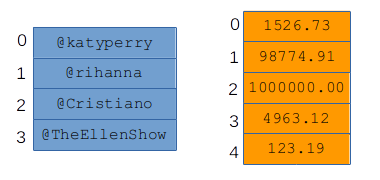
\includegraphics[width=0.6\textwidth]{array.png}
\caption{Two arrays.}
\label{fig:array}
\end{figure}

\index{index@index (pl:~indices)}
\label{arrayIndex}

Worthy of special note are the numbers on the left-hand side. These numbers
are called the \textbf{indices} (singular:~\textbf{index}) of the array.
They exist simply so we have a way to talk about the individual elements. I
could say ``element \#2 of the \texttt{followees} array'' to refer to
\texttt{@Cristiano}.

\index{zero@zero, starting at}
And yes, you noticed that the index numbers start with 0, not 1. Yes, this is
weird. The reason I did that it is because nearly all programming languages
(including Python) number their array elements starting with zero, so you might
as well just start getting used to it now. It's really not hard once you get
past the initial weirdness.

Arrays are the most basic kind of aggregate data there is, and they are the
workhorse of a whole lot of Data Science processing. Sometimes they're called
\textbf{lists}, \textbf{vectors}, or \textbf{sequences}, by the way. (When a
particular concept has lots of different names, you know it's important.)

\index{array!associative}
\index{key-value pair}
\subsection{Associative arrays}
\label{sec:assocArrays}

An \textbf{associative array}, by contrast, has no index numbers. And its
elements are slightly more complicated: instead of just bare values, an
associative array contains \textbf{key-value pairs}.
Figure~\ref{fig:assocArray} shows a couple of examples. The left-hand side of
each picture shows the keys, and the right-hand side the corresponding value.

With an associative array, you don't ask ``what's element \#3?'' like you do
with a regular array. Instead, you ask ``what value is associated with the
\texttt{"Washington"} key?'' And out pops your answer (\texttt{"Redskins"}).

\begin{figure}[ht]
\centering
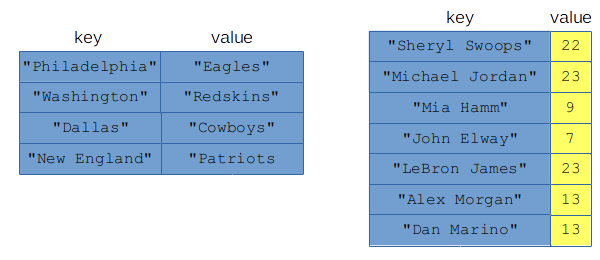
\includegraphics[width=0.9\textwidth]{assocArray.png}
\caption{Two associative arrays.}
\label{fig:assocArray}
\end{figure}

\index{order}
\index{undefined}
\index{mapping (a key to a value)}
All access to the associative array is through the keys: you can change the
value that goes with a key, retrieve the value that goes with a key, or even
retrieve and process \textit{all} the keys and their associated values
sequentially.\footnote{Using something called a ``loop,'' which we'll learn
about a little later in the book.} In that third case, the order in which
you'll receive the key-value pairs is \textbf{undefined} (which means ``not
guaranteed to be consistent'' or ``not necessarily what you'd expect.'') This
underscores the fact that there isn't any reliable ``first'' key-value pair,
or second, or last. They're just kind of all equally ``in there.'' Your mental
model of an associative array should just think of keys that are
\textbf{mapped} to values (we say that \texttt{"Dallas"} is ``mapped'' to
\texttt{"Cowboys"}) without any implied order. (Sure, the
\texttt{"Philadelphia"}/\texttt{"Eagles"} pair is at the top of the picture,
but that's only because I had to put \textit{something} at the top of the
picture, and I chose Philadelphia at random. It doesn't have any meaningful
primacy though.)

\index{homogeneous} Note a couple things about Figure~\ref{fig:assocArray}.
First, the keys in an associative array will almost always (and for us,
\textit{always}) be homogeneous. Similarly, the values will be homogeneous. But
the keys might not be of the same type as the values. In the left picture, both
keys and values are text, but in the right picture, the keys are text and the
values (uniform numbers of famous athletes) are whole numbers. This is
perfectly healthy and good.

\index{uniqueness!of keys in an associative array}
Second, realize that the \textit{keys} in an associative array must be
\textbf{unique} -- this means that there can be no duplicate keys. If we tried
to create a second \texttt{"Alex Morgan"} (oh, if only...) with a different
value, that new value would \textit{replace} Alex's current value, not sit
alongside the first one as an additional key-value pair.

The reverse is not true, however: the \textit{values} of an associative array
may very well not be unique. In the left-hand picture they are, but in the
right-hand picture there are duplicates: both Jordan and LeBron wore \#23 in
their stellar careers, while Hall of Famer quarterback Dan Marino once chose
the same uniform number that Alex wears today. This isn't a problem, because we
always access the information in an associative array \textit{through the
keys}. Asking ``what number did Mia Hamm wear?'' gives us a well-defined
answer. Asking ``which famous athlete wore \#23?'' does not. That's why we
can't ask that second question (and aren't meant to).

\subsection{Tables}

\index{table}

Lastly, we have the table, which in Data Science is positively ubiquitous. In
Figure~\ref{fig:table} we return to the pinterest.com example, with a table of
their most popular users. As you can see, it has more going on that than the
previous two aggregate data types. Still, it's pretty straightforward to wrap
your head around.

\begin{figure}[ht]
\centering
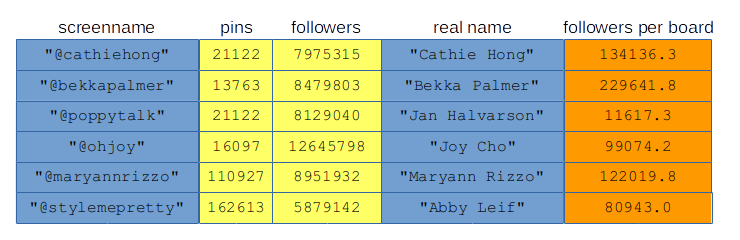
\includegraphics[width=\textwidth]{table.png}
\caption{A table.}
\label{fig:table}
\end{figure}

\index{row (of a table)}
\index{column (of a table)}
Unlike the other two aggregate data types, tables are full-on two-dimensional.
There's (theoretically) no limit to how many \textbf{rows} and how many
\textbf{columns} they can have. By the way, it's important to get those two
terms straight: rows go across, and columns go up and down. (Think of the
columns in the Trinkle Rotunda.) Also, the typical table has many, many more
rows than columns, so they're super tall and skinny, not short and fat.

\index{heterogeneous}
\index{homogeneous}
Although the \textit{rows} of a table are often heterogeneous, each
\textit{column} must be homogeneous. You can see that with a glance at
Figure~\ref{fig:table}. Each column represents a specific type of data -- in
this case, some statistic or piece of information about a Pinterest user.
Clearly all screen names should be of a text type, all ``number of pins or
followers'' should be whole numbers, \textit{etc.} It doesn't make sense
otherwise.

\index{order}
\label{assocArraysUnordered}
As with the other types, the whole dog-gone table -- no matter how many
millions of rows it might have -- is \textit{one} variable with a single name.
Also, just like with associative arrays, there normally isn't any implied
\textit{order} to the rows. Many implementations of these data types (including
Python/Pandas) will actually let you specify ``the first row'' or ``the
$53^{\textrm{rd}}$ row,'' but that always makes me cringe because conceptually,
there isn't any such thing. They're just ``rows'' that are all ``in
there.''

\subsubsection{``Querying'' tables (and other things)}

\index{query}
\label{tablesHaveNoKey}

Now you might be wondering how to actually ``get at'' the individual values of
a table. Unlike arrays, there's no index number. And unlike associative arrays,
there's no key. How then to address, say, the \texttt{@poppytalk} row?

The answer will turn out to be something called a \textbf{query}, which is a
geeky way of saying ``a set of criteria which will match some, but not all, of
the rows and/or columns.'' For instance, we might say ``tell me the pin count
for \texttt{@ohjoy}.'' Or, ``give me all the information for any user who has
more than 100,000 followers per board \textit{and} at least 20,000 pins.''
Those specific requirements will restrict the table to a subset of its rows
and/or columns. We'll learn the syntax for that later. It's a bit tricky but
very powerful.

\index{element}
By the way, it turns out we'll actually be using the concept of a query for
arrays and associative arrays as well. So strictly speaking, a query isn't just
a ``table thing.'' However, they're especially invaluable for tables, since
they're essentially the \textit{only} way to access individual elements.

\section{Aggregate data and memory pictures}

Recall from chapter~\ref{ch:memoryPictures} (p.~\pageref{fig:memoryPicture})
that the right-hand side of our memory pictures bore the label
``\textsf{Aggregate data}.'' You may have anticipated that that's where the
stuff in this chapter will live, and you're right. But there's a catch.
Remember that variable \textit{names} live on the left-hand side, and that's
true even if the variable is of an aggregate type! This turns out to be
crucially important, so I'm going to make a big deal about it.

You must draw your memory pictures (either on a whiteboard, or in your head) in
a very specific way, and that way is illustrated in
Figure~\ref{fig:aggregateMemory}.

\begin{figure}[ht]
\centering
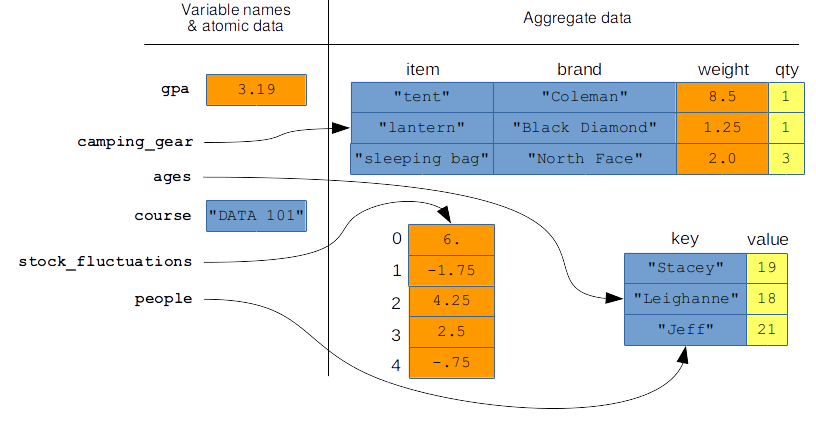
\includegraphics[width=1\textwidth]{aggregateMemory.png}
\caption{Where aggregate data variables -- and their variable names -- live in
memory.}
\label{fig:aggregateMemory}
\end{figure}

Study this picture carefully, and notice several vitally important things.
First, \textit{all} the variable names are on the left-hand side -- whether
aggregate or not. This is always, always true.

\index{pointer}
\index{reference}

Second, the actual array, associative array, and table depicted in this diagram
are on the right-hand side. The variable name on the left ``\textbf{points
to}'' the data in question with a little arrow. The technical name for this
arrow is a \textbf{pointer} or a \textbf{reference}. The rule is simple: each
atomic variable (like \texttt{gpa} or \texttt{course}) contains \textit{the
colored box itself}. Aggregate variables (like the other four) contain
\textit{a pointer to the group of colored boxes.}

Finally, mull over the fact that two \textit{different} variables in this
memory picture are pointing to the same thing! (\texttt{ages} and
\texttt{people}) Believe it or not, this is a normal occurrence. The
consequence is that if Stacey had a birthday, and we increased her age from 19
to 20 in the associative array, \textit{both} \texttt{ages} \textit{and}
\texttt{people} would automatically see the new value. There is only one copy
of that associative array in memory, and both variable names point at it.

It may seem like I'm being pedantic with this left-side-right-side stuff and
all the little arrows. \textbf{I promise you I'm not.} The moment your data
analysis program gets even mildly complicated, you will do the \textit{wrong}
thing and get the \textit{wrong} answers if you don't think of it exactly like
this. Take your time and commit it to memory.


% np.array([]), np.arange(), np.zeros(),
% np.loadtxt("file", dtype=object, delimiter='!!!')
% +, -, *, /
% np.sqrt()
% np.round( , num_decimals)
% np query syntax

% indexing, slices

\chapter{Arrays in Python: NumPy \texttt{ndarray}s}

\index{array!in NumPy}
\index{ndarray@\texttt{ndarray} (NumPy)}
\index{list@\texttt{list}, plain-ol'}
There are several candidates in the Python language for representing the type
of array structure we introduced in chapter~\ref{ch:aggregateData}. One is the
plain-ol' Python \textbf{\texttt{list}}, which you may have used if you've
taken a computer science course in Python. Turns out, \texttt{list}s are going
to be too slow for us once we start dealing with a lot of data, plus there are
a lot of things that it won't do for us automatically that are handy to have.
Another choice is the Pandas \texttt{Series} which we'll actually cover in
chapter~\ref{ch:pythonAssocArrays} -- oddly, that one turns out to do too
\textit{much}, rather than too little, for our purposes here. A happy medium is
the \textbf{\texttt{ndarray}} from the NumPy package\footnote{Most people seem
to pronounce this ``NUM-pie,'' although I've heard ``NUM-pee'' as well. Pick
your poison.}. Before we do that, however, we need to learn what a ``package''
actually is, and how to use one.

\section{Packages}
\index{package}

Back in my day (circa 1990's) when someone wanted to write a computer program,
they wrote the entire thing themselves, line by line. Everything you needed to
do -- from something complex like making a remote network connection to
something simple like computing the average of some numbers -- was up to you to
build. Code sharing over the Internet just wasn't much of a thing.

Today, the reverse is true. When you write a complex data analysis program,
\textit{most} of the code will actually be written by others, if you do it
right. This is because many, many smart people across the globe have written
snippets of code to do all the common (and some not-so-common) things you'll
want to do, and your job is to string them all together. Put another way:
you're given most of the Legos\textsuperscript{\textregistered} -- and even a
bunch of pre-assembled chunks made with dozens of
Legos\textsuperscript{\textregistered} each -- and your job is to construct
your masterpiece out of those building blocks.

\index{package}
\index{importing (a package)}
\index{package}
\index{calling a function@``calling'' a function}
\index{calling a method@``calling'' a method (on a variable)}
In Python, a \textbf{package} is a repository of useful functions and methods
that someone else has written. By \textbf{import}ing a package into your
program, you're making all those useful things available to you. Your own code
can then call those functions/methods whenever you see fit. It's the modular,
organized, and elegant way to do things, in addition to saving a ton of time.

The first package we'll use is called \textbf{NumPy}, which stands for
``Numerical Python.'' To import it, you should include this exact line of code
in the \textit{first} Code cell of your Notebook:

\begin{Verbatim}[fontsize=\small,samepage=true,frame=single,framesep=3mm]
import numpy as np
\end{Verbatim}

Note that it's in all lower-case letters. Once that cell has been executed, you
now have access to all the NumPy ``stuff,'' which is the subject of this
chapter.

\section{The NumPy \texttt{ndarray}}

\index{array}
\index{ndarray@\texttt{ndarray} (NumPy)}
\index{matrix}
The actual data type that the NumPy package provides is called an
\texttt{ndarray}, which stands for ``n-dimensional array.'' If that sounds
heady, it kind of is, although in this course we're only ever going to use a
\textit{one}-dimensional array, which is super simple to understand. In fact,
it looks exactly like the examples in Figure~\ref{fig:array}
(p.~\pageref{fig:array}). ``One-dimensional'' just means that there is a single
index number, and the elements are all in a line.\footnote{A two-dimensional
array is a spreadsheety-looking thing also called a \textbf{matrix}. Each
element has \textit{two} index numbers: a row and a column. A three-dimensional
array is a cube, with three index numbers needed to specify an element.
\textit{Etc.}}

\subsection{Creating \texttt{ndarray}s}

There are many different ways to create an \texttt{ndarray}. We'll learn four
of them.

\subsubsection{Way 1: \texttt{np.array([])}}

\index{array@\texttt{array()} function (NumPy)}
The first is to use the \texttt{array()} function of the NumPy package, and
give it all the values explicitly. Here's the code to reproduce the
Figure~\ref{fig:array} examples:

\begin{Verbatim}[fontsize=\scriptsize,samepage=true,frame=single,framesep=3mm]
followees = np.array(['@katyperry','@rihanna','@Cristiano','@TheEllenShow'])
balances = np.array([1526.73, 98774.91, 1000000, 4963.12, 123.19])
\end{Verbatim}

\index{boxies (square brackets)}
\index{[]@\texttt{[]} (boxies)}
\index{bananas (parentheses)}
\index{()@\texttt{()} (bananas)}
It's simple, but don't miss the syntactical gotcha: \textit{you must include a
pair of boxies inside the bananas.} Why? Reasons.\footnote{For the experienced
reader, what we're actually doing here is creating a plain-ol' Python list
(with the boxies), and then calling the \texttt{array()} function with that
list as an argument.} For now, just memorize that for this function -- and this
function only -- we use ``\texttt{([}\textsl{...stuff...}\texttt{])}'' instead
of ``\texttt{(}\textsl{...stuff...}\texttt{)}'' when we call it.

\index{package}
\index{function}
\index{method}
By the way, the attentive reader might object to me calling \texttt{array()} a
function, instead of a method. Isn't there a word-and-a-dot before it, and
isn't that a ``method thing?'' Shrewd of you to think that, but actually no,
and the reason is that ``\texttt{np}'' isn't the name of a variable, but the
name of a \textit{package}. When we say ``\texttt{np.array()}'' what we're
saying is: ``Python, please call the \texttt{array()} function \textit{from the
\texttt{np} package}.'' The word-and-dot syntax does double-duty.

\index{type@\texttt{type()}}
We can call the \texttt{type()} function, as we did back on
p.~\pageref{typeFunction}, to verify that yes indeed we have created
\texttt{ndarray}s:

\begin{Verbatim}[fontsize=\small,samepage=true,frame=single,framesep=3mm]
print(type(followees))
print(type(balances))
\end{Verbatim}

\begin{Verbatim}[fontsize=\small,samepage=true,frame=leftline,framesep=5mm,framerule=1mm]
numpy.ndarray
numpy.ndarray
\end{Verbatim}

\index{dtype@\texttt{.dtype} (NumPy)}
This is useful, but sometimes we want to know what underlying atomic data type
the array is comprised of. To do that, we attach ``\texttt{.dtype}''
(confusingly, \textit{without} bananas this time) to the end of the variable
name. ``\texttt{.dtype}'' stands for ``data type.'' Here goes:

\begin{Verbatim}[fontsize=\small,samepage=true,frame=single,framesep=3mm]
print(type(followees))
print(type(balances))
\end{Verbatim}

\begin{Verbatim}[fontsize=\small,samepage=true,frame=leftline,framesep=5mm,framerule=1mm]
dtype('<U13')
dtype('float64')
\end{Verbatim}

Whoa, what does \textit{that} stuff mean? It's a bit hard on the eyes, but let
me explain. The underlying data type of \texttt{followees} is (bizarrely)
``\texttt{<U13}'' which in English means ``strings of Unicode
characters\footnote{A ``Unicode character'' is just a fancy way of saying ``a
character, which might not be English.'' NumPy is capable of storing more than
just a-b-c's in its strings; it can store symbols from Greek, Arabic, Chinese,
\textit{etc.} as well.}, each of which is 13 characters long or less.'' (If you
bother to count, you'll discover that the longest string in our
\texttt{followees} array is the last one, \texttt{'@TheEllenShow'}, which is
exactly 13 characters long.) The ``\texttt{float64}'' thing means
``\texttt{float}s, each of which is represented with 64 bits\footnote{A ``bit''
-- which is short for ``binary digit'' -- is the tiniest piece of information a
computer can store: it's a single 0 or 1.} in memory.

You don't need to worry about any of those details. All you need to know is: if
an array's \texttt{dtype} has ``\texttt{<U}'' in it, then it's composed of
strings; and if it has the word ``\texttt{int}'' or ``\texttt{float}'' in it,
it means one of those two old friends from chapter~\ref{ch:atomicData}.

\index{homogeneous}
\index{list@\texttt{list}, plain-ol'}
Incidentally, you'll recall from chapter~\ref{ch:aggregateData} that an array
is \textit{homogeneous}, which means all its elements are of the same type.
NumPy enforces this. If you try to combine them:

\begin{Verbatim}[fontsize=\small,samepage=true,frame=single,framesep=3mm]
weird = np.array([3, 4.9, 8])
strange = np.array([18, 73.0, 'bob', 22.8])
\end{Verbatim}

\index{type@\texttt{type()}}
you'll discover that NumPy converts them to all be of the same type:

\begin{Verbatim}[fontsize=\small,samepage=true,frame=single]
print(weird)
print(weird.dtype)
print(strange)
print(strange.dtype)
\end{Verbatim}

\begin{Verbatim}[fontsize=\small,samepage=true,frame=leftline,framesep=5mm,framerule=1mm]
[ 3.   4.9  8. ]
dtype('<U3')
['18' '73.0' 'bob' '22.8']
dtype('float64')
\end{Verbatim}

See how the \texttt{int}s \texttt{3} and \texttt{8} from the first array were
converted into the \texttt{float}s \texttt{3.}~and \texttt{8.}; meanwhile, all
of the numerical elements of the second array got converted to \texttt{str}s.
(If you think about it, that's the only direction the conversions could go.)

\subsubsection{Way 2: \texttt{np.zeros()}}

\index{increment}
\index{decrement}
\index{counter variable}

It will often be useful to create an array, possibly a large one, with all
elements equal to \textit{zero} initially. Among other scenarios, we often need
to use a bunch of counter variables to, well, count things. Suppose, for
example, that we had a giant array that held the numbers of likes that each
Instagram photo had. When someone likes a photo, that photo's appropriate
element in the array should be \textbf{incremented} (raised in value) by one.
Similarly, if someone unlikes it, then its value in the array should be
\textbf{decremented} by one.

\index{zeros@\texttt{zeros()} function (NumPy)}
An easy way to do this is NumPy's \texttt{zeros()} function:

\begin{Verbatim}[fontsize=\small,samepage=true,frame=single,framesep=3mm]
photo_likes = np.zeros(40000000000)
\end{Verbatim}

(although I'll bet you don't have enough memory on your laptop to actually
store an array this size! Instagram sure has a lot of pics...) When I do this
on my Data Science cluster, I get this:

\begin{Verbatim}[fontsize=\small,samepage=true,frame=single,framesep=3mm]
print(photo_likes)
print(photo_likes.dtype)
\end{Verbatim}

\begin{Verbatim}[fontsize=\small,samepage=true,frame=leftline,framesep=5mm,framerule=1mm]
array([ 0.,  0.,  0., ...,  0.,  0.,  0.])
float64
\end{Verbatim}

Don't miss the ``\texttt{...}'' in the middle of that first line! It means
``there are (potentially) a lot of elements here that we're not showing, for
conciseness.'' Also notice that \texttt{zeroes()} makes an array of
\texttt{float}s, not \texttt{int}s.


\subsubsection{Way 3: \texttt{np.arange()}}

\index{arange@\texttt{arange()} function (NumPy)}
Sometimes we need to create an array with regularly-spaced values, like ``all
the numbers from one to a million'' or ``all even numbers between 20 and 50.''
We can use NumPy's \texttt{arange()} function for this.

\index{type@\texttt{type()}}
Normally we pass this function two arguments, like so:

\begin{Verbatim}[fontsize=\small,samepage=true,frame=single,framesep=3mm]
usa_years = np.arange(1776, 2020)
print(usa_years)
print(usa_years.dtype)
\end{Verbatim}

\begin{Verbatim}[fontsize=\small,samepage=true,frame=leftline,framesep=5mm,framerule=1mm]
[1776 1777 1778 1779 ... 2016 2017 2018 2019]
int64
\end{Verbatim}

If you read that code and output carefully, you should be surprised. We asked
for elements in the range of 1776 to 2020, and we got...1776 through
\textit{2019}. Huh?

\index{OBOE@OBOE (off-by-one error)}
\index{off-by-one error}

Welcome to one of several little Python idiosyncrasies. When you use
\texttt{arange()} you get an array of elements starting with the first
argument, and going up through \textit{but not including} the last number.
There's a reason Python and NumPy decided to do it this way\footnote{Certain
common operations are claimed to be ``simpler'' when you make a range function
work this way. I personally don't buy it: I think it should work in the way you
probably expected (including the second argument). I didn't get a vote,
though.}, but for now it's just another random thing to memorize. If you
forget, you're likely to get an ``OBOE'' -- which stands for ``off-by-one
error'' -- a common programming error where you do \textit{almost} the right
thing but perform one fewer, or one more, operation than you meant to.

Anyways, other than that glitch, you can see that the function did a useful
thing. We can quickly generate regularly-spaced arrays of any range of values
we like. By including a third argument, we can even specify the \textbf{step
size} (the interval between each pair of values):

\begin{Verbatim}[fontsize=\small,samepage=true,frame=single,framesep=3mm]
twentieth_century_decades = np.arange(1900, 2010, 10)
prez_elections = np.arange(1776, 2024, 4)
print(twentieth_century_decades)
print(prez_elections)
\end{Verbatim}

\begin{Verbatim}[fontsize=\small,samepage=true,frame=leftline,framesep=5mm,framerule=1mm]
[1900 1910 1920 1930 1940 1950 1960 1970 1980 1990 2000]
[1776 1780 1784 1788 ... 2008 2012 2016 2020]
\end{Verbatim}

Notice we had to specify 2010 and 2024 as the second argument to these function
calls in order for the arrays to include 2000, and 2020, respectively. This is
the same ``up to but not including the end point'' behavior, but extended to
step sizes of greater than one.



% memory pics


% TODO: np.sqrt()
% TODO: slices

\chapter{Arrays in Python (2 of 2)}
\label{ch:arraysInPython2}

\index{array!in NumPy}
\index{ndarray@\texttt{ndarray} (NumPy)}

Now that we know several options for how to \textit{create} \texttt{ndarrays},
what can we do with them? Many and sundry things.

\section{Getting the array size}

To learn how long an array is (\textit{i.e.}, how many elements) we use the
\texttt{len()} function, kind of like we did for strings. Refer back to
Figure~\ref{fig:arraysInMemory} (p.~\pageref{fig:arraysInMemory}) and consider
this code:

\begin{Verbatim}[fontsize=\footnotesize,samepage=true,frame=single,framesep=3mm]
num_players = len(roster)
sam_len = len(roster[2])
big_number = len(photo_likes)
print("There are {} players on the USWNT.".format(num_players))
print("Sam Mewis has {} characters in her name.".format(sam_len))
print(big_number)
print("We've had {} elections.".format(len(prez_elections)))
\end{Verbatim}

\begin{Verbatim}[fontsize=\footnotesize,samepage=true,frame=single,framesep=3mm]
There are 24 players on the USWNT.
Sam Mewis has 9 characters in her name.
40000000000
We've had 59 elections.
\end{Verbatim}

\label{overloading}
\index{overloading}
\index{return@``returning'' a value}
\index{array!length}
\index{len@\texttt{len()}}
\index{element}
This is an example of Python \textbf{overloading} function names, which just
means that the same name is used for two different functions. When you pass a
string to \texttt{len()}, you get the number of characters; but when you pass
an array to \texttt{len()}, you get the number of elements it has.
(The \texttt{roster} array had way more than 24 \textit{letters} in it, notice
-- but \texttt{len()} returned 24 since that was the number of strings.)

\section{Accessing individual elements}

\subsection{Retrieving an element}

\index{boxies (square brackets)}
\index{[]@\texttt{[]} (boxies)}
\index{element}
To get the value of a specific element from an array, we use ``boxie notation''
with the index number:

\begin{Verbatim}[fontsize=\small,samepage=true,frame=single,framesep=3mm]
print(prez_elections[0])
third_year = usa_years[2]
print("{} was the 3rd year of U.S.A.".format(third_year))
print("The highest-numbered player is {}".format(
    roster[len(roster)-1]))
\end{Verbatim}

\begin{Verbatim}[fontsize=\small,samepage=true,frame=leftline,framesep=5mm,framerule=1mm]
1788.0
1778 was the 3rd year of U.S.A.
The highest-numbered player is Christen Press.
\end{Verbatim}

Remember, indices start at zero (not one) so that's why the first line has a
\texttt{0} in it.

Now examine that last line, which is kind of tricky. Whenever you have boxies,
you have to first evaluate the code \textit{inside} them to get a number. That
number is then the index number Python will look up in the array. In the last
line above, the code \textit{inside} the boxies is:

\quad\quad\quad   ...\texttt{len(roster)-1}...

Breaking it down, we know that \texttt{len(roster)} is 24, which means
\texttt{len(roster)-1} must be 23, and so \texttt{roster[len(roster)-1]} is
\texttt{Christen Press}. It's a common pattern to get the last element of an
array.\footnote{Fun fact: you can also use \textit{negative} indices to mean
``from the end of the array, rather than the beginning.'' So
\texttt{roster[-1]} will also give you \texttt{Christen Press},
\texttt{roster[-2]} is \texttt{Jessica McDonald},
\texttt{roster[-5]} is \texttt{Crystal Dunn}, \textit{etc.} (see
p.~\pageref{rosterNames} for the values). I find this a bit obscure, though, so
I don't normally use this feature. (Negative indices also mean a completely
different thing in the R language, which is another reason I eschew them in
both R and Python.)}

To test your understanding, figure out what the following code will print:

\label{indexTest}
\begin{Verbatim}[fontsize=\small,samepage=true,frame=single,framesep=3mm]
q = 2
r = np.array([45,17,39,99])
s = 1
print(r[q-s+1]+3)
\end{Verbatim}

The answer is at the end of the chapter.

\subsection{Changing an element}

To modify an element of an array, just use the equals sign like we do for
variables:

\index{stooges@Stooges (The Three)}
\index{beavis@Beavis}
\begin{Verbatim}[fontsize=\small,samepage=true,frame=single,framesep=3mm]
stooges = np.array(['Larry','Beavis','Moe'])
print(stooges)
stooges[1] = 'Curly'
print(stooges)
\end{Verbatim}

\begin{Verbatim}[fontsize=\small,samepage=true,frame=leftline,framesep=5mm,framerule=1mm]
['Larry' 'Beavis' 'Moe']
['Larry' 'Curly' 'Moe']
\end{Verbatim}

After all, an individual element like \texttt{stooges[1]} is itself a variable
pretty much like any other.

% Omit: slices

\section{``Vectorized'' arithmetic operators}

Recall our table of Python math operators (Figure~\ref{fig:mathOps} on
p.~\pageref{fig:mathOps}). What do those things do if we use them on aggregate,
instead of atomic data? The answer is: something super cool and useful.

\subsection{Operating on an array and a single value}

Consider the following code:

\label{vectorizedArrayIntExample}
\begin{Verbatim}[fontsize=\small,samepage=true,frame=single,framesep=3mm]
num_likes_today = np.array([6,61,0,0,14])
num_likes_tomorrow = num_likes_today + 3
print(num_likes_tomorrow)
\end{Verbatim}

\begin{Verbatim}[fontsize=\small,samepage=true,frame=leftline,framesep=5mm,framerule=1mm]
[ 9 64 3 3 17 ]
\end{Verbatim}

See what happened? ``Adding 3'' to the \textit{array} means adding 3 \textit{to
each element}. All in one compact line of code, we can do five -- or even five
billion -- operations. This works for all the other Figure~\ref{fig:mathOps}
operators as well.

\index{vectorized@``vectorized'' operation}

For somewhat geeky reasons, this sort of thing is called a \textbf{vectorized}
operation. All you need to know is that this means \textbf{fast}. And that's
``fast'' in two different ways: fast to write the code (since instead of using
a \textbf{loop}, which we'll cover in \ref{ch:loops}, you just write a single
statement with \texttt{+} and \texttt{=} signs), and more importantly, fast to
\textit{execute}. For more geeky reasons, the above code will run lightning
fast even if \texttt{num\_likes\_today} had five hundred million elements
instead of just five. As you'll learn if you ever try it, a Python loop is much
slower.\footnote{I just ran that comparison on my laptop, and here are the
results. Using the plain-ol' ``\texttt{+}'' vectorized operator, my machine
added the number 3 to an array with five hundred million elements in just 1.51
seconds. A loop, by contrast, took 2.8 \textit{minutes} to do the same thing.}

Don't get me wrong: there are times we'll have to use a loop because we have no
choice. But the general rule with Python is: if you can figure out how to
perform a calculation without using a loop, always do it!


\subsection{Operating on two arrays}

\index{vectorized@``vectorized'' operation}

Possibly even cooler, we can even ``\texttt{+}'' (or ``\texttt{-}'', or
``\texttt{*}'', or...) two entire \textit{arrays} together. Example:

\label{vectorizedArrayArrayExample}
\begin{Verbatim}[fontsize=\small,samepage=true,frame=single,framesep=3mm]
salaries = np.array([38000, 102000, 55750, 29500, 250000])
raises = np.array([1000, 4000, 2000, 1000, 2000])
salaries = salaries + raises
print(salaries)
\end{Verbatim}

This code produces:

\begin{Verbatim}[fontsize=\small,samepage=true,frame=leftline,framesep=5mm,framerule=1mm]
[ 39000 106000 57750 30500 252000]
\end{Verbatim}

Can you see why? ``Adding'' the two arrays together performed addition
\textit{element-by-element}. The result is a new array with $38000+1000$ as the
first element, $102000+4000$ as the second, \textit{etc.} This, too, is a
lightning-fast, vectorized operation, and it too works with all the other math
operators.

Just to re-emphasize one point before we go on. In the example back on
p.~\pageref{vectorizedArrayIntExample}, we assigned the result of the operation
to a new variable, \texttt{num\_likes\_tomorrow}. This means that
\texttt{num\_likes\_today} itself was \textit{unchanged} by the code. In
contrast, in the example we just did, we assigned the result of the operation
back into an \textit{existing} variable (\texttt{salaries}). So
\texttt{salaries} has itself been updated as a result of that code.

% TODO: could include memory picture to this effect.


\section{Copying -- and \textit{not} copying -- arrays}

\label{copyingNotCopyingArrays}
\index{copying@copying (arrays)}
Now, a surprise for the unwary. Suppose I write this code:

\label{code:refNotCopy}
\begin{Verbatim}[fontsize=\small,samepage=true,frame=single,framesep=3mm]
stooges = np.array(['Larry','Beavis','Moe'])
funny_people = stooges
stooges[1] = 'Curly'
print("The stooges are: {}.".format(stooges))
print("The funny people are: {}.".format(funny_people))
\end{Verbatim}

Take a moment and predict what you think the output will be. Then, read it and
(possibly) weep:

\begin{Verbatim}[fontsize=\small,samepage=true,frame=leftline,framesep=5mm,framerule=1mm]
The stooges are: ['Larry' 'Curly' 'Moe'].
The funny people are: ['Larry' 'Curly' 'Moe'].
\end{Verbatim}

Note carefully: \textit{no \texttt{Beavis}}.

\begin{figure}[ht]
\centering
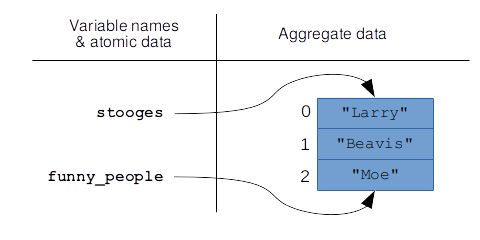
\includegraphics[width=0.49\textwidth]{refNotCopy.png}
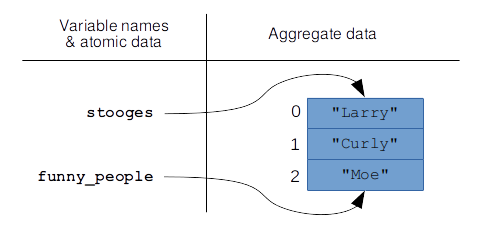
\includegraphics[width=0.49\textwidth]{refNotCopy2.png}
\caption{The code on p.~\pageref{code:refNotCopy} immediately before (left
side) and after (right side) the line ``\texttt{stooges[1] = \textquotesingle
Curly\textquotesingle}'' is reached.}
\label{fig:refNotCopy}
\end{figure}

\index{memory!picture}

Now the question is why. To understand this (and virtually any other tricky
programming problem) you have to return once again to the memory picture.
Figure~\ref{fig:refNotCopy} shows the situation immediately before, and after,
the line ``\texttt{stooges[1] = \textquotesingle Curly\textquotesingle}''
executes. Crucially, \textit{there is only one array} in memory. Both variables
-- \texttt{stooges} and \texttt{funny\_people} -- are pointing at it.

You see, if \texttt{y} contains \textit{aggregate} (instead of atomic) data,
the line ``\texttt{x = y}'' does not perform a copy operation. Instead, it just
points the \texttt{x} variable name to the same place \texttt{y} is pointing
to.

Once you grasp this, it's easy to see why \texttt{"Beavis"} completely
disappeared. There's only one array at all, so changing \texttt{stooges} has
the side effect of implicitly changing \texttt{funny\_people} as well.

\subsection{Actually copying}

The ``point the variable to the same thing, but don't do a copy'' behavior is
the default, because such copy operations are expensive (in terms of memory
usage and time to execute). They're normally not what you want anyway.
Sometimes, however, you \textit{do} want to produce an entire separate copy of
an array, so you can modify the copy yet preserve the original. To do so, you
use the \texttt{.copy()} method:

\begin{Verbatim}[fontsize=\footnotesize,samepage=true,frame=single,framesep=3mm]
orig_beatles = np.array(['John', 'Paul', 'George', 'Pete'])
beatles = orig_beatles.copy()
beatles[3] = 'Ringo'
print("The Beatles were originally {}.".format(orig_beatles))
print("But the ones we all know were {}.".format(beatles))
\end{Verbatim}

Look carefully at that second line: it makes all the difference. Instead of
making the new variable \texttt{beatles} point to the same array in memory that
\texttt{orig\_beatles} did, we explicitly copied the array and made
\texttt{beatles} point to that new copy. The final memory picture is thus as
per Figure~\ref{fig:copyNotRef}, and the output is of course:

\begin{Verbatim}[fontsize=\footnotesize,samepage=true,frame=leftline,framesep=5mm,framerule=1mm]
The Beatles were originally ['John' 'Paul' 'George' 'Pete'].
But the ones we all know were ['John' 'Paul' 'George' 'Ringo'].
\end{Verbatim}

\begin{figure}[ht]
\centering
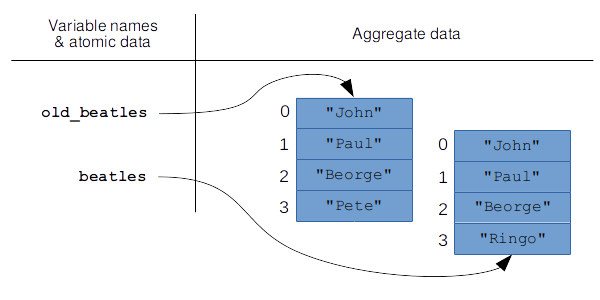
\includegraphics[width=0.9\textwidth]{copyNotRef.png}
\caption{The memory picture after calling the \texttt{.copy()} method, instead
of simply assigning to a new variable.}
\label{fig:copyNotRef}
\end{figure}


\section{Sorting arrays}

\label{sortingArrays}
\index{sorting@sorting (arrays)}
\index{int@\texttt{int}}
\index{float@\texttt{float}}
\index{str@\texttt{str}}
A common operation in Data Science is to \textbf{sort} an array, either
numerically (if the array contains \texttt{int}s or \texttt{float}s) or
alphabetically (if it contains strings). There are two ways to do this, which
turn out to differ in exactly the same was as the operations in the previous
section.

\index{on@``on''}
\index{sort@\texttt{.sort()}}
\index{in place@``in place''}
\index{calling a method@``calling'' a method (on a variable)}
One way is to call the \texttt{.sort()} method directly \textbf{on} an array.
This sorts the array \textbf{in place}, which means that the actual data in
memory is rearranged right then and there. As an important side effect, any
\textit{other} variable that points to the same array will \textit{also} be
sorted.

Here's an example:

\begin{Verbatim}[fontsize=\small,samepage=true,frame=single,framesep=3mm]
gpas = np.array([2.86, 3.99, 3.12, 1.17])
gpas2 = gpas.copy()
gpas3 = gpas
gpas.sort()
print("gpas has: {}".format(gpas))
print("gpas2 has: {}".format(gpas2))
print("gpas3 has: {}".format(gpas3))
\end{Verbatim}

\begin{Verbatim}[fontsize=\small,samepage=true,frame=leftline,framesep=5mm,framerule=1mm]
gpas has: [1.17 2.86 3.12 3.99]
gpas2 has: [2.86 3.99 3.12 1.17]
gpas3 has: [1.17 2.86 3.12 3.99]
\end{Verbatim}

Do you see why that output was produced? It's because the memory picture after
the ``\texttt{gpas.sort()}'' line looks like Figure~\ref{fig:dotSortArray}. The
\texttt{gpas} variable really \textit{is} the \texttt{gpas3} variable, so when
one is sorted, the other automatically is. They're both distinct from
\texttt{gpas2}, though.

\begin{figure}[ht]
\centering
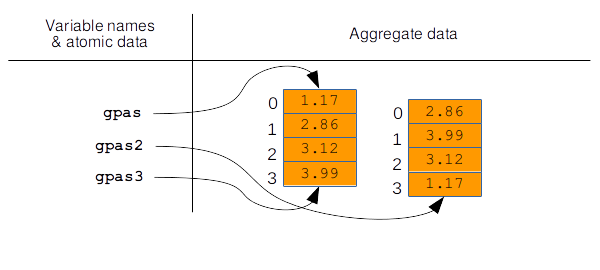
\includegraphics[width=0.9\textwidth]{dotSortArray.png}
\caption{The state of affairs after \texttt{.sort()}ing the \texttt{gpas} array in place.}
\label{fig:dotSortArray}
\end{figure}

\index{sorting@sorting (arrays)}
\index{sort@\texttt{np.sort()} (NumPy)}
\index{calling a function@``calling'' a function}
\index{passing an argument@``passing'' an argument}
The second option is to call the \texttt{np.sort()} function and pass an array
as an object. Like many Python functions, including the ones in the next
section, \texttt{np.sort()} \textit{returns a modified copy} of its argument
rather than changing it in place. To illustrate:

\index{Ravens, Baltimore}
\index{Patriots, New England}
\index{Broncos, Denver}
\index{Steelers, Pittsburgh}
\begin{Verbatim}[fontsize=\small,samepage=true,frame=single,framesep=3mm]
nfl_teams = np.array(["Ravens", "Patriots", "Broncos",
    "Chargers", "Steelers"])
sorted_teams = np.sort(nfl_teams)
print(nfl_teams)
print(sorted_teams)
\end{Verbatim}

\begin{Verbatim}[fontsize=\small,samepage=true,frame=leftline,framesep=5mm,framerule=1mm]
['Ravens' 'Patriots' 'Broncos' 'Chargers' 'Steelers']
['Broncos' 'Chargers' 'Patriots' 'Ravens' 'Steelers']
\end{Verbatim}

\index{return value}
Observe that the \texttt{nfl\_teams} variable, even though we passed it to
\texttt{np.sort()}, was not \textit{itself} sorted. The \texttt{sorted\_teams}
variable, on the other hand, \textit{is} alphabetically sorted, because we
assigned the return value from \texttt{np.sort()} to it. Again, the memory
picture is shown in Figure~\ref{fig:npSortArray}.

\index{on@``on''}
\begin{figure}[ht]
\centering
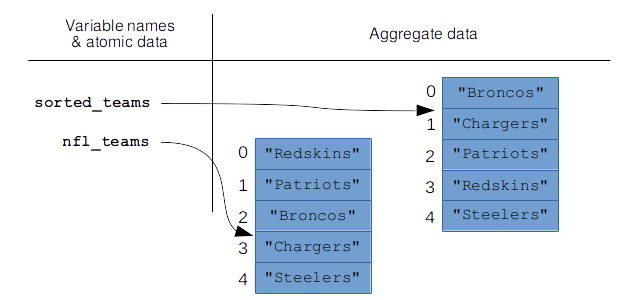
\includegraphics[width=0.9\textwidth]{npSortArray.pdf}
\medskip
\caption{Calling the \texttt{np.sort()} function (as opposed to calling the
\texttt{.sort()} method \textbf{on} the array) returns a sorted copy.}
\label{fig:npSortArray}
\end{figure}

To be clear, either one of these techniques can be used on \textit{any}
\texttt{ndarray}: whole numbers, real numbers, or text. I just chose to do real
numbers in the first example and text in the second. The difference between the
two is merely in what is affected: in one, the actual array in memory is
modified, and in the other, a modified copy is returned.

\section{More exotic array modifications}

\index{in place@``in place''}
There are lots of additional things you can do to an array to either modify its
structure or rearrange its contents. Here's a few. \textbf{Important: all of
the functions in this section return a modified copy of the array you pass to
it. They do \textit{not} change the array in place.}

\begin{itemize}
\itemsep.1em
\index{concatenating!arrays}
\index{append@\texttt{append()} (NumPy)}
\index{insert@\texttt{insert()} (NumPy)}
\index{delete@\texttt{delete()} (NumPy)}
\index{flip@\texttt{flip()} (NumPy)}
\index{reversing (an array)}
\item \texttt{np.append()} can be used to add a single element to the end of an
array, or to add an entire second array of elements to it. (In the latter case,
this is really \textbf{concatenation} of arrays.)
\item \texttt{np.insert()} is like the first form of \texttt{np.append()},
except it inserts in the middle (or the beginning).
\item \texttt{np.delete()} will remove an element of an array \textit{by
position}. In other words, you tell it which \textit{index number} to remove,
not which element.
\item \texttt{np.flip()} reverses the order of elements in an array.
\end{itemize}

These functions are all summarized in Figure~\ref{fig:handyNumPy}.

Remember that when you're calling a function like this -- which returns a
modified copy -- it is perfectly acceptable to store the return value
\textit{in the same variable} that you passed it. This is common if you don't
actually want to keep around the original:

\begin{Verbatim}[fontsize=\small,samepage=true,frame=single,framesep=3mm]
ice_cream_flavors = np.flip(ice_cream_flavors)
\end{Verbatim}

In this pattern, the net effect \textit{is} effectively to modify the array in
place, since you're making a reversed copy, and then assigning that reversed
copy to the same variable.

Anyway, here's some example code to illustrate the functions in this section:

\begin{Verbatim}[fontsize=\small,samepage=true,frame=single,framesep=3mm]
clowns = np.array(["Bozo", "Krusty"])
more_clowns = np.array(["Pennywise", "Skelton"])
more_clowns = np.insert(more_clowns, 1, "Happy Slappy")
all_clowns = np.append(clowns, more_clowns)
all_clowns = np.append(all_clowns, "Ronald McDonald")
all_clowns = np.flip(all_clowns)
all_clowns = np.delete(all_clowns, 2)
print("clowns is: {}".format(clowns))
print("more_clowns is: {}".format(more_clowns))
print("all_clowns is: {}".format(all_clowns))
\end{Verbatim}

\begin{Verbatim}[fontsize=\footnotesize,samepage=true,frame=leftline,framesep=5mm,framerule=1mm]
clowns is: ['Bozo' 'Krusty']
more_clowns is: ['Pennywise' 'Happy Slappy' 'Skelton']
all_clowns is: ['Ronald' 'Skelton' 'Pennywise' 'Krusty' 'Bozo']
\end{Verbatim}

% TODO: memory picture of the clowns

An \textit{excellent} exercise to help cement your understanding of the ideas
in this chapter would be to go through the above ``clowns'' code line by line,
drawing the memory picture as you go, and then confirm that your output matches
the actual output.

\smallskip

Yes, an \textit{excellent} exercise indeed!

\bigskip

\section[Characters within a string]{Postlude: characters within a string}

\index{string}
\index{str@\texttt{str}}

These two chapters have dealt with arrays, but let me say a word at this point
about \textit{strings}, and how they can be made to act like arrays in some
respects.

I mentioned earlier in the book (p.~\pageref{tiptoe}) that strings, though
normally treated as atomic, sometimes tiptoe up to the ``atomic/aggregate''
line and even cross it. In other words, we will occasionally look at individual
parts of a string variable rather than the entire thing as one lump.

\index{boxies (square brackets)}
\index{[]@\texttt{[]} (boxies)}

The way we access individual characters within a string is actually the same
boxie notation we use for arrays. So this code:

\vspace{-.15in}
\begin{Verbatim}[fontsize=\small,samepage=true,frame=single,framesep=3mm]
antihero = "Light Yagami"
print(antihero[0])
letter1 = antihero[6]
letter2 = antihero[7]
print("{}{}{}".format(letter1,letter2,letter1))
\end{Verbatim}
\vspace{-.1in}

will give this output:

\vspace{-.15in}
\begin{Verbatim}[fontsize=\small,samepage=true,frame=leftline,framesep=5mm,framerule=1mm]
L
YaY
\end{Verbatim}
\vspace{-.1in}

\index{zero@zero, starting at}

As you can see, string indexes use the same starting-at-zero nonsense that
arrays do. Hey, at least it's consistent.

\bigskip

\index{overloading}
This is actually another example of overloading. Just as the \texttt{len()}
function means two different things, depending on whether you're asking for the
length of an array or the length of a string (recall p.~\pageref{overloading}),
so the boxie notation means two different things. You're either getting a
specific element out of an array, or a specific character out of a string.

\section{Summary}

The table in Figure~\ref{fig:handyNumPy} gives the promised summary of
the array functions, methods, and operators in this chapter.

\setlength\extrarowheight{5pt}

\begin{figure}[ht]
\centering
\footnotesize
\begin{tabular}{c|p{3.1in}}
Function & Description \\
\hline

\texttt{len(}\textsl{arr}\texttt{)} & Get the number of elements in the array \textsl{arr}. \\

\textsl{arr}\texttt{[17]} & Get a specific element's value from the array \textsl{arr}. \\

\textsl{arr}\texttt{[8] =} (\textsl{something}) & Set a specific element of the array \textsl{arr}. \\

\textsl{arr} \texttt{+ 91} & Add a value to each element of \textsl{arr},
yielding a new array. (Also works with \texttt{-}, \texttt{*}, \texttt{/},
\textit{etc.}) \\

\textsl{arr1} \texttt{+} \textsl{arr2} & Add each pair of values in two arrays,
yielding a new array. (Also works with \texttt{-}, \texttt{*}, \texttt{/},
\textit{etc.}) \\

\textsl{arr1} = \textsl{arr2} & Make \textsl{arr1} point to the same data that
\textsl{arr2} points to. (\textit{Not} a copy!)\\

\textsl{arr1} = \textsl{arr2}\texttt{.copy()} & Make \textsl{arr1} point to a
new, independent copy of \textsl{arr2}. \\

\textsl{arr}\texttt{.sort()} & Sort the array \textsl{arr} \textbf{in place}. (Numerical or
alphabetical, depending on the \texttt{.dtype}.) \\

\texttt{np.sort(}\textsl{arr}) & Return a new array with the sorted elements
of \textsl{arr}. (Numerical or alphabetical, depending on the \texttt{.dtype}.)
\\

\texttt{np.append(}\textsl{arr}, \textsl{elem}\texttt{)} &
    Return a new array with \textsl{elem} tacked on to the end. \\

\texttt{np.append(}\textsl{arr1}, \textsl{arr2}\texttt{)} &
    Return a new array with the two arrays \textsl{arr1} and \textsl{arr2} concatenated. \\

\texttt{np.insert(}\textsl{arr}, \textsl{ind}, \textsl{val}\texttt{)} &
    Return a new array with the new value \textsl{val} inserted into position \textsl{ind} of \textsl{arr}. \\

\texttt{np.delete(}\textsl{arr}, \textsl{ind}\texttt{)} &
    Return a new array with the element at index \textsl{ind} removed from \textsl{arr}. \\

\texttt{np.flip(}\textsl{arr}\texttt{)} &
    Return a new array with \textsl{arr} in reverse order. \\
\end{tabular}
\bigskip
\caption{Handy NumPy functions, methods, and operators.}
\label{fig:handyNumPy}
\end{figure}

\vfill
\subsubsection{The answer}

\index{42 (Life, Universe, Everything)}
Oh, and the answer to the puzzle on p.~\pageref{indexTest} -- and also the
answer to Life, the Universe, and Everything, as it turns out -- is 42.



\chapter{Interpreting Data}

Let's take an intermission from the nitty-gritty Python stuff and talk about
how to properly \textit{interpret} the data we're working with; specifically,
how to draw correct conclusions from what we've collected.

\section{Independent and dependent variables}

\index{variable!dependent}
\index{variable!independent}
\index{independent variable (i.v.)}
\index{dependent variable (d.v.)}
\index{cause}
\index{causal}
\index{hiccup}
\index{greenhouse gas}
\index{smoking}
\index{lung cancer}
\index{global warming}

You've undoubtedly seen countless studies that claim to reveal important truths
about the world, such as that smoking can cause lung cancer, greenhouse gas
emissions can cause higher global temperatures, or orgasms can cure hiccups.
Much of the time, scientists try to find a \textbf{causal} factor that links
one variable to another: they suspect that the value of a variable $A$ (often
called the \textbf{independent variable}, or ``\textbf{i.v.}''~for short) is a
\textit{reason}, or \textbf{cause}, of a certain value in another variable $B$
(the \textbf{dependent variable}, or ``\textbf{d.v.}'').

Just to avoid misunderstandings, when we claim that $A$ \textbf{causes} $B$, we
don't normally mean that it \textit{exclusively} causes it, or even that it
\textit{reliably} causes it. There are lots of contributing factors to lung
cancer besides smoking, after all; and tons of smokers never develop cancer. We
simply mean that $A$ is a contributing factor to $B$, and that the value of the
$A$ variable exerts some, but not total, influence over the value of the $B$
variable.

\index{variable}
\index{objects (of a study)}

Importantly, we're using the word \textbf{variable} here in a different, but
related way than we used it in chapters~\ref{ch:atomicData},
\ref{ch:arraysInPython1}, and \ref{ch:arraysInPython2}. As we did in
chapter~\ref{ch:scalesOfMeasure} (see p.~\pageref{variableDifferent} footnote),
we use ``variable'' here to mean a specific aspect of the \textbf{objects of a
study} that can differ, or ``vary.'' The objects in our study (often people,
but sometimes companies, organizations, environments, nations, \textit{etc.})
\textit{each} have a value for the variable. Thus if you think of a
``per-capita income'' variable, you might think of an entire \textit{array} of
floats, each of which represented the average income-per-resident of a single
nation.

\index{scales of measure}
\index{categorical variable}

The variables in question can be from any of the scales of measure from
chapter~\ref{ch:scalesOfMeasure}. Take the smoking example, with patients as
the object of study. We might say that independent variable $A$ is categorical,
with values \texttt{SMOKER} and \texttt{NON-SMOKER}. The dependent variable $B$
is also categorical: \texttt{CANCER} and \texttt{NO-CANCER}. The key question
is: do people with $A=\texttt{SMOKER}$ also have $B=\texttt{CANCER}$
\textit{more often} (a higher percentage of the time) than people with
$A=\texttt{NON-SMOKER}$ do?

\index{ratio variable}
\index{interval variable}

In the greenhouse gas emissions example, our objects of study might be
\textit{years}. Our variables are both numeric, with $A$ (a measure of yearly
greenhouse gas emissions, measured in gigatonnes $\textrm{CO}_2$) on the ratio
scale, and $B$ (average worldwide temperature increase/decrease) on an interval
scale. Here, the question would be: do years in which $A$ is relatively high
typically also have $B$ relatively high? Put another way: do years in which
earthlings have released more gas into the atmosphere tend to correspond with
years in which the global temperature increased?

And of course, we might have one categorical variable and one numeric. Perhaps
our objects of study are American adults, and while our categorical $A$
variable has values \texttt{DEMOCRAT}, \texttt{REPUBLICAN}, \texttt{OTHER}, and
\texttt{INDEPENDENT}, our numerical $B$ is yearly income. Our question would
be: do adherents of one political party tend to be more wealthy than those of
another?

Or, flipping sides, the independent variable $A$ could be numeric while the
dependent variable $B$ is categorical. Our objects of study might be high
school seniors applying to UMW. Let $A$ be the number of different colleges a
student applied to, and $B$ a categorical variable with values
\texttt{ADMITTED-TO-UMW} and \texttt{NOT-ADMITTED-TO-UMW}. The question of
interest is here is: do students who apply to more colleges tend to get in to
UMW more often?

\section{Association and causality}

\label{association}

All of the above questions can be answered with data. In future chapters, we'll
learn the exact Python commands to ask them, and how to interpret the answers.

\index{association}
\index{correlation}
\index{dependent}

For now, I merely want to draw your attention to the fact that these are all
questions of \textbf{association}, not causation. An association between
variables merely means that they are \textbf{correlated} in some way
statistically.\footnote{Another way to put this is to say that the variables
are \textbf{dependent} on each other, although this is confusing because we're
already using the word ``dependent'' to refer to one of the variables.} If
$A=\texttt{SMOKER}$ goes with $B=\texttt{CANCER}$ more often than
$A=\texttt{NON-SMOKER}$ does, then there \textit{is} an association between the
two, period. If yearly income $B$ is on average higher for
$A=\texttt{REPUBLICAN}$ than for $A=\texttt{DEMOCRAT}$, then there \textit{is}
an association between the two, period.

\label{howMuchMore}

(By the way, a key nuance will turn out to be: \textit{how much} more often
does $A=\texttt{SMOKER}$ need to go with $B=\texttt{CANCER}$ in order for us to
be confident that there is a true association? Or \textit{how much} more
wealthy do the $A=\texttt{REPUBLICAN}$s need to be on average for us to have
confidence we've identified a real link to political party? That one's a little
tricky, and we'll postpone addressing it for now.)

\index{causality}
\label{pythonAssociation}

So anyway, the question of association turns out to be pretty straightforward
to answer. Python will simply tell us if variables are associated or not. More
difficult, however, is determining \textbf{causality}
(a.k.a.~\textbf{causation}). Does a person's political affiliation influence
how much wealth they have? Or is it the other way around: does a person's
wealth cause them to vote a certain way? Or is it neither of these, with some
third factor (perhaps values, or life philosophy) helping determine
\textit{both} variables?

\index{$\rightarrow$@$\rightarrow$ (causality)}

If the first of these three is the case, we would write ``$A \rightarrow B$,''
pronounced ``$A$ causes $B$''. If the second, we'd write, ``$B \rightarrow
A$,'' and for the third, we'd write ``$C \rightarrow A, B$'' for some other
(possibly yet to be determined) variable $C$. Determining which (if any) of
these is true calls for some careful thinking, intuition, and additional kinds
of statistical tests.

In fact, just to blow your mind, Figure~\ref{fig:causalityTypes} gives a
partial list of the various types of causation that \textit{could} be the true
explanation, once we find out that $A$ and $B$ have an association. As you can
see, there are a lot of ways to go wrong. Only \textit{one} of the
possibilities is that ``$A$ actually causes $B$,'' which is what we suspected
in the first place. The others are all ways of producing that same association
we picked up in the data.

\begin{figure}[ht]
\small
\centering
\begin{tabular}{|c|c|p{3.3in}|}
\hline
Symbology & Name & Example \\
\hline
\multirow[c]{2}{*}{$A \rightarrow B$} & \multirow[c]{2}{*}{causation} & Regular
exercise does indeed normally lead to a lower resting heart rate. \\
\hline
\multirow[c]{2}{*}{$B \rightarrow A$} & \multirow[c]{2}{*}{reverse causation} & Smoking doesn't cause depression;
depression causes smoking. \\
\hline
\multirow[c]{2}{*}{$C \rightarrow A, B$} & \multirow[c]{2}{*}{\makecell{external causation \\ (confounding
factor)}} & Ice cream sales don't cause shark attacks; high temperatures boost both ice
cream sales and ocean swimming. \\
\hline
\multirow[c]{2}{*}{$A \rightarrow B$ \& $B \rightarrow C$} &
\multirow[c]{2}{*}{multiple causation }& A liberal arts
education does improve critical thinking skills, but lots of other things do
too. \\
\hline
\multirow[c]{2.5}{*}{$A,C \rightarrow B$} & \multirow[c]{2.5}{*}{joint causation} &
Just being tall doesn't necessarily make you a good basketball player, but if
your height is accompanied by another factor as well (athleticism), then you
will be. \\
\hline
\multirow[c]{2.5}{*}{$A \rightarrow C \rightarrow B$} &
\multirow[c]{2.5}{*}{indirect causation} & People who use antiperspirant tend to
get more dates, but it's not because of the antiperspirant \textit{per se};
it's because they don't have an unpleasant odor. \\
\hline
\multirow[c]{3}{*}{$A \not\rightarrow B$} & \multirow[c]{3}{*}{spurious
association} & Although for many years the outcome of the Washington Redskins
game immediately preceding a Presidential election predicted the election's
outcome, that was by coincidence. \\
\hline
\end{tabular}
\medskip
\caption{Various types of causality that could be the underlying reason why an
association between $A$ and $B$ exists.}
\label{fig:causalityTypes}
\normalsize
\end{figure}

\section{Confounding factors}

\index{confounding factor}
\index{external causation}
\index{variable!confounding}

Let me speak to two of the items in the Figure~\ref{fig:causalityTypes} table
in particular. The third one on the list, \textbf{external causation}, is a
case where a third variable (call it $C$) comes into play. We refer to this as
a \textbf{confounding factor} (or \textbf{confounding variable}) because it
``confounds'' us: causes us to interpret the meaning behind the data in an
incorrect way. The example in the table is a famous and funny one: clearly
sharks don't react to Ben \& Jerry's daily net profits, and people (probably)
don't run out and buy ice cream to cope with their anxiety about shark attacks.
Neither $A \rightarrow B$ nor $B \rightarrow A$, but a third variable -- hot
days -- influence both of them.

\index{causal diagram}
\index{barbecue}
\index{cancer}
\label{barbecue}

Now of course it's not always this obvious. Here's an example I ran across
recently. A magazine article reported on a new health scare: scientists have
discovered that \textit{eating barbecue can increase your risk of cancer.}
Pictorially, this claim is illustrated in the \textbf{causal diagram} in
Figure~\ref{fig:causalDiagram}, which shows our i.v.~and our d.v.~; the arrow
means exactly what it meant earlier.

\begin{figure}[ht]
\centering
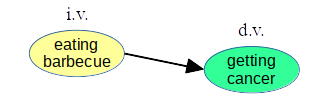
\includegraphics[width=0.6\textwidth]{causalDiagram.png}
\caption{A hypothesis as to causality: eating barbecued foods increases one's
risk for certain types of cancer.}
\label{fig:causalDiagram}
\end{figure}

Unlike sharks and ice cream, this one seems plausible. And I'm not claiming to
have read enough about their study to tell whether the researchers' claim is
bogus. But I couldn't help thinking that there are a great many possibly
confounding factors that could be blurring the results. For one, choosing to
eat barbecue a lot is probably often associated with a less healthy, higher-fat
diet in general (I can speak from experience on that). If that's true, and if
high-fat diets -- whether featuring lots of barbecue or not -- are associated
with these same poor health outcomes, then we'd have the picture on the
left-side of Figure~\ref{fig:causalDiagram23}. The red bubble represents the
confounding factor, which is influencing both i.v.~and d.v. If this picture
were the correct one of the underlying phenomenon, then the correlation we
thought were picking up between barbecue and cancer was actually due to fat
content.

\begin{figure}[ht]
\centering
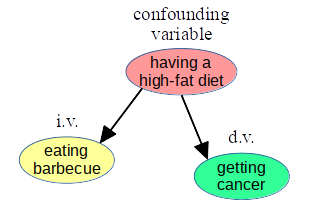
\includegraphics[width=0.4\textwidth]{causalDiagram2.png}
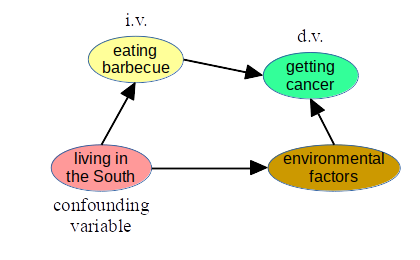
\includegraphics[width=0.5\textwidth]{causalDiagram3.png}
\caption{Other hypotheses as to causality, each resulting in the same
associations in the data, yet involving confounding factors.}
\label{fig:causalDiagram23}
\end{figure}

Another example is the right-hand side of Figure~\ref{fig:causalDiagram23}.
Perhaps barbecue is more popular culturally in some areas of the country (say,
the South, where I certainly see it eaten a lot), and perhaps those areas have
other environmental factors that can lead to cancer. In this case, the
``South'' confounder indirectly affects the d.v.~(via another variable,
representing the environment) but it still affects it.

It's not hard to think of others. These were just the first two that came to
mind. The point is that it's really hard to be sure you've thought of all of
them!


\subsection{Paranoia and overparanoia}

All this should lead you to be somewhat paranoid, but not
\textit{over}paranoid. Confounding variables can definitely lead us to make
mistakes in our reasoning, but perhaps they're not \textit{quite} as common as
you think. Understand that a confounding factor is \textit{not} simply any
other factor that affects the dependent variable. Instead, for a variable to be
confounding \textbf{it must affect both the independent \textit{and} the
dependent variable.}

Let me illustrate with an example. I suspect that on average, men are taller
than women. And I further suspect that there's causality here, and that it goes
from $A$ (sex) to $B$ (height), not the other way around. (Clearly people don't
spontaneously ``turn male'' because they reach a certain height.) So my
thinking on the subject is summed up in Figure~\ref{fig:sexHeight}.

\begin{figure}[ht]
\centering
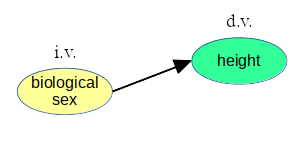
\includegraphics[width=0.6\textwidth]{sexHeight.png}
\caption{Stephen's hypothesis: a person's biological sex (male or female) plays
a causal role in determining their height.}
\label{fig:sexHeight}
\end{figure}

Now let me show you what I mean by ``overparanoia.'' What if someone said,
``but wait, Stephen, not so fast! You've got potential confounding variables
out the wazoo! Why, surely heredity plays some role in a person's height --
tall parents are more likely to have tall offspring, just due to genetics. And
nutrition, too, is a factor: it's been demonstrated that impoverished
communities suffering from malnutrition will have children with stunted growth.
And heck, if you're born at a high elevation (like Nepal), there's less
gravitational pull dragging your body down to earth, so it stands to reason
that you'll probably grow taller. And on and on!'' Figure~\ref{fig:sexHeight2}
depicts this (supposed) scientific nightmare.

\begin{figure}[ht]
\centering
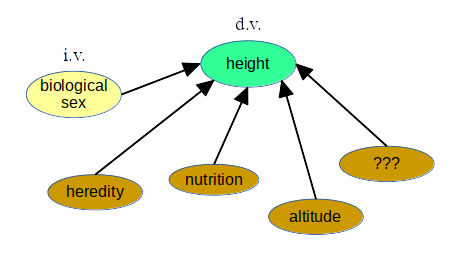
\includegraphics[width=0.7\textwidth]{sexHeight2.png}
\caption{Oh geez -- confounding variables galore? \textbf{\textit{No!}}}
\label{fig:sexHeight2}
\end{figure}

But plausible as some of those theories are, they are \textit{not} confounding
variables! These are simply \textit{other factors that may affect the d.v.}
Sure, they may also play a causal role in determining a person's height, but
they do \textit{not} invalidate our finding about sex and height.

For them to truly be confounders, they would have to affect the yellow
\textit{and} the green variable, and I'm pretty sure they do not. Do tall
parents tend to bear more sons, and short parents more daughters? If not, this
isn't a confounder. Do boys have more nutritious diets than girls? (In some
parts of the world, that may unfortunately be true, but I don't believe it is
in our country.) So that one isn't a confounder either. Having additional
causes of an effect does not nullify a genuine effect. Only a lurking variable
that pulls the marionette strings of both i.v.~and d.v.~can do that.

\section{Dealing with confounding factors}

\index{confounding factor}
\index{variable!confounding}

\label{smart}
Confounding factors are evil, and we must deal with them seriously. There are
essentially two ways to do that: one that requires us to be smart, and one that
requires us to have money.

\subsection{Controlling for a confounding factor}

\index{control (for a variable)}
\index{stratification}

If we anticipate that a certain variable may be a confounding factor, we can
\textbf{control} for it. There are several techniques for this, some of which
you'll learn in your statistics class, but the simplest one to understand
involves \textbf{stratification}.

\index{pinterest}

Let's make a silly example this time. We'll go back to the earlier pinterest
theme. I think I've noticed over the past few years that the heavy pinterest
users I know seem to almost always have long hair. I've developed a hypothesis
about this, which involves theories about how protein filaments in follicles
with longer protrusions lead to certain chemical changes in the brain. These
mind alterations, if unchecked, lead to increased creativity, craftiness, and a
desire to share artistic creations with other like-minded individuals. Further,
these aesthetic desires manifest themselves in increased usage of the
\texttt{pinterest.com} website, as measured in number of logins per day.

My theory is thus reflected in the causal diagram in
Figure~\ref{fig:hairPinterest}. Study it carefully.

\begin{figure}[ht]
\centering
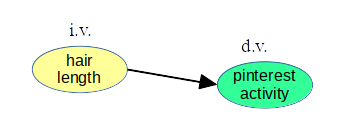
\includegraphics[width=0.6\textwidth]{hairPinterest.png}
\caption{A theory about how hair length impacts the number of times a person
logs on to pinterest each day.}
\label{fig:hairPinterest}
\end{figure}

Now of course this follicle stuff is bogus. I'm using an extreme example to
make a point. Quick, can you come up with a possible confounding factor? Yeah,
drr: \textit{gender}. It's undoubtedly true that women tend to (but don't
always) have longer hair than men, and it's undoubtedly true that
\texttt{pinterest.com} is a website that tends to appeal to (but not
exclusively to) women. And causality-wise, the arrows obviously flow from
gender, not to it: the pinterest login screen doesn't change your gender, and a
man won't turn into a woman simply by growing his hair long (although a
transgender woman might grow her hair long as a signal of her underlying gender
change.) 

Put that all together, and you get the much more plausible causal diagram in
Figure~\ref{fig:hairPinterest2}.

\begin{figure}[ht]
\centering
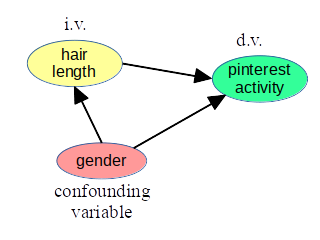
\includegraphics[width=0.6\textwidth]{hairPinterest2.png}
\caption{An alternative theory that holds that a person's gender influences
both their long-haired-ness and their pinterest-ness.}
\label{fig:hairPinterest2}
\end{figure}


\index{control (for a variable)}
\index{stratification}

Now then. Controlling for a confounding variable through stratification is done
by considering the objects of the study in \textit{groups}, comparing
\textit{only those who have the same (or similar) value for the confounding
variable.}

In this case, we would separate the men from the women in our study. Looking at
\textit{just the men}, we would ask, ``is longer hair associated with frequency
of pinterest logins?'' Then we would do the same, looking at \textit{just the
women.} Only if Python reported that both of these separate groups illustrated
such a trend would we (tentatively) conclude, ``hair length itself does play a
role in causing pinterest activity, \textit{even when controlling for
gender.}''

Do the thought experiment to see if you agree. I know the whole follicle theory
struck you as dumb (and hopefully, a little funny) to begin with. ``Of
\textit{course},'' you said to yourself, ``it's gender, not hair length, that's
drawing users to pinterest, dummy!'' But suppose we \textit{did} perform that
stratification technique, and discovered that the association actually
\textit{did} hold in both cases. Would that give it more credence in your mind?
It ought to. By stratifying, we've eliminated gender from the picture entirely,
and now we're faced with the facts that those with longer hair -- regardless of
gender -- log on to pinterest more often. 

\index{association}

Now I wrote the word ``tentatively'' a couple paragraphs ago, because there are
still some caveats. For one, we don't actually know that the causality goes in
the stated direction. Removing the gender confounder, we confirmed that there
is still an association between hair length and pinterest, but that association
might translate into a $B \rightarrow A$ phenomenon. Perhaps users who log on
to pinterest a lot see a lot of long-haired users, and (consciously or not)
decide to grow their own hair out as a result? That actually sounds more
plausible than the original silly theory. Either way, we can't confirm the
direction just by stratifying.

The other caveat is even more important, because it's more pervasive: just
because we got rid of one confounding variable doesn't mean there aren't
others. The whole ``control for a variable'' approach requires us \textit{to
anticipate in advance} what the possible confounding factors would be. This is
why I said back on p.~\pageref{smart} that this approach requires the
experimenter to be smart.

\subsection{Running a controlled experiment}

\index{controlled experiment}
\index{observational study}

The other way to deal with confounding variables is to run a \textbf{controlled
experiment} instead of an \textbf{observational study}. I jokingly said on
p.~\pageref{smart} that this option requires the experimenter to have money.
Let me explain.

% TODO: uhh...actually include the DGP chapter, as promised below.

\index{data-generating process (DGP)}
An observational study is one in which data is produced by naturally occurring
processes (we'll call them \textbf{data-generating processes}, or
\textbf{DGPs}, in a later chapter) and then collected by the researcher.
Crucially, the experimenter plays no role in influencing what any of the
variable values are, whether that be the i.v.~, the d.v.~, other related
variables, or even possible confounders. Everything just is what it is, and the
researcher is simply observing.

Now at first this sounds like the best of all possible worlds. Scientists are
supposed to be objective, and to do everything they can to avoid biasing the
results, right? True, but the sad fact is that \textit{every observational
study has potential confounding factors} and there's simply no foolproof way to
account for them all. If you \textit{knew} them all, you could potentially
account for them. But in general we don't know. It all hinges on our
cleverness, which is a bit like rolling the dice.

\index{randomization!of experimental subjects}
\index{controlled experiment}

A controlled experiment, on the other hand, is one in which \textit{the
researcher decides what the value of the i.v.~will be for each object of
study.} She normally does this randomly, which is why this technique is called
\textbf{randomization}.

Now controlled experiments bear some good news and some bad news. First, the
good news, which is incredibly good, actually: \textit{a controlled experiment
automatically eliminates \underline{every} possible confounding factor, whether
you thought of it or not.} Wow: magic! We get this boon because of how the
i.v.~works. The researcher's coin flip is the \textit{sole} determinant of who
gets which i.v.~value. That means that no other factor can be ``upstream'' of
the coin flip and influence it in any way. And this in turn nullifies all
possible confounding factors, since as you recall, a confounder must affect
both the i.v.~and the d.v.

The catch is that controlled experiments can be very expensive to run, and in
many cases can't be run at \textit{all}. Consider the barbecue example from
p.~\pageref{barbecue}. To carry out a controlled experiment, we would have to:

\begin{compactenum}
\item Recruit participants to our study, and get their informed consent.
\item Pay them some \$\$ for their trouble.
\item For each participant, flip a coin. If it comes up heads, \textit{that
person must eat barbecue three times per week for the next ten years.} If it's
tails, \textit{that person must never eat barbecue for the next ten years.}
\item At the end of the ten years, measure how many barbecuers and
non-barbecuers have cancer.
\end{compactenum}

There's a question of this even being ethical: if we suspect that eating
barbecue can cause cancer, is it okay to ``force'' participants to eat it? Even
past that point, however, there's the expense. Ask yourself: if you were a
potential participant in this experiment, how much money would you demand in
step 2 to change your lifestyle to this degree? You might love barbecue, or you
might hate it, but either way, it's a coin flip that makes your decision for
you. That's a costly and intrusive change to make.

Other scenarios are even worse, because they're downright impossible. We can't
flip coins and make (at random) half of our experimental subjects male
and the other half female. We can't (or at least, shouldn't) randomly decide
our participants' political affiliations, making one random half be Democrats
and the others Republicans. And we certainly can't dictate to the nations of
the world to emit large quantities of greenhouse gases in some years and small
quantities in others, depending on our coin flip for that year.

Bottom line: if you can afford to gather data from a controlled experiment
rather than an observational study, always choose to do so. Unfortunately, it
won't always be possible, and we'll have to rest on the uneasy assumption that
we successfully predicted in advance all the important confounding variables
and controlled for them.

\section{Spurious associations}

\index{spurious association}
\index{association!spurious}

Okay, back to Figure~\ref{fig:causalityTypes} on
p.~\pageref{fig:causalityTypes}. The other item I'd like to point out in that
table is the last one, which is called a \textbf{spurious association}. This is
written as ``$A \not\rightarrow B$,'' with the arrow crossed out. And it simply
means ``nope, none of the above: these variables actually aren't associated at
all.''

You might be scratching your head at that one. Didn't I tell you
(p.~\pageref{pythonAssociation}) that Python is smart enough to tell us
definitively whether or not two variables are associated? That was supposed to
be the easy part; the hard part was only in figuring out what \textit{causes}
that association. But now I'm saying that associations might not be
associations, and Python is powerless to know the difference!

\index{IQ}
The root cause of this state of affairs is obvious once you see it, and it has
to do with the ``how much more?'' questions from p.~\pageref{howMuchMore}.
Clearly, when we collect data, there's a ``luck of the draw'' component
ever-present. I might have data that suggests Republican voters have higher
income than Democratic voters...but it's of course possible that I just
happened to poll some richer Republicans and some poorer Democrats. Suppose I
told you I thought women were on average smarter than men, and in my random
sample the average men's IQ was 102.7 and the average woman's was 103.5. The
women's was indeed greater...but is that \textit{enough} greater? Is the
difference explainable simply by the randomness of my poll?

\index{bar}
The true answer is that we can \textit{never} know for absolute certainty,
unless we can poll the entire population. (Only if we measured the IQ of every
man and every woman on planet Earth, and took the means of both groups, could
we say which one truly had the higher mean.) But what we have to do is
essentially ``set a bar'' somewhere, and then determine whether we got over it.
We could say ``only if the average IQ difference is greater than 5 points will
we conclude that there's really a difference.''

\subsection{Setting $\alpha$}

\label{alpha}

Now the procedure for determining how high to put the ``bar'' is more
complicated and more principled than that. We don't just pick a number that
seems good to us. Instead, Python will put the bar at exactly the right height,
given the level of certainty we decide to require. Some things that influence
the placement of the bar include the sample size and how variable the data is.
The thing \textit{we} specify in the bar equation, however, is \textit{how
often we're willing to draw a false conclusion.}

\index{$\alpha$ (alpha)}
\index{alpha@alpha ($\alpha$)}

That quantity is called ``$\boldsymbol{\alpha}$'' (pronounced
``\textbf{alpha}'') and is a small number between 0 and 1. Normally we'll set
$\alpha=.05$, which means: ``Python, please tell me whether the average male
and female IQs were \textit{different enough} for me to be confident that the
difference was truly a male-vs-female thing, not just an idiosyncrasy of the
people I chose for my poll. And by the way, \textit{I'm willing to be wrong 5\%
of the time about that.}''

It seems weird at first -- why would we accept drawing a faulty conclusion 5\%
of the time? Why not 0\%? But you see, we have to put the bar somewhere. If we
said, ``I never want to think there's an association when there's not one,''
Python would respond, ``well fine, if you're so worried about it then I'll
never tell you there is one.'' There has to be some kind of criterion for
judging whether a difference is ``enough,'' and $\alpha=.05$, which is ``being
suckered only 1 in 20 times'' is the most common value for social sciences.
($\alpha=.01$ is commonly used in the physical sciences.)

So, the last entry in the Figure~\ref{fig:causalityTypes} table means ``even
though the $A$ and $B$ variables aren't \textit{really} associated at all -- if
we gathered some more $A$s and some more $B$s, we'd probably detect \textit{no}
association -- you were fooled into thinking there was one because our random
sample was a bit weird.'' There's really no way around this other than being
aware it can happen, and possibly repeating our study with a different data
set to be sure of our conclusions.


% Somewhere: .map() for recoding

\chapter[Associative arrays in Python (1 of 3)]{\huge\selectfont{Associative
arrays in Python (1 of 3)}}
\label{ch:assocArraysInPython1}

\index{associative array}
\index{Pandas package}
\index{package}
\index{importing (a package)}

Our next trick is to represent associative arrays (review
section~\ref{sec:assocArrays} if you need to) in Python. To do so, we will
use another package, which goes by the adorable name ``Pandas'':

\begin{Verbatim}[fontsize=\small,samepage=true,frame=single,framesep=3mm]
import pandas as pd
\end{Verbatim}

This code should go at the top of your first notebook cell, right under your
``\texttt{import numpy as np}'' line. The two go hand in hand.

\index{table}
\index{NumPy package}
\index{series@\texttt{Series} (Pandas)}
\index{dict@\texttt{dict} (dictionary)}

By the way, just as there were other choices besides NumPy \texttt{ndarray}s to
represent ordinary arrays, there are other choices in Python for associative
arrays. The native Python \texttt{dict} (``dictionary'') is an obvious
candidate. Because this won't work well when the data gets huge, however, and
because using Pandas now will set up our usage of tables nicely in the next
few chapters, we're going to use the Pandas \textbf{Series} data type for our
associative arrays.


\section{The Pandas \texttt{Series}}
\label{sec:creatingSeries}

\index{array!associative}
\index{key-value pair}
\index{series@\texttt{Series} (Pandas)}

A \texttt{Series} is conceptually a set of key-value pairs. The keys are
normally homogeneous, and so are the values, although the keys might be of a
different type than the values. Any of the three atomic types are permissible
for either.

\index{index@index (pl:~indices)}
\index{deep}

Somewhat confusing is that the Pandas package calls the keys ``the
\textbf{index},'' which is an overlap with the term we used for ordinary arrays
(see p.~\ref{arrayIndex}). It's not a total loss, though, since if you think
hard about it, you'll realize that in some sense, \textit{a regular array is
really just an associative array with consecutive integer keys.} Oooo, deep. If
you consider the two halves of Figure~\ref{fig:assocArraysAreArrays}, I think
you'll agree.

\begin{figure}[ht]
\centering
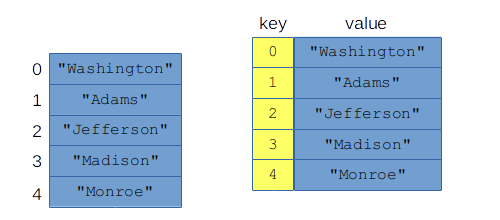
\includegraphics[width=0.9\textwidth]{assocArraysAreArrays.png}
\caption{An ordinary array, and an associative array, that represent the same
information.}
\label{fig:assocArraysAreArrays}
\end{figure}


\subsection{Creating \texttt{Series}es}

Here are a few common ways of creating a Pandas \texttt{Series} object in
memory.

\subsubsection{Way 1: create an empty \texttt{Series}}

Perhaps this first one sounds dumb, but we will indeed have occasion to start
off with an empty \texttt{Series} and then add key/value pairs to it from
there. The code is simple:

\begin{Verbatim}[fontsize=\small,samepage=true,frame=single,framesep=3mm]
my_new_series = pd.Series()
\end{Verbatim}

Voil\`{a}.

\subsubsection{Way 2: \texttt{pd.Series([], index=[])}}

As with NumPy \texttt{ndarrays}, we can explicitly list the values we want in a
new \texttt{Series}. We also have to list the \textbf{index} values (the keys).
The syntax for doing so is:

\label{marvelSeries}
\index{Marvel comics}

\begin{Verbatim}[fontsize=\small,samepage=true,frame=single,framesep=3mm]
alter_egos = pd.Series(['Hulk','Spidey','Iron Man','Thor'],
    index=['Bruce','Peter','Tony','Thor'])
\end{Verbatim}

This creates the \texttt{Series} shown in Figure~\ref{fig:Series}.

\begin{figure}[ht]
\centering
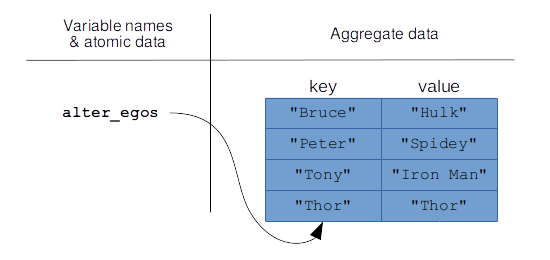
\includegraphics[width=0.8\textwidth]{Series.png}
\caption{A Pandas \texttt{Series} in memory.}
\label{fig:Series}
\end{figure}

\index{boxies (square brackets)}
\index{[]@\texttt{[]} (boxies)}
\index{bananas (parentheses)}
\index{()@\texttt{()} (bananas)}

Be careful to keep all your boxies and bananas straight. Note that both the
keys \textit{and} the values are in their own sets of boxies.

We can print (small) \texttt{Series}es to the screen to inspect their contents:

\begin{Verbatim}[fontsize=\small,samepage=true,frame=single,framesep=3mm]
print(alter_egos)
\end{Verbatim}

\begin{Verbatim}[fontsize=\small,samepage=true,frame=leftline,framesep=5mm,framerule=1mm]
Bruce        Hulk
Peter      Spidey
Tony     Iron Man
Thor         Thor
dtype: object
\end{Verbatim}

\index{type@\texttt{type()}}
\index{dtype@\texttt{.dtype} (NumPy/Pandas)}
and as we did on p.~\pageref{arrayType}, we can inquire as to both the
overarching type of \texttt{alter\_egos} and also to the kind of underlying
data it contains:

\begin{Verbatim}[fontsize=\small,samepage=true,frame=single,framesep=3mm]
print(type(alter_egos))
print(alter_egos.dtype)
\end{Verbatim}

\begin{Verbatim}[fontsize=\small,samepage=true,frame=leftline,framesep=5mm,framerule=1mm]
pandas.core.series.Series
object
\end{Verbatim}

Just as it did on p.~\pageref{dtypeRules}, the ``\texttt{object}'' here is just
a confusing way of saying ``\texttt{str}''. Don't read anything more into it
than that.

\subsubsection{Way 3: ``wrapping'' an array}

\label{wrap}
\index{dimension}

Associative arrays, and the Pandas \texttt{Series}es we've been using to
implement them, are inherently \textit{one}-dimensional data structures. This
is just like the NumPy arrays we used before. Pandas Serieses also provide a
bunch of features for manipulating, querying, computing, and even graphing
aspects of their content. It's a lot of rich stuff on top of plain-old NumPy.

\index{wrapping}

For this reason, it's common to want to create a \texttt{Series} that just
``wraps'' (or encloses) an underlying NumPy \texttt{ndarray}, and provides all
that rich stuff.

The way to do this is simple:

\begin{Verbatim}[fontsize=\small,samepage=true,frame=single,framesep=3mm]
my_numpy_array = np.array(['Ghost','Pumpkin','Vampire','Witch'])
my_pandas_enhanced_thang = pd.Series(my_numpy_array)
\end{Verbatim}

You can then treat \texttt{my\_pandas\_enhanced\_thang} as an ordinary
aggregate variable which has the more sophisticated operations of next chapter
automatically glommed on to it. The keys (index values) of this thang will
simply be the integers 0 through 3.

\subsubsection{Way 4: \texttt{pd.read\_csv()}}

Finally, there's reading data from a text flie, which as I mentioned back in
section~\ref{np.loadtxt} (p.\pageref{np.loadtxt}) is actually the most common. 
Data typically resides in sources and files external to our programming
environment, and we want to do everything we can to play ball with this open
universe.

\index{CSV@CSV (comma-separated values format)}
\index{extension@extension (filename)}
\index{filename extension}

One common data format is called \textbf{CSV}, which stands for
\textbf{comma-separated values}. Files in this format are normally named with a
``\texttt{.csv}'' extension. As the name suggests, the lines in such a file
consist of values separated by commas. For example, suppose there's a file
called \texttt{disney\_rides.csv} whose contents looked like this:

\begin{Verbatim}[fontsize=\small,samepage=true,frame=single,framesep=3mm]
Pirates of the Carribean,25
Small World,20
Peter Pan,29
\end{Verbatim}

These are the current expected wait time (in minutes) for each of these Disney
World rides at some point of the day.

\label{read_csv}
\index{read\_csv@\texttt{read\_csv()} function (Pandas)}

To read this into Python, we use the \texttt{pd.read\_csv()} function. It's a
bit awkward since it has several mandatory arguments if you want to deal with
\texttt{Series}es. Here's how it works:

\begin{Verbatim}[fontsize=\small,samepage=true,frame=single,framesep=3mm]
wait_times = pd.read_csv('disney_rides.csv', index_col=0, squeeze=True,
    header=None)
\end{Verbatim}

Most of that junk is just to memorize for now, not to fully understand. If
you're curious, \texttt{index\_col=0} tells Pandas that the first (0th) column
-- namely, the ride names -- should be treated as the \texttt{index} for the
\texttt{Series}. The \texttt{header=None} means ``there is no separate header
row at the top of the file, Pandas, so don't try to treat it like one.'' If our
\texttt{.csv} file \textit{did} have a summary row at the top, containing
labels for the two columns, then we'd skip the \texttt{header=None} part.
Finally, ``\texttt{squeeze=True}'' tells Pandas, ``since this is so skinny
anyway -- just two columns -- let's have \texttt{pd.read\_csv()} return us a
\texttt{Series}, rather than a more complex \texttt{DataFrame} object (which is
the subject of a future chapter.)''


% np.sqrt()
% np.round( , num_decimals)
% np query syntax
% np.append
% np.flip
% two kinds of sorting
% remove (by index  and by value?)

% indexing, slices

\chapter{\huge Associative arrays in Python (2 of 2)}
\label{ch:arraysInPython2}

\index{series@\texttt{Series} (Pandas)}
K, now we can create \texttt{Series}es; let's figure out what we can do with
them.

\section{Accessing individual elements}

\index{element}
\index{len@\texttt{len()}}

We can use the same \texttt{len()} function in yet a third way: to ascertain
the number of key/value pairs in a series. Using the Figure~\ref{fig:Series}
example (p.~\pageref{fig:Series}):

\begin{Verbatim}[fontsize=\small,samepage=true,frame=single,framesep=3mm]
print(len(alter_egos))
\end{Verbatim}

\begin{Verbatim}[fontsize=\small,samepage=true,frame=leftline,framesep=5mm,framerule=1mm]
4
\end{Verbatim}

\index{boxies (square brackets)}
\index{[]@\texttt{[]} (boxies)}

Accessing the value for a given key uses exactly the same syntax that NumPy
arrays used (boxies), except with the key in place of the numeric index:

\begin{Verbatim}[fontsize=\small,samepage=true,frame=single,framesep=3mm]
superhero = alter_egos['Peter']
print("Pssst...Peter is really {}.".format(superhero))
\end{Verbatim}

\begin{Verbatim}[fontsize=\small,samepage=true,frame=leftline,framesep=5mm,framerule=1mm]
Pssst...Peter is really Spidey.
\end{Verbatim}

\index{uniqueness!of keys in an associative array}

This is why it's important that the \textit{keys} of an associative array be
unique, even though the \textit{values} often aren't. If we type
``\texttt{alter\_egos[\textquotesingle Peter\textquotesingle]},'' we need to
get back one well-defined answer, not an ambiguous set of
alternatives.\footnote{Pandas, which tries to be All Things To All
People\texttrademark, will actually let you have duplicate index values in a
\texttt{Series}. What does it do if you ask for ``the'' value of
\texttt{Peter}, then, if there's more than one? It gives you back another
\textit{\texttt{Series}} of the different \texttt{Peter} superheroes. This is a
major pain, because now when you look up a value in the \texttt{Series}, you
don't know whether you'll get back a single item or another \texttt{Series},
which means you have to check to see which one it is, and then write different
code to handle the two cases...yick. Just stay far, far away. Make all your
keys unique.}

To overwrite the value for a key with a new value, just treat it as a variable
and go:

\begin{Verbatim}[fontsize=\small,samepage=true,frame=single,framesep=3mm]
alter_egos['Bruce'] = 'Batman'
print(alter_egos)
\end{Verbatim}

\begin{Verbatim}[fontsize=\small,samepage=true,frame=leftline,framesep=5mm,framerule=1mm]
Bruce      Batman
Peter      Spidey
Tony     Iron Man
Thor         Thor
dtype: object
\end{Verbatim}

This same syntax works for adding an entirely \textit{new} key/value pair as
well:

\begin{Verbatim}[fontsize=\small,samepage=true,frame=single,framesep=3mm]
alter_egos['Diana'] = 'Wonder Woman'
print(alter_egos)
\end{Verbatim}

\begin{Verbatim}[fontsize=\small,samepage=true,frame=leftline,framesep=5mm,framerule=1mm]
Bruce          Batman
Peter          Spidey
Tony         Iron Man
Thor             Thor
Diana    Wonder Woman
dtype: object
\end{Verbatim}

It's just like with ordinary variables, if you think about it. Saying
``\texttt{x=5}'' overwrites the current value of \texttt{x} if there already
\textit{is} an \texttt{x}, otherwise it creates a new variable \texttt{x} with
that value.

Finally, to outright remove a key/value pair, you use the \texttt{del}
operator:

\begin{Verbatim}[fontsize=\small,samepage=true,frame=single,framesep=3mm]
del alter_egos['Tony']
print(alter_egos)
\end{Verbatim}

\begin{Verbatim}[fontsize=\small,samepage=true,frame=leftline,framesep=5mm,framerule=1mm]
Bruce          Batman
Peter          Spidey
Thor             Thor
Diana    Wonder Woman
dtype: object
\end{Verbatim}

Bye bye, Iron Man.

\index{in place@``in place''}

Don't get mad when I tell you that all of the above operations work
\textbf{in place} on the \texttt{Series}, which is very different than some of
the ``return a modified copy'' style we've seen recently. Hence all of these
attempts are \textit{wrong}:

\begin{Verbatim}[fontsize=\small,samepage=true,frame=single,framesep=3mm]
alter_egos = del alter_egos['Tony']                   <--- WRONG!
alter_egos = alter_egos['Bruce'] = 'Batman'           <--- WRONG!
alter_egos = alter_egos['Diana'] = 'Wonder Woman'     <--- WRONG!
\end{Verbatim}

You don't ``change a value and get a new \texttt{Series}''; you just
``change it.''

\subsection{Accessing by pair number}

\index{order}

\index{iloc@\texttt{.iloc} syntax (Pandas)}

One slightly weird thing you can do with a Pandas \texttt{Series} is ignore the
key (index) altogether and instead use \textit{the number of the key/value
pair} to specify what value you want. This gives me the heebie-jeebies, because
as I explained back on p.~\pageref{assocArraysUnordered}, there really isn't
any meaningful ``order'' to the key/value pairs of an associative array. In
true All Things To All People\texttrademark~fashion, however, Pandas lets you
ask for the value of (say) ``the second'' superhero. To do so, you use the
bizarrely-named \textbf{.iloc syntax}:

\begin{Verbatim}[fontsize=\small,samepage=true,frame=single,framesep=3mm]
a_hero = alter_egos.iloc[1]
print(a_hero)
\end{Verbatim}

\begin{Verbatim}[fontsize=\small,samepage=true,frame=leftline,framesep=5mm,framerule=1mm]
Spidey
\end{Verbatim}

This is occasionally useful, so I mention it for completeness. The
\texttt{.iloc} numbers start with 0 (not 1) as is true throughout Python.

\section{Vectorized arithmetic operators}

As with NumPy \texttt{ndarrays}, you can apply arithmetic operators like
\texttt{+} and \texttt{*} to entire \texttt{Series}es at a time, which is not
only easy code to write but also runs blazing fast. But the Pandas
\texttt{Series} is even smarter than that.

\begin{figure}[ht]
\centering
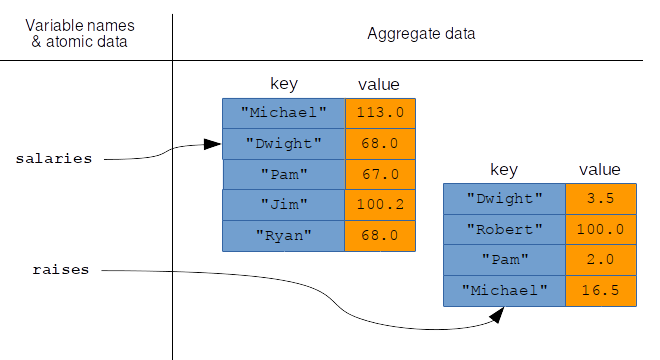
\includegraphics[width=0.9\textwidth]{vectorizedPandas.png}
\caption{Two \texttt{Series}es in memory}
\label{fig:vectorizedPandas}
\end{figure}

Consider the memory picture in Figure~\ref{fig:vectorizedPandas}. Here we have
two \texttt{Series}es, one pointed to by a \texttt{salaries} variable and the
other by \texttt{raises}, which are of different sizes and which have
overlapping, but not identical, sets of keys. What do you suppose Pandas would
do if we executed this code?

\begin{Verbatim}[fontsize=\small,samepage=true,frame=single,framesep=3mm]
new_salaries = salaries + raises
\end{Verbatim}

The answer, happily, is the smartest possible thing it could do. Pandas gets
neither confused nor stifled by the fact that the keys are in different orders
in the two \texttt{Series}es, and instead it does what you surely want:
add corresponding elements, with matching keys, and produce a new
\texttt{Series} with all of those sums.

\begin{figure}[ht]
\centering
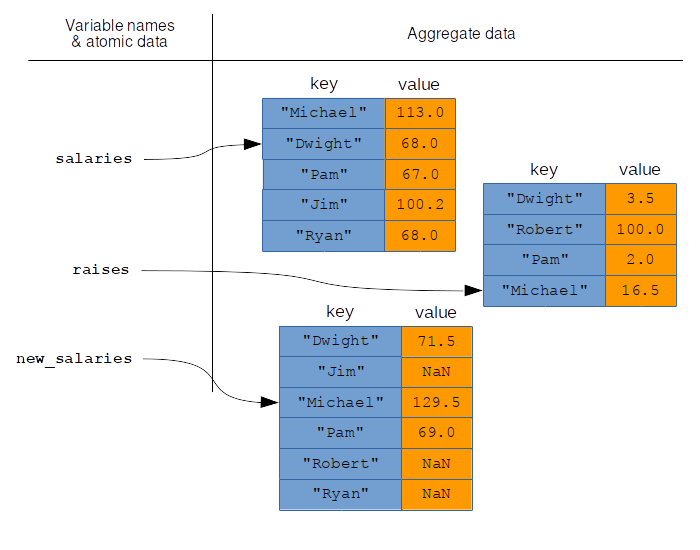
\includegraphics[width=0.8\textwidth]{vectorizedPandas2.png}
\caption{The result of \texttt{+}'ing two \texttt{Series}es that don't have all the same keys.}
\label{fig:vectorizedPandas2}
\end{figure}

The actual result in this case is in Figure~\ref{fig:vectorizedPandas2}, and
the output is here:

% salaries = pd.Series([113,68,67,100.2,68],
%   index=['Michael','Dwight','Pam','Jim','Ryan'])
% raises = pd.Series([3.5,100,2,16.5],
%   index=['Dwight','Robert','Pam','Michael'])

\begin{Verbatim}[fontsize=\small,samepage=true,frame=single,framesep=3mm]
new_salaries = salaries + raises
print(new_salaries)
\end{Verbatim}

\begin{Verbatim}[fontsize=\small,samepage=true,frame=leftline,framesep=5mm,framerule=1mm]
Dwight      71.5
Jim          NaN
Michael    129.5
Pam         69.0
Robert       NaN
Ryan         NaN
dtype: float64
\end{Verbatim}

\index{nan@\texttt{NaN} (``not a number'')}
\index{missing value}

Convince yourself that \texttt{Dwight}'s \$68,000 salary got added to his
\$3,500 raise, and that \texttt{Michael}'s \$113,000 was added to \$16,500,
\textit{etc.}

Don't get freaked out by those \texttt{NaN} entries just yet. The special value
``\textbf{NaN}'' stands for ``\textbf{not a number},'' and basically means that
Pandas has to throw up its hands in that case. And with good cause.
\texttt{Jim} has a current salary of \$100,200 in the first \texttt{Series},
but has no value at all in the second one (no raise for Jim this year? Haven't
decided what his raise will be yet? Something else?) and so Pandas shrugs and
says ``dunno.'' We say that the \texttt{Jim} entry in the
\texttt{new\_salaries} \texttt{Series} is a \textbf{missing value}. The same is
true for \texttt{Robert} and \texttt{Ryan}, each of whom was present in only
one of the two operands.

Now I know what you're thinking: ``can't Pandas just assume the salary and/or
raise is 0 if there's a missing one?'' The answer is that yes it can, but it
won't do so unless you give the go-ahead. Pandas is being cautious here, and
doesn't want to introduce errors into your data stream by false assumptions.
(Maybe in your company, for instance, there's a default entry-level salary that
every employee receives who's unspecified in the \texttt{salary}
\texttt{Series}. Or maybe the yearly raise is always assumed to be a flat 2.5\%
cost-of-living raise unless explicitly specified.)

\index{add@\texttt{add()} function (Pandas)}
\index{sub@\texttt{sub()} function (Pandas)}
\index{mul@\texttt{mul()} function (Pandas)}
\index{div@\texttt{div()} function (Pandas)}

If we do want Pandas to assume a certain default value, we have to change
tactics a bit and go with the \texttt{add()} function (or \texttt{sub()},
\texttt{mul()}, or \texttt{div()}):

\begin{Verbatim}[fontsize=\small,samepage=true,frame=single]
new_salaries = pd.Series.add(salaries, raises, fill_value=0)
print(new_salaries)
\end{Verbatim}

\begin{Verbatim}[fontsize=\small,samepage=true,frame=leftline,framesep=5mm,framerule=1mm]
Dwight      71.5
Jim        100.2
Michael    129.5
Pam         69.0
Robert     100.0
Ryan        68.0
dtype: float64
\end{Verbatim}

The \texttt{fill\_value} argument is the important one here: it specifies what
default value to use if one of the addends is missing a key from the other. Now
the result is as in Figure~\ref{fig:vectorizedPandas3}. You can, of course,
choose a \texttt{fill\_value} other than zero, if you wish.

\begin{figure}[ht]
\centering
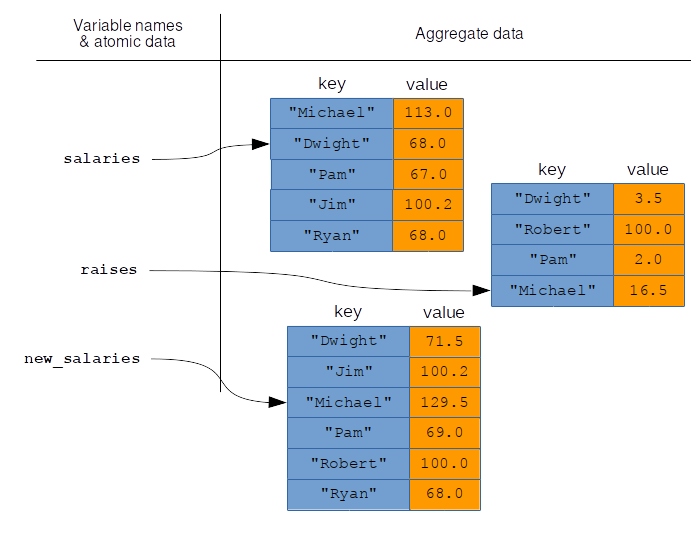
\includegraphics[width=0.8\textwidth]{vectorizedPandas3.png}
\caption{Using \texttt{add()} instead, and passing a \texttt{fill\_value}.}
\label{fig:vectorizedPandas3}
\end{figure}

As with NumPy arrays, we can add (or subtract, or multiply, ...) a single
atomic value to a series as well:

\begin{Verbatim}[fontsize=\small,samepage=true,frame=single,framesep=3mm]
cost_of_living_increase = salaries * .025
print(cost_of_living_increase)
\end{Verbatim}

\begin{Verbatim}[fontsize=\small,samepage=true,frame=leftline,framesep=5mm,framerule=1mm]
Michael    2.825
Dwight     1.700
Pam        1.675
Jim        2.505
Ryan       1.700
dtype: float64
\end{Verbatim}

\begin{Verbatim}[fontsize=\small,samepage=true,frame=single,framesep=3mm]
salaries = salaries + cost_of_living_increase
print(salaries)
\end{Verbatim}

\begin{Verbatim}[fontsize=\small,samepage=true,frame=leftline,framesep=5mm,framerule=1mm]
Michael    115.825
Dwight      69.700
Pam         68.675
Jim        102.705
Ryan        69.700
dtype: float64
\end{Verbatim}

It can sometimes be useful to do string concatenation as well, for instance if
we had employee first names and last names in two \texttt{Series}es with their
employee ID as the index:

\begin{Verbatim}[fontsize=\small,samepage=true,frame=single,framesep=3mm]
firsts = pd.Series(['Hannibal', 'Clarice', 'Multiple', 'Buffalo'],
    index=[666, 1993, 47, 988])
lasts = pd.Series(['Starling', 'Crawford', 'Lecter', 'Bill', 'Miggs'],
    index=[1993, 1650, 666, 988, 47])
print(firsts + " " + lasts)
\end{Verbatim}

\begin{Verbatim}[fontsize=\small,samepage=true,frame=leftline,framesep=5mm,framerule=1mm]
47        Multiple Miggs
666      Hannibal Lecter
988         Buffalo Bill
1650                 NaN
1993    Clarice Starling
dtype: object
\end{Verbatim}

\section{Copying \texttt{Series}es}

\section{Sorting \texttt{Series}es}
\index{in place}

\section{Concatenating and combining}

\section{Queries}

These functions are all summarized in Figure~\ref{fig:handySeries}.

\setlength\extrarowheight{5pt}

\begin{figure}[ht]
\centering
\begin{tabular}{c|p{3.3in}}
Function & Description \\
\hline

\texttt{len(}\textsl{arr}\texttt{)} & Get the number of elements in the array \textsl{arr}. \\

\textsl{arr}\texttt{[17]} & Get a specific element's value from the array \textsl{arr}. \\

\textsl{arr}\texttt{[8] =} (\textsl{something}) & Set a specific element of the array \textsl{arr}. \\

\textsl{arr} \texttt{+ 91} & Add a value to each element of \textsl{arr},
yielding a new array. (Also works with \texttt{-}, \texttt{*}, \texttt{/},
\textit{etc.}) \\

\textsl{arr1} \texttt{+} \textsl{arr2} & Add each pair of values in two arrays,
yielding a new array. (Also works with \texttt{-}, \texttt{*}, \texttt{/},
\textit{etc.}) \\

\textsl{arr1} = \textsl{arr2} & Make \textsl{arr1} point to the same data that
\textsl{arr2} points to. (\textit{Not} a copy!)\\

\textsl{arr1} = \textsl{arr2}\texttt{.copy()} & Make \textsl{arr1} point to a
new, independent copy of \textsl{arr2}. \\

\textsl{arr}\texttt{.sort()} & Sort the array \textsl{arr} \textbf{in place}. (Numerical or
alphabetical, depending on the \texttt{.dtype}.) \\

\texttt{np.sort(}\textsl{arr}) & Return a new array with the sorted elements
of \textsl{arr}. (Numerical or alphabetical, depending on the \texttt{.dtype}.)
\\

\texttt{np.append(}\textsl{arr}, \textsl{elem}\texttt{)} &
    Return a new array with \textsl{elem} tacked on to the end. \\

\texttt{np.append(}\textsl{arr1}, \textsl{arr2}\texttt{)} &
    Return a new array with the two arrays \textsl{arr1} and \textsl{arr2} concatenated. \\

\texttt{np.insert(}\textsl{arr}, \textsl{ind}, \textsl{val}\texttt{)} &
    Return a new array with the new value \textsl{val} inserted into position \textsl{ind} of \textsl{arr}. \\

\texttt{np.delete(}\textsl{arr}, \textsl{ind}\texttt{)} &
    Return a new array with the element at index \textsl{ind} removed from \textsl{arr}. \\

\texttt{np.flip(}\textsl{arr}\texttt{)} &
    Return a new array with \textsl{arr} in reverse order. \\
\end{tabular}
\bigskip
\caption{Handy functions, methods, and operators for Pandas \texttt{Series}es.}
\label{fig:handySeries}
\end{figure}


\chapter[Associative arrays in Python (3 of 3)]{\huge\selectfont{Associative
arrays in Python (3 of 3)}}
\label{ch:assocArraysInPython3}

\index{min@\texttt{.min()} (Pandas)}
\index{max@\texttt{.max()} (Pandas)}
\index{idxmin@\texttt{.idxmin()} (Pandas)}
\index{idxmax@\texttt{.idxmin()} (Pandas)}
\index{index@index (pl:~indices)}
\index{key-value pair}

But wait, there's more! We can also use methods like \texttt{.min()},
\texttt{.max()}, \texttt{.idxmin()}, and \texttt{.idxmax()} to get the
``extremes'' of a \texttt{Series} -- \textit{i.e.} the lowest and highest
values in a \texttt{Series}, or their keys (indexes). Note that
\texttt{.idxmin()} does \textit{not} give you the lowest key in the
\texttt{Series}! Instead, it gives you \textit{the key of the lowest value}.
Study this code snippet and its output to test your understanding of this:

\index{understanding@\texttt{understanding}}

\begin{Verbatim}[fontsize=\small,samepage=true,frame=single,framesep=3mm]
understanding = pd.Series([15,4,13,3,7], index=[4,10,2,12,9])
print(understanding)
print("The min is {}.".format(understanding.min()))
print("The max is {}.".format(understanding.max()))
print("The idxmin is {}.".format(understanding.idxmin()))
print("The idxmax is {}.".format(understanding.idxmax()))
\end{Verbatim}

\begin{Verbatim}[fontsize=\small,samepage=true,frame=leftline,framesep=5mm,framerule=1mm]
4     15
10     4
2     13
12     3
9      7
dtype: int64

The min is 3.
The max is 15.
The idxmin is 12.
The idxmax is 4.
\end{Verbatim}

The \texttt{idxmin} and \texttt{idxmax} are \texttt{12} and \texttt{4},
respectively, since the smallest value in the series (the \texttt{3}) has a key
of \texttt{12}, and the largest value (the \texttt{15}) has a key of
\texttt{4}.

\index{index@\texttt{.index} syntax (Pandas)}

If we did actually want the lowest (or highest) key, we could use the
\texttt{.index} syntax (see p.~\pageref{dotIndex}) to achieve that:

\begin{Verbatim}[fontsize=\small,samepage=true,frame=single,framesep=3mm]
print("The lowest key is {}.".format(understanding.index.min()))
print("The highest key is {}.".format(understanding.index.max()))
\end{Verbatim}

\begin{Verbatim}[fontsize=\small,samepage=true,frame=leftline,framesep=5mm,framerule=1mm]
The lowest key is 2.
The highest key is 12.
\end{Verbatim}

And remember that ``lowest''/``highest'' for string data means alphabetical
order.

\section{Queries}

\index{query}
\index{match (a query)}
\index{filter}

One of the most powerful things we'll do with a data set is to \textbf{query}
it. This means that instead of specifying (say) a particular key, or something
like ``the minimum'' or ``the maximum,'' we provide our own custom criteria and
ask Pandas to give us all values that \textbf{match}. This kind of operation is
also sometimes called \textbf{filtering}, because we're taking a long list of
items and sifting out only the ones we want.

\index{boxies (square brackets)}
\index{[]@\texttt{[]} (boxies)}

\index{condition (of a query)}

The syntax is interesting: you still use the boxies (like you do when
giving a specific key) but inside the boxies you put a \textbf{condition} that
will be used to select elements. It's best seen with an example. Re-using the
\texttt{understanding} variable from above, we can query it and ask for all the
elements greater than 5:

\begin{Verbatim}[fontsize=\small,samepage=true,frame=single,framesep=3mm]
more_than_five = understanding[understanding > 5]
print(more_than_five)
\end{Verbatim}

\begin{Verbatim}[fontsize=\small,samepage=true,frame=leftline,framesep=5mm,framerule=1mm]
4    15
2    13
9     7
dtype: int64
\end{Verbatim}

The new thing here is the ``\texttt{understanding > 5}'' thing inside the
boxies. The result of this query is itself a \texttt{Series}, but one in which
everything that doesn't match the condition is filtered out. Thus we only have
three elements instead of five. Notice the keys didn't change, and they also
had nothing to do with the query: our query was about \textit{values}.

\index{index@\texttt{.index} syntax (Pandas)}

We could change this, if we were interested in putting a restriction on
\textit{keys} instead, using the \texttt{.index} syntax:

\begin{Verbatim}[fontsize=\small,samepage=true,frame=single,framesep=3mm]
index_more_than_five = understanding[understanding.index > 5]
print(index_more_than_five)
\end{Verbatim}

\begin{Verbatim}[fontsize=\small,samepage=true,frame=leftline,framesep=5mm,framerule=1mm]
10    4
12    3
9     7
dtype: int64
\end{Verbatim}

See how tacking on ``\texttt{.index}'' in the query made all the difference.

\subsection{Query operators}

\index{wakkas (angle brackets)}
\index{<>@\texttt{<>} (wakkas)}

Now I have a surprise for you. It makes perfect sense to use the character
``\texttt{>}'' (called ``greater-than,'' ''right-angle-bracket,'' or simply
''wakka'') to mean ``greater than.'' And the character ``\texttt{<}'' makes
sense as ``less than.'' Unfortunately, the others don't make quite as much
sense. See the top table in Figure~\ref{fig:queryOps}.

\index{bang (``\texttt{"!}'')}
\index{"!@\texttt{"!} (bang)}
\index{bang-equals (``\texttt{"!=}'')}

``Greater/less than or equal to'' isn't hard to remember, and it's a good thing
Python doesn't require symbols like ``$\le$'' or ``$\ge$'' since those are hard
to find on your keyboard. You just type both symbols back-to-back, with no
space. More problematic are the last two entries in the top table. The
``\texttt{!=}'' operator (pronounced ``bang-equals'') is used as a stand-in
for ``$\ne$'' which also isn't keyboard friendly. And that one doesn't have a
good mnemonic; you just have to memorize it.

\index{double-equals (\texttt{==})}
\index{==@\texttt{==} (double-equals)}

By far the most error-prone of this set is the ``\texttt{==}''
(\textbf{double-equals}) operator, which simply means ``equals.'' \textbf{Yes,
you do have to use double-equals instead of single-equals in your queries, and
yes it matters.} As additional incentive, let me inform you that if you use
single-equals when you needed to use double-equals, \textit{it will seem to
work at first}, but you will silently get the wrong answer.

\textbf{Memorize this fact!} Failing to use double-equals is quite possibly the
single most common programming error for beginners.

\begin{figure}[ht]
\centering
\small
\bigskip
\underline{\textit{Simple query operators:}}\\
\smallskip
\begin{tabular}{c|c}
Symbol & Meaning \\
\hline
\texttt{>} & greater than \\
\hline
\texttt{<} & less than \\
\hline
\texttt{>=} & greater than or equal to \\
\hline
\texttt{<=} & less than or equal to \\
\hline
\texttt{!=} & \textit{not} equal to \\
\hline
\texttt{==} & equal to \\
\end{tabular}

\bigskip
\bigskip
\underline{\textit{Compound query operators:}}\\
\smallskip
\begin{tabular}{c|c}
Symbol & Meaning \\
\hline
\texttt{\&} & and \\
\hline
\texttt{|} & or \\
\hline
\texttt{\textasciitilde} & not \\
\end{tabular}

\bigskip
\normalsize
\caption{Query operators: simple and compound}
\label{fig:queryOps}
\end{figure}


Here are some more examples to test your understanding. Make sure you
understand why each output is what it is.

\begin{Verbatim}[fontsize=\small,samepage=true,frame=single,framesep=3mm]
understanding = pd.Series([15,4,13,3,7], index=[4,10,2,12,9])
print(understanding[understanding <= 7])
\end{Verbatim}
\vspace{-.3in}

\begin{Verbatim}[fontsize=\small,samepage=true,frame=leftline,framesep=5mm,framerule=1mm]
10    4
12    3
9     7
dtype: int64
\end{Verbatim}

\begin{Verbatim}[fontsize=\small,samepage=true,frame=single,framesep=3mm]
print(understanding[understanding != 13])
\end{Verbatim}
\vspace{-.3in}

\begin{Verbatim}[fontsize=\small,samepage=true,frame=leftline,framesep=5mm,framerule=1mm]
4     15
10     4
12     3
9      7
dtype: int64
\end{Verbatim}

\begin{Verbatim}[fontsize=\small,samepage=true,frame=single,framesep=3mm]
print(understanding[understanding == 3])
\end{Verbatim}
\vspace{-.3in}

\begin{Verbatim}[fontsize=\small,samepage=true,frame=leftline,framesep=5mm,framerule=1mm]
12    3
dtype: int64
\end{Verbatim}

\begin{Verbatim}[fontsize=\small,samepage=true,frame=single,framesep=3mm]
print(understanding[understanding.index >= 9])
\end{Verbatim}
\vspace{-.3in}

\begin{Verbatim}[fontsize=\small,samepage=true,frame=leftline,framesep=5mm,framerule=1mm]
10    4
12    3
9     7
dtype: int64
dtype: int64
\end{Verbatim}


\subsection{Compound queries}

\index{compound condition}

Often, your query will involve more than one criterion. This is called a
\textbf{compound condition}. It's not as common with \texttt{Series}es as it
will be with \texttt{DataFrame}s in a couple chapters, but there are still uses
for it here.

\index{and (compound condition)}

Suppose I want all the key/value pairs of \texttt{understanding} where the
value is \textit{between 5 and 14}. This is really two conditions masquerading
as one: we want all pairs where (1) the value is greater than 5, \textbf{and}
also (2) the value is less than 14. I put the word ``\textbf{and}'' in boldface
in the previous sentence because that's the operator called for here. We only
want elements in our results where \textit{both} things are true, and
therefore, we ``\textit{and} together the two conditions.'' (``And'' is being
used as a verb here.)

The way to achieve this is as follows. The syntax is nutty, so pay close
attention:

\begin{Verbatim}[fontsize=\small,samepage=true,frame=single,framesep=3mm]
betw_5_and_14 = understanding[(understanding > 5) & (understanding < 14)]
print(betw_5_and_14)
\end{Verbatim}

\begin{Verbatim}[fontsize=\small,samepage=true,frame=leftline,framesep=5mm,framerule=1mm]
2    13
9     7
dtype: int64
\end{Verbatim}

First, notice that we put each of our two conditions \textit{in bananas} here.
This is \textit{not} optional, as it turns out: you'll get a non-obvious error
message if you omit them. Second, see how we combined the two with the
``\texttt{\&}'' operator from the bottom half of Figure~\ref{fig:queryOps}. The
result, then, was only the elements that satisfied \textit{both} conditions.

\index{or (compound condition)}
\index{pipe (vertical bar, or ``\texttt{|}'')}
\index{|@\texttt{|} (pipe)}

It can be tricky to figure out whether you want an \textbf{and} or an
\textbf{or}. Unfortunately they don't always correspond to their colloquial
English usage. Let's see what happens if we switch the ``\texttt{\&}'' symbol to
a ``\texttt{|}'' (pronounced ``pipe''):

\begin{Verbatim}[fontsize=\small,samepage=true,frame=single,framesep=3mm]
different_ex = understanding[(understanding > 5) | (understanding < 14)]
print(different_ex)
\end{Verbatim}

\begin{Verbatim}[fontsize=\small,samepage=true,frame=leftline,framesep=5mm,framerule=1mm]
4     15
10     4
2     13
12     3
9      7
dtype: int64
\end{Verbatim}

You can see that we got everything back. That's because \textbf{or} means
``only give me the elements where \textit{either one} of the conditions,
\textit{or both}, are true.'' In this case, this is guaranteed to match
everything, because if you think about it, \textit{every} number is either
greater than five, or less than fourteen, or both. (Think deeply.)

Even though in this example it didn't do anything exciting, an ``\textbf{or}''
does sometimes return a useful result. Consider this example:

\begin{Verbatim}[fontsize=\small,samepage=true,frame=single,framesep=3mm]
useful = understanding[(understanding.index > 10) | (understanding > 5)]
print(useful)
\end{Verbatim}

\begin{Verbatim}[fontsize=\small,samepage=true,frame=leftline,framesep=5mm,framerule=1mm]
4     15
2     13
12     3
dtype: int64
\end{Verbatim}

Here we're asking for all key/value pairs in which \textit{either} the key is
greater than ten, \textit{or} the value is greater than ten, or both. This
reeled in exactly three fish as shown above. If we changed this ``\texttt{|}''
to an ``\texttt{\&}'', we'd have caught \textit{no} fish. (Take a moment to
convince yourself of that.)

\index{not (query condition)}
\index{squiggle (tilde, or ``\texttt{\textasciitilde}'')}
\index{~@\texttt{\textasciitilde} (squiggle)}

The last entry in Figure~\ref{fig:queryOps} is the ``\texttt{\textasciitilde}''
sign, which is pronounced ``tilde,'' ``twiddle,'' or ``squiggle.'' It
corresponds to the English word \textbf{not}, although in an unusual place in
the sentence. Here's an example:

\begin{Verbatim}[fontsize=\small,samepage=true,frame=single,framesep=3mm]
ex = understanding[~(understanding.index > 10) | (understanding > 10)]
print(ex)
\end{Verbatim}

\begin{Verbatim}[fontsize=\small,samepage=true,frame=leftline,framesep=5mm,framerule=1mm]
4     15
10     4
2     13
9      7
dtype: int64
\end{Verbatim}

Search for and stare at the squiggle in that line of code. In English, what we
said was ``give me elements where either the key is \textit{not} greater than
ten, or the value is greater than ten, or both.'' The four matching elements
are shown above. 

Changing the ``or'' back to an ``and'' here gives us this output instead:

\begin{Verbatim}[fontsize=\small,samepage=true,frame=single,framesep=3mm]
ex2 = understanding[~(understanding.index > 10) | (understanding > 10)]
print(ex2)
\end{Verbatim}

\begin{Verbatim}[fontsize=\small,samepage=true,frame=leftline,framesep=5mm,framerule=1mm]
4     15
2     13
dtype: int64
\end{Verbatim}

These are the only two rows where \textit{both} conditions are true (and
remember that the first one is not-ted.)

It can be tricky to get your queries right. As with most things, it just takes
some practice.

\subsection{Queries on strings}

% pronounce "where" instead of "of"

\subsubsection{Common pitfalls}

A couple things before we move on. You've noticed that in all the above
examples, it was necessary to type the word \texttt{understanding}
\textit{twice}: once to specify the \texttt{Series} to query, and once as pat
of the query itself. There's no way around that, sorry; you just have to get
used to it.



\chapter{Loops}
\label{ch:loops}

\index{non-linear}
\index{loop}

It's time for our first look at a \textbf{non-linear} program. Up to now, all
of our Python programs have executed step-by-step, start to finish, like a
metronome, with each line of code getting executed exactly once. That's about
to change. In this chapter, we introduce the concept of a \textbf{loop}, which
is a programming construct that directs lines of code to be executed
\textit{repeatedly}, and out of strict sequence.

\section{The two species of loops}

\index{fixed-iteration (loop)}
\index{variable-iteration (loop)}
\index{counter-controlled (loop)}
\index{condition-controlled (loop)}
\index{for loop@\texttt{for} loop}
\index{while loop@\texttt{while} loop}

Although some programming languages try to dress them up further, there are
really only two fundamental kinds of loops in the world:
\textbf{fixed-iteration loops} and \textbf{variable-iteration
loops}.\footnote{Sometimes these are called \textbf{counter-controlled} and
\textbf{condition-controlled} loops, respectively.} The first kind is simpler
to understand and less error-prone; in most languages (Python included) it is
implemented as a ``\textbf{\texttt{for} loop}.'' The tricker, second kind is
available to programmers as a ``\textbf{\texttt{while} loop}.''

Happily for us, it turns out that \texttt{while} loops don't come up much in
Data Science, at least in the beginning. There are some more advanced
techniques that use them (for instance, optimization methods and threshold
detection) but for us it's going to be \texttt{for} loops that dominate the
landscape. So let's figure out how they work.

\section{A word of caution}

\index{query}

But before we embark, a cautionary note. Some of the things that loops can do
-- especially the early examples -- can also be done using the queries of the
last chapter. For instance, we could use a query to find all the strings in a
\texttt{Series} that begin with the letter \texttt{T}, or we could use a loop
to do the same thing.

Here's the rule: \textbf{if you can do it without a loop, that is always
preferred.} There are two reasons for this. First, it's less code to write, and
less error-prone, to use Pandas' built-in features rather than crafting a loop
yourself. That's why they created those features (like queries) after all.

Second, and ultimately even more important, using a Pandas function is
\textit{much faster} to execute than a loop. The reason has to do with how a
loop is eventually broken down into the little instructions a machine can
understand: when Python runs a loop, it plods through the steps methodically,
whereas the Pandas functions are all pre-baked into a water-cooled rocket
engine that can jet out of the gate.

You don't need to know any of those nitty-gritty details. All you have to
remember is: don't ever resort to using a loop unless you can't figure out how
to do what you want without one. (And unfortunately, there are indeed those
times.)

\section{Iterating through an array}

\index{iterate}

Most often, we'll use a \texttt{for} loop to ``loop through,'' or
``\textbf{iterate} through,'' the contents of an aggregate data variable. This
means that instead of executing a snippet of code \textit{once}, we'll execute
it \textit{once per element of the variable}. This ``once per element'' thing
is what makes the code non-linear.

\index{array}
\index{ndarray@\texttt{ndarray} (NumPy)}

Let's start with the first aggregate data type we learned, a NumPy array.

\begin{Verbatim}[fontsize=\small,samepage=true,frame=single,framesep=3mm]
 1: villains = np.array(['Jafar','Ursula','Maleficent','Gaston'])
 2: print("Here we go!")
 3: for villain in villains:
 4:     print("Oooo, {} is scary!".format(villain))
 5:     print("({} has {} letters.)".format(villain, len(villain)))
 6: print("Whew!")
\end{Verbatim}

\index{loop!header}
\index{loop!body}

(I've numbered the lines in this example so I can refer to them in the text
below, but the numbers and colons aren't part of Python.)

Immediately after creating our \texttt{villains} array, and printing an
introductory message, we encounter our first loop. A loop consists of two
parts: the \textbf{loop header} and the \textbf{loop body}. Here are the rules:

\index{indentation}
\index{curlies (curly braces)}
\index{\{\}@\texttt{\{\}} (curlies)}

\begin{compactitem}
\item The loop header consists of the line that begins with ``\texttt{for}''.
\item The loop body consists of \textit{all of the consecutive following lines
that are \textbf{indented} (tabbed-over) one tab.}\footnote{Other programming
languages -- every other one I know besides Python, in fact -- uses some other
way to designate the loop body than indentation. Many (R and Java, for
instance) use curly braces before and after the loop body so that the computer
knows where it begins and ends. I personally like this feature of Python's, but
there are haters, and the bottom line is you just have to get used to it.}
\end{compactitem}

That second rule turns out to be more important than it seems at first. A very
(\textit{very!}) common error among beginners is to ``mis-indent'' their code
such that their loop body includes more, or less, than they mean it to. So
heads up.

Before we continue, stare at that code above and convince yourself of these two
facts:

\begin{compactitem}
\item[\leftpointright] The loop header is line \textbf{3}.
\item[\leftpointright] The loop body is lines \textbf{4 and 5}. (\textit{Not} line 4
only! \textit{Not} lines 4, 5, and 6!)
\end{compactitem}

\medskip
Now the reason this is important is that a \texttt{for} loop works as follows:
\vspace{-.1in}

\index{memory picture}

\definecolor{shadecolor}{rgb}{.9,.9,.9}
\begin{shaded}
\begin{compactenum}
\itemsep.1em
\item First, create a new variable (on the left-hand side of the memory
picture) named whatever comes immediately after the word ``\texttt{for}''. (In
this example, the name of this new variable will be \texttt{villain}.)
\item Then, for \textit{each} element of the array, in succession:
    \begin{compactenum}
    \itemsep.1em
    \item Set that variable's value to the next element of the array.
    \item \textit{Execute the entire loop body.} (In this example, lines 4--5.)
    \end{compactenum}
\end{compactenum}
\end{shaded}

In the \texttt{villains} example, therefore, the lines in order of execution
are:

\begin{center}
1, 2, 3, 4, 5, 3, 4, 5, 3, 4, 5, 3, 4, 5, 6.
\end{center}

(Do you agree?)

The memory picture changes constantly throughout any program, including those
that contain loops. Let's take a snapshot of memory as it appears immediately
after executing line 3 the \textit{second} time. In other words, we'll run the
program this far before hitting the pause button:

\begin{center}
1, 2, 3, 4, 5, 3, \textit{Freeze!!}
\end{center}

\index{loop variable}

Memory at this instant is depicted in Figure~\ref{fig:loopsMemory}. The second
time we executed line 3, we set \texttt{villain} (sometimes called the
\textbf{loop variable}, by the way) to the second element of the array,
\texttt{"Ursula"}. We're just about to execute line 4 for the second time. Note
that the \texttt{villains} array is unaffected by this entire loop process:
only our temporary, made-up loop variable (\texttt{villain}) gets a new value
each time.

\begin{figure}[ht]
\centering
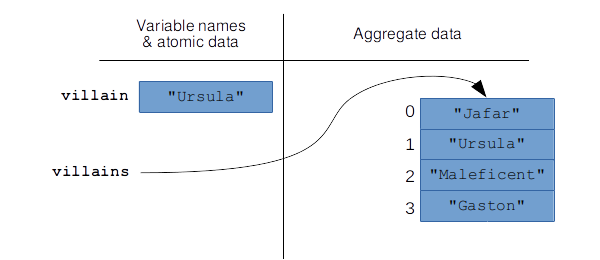
\includegraphics[width=0.8\textwidth]{loopsMemory.png}
\caption{A snapshot of memory immediately after the \textit{second} execution
of line \textit{3} of the \texttt{villains} program.}
\label{fig:loopsMemory}
\end{figure}

The complete output of the program, as you can easily deduce, is thus:

\begin{Verbatim}[fontsize=\small,samepage=true,frame=leftline,framesep=5mm,framerule=1mm]
Here we go!
Oooo, Jafar is scary!
(Jafar has 5 letters.)
Oooo, Ursula is scary!
(Ursula has 6 letters.)
Oooo, Maleficent is scary!
(Maleficent has 10 letters.)
Oooo, Gaston is scary!
(Gaston has 6 letters.)
Whew!
\end{Verbatim}

Don't miss the fact that the ``\texttt{scary!}''~and ``\texttt{has $n$
letters}'' messages were printed four times each, whereas
``\texttt{Whew!}''~only appeared once. That has everything to do with the
indentation: it told Python that lines 4 and 5 \textit{were} part of the loop
body, whereas line 6 was just ``business as usual,'' taking place only after
all the loop hoopla was over and done with.

\section{Iterating through the values of a \texttt{Series}}

\index{iteration}

Great news: if you mastered the previous section, this one and the next will be
a snap. That's because Python, NumPy, and Pandas work together to make
iterating through a \texttt{Series} pretty much \textit{exactly the same} as
iterating through an array. In fact, sometimes you're not even sure which type
you've got!

\index{Marvel comics}

Here's the Marvel \texttt{Series} regurgitated yet again:

\begin{Verbatim}[fontsize=\small,samepage=true,frame=single,framesep=3mm]
alter_egos = pd.Series(['Hulk','Spidey','Iron Man','Thor'],
    index=['Bruce','Peter','Tony','Thor'])
\end{Verbatim}

\index{Thanos}
\index{snap@``the snap''}

Let's say I want to go through and greet all our heroes. It's a snap! (no pun
intended):

\begin{Verbatim}[fontsize=\small,samepage=true,frame=single,framesep=3mm]
print("Welcome to the Marvel Cinematic Universe(tm).")
for hero in alter_egos:
    print("Greetings, {}!".format(hero))
print("Go team!")
\end{Verbatim}

\begin{Verbatim}[fontsize=\small,samepage=true,frame=leftline,framesep=5mm,framerule=1mm]
Welcome to the Marvel Cinematic Universe(tm).
Greetings, Hulk!
Greetings, Spidey!
Greetings, Iron Man!
Greetings, Thor!
Go team!
\end{Verbatim}

What could be easier?

Notice that ``looping through the \texttt{Series}'' effectively means ``looping
through the \textit{values} of the \texttt{Series},'' not the keys. What if we
want to loop through the keys instead?

\section{Iterating through the keys of a \texttt{Series}}

\index{iteration}
\index{index@\texttt{.index} syntax (Pandas)}

I'm glad you asked. But in fact, you already know the answer: just use the
\texttt{.index} syntax from p.~\pageref{dotIndex}!

\begin{Verbatim}[fontsize=\small,samepage=true,frame=single,framesep=3mm]
print("Let's iterate through the keys instead:")
for secret_identity in alter_egos.index:
    print("Nice to meet you, {}.".format(secret_identity))
print("Carry on...")
\end{Verbatim}

\begin{Verbatim}[fontsize=\small,samepage=true,frame=leftline,framesep=5mm,framerule=1mm]
Let's iterate through the keys instead:
Nice to meet you, Bruce.
Nice to meet you, Peter.
Nice to meet you, Tony.
Nice to meet you, Thor.
Carry on...
\end{Verbatim}

\index{loop variable}

By the way, you can see that the name of the loop variable is completely at
your discretion. I called the previous one ``\texttt{hero}'' and this one
``\texttt{secret\_identity}'' just because those names were reflective of their
contents. But it's really up to you: it has nothing to do with the name of the
\texttt{Series} itself. (Yeah, I know the Marvel identities aren't secret
anymore, but I'm old school.)

\section{Iterating through the keys \textit{and} values of a \texttt{Series}}

\index{items@\texttt{.items()} (Pandas)}

Finally, it's common to need access to both halves of each key/value pair as
you iterate through a \texttt{Series}. The way to accomplish this is to call
the \texttt{.items()} method of the \texttt{Series}. But it's tricky, because
when you use \texttt{.items()} you assign \textit{two} variables in your loop
instead of just one.

Before showing the complete loop, let's focus on just the loop header needed
for this technique:

\begin{Verbatim}[fontsize=\normalsize,samepage=true,frame=single,framesep=3mm]
for secret_identity, hero in alter_egos.items():
\end{Verbatim}

I named two loop variables, separated by a comma. The reason I put
\texttt{secret\_identity} first is that in this \texttt{Series}, we used
\texttt{Bruce}, \texttt{Peter}, \textit{etc.} as the \textit{keys}, with the
superhero names as the values. And with \texttt{.items()}, the variable name
you want to use for the key is listed first.

The rest of the loop follows logically from this, with both variables available
inside the loop body:

\begin{Verbatim}[fontsize=\small,samepage=true,frame=single,framesep=3mm]
print("We're now going to recognize some outstanding citizens.")
for secret_identity, hero in alter_egos.items():
    print("{}, known to his friends as {}.".format(hero, secret_identity))
    print("The crowd screams: 'YAY {}!'".format(hero.upper()))
print("Thanks, everyone, for your service.")
\end{Verbatim}

If we freeze the program just after the \textit{third} execution of the loop
header this time, we get the picture in Figure~\ref{fig:loopsMemory2}. And the
output, of course, is:

\begin{Verbatim}[fontsize=\small,samepage=true,frame=leftline,framesep=5mm,framerule=1mm]
We're now going to recognize some outstanding citizens.
Hulk, known to his friends as Bruce.
The crowd screams: 'YAY HULK!'
Spidey, known to his friends as Peter.
The crowd screams: 'YAY SPIDEY!'
Iron Man, known to his friends as Tony.
The crowd screams: 'YAY IRON MAN!'
Thor, known to his friends as Thor.
The crowd screams: 'YAY THOR!'
Thanks, everyone, for your service.
\end{Verbatim}

\begin{figure}[ht]
\centering
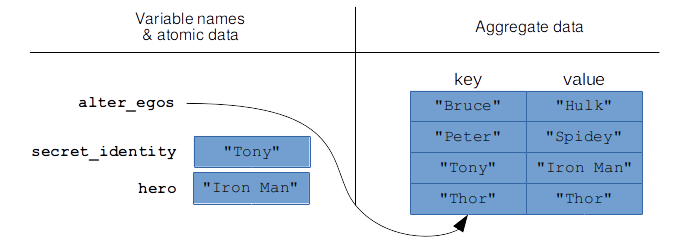
\includegraphics[width=0.9\textwidth]{loopsMemory2.png}
\caption{A snapshot of memory immediately after the \textit{third} execution
of the loop header in the \texttt{alter\_egos} program.}
\label{fig:loopsMemory2}
\end{figure}

\section{Wrapping up}

We can, of course, do much more inside loops than just print things. We can
perform computations galore. The examples in this chapter were simply to
illustrate the structure and behavior of \texttt{for} loops, so that you have a
framework for understanding how more complex parts fit into them later.

Onward!


\chapter[EDA: univariate]{Exploratory Data Analysis: univariate}
\label{ch:edaUnivariate}

\index{Exploratory Data Analysis (EDA)}

The fancy term ``\textbf{Exploratory Data Analysis}'' (EDA) basically just
means getting acquainted with your data. After importing a new data set into
Python, the first thing you normally do is poke around to get an idea of what
it contains. You may not even know what questions you eventually want to ask --
let alone what the answers are -- but sizing up the data is a necessary
precursor to those activities.

\index{univariate}

In this chapter, we'll learn some basic EDA techniques for \textbf{univariate
data}, which is really all we've studied so far. ``Univariate'' means to
consider just one variable at a time, rather than possible relationships
between variables. A single (one-dimensional) NumPy array or Pandas
\texttt{Series} is a univariate data set, if you treat it in isolation. As it
turns out, there's quite a few interesting things you can do with even
something that simple.

\index{summary statistics}

\index{scales of measure}
\index{categorical variable}
\index{nominal variable}

First, we'll look at \textbf{summary statistics}, which are a way to capture
the general features of a data set so you can see the forest instead of just a
bunch of trees. Which type of summary information is appropriate depends on
whether you're dealing with categorical or numeric data.

\section[Categorical: counts of occurrences]{Categorical data: counts of occurrences}

\label{categoricalDataValueCounts}

\index{faves@\texttt{faves}}
\index{Swift@Swift, Taylor}
\index{Perry@Perry, Katy}

Let's say you had access to a poll on people's favorite pop stars. You import
this into a big ol' Pandas \texttt{Series} called \texttt{faves}:

\begin{Verbatim}[fontsize=\scriptsize,samepage=true,frame=single,framesep=3mm]
print(faves)
\end{Verbatim}

\begin{Verbatim}[fontsize=\scriptsize,samepage=true,frame=leftline,framesep=5mm,framerule=1mm]
0          Katy Perry
1             Rihanna
2       Justin Bieber
3               Drake
4             Rihanna
5        Taylor Swift
6               Adele
7               Adele
8        Taylor Swift
9       Justin Bieber
...
1395       Katy Perry
dtype: object
\end{Verbatim}

\index{value\_counts@\texttt{.value\_counts()} method (Pandas)}

That's great, but it's also kinda TMI. You probably don't care who the
\textit{first} person's idol is, nor the fifteenth, nor the last. Much more
interesting is simply \textit{how many times} each value appears in the
\texttt{Series}. This information is available from the Pandas
\texttt{.value\_counts()} method:

\begin{Verbatim}[fontsize=\small,samepage=true,frame=single,framesep=3mm]
counts = faves.value_counts()
print(counts)
\end{Verbatim}

\begin{Verbatim}[fontsize=\small,samepage=true,frame=leftline,framesep=5mm,framerule=1mm]
Taylor Swift     388
Katy Perry       265
Drake            261
Adele            212
Rihanna          136
Justin Bieber    134
dtype: int64
\end{Verbatim}

The \texttt{.value\_counts()} method returns another \texttt{Series}, but the
\textit{values} of the original \texttt{Series} become the \textit{keys} of the
new one. This tells us at a glance how popular each answer is relative to the
others.

To get percentages instead of totals, just divide by the total and multiply by
100, of course:

\begin{Verbatim}[fontsize=\small,samepage=true,frame=single,framesep=3mm]
print(counts / len(counts) * 100)
\end{Verbatim}

\begin{Verbatim}[fontsize=\small,samepage=true,frame=leftline,framesep=5mm,framerule=1mm]
Taylor Swift     0.277937
Katy Perry       0.189828
Drake            0.186963
Adele            0.151862
Rihanna          0.097421
Justin Bieber    0.095989
dtype: float64
\end{Verbatim}

\index{mode}
\index{central tendency}
\index{measure of central tendency}

Recall (p.~\pageref{mode}) that the \textbf{mode} is the only measure of
central tendency that makes sense for categorical data. And all you have to do
is call \texttt{.value\_counts()} and look at the top result. (In this case,
\texttt{Taylor Swift}.)

Note that \texttt{.value\_counts()} is a Pandas \texttt{Series} method, not a
NumPy method. If you find yourself with a NumPy array instead, you can just
\textbf{wrap} it in a \texttt{Series} as we did in Section~\ref{wrap}
(p.~\pageref{wrap}):

\begin{Verbatim}[fontsize=\small,samepage=true,frame=single,framesep=3mm]
my_array = np.array(['red','blue','red','green','green',
    'green','blue'])
print(pd.Series(my_array).value_counts())
\end{Verbatim}

\begin{Verbatim}[fontsize=\small,samepage=true,frame=leftline,framesep=5mm,framerule=1mm]
green    3
red      2
blue     2
dtype: int64
\end{Verbatim}

\section{Numerical data: quantiles}

\label{quantiles}
\index{real number}
\index{quantile}
\index{cut point (quantile)}

A \textbf{quantile} is a real number between 0 and 1 that represents a
``\textbf{cut point}'' of a numerical data set: roughly speaking, it's the
number for which a certain fraction of the values are \textit{less than} that
number. So the ``.2-quantile'' (pronounced ``point two quantile'') of a
variable containing the heights of third-graders might be 50 inches. If that's
the case, it would indicate that \textit{20\% of the third-graders are less
than 50 inches tall.}

Quantiles are very revealing, but underappreciated. Most people don't seem to
know how to interpret them. But once you figure it out, you'll realize that
quantiles tell you almost everything possible to know about a numeric variable:
by dialing the quantile between 0 and 1, you can tell exactly how common values
in a certain range are.

\index{quantile@\texttt{.quantile()} method (Pandas)}

In Python, you simply call the \texttt{.quantile()} method on a
\texttt{Series}, passing a number between 0 and 1 as an argument, and it tells
you exactly where that cut point is.

Now there's a little bit of weirdness around the edges, depending on the exact
definition used to calculate the quantiles. Let's say I collected some salary
data, and got these responses (``k'' means ``thousand dollars per year,'' and
``M'' means ``million dollars per year''):

\begin{center}
35k\quad 22k\quad 67k\quad 45k\quad 35k\quad 8M\quad 94k\quad 51k\quad 53k\quad
64k\quad 54k
\end{center}

How would I calculate, say, the .7-quantile? First, sort the numbers:

\begin{center}
22k\quad 35k\quad 35k\quad 45k\quad 51k\quad 53k\quad 54k\quad 64k\quad 67k\quad 94k\quad 8M
\end{center}

(yes, we \textit{do} include the 35k value twice; don't eliminate duplicates)
and then spread out the quantiles ``evenly'' from 0 to 1:

\begin{center}
\scriptsize
\renewcommand{\arraystretch}{.7}
\begin{tabular}{rccccccccccc}
value: & 22k& 35k& 35k& 45k& 51k& 53k& 54k& 64k& 67k& 94k& 8M\\
& $\uparrow$ &
$\uparrow$ &
$\uparrow$ &
$\uparrow$ &
$\uparrow$ &
$\uparrow$ &
$\uparrow$ &
$\uparrow$ &
$\uparrow$ &
$\uparrow$ &
$\uparrow$ \\
quantile: & .0\ \ & .1\ \  & .2\ \  & .3\ \  & .4\ \  & .5\ \  & .6\ \  & .7\ \  & .8\ \  & .9\ \  & 1.0 \\
\end{tabular}
\end{center}

Don't get picky on me. If you were picky, you could quibble at saying ``the
.3-quantile is 45k'' since it's technically \textit{not} true that 30\% of the
values are less than 45k: in truth, 3 out of 11 (27.3\%) of them are. Whatever,
whatever. The point is that 45k is at the ``cut point'' that's
$\frac{3}{10}$ths of the way through the values from min to max. Quantiles
aren't about laser precision anyway: they're about understanding the general
pattern of the data.

\subsection{``Special'' quantiles}

\index{median}

You'll realize as an immediate consequence of the above that the
\textbf{median} is just another name for the \textbf{.5-quantile}. It's the
value for which half the data points are below it, and half above. Also, the
\textbf{0-quantile} is just the minimum of the data set, and the
\textbf{1-quantile} the maximum.

\subsection{Other kinds of ``-tiles''}

This whole idea may ring bells with other names for you: qua\textbf{r}tiles,
qu\textbf{i}ntiles, deciles, or (most probably) percentiles. All of those are
basically special cases of quantiles. They split the data into evenly-sized
groups:

\index{quartile}
\index{quintile}
\index{quantile}
\index{decile}
\index{percentile}

\begin{compactitem}
\item ``quartiles'': split the data into four groups, with the split points
being the .25-, .5-, and .75-quantiles.
\item ``quintiles'': split the data into five groups, with the split points
being the .2-, .4-, .6, and .8-quantiles.
\item ``deciles'': split the data into ten groups, with the split points
being the .1-, .2-, .3-, .4-, .5-, .6-, .7-, .8-, and .9-quantiles.
\item ``percentiles'': split the data into 100 groups, with the split points
being the .01-, .02-, .03-, ..., .98-, and .99-quantiles.
\end{compactitem}

Be careful to understand that ``evenly-sized groups'' does not mean ``groups
with the same-sized range,'' but rather ``groups with \textit{the same number
of data points in them.}'' Normally, in fact, the ranges will \textit{not} be
the same size. The lowest quintile for a data set of IQs might range from 47
(the lowest IQ in the data set) all the way up to 83, whereas the IQs in the
middle quintile might all be in the narrow range 96 to 104.

\subsection{The IQR (interquartile range)}

\index{IQR (interquartile range)}
\label{IQR}

Speaking of quartiles, you'll commonly hear data scientists cite the
\textbf{IQR}, or \textbf{interquartile range}, as a measure of how widely
varying a univariate data set is. It's simply the distance between the
.25-quantile and the .75-quantile; or in quartile terms, the difference between
the ``upper'' and ``lower'' quartiles.

Because of how quantiles work, exactly 50\% of the data points are between the
.25- and .75-quantiles. This means that the more spread out the data points
are, the larger the IQR, and vice versa. In this sense, it's akin to the
standard deviation (see p.~\pageref{standardDeviation}) which you may be
familiar with.

\subsection{A quantile example}

\label{YouTubeData}
\index{YouTube}
\index{num\_plays@\texttt{num\_plays}}

Let's nail this down with an example. I have a (fictitious) data set containing
the number of YouTube plays for each of a selection of videos. It's called
\texttt{num\_plays}. Here are the first few values:

\begin{Verbatim}[fontsize=\small,samepage=true,frame=leftline,framesep=5mm,framerule=1mm]
0     791
1    3133
2       0
3    1789
4     297
5     219
6    1688
7     209
8     422
9   91454
dtype: int64
\end{Verbatim}

That's great, but it's both too much information and too little: we can pore
through the plays for every single video, but it's hard to get our head around
what the overall contents are. So let's run some quantiles. We'll start with
the .1-quantile:

\begin{Verbatim}[fontsize=\small,samepage=true,frame=single,framesep=3mm]
print(num_plays.quantile(.1))
\end{Verbatim}
\vspace{-.3in}

\begin{Verbatim}[fontsize=\small,samepage=true,frame=leftline,framesep=5mm,framerule=1mm]
0.0
\end{Verbatim}

\label{pointOneQuantileEpiphany}
Whoa. The .1-quantile is \textit{zero}. Think about what that means.
Pictorially, sorting the data would give this:

\begin{center}
\renewcommand{\arraystretch}{.7}
\begin{tabular}{rccccccccccccc}
value: & 0& 0& 0& 0& 0& 0& 0& 0& $\cdots$ & 0 & 0 & $\cdots$ \\
& $\uparrow$ & & & & & & & & & & $\uparrow$ & \\
quantile: & .0\ \ & & & & & & & & & & .1\ \ & \\
\end{tabular}
\end{center}

Put another way, that means that (at least) \textit{10\% of our videos have no
plays at all.}

Let's try the .2-quantile:

\begin{Verbatim}[fontsize=\small,samepage=true,frame=single,framesep=3mm]
print(num_plays.quantile(.2))
\end{Verbatim}
\vspace{-.3in}

\begin{Verbatim}[fontsize=\small,samepage=true,frame=leftline,framesep=5mm,framerule=1mm]
15.0
\end{Verbatim}

Okay, now at least we have a pulse. But in case we thought this was data set
was packed with big hits, think again: a full 20\% of these videos have fewer
than 15 plays.

The median is:

\begin{Verbatim}[fontsize=\small,samepage=true,frame=single,framesep=3mm]
print(num_plays.quantile(.5))
\end{Verbatim}
\vspace{-.3in}

\begin{Verbatim}[fontsize=\small,samepage=true,frame=leftline,framesep=5mm,framerule=1mm]
263.0
\end{Verbatim}

That's quite a bit higher. How about the 90\% mark?

\begin{Verbatim}[fontsize=\small,samepage=true,frame=single,framesep=3mm]
print(num_plays.quantile(.9))
\end{Verbatim}
\vspace{-.3in}

\begin{Verbatim}[fontsize=\small,samepage=true,frame=leftline,framesep=5mm,framerule=1mm]
1378.0
\end{Verbatim}

All right, so the upper end of these videos are in the thousands. Finally,
let's look at the max:

\begin{Verbatim}[fontsize=\small,samepage=true,frame=single,framesep=3mm]
print(num_plays.quantile(1))
\end{Verbatim}
\vspace{-.3in}

\begin{Verbatim}[fontsize=\small,samepage=true,frame=leftline,framesep=5mm,framerule=1mm]
982221.0
\end{Verbatim}

!!

Believe it or not, this sort of thing isn't unusual, especially with data from
social phenomena. The tiny fraction of the data at the upper end of the range
is \textit{vastly} higher than everything else is. Get your head around that:
the median number of plays was a couple hundred, but the maximum number of
plays was nearly a \textit{million}.

\section{Numerical data: other summary statistics}

\index{mean}
\index{mean@\texttt{.mean()} (Pandas)}

That YouTube data set is a good segue to talking about that most overused of
all statistics: the \textbf{mean}. Nearly everyone, if you ask them ``what's
the typical number of plays for these videos?'' will use the mean, or average,
to get at the answer. After all, isn't that what we mean by ``the average
number of plays?''

The answer is: not really, and not usually. Look what happens if we compute the
mean (using the \texttt{.mean()} \texttt{Series} method) in this case:

\begin{Verbatim}[fontsize=\small,samepage=true,frame=single,framesep=3mm]
print(num_plays.mean())
\end{Verbatim}
\vspace{-.3in}

\begin{Verbatim}[fontsize=\small,samepage=true,frame=leftline,framesep=5mm,framerule=1mm]
14018.888235294118
\end{Verbatim}

Consider just how misleading that really is. The ``average'' number of plays is
over 14,000. Yet the \textit{.9}-quantile was less than $\frac{1}{10}$th of that!
In fact, even the .97-quantile is only:

\begin{Verbatim}[fontsize=\small,samepage=true,frame=single,framesep=3mm]
print(num_plays.quantile(.97))
\end{Verbatim}
\vspace{-.3in}

\begin{Verbatim}[fontsize=\small,samepage=true,frame=leftline,framesep=5mm,framerule=1mm]
3836.0
\end{Verbatim}

So \textit{over 97\% of the videos have less than the mean of 14,000 plays.} I
think you'll agree that it is nonsensical to claim that ``the typical number of
plays is 14,018,'' no matter how you slice it.

\index{bell-curvy@``bell-curvy''}

We'll see in the next section why the mean is hopelessly skewed here.
Basically, unless the data is symmetrical and ``bell-curvy,'' it gives a
meaningless number. It is almost \textit{always} safer and more illuminating to
look at the median (or other quantiles).

\label{standardDeviation}
\index{standard deviation}
\index{std@\texttt{.std()} method (Pandas)}

For completeness, one other commonly cited summary statistic is the
\textbf{standard deviation}, which can be computed with the \texttt{.std()}
method:

\begin{Verbatim}[fontsize=\small,samepage=true,frame=single,framesep=3mm]
print(num_plays.std())
\end{Verbatim}
\vspace{-.3in}

\begin{Verbatim}[fontsize=\small,samepage=true,frame=leftline,framesep=5mm,framerule=1mm]
93031.835
\end{Verbatim}

\index{bell-curvy@``bell-curvy''}
\index{IQR (interquartile range)}

The standard deviation, like the IQR, is a measure of the ``spread'' of a data
set -- a high number means (in this example) higher variability in the number
of plays from video to video. As with the mean, it's essentially meaningless
(no pun intended) unless the data is nice and bell-curve shaped.

Speaking of which, we'll never be able to judge the ``shape'' of anything
unless we get some graphical plots involved. So let's turn our focus to that.

\section{Plotting univariate data}

\index{univariate}
\label{twoWaysToPlotUnivariateData}

There are basically two useful ways of plotting a \texttt{Series} with
univariate data. In one, you care about the specific labels (\textit{i.e.}
keys, or ``index'') of the values in the \texttt{Series}, and you want them to
be prominent in the plot. In the other, you don't; you just want to show the
values themselves, so you can visualize how they are distributed irrespective
of what label they might have.

Let's do the first one first.

\subsection{Bar charts of labeled data}

\index{CSV@CSV (comma-separated values format)}
\index{extension@extension (filename)}
\index{filename extension}
\index{file!\texttt{.csv}}

Let's read a data set on the world countries with the highest GDP (Gross
Domestic Product). Here's a CSV file called \texttt{gdp.csv}\footnote{Recall
the caveat about filename extensions in the p.~\pageref{extensions} footnote.}:

\begin{Verbatim}[fontsize=\small,samepage=true,frame=single,framesep=3mm]
Nation,Trillions
Italy,2.26
Germany,4.42
Brazil,2.26
United States,21.41
France,3.06
Canada,1.91
Japan,5.36
China,15.54
India,3.16
United Kingdom,3.02
\end{Verbatim}

\index{read\_csv@\texttt{read\_csv()} function (Pandas)}

We'll read that into a \texttt{Series} using our technique from
p.~\pageref{read_csv}:

\begin{Verbatim}[fontsize=\small,samepage=true,frame=single,framesep=3mm]
gdp = pd.read_csv('gdp.csv', squeeze=True, index_col=0,
    header=None)
print(gdp)
\end{Verbatim}
\vspace{-.3in}

\begin{Verbatim}[fontsize=\small,samepage=true,frame=leftline,framesep=5mm,framerule=1mm]
0
Nation            Trillions
Italy                 2.26
Germany               4.42
Brazil                2.26
United States        21.41
France                3.06
Canada                1.91
Japan                 5.36
China                15.54
India                 3.16
United Kingdom        3.02
Name: 1, dtype: object
\end{Verbatim}

\index{bar chart}
\index{plot@\texttt{.plot()} method}

and now, we can visualize the relative sizes of these economies with the
\texttt{.plot()} method. The \texttt{.plot()} method takes, among other things,
a ``\texttt{kind}'' argument which specifies what kind of plot you want. In
this case, a \textbf{bar chart} is the correct thing:

\begin{Verbatim}[fontsize=\small,samepage=true,frame=single,framesep=3mm]
gdp.plot(kind='bar')
\end{Verbatim}

\begin{figure}[ht]
\centering
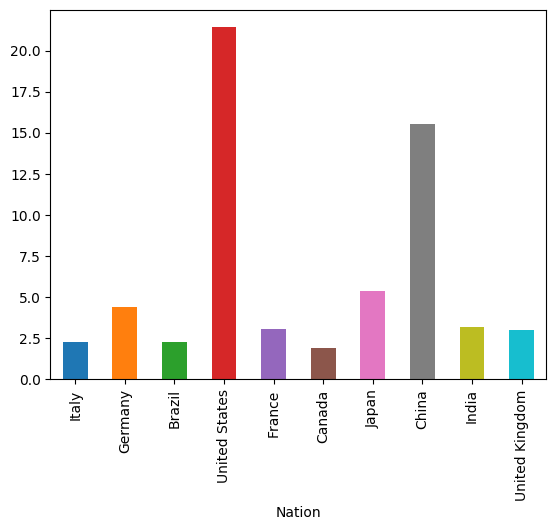
\includegraphics[width=0.7\textwidth]{gdp.png}
\end{figure}

There are a zillion ways to customize these plots, and I'll only mention a
very, very few. A more complete list of options is available by Googling, or
going to \url{https://matplotlib.org/3.1.1/api/\_as\_gen/matplotlib.pyplot.plot.html}

\index{sort\_values@\texttt{.sort\_values()} method (Pandas)}

For instance, to make all the bars the same color, we can pass
``\texttt{color="blue"}''. Sorting the values is something we already know how
to do, with \texttt{.sort\_values()}:

\begin{Verbatim}[fontsize=\small,samepage=true,frame=single,framesep=3mm]
gdp.sort_values(ascending=False).plot(kind='bar')
\end{Verbatim}

\begin{figure}[ht]
\centering
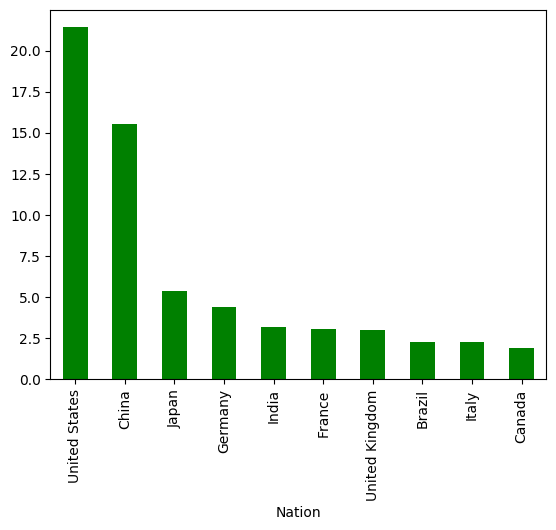
\includegraphics[width=0.7\textwidth]{gdp2.png}
\end{figure}

You see what I mean about ``caring about the labels/keys/index'' for this sort
of plot: if we hadn't labeled the bars, the plot would tell us nothing useful.

I'm sure you've seen lots of bar charts in your life, so this is nothing new.
But consider how much information is embedded in this infographic. Not only can
we tell that the U.S.~and China are the two biggest economies, we can tell that
they are \textit{far and away} the two biggest, with Japan and Germany (the
next two highest) only a fraction.

\subsection{Bar charts of occurrence counts}

\label{categoricalDataBarCharts}

\index{value\_counts@\texttt{.value\_counts()} method (Pandas)}
\index{bar chart}

A very common special case of a bar chart is one where we combine it with the
\texttt{.value\_counts()} method. Let's go back to Taylor vs.~Katy:

\begin{Verbatim}[fontsize=\scriptsize,samepage=true,frame=single,framesep=3mm]
print(faves)
\end{Verbatim}
\vspace{-.3in}

\begin{Verbatim}[fontsize=\scriptsize,samepage=true,frame=leftline,framesep=5mm,framerule=1mm]
0          Katy Perry
1             Rihanna
2       Justin Bieber
3               Drake
4             Rihanna
5        Taylor Swift
6               Adele
7               Adele
8        Taylor Swift
9       Justin Bieber
...
1395       Katy Perry
dtype: object
\end{Verbatim}

\index{plot@\texttt{.plot()} method}

It would be useful to see an infographic on how popular each celebrity is, and
combining \texttt{.value\_counts()} and \texttt{.plot()} makes it a snap:

\begin{Verbatim}[fontsize=\small,samepage=true,frame=single,framesep=3mm]
faves.value_counts().plot(kind='bar',color="orange")
\end{Verbatim}

\begin{figure}[ht]
\centering
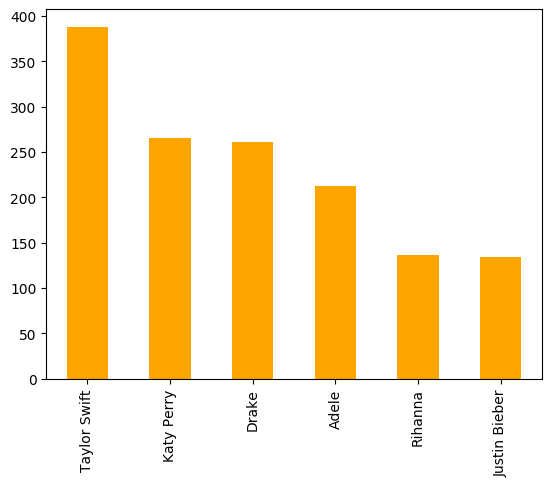
\includegraphics[width=0.6\textwidth]{celebs.png}
\end{figure}

\index{sort\_index@\texttt{.sort\_index()} method (Pandas)}
\index{value\_counts@\texttt{.value\_counts()} method (Pandas)}

The \texttt{.sort\_values()} method wasn't needed here, because our friend
\texttt{.value\_counts()} already returns its answer in decreasing numerical
order. If we wanted the bars in alphabetical order instead, we'd just sort the
\texttt{Series} by index before plotting:

\begin{Verbatim}[fontsize=\small,samepage=true,frame=single,framesep=3mm]
faves.value_counts().sort_index().plot(kind='bar',
    color="purple")
\end{Verbatim}

\begin{figure}[ht]
\centering
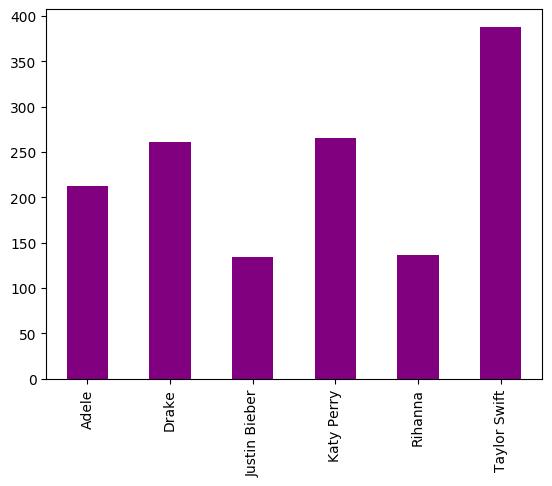
\includegraphics[width=0.6\textwidth]{celebs2.png}
\end{figure}

These long lines with lots of strung-together methods are concise, but can also
be confusing. It's always an option to use temporary variables to store the
intermediate results instead:

\begin{Verbatim}[fontsize=\small,samepage=true,frame=single,framesep=3mm]
counts = faves.value_counts()
alphbetical_counts = counts.sort_index()
alphbetical_counts.plot(kind='bar',color="purple")
\end{Verbatim}

Just a matter of preference.

\section{Numerical data: histograms}

\index{objects (of a study)}

As I mentioned on p.~\pageref{twoWaysToPlotUnivariateData}, sometimes we don't
actually care about the labels in a \texttt{Series}, only the values. This is
when we're trying to size up how \textit{often} values of various magnitudes
appear, irrespective of which specific objects of study those values go with.

\index{histogram}
\index{quantile}
\index{bin (of a histogram)}

My favorite plot this is the \textbf{histogram}. It's super powerful if you
know how to read it, but underused because few people seem to know how. The
idea is that we take a numeric, univariate data set, and divide it up into
\textbf{bins}. Bins are sort of the reverse of quantiles: all bins have the
\textit{same} size range, but a \textit{different} number of data points fall
into each one.

\index{football}
\index{NCAA}
\label{NCAAData}

Suppose we had data on the entire history of a particular NCAA football
conference. A \texttt{Series} called ``\texttt{pts}'' has the number of points
scored by each team in all that conference's games. It looks like this:

\begin{Verbatim}[fontsize=\small,samepage=true,frame=single,framesep=3mm]
print(pts)
\end{Verbatim}
\vspace{-.2in}

\begin{Verbatim}[fontsize=\small,samepage=true,frame=leftline,framesep=5mm,framerule=1mm]
0        7
1       35
2       40
3       17
4       10
...
399     14
dtype: int64
\end{Verbatim}

Some basic summary statistics of interest include:

\begin{Verbatim}[fontsize=\small,samepage=true,frame=single,framesep=3mm]
print("min: {}".format(pts.quantile(0)))
print(".25-quantile: {}".format(pts.quantile(.25)))
print(".5-quantile: {}".format(pts.quantile(.5)))
print(".75-quantile: {}".format(pts.quantile(.75)))
print("max: {}".format(pts.quantile(1)))
print("mean: {}".format(pts.mean()))
\end{Verbatim}
\vspace{-.2in}

\label{ncaaQuantiles}
\begin{Verbatim}[fontsize=\small,samepage=true,frame=leftline,framesep=5mm,framerule=1mm]
min: 0.0
.25-quantile: 17.0
.5-quantile: 25.0
.75-quantile: 32.0
max: 55.0
mean: 23.755
\end{Verbatim}

Looks like a typical score is in the 20's, with the conference record being a
whopping 55 points in one game. The IQR is $32-17$, or 15 points.

We can plot a histogram of this \texttt{Series} with this code:

\begin{Verbatim}[fontsize=\small,samepage=true,frame=single,framesep=3mm]
pts.plot(kind='hist')
\end{Verbatim}

The result is in Figure~\ref{fig:ncaa1}. Stare hard at it. Python has divided
up the points into ranges: 0 through 6 points, 7 through 12 points, 13 through
21, \textit{etc.} Each of these ranges is a bin. The height of each blue bar on
the plot is simply the number of games in which a team scored in that range.

\begin{figure}[ht]
\centering
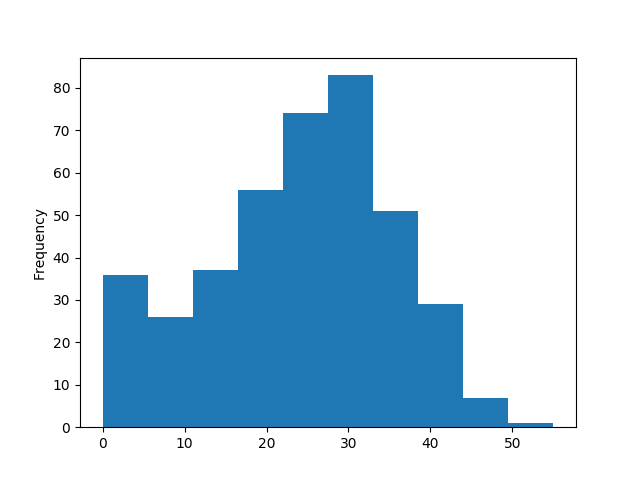
\includegraphics[width=0.9\textwidth]{ncaa1.png}
\caption{A histogram of the historical points-per-game for teams in a certain
NCAA football conference.}
\label{fig:ncaa1}
\end{figure}

\index{bell-curvy@``bell-curvy''}
Now what do we learn from this? Lots, if we know how to read it. For one thing,
it looks like the vast majority of games have teams scoring between 12 and 38
points. A few teams have managed to eke out 40 or more, and there have been a
modest number of single-digit scores or shutouts. Moreover, it appears that
scores between 24 and 38 are considerably more common than those between 12 and
24. Finally, this data shows some evidence of being ``bell-curvy'' in the sense
that values in the middle of the range are more common than values at either
end, and it is (very roughly) symmetrical on both sides of the median.

This is even more precise information than the quantiles gave us. We get an
entire birds-eye view of the data set. Whenever I'm looking at a numerical,
univariate data set, pretty much the first thing I do is throw a histogram up
on the screen and spend at least a couple minutes staring at it. It's almost
the best diagnostic tool available.

\subsection{Bin size}

\index{bin (of a histogram)}
\index{plot@\texttt{.plot()} method}

Now one idiosyncrasy with histograms is that a lot depends on the bin size and
placement. Python made its best guess at a decent bin size here by choosing
ranges of 6 points each. But we can control this by passing a second parameter
to the \texttt{.plot()} function, called ``\texttt{bins}'':

\begin{Verbatim}[fontsize=\small,samepage=true,frame=single,framesep=3mm]
pts.plot(kind='hist', bins=30)
\end{Verbatim}

Here we specifically asked for \textit{thirty} bins in total, and we get the
result in Figure~\ref{fig:ncaa2}. Now each bin is only two points wide, and as
you can see there's a lot more detail in the plot.

\begin{figure}[ht]
\centering
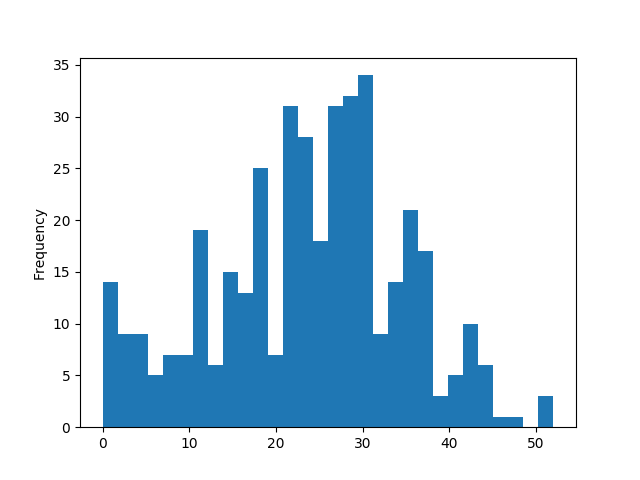
\includegraphics[width=0.9\textwidth]{ncaa2.png}
\caption{The same data set as in Figure~\ref{fig:ncaa1}, but with more (and
smaller) bins.}
\label{fig:ncaa2}
\end{figure}

Whether that amount of detail is a good thing or not takes some practice to
decide. Make your bins too large and you don't get much precision in your
histogram. Make them too small and the trees can overwhelm the forest. In this
case, I'd say that Figure~\ref{fig:ncaa2} is good in that it tells us something
not apparent from Figure~\ref{fig:ncaa1}: there are quite a few shutouts
(zero-point performances), not merely games with six-points-or-less. Whether
the trough between 22 and 24 points is meaningful is another matter, and my
guess is that part is obscuring the more general features apparent in the first
plot.

\index{sweet spot@``sweet spot''}

The rule is: whenever you create a histogram, \textit{take a few minutes to
experiment with different bin sizes.} Often you'll find a ``sweet spot'' where
the amount of detail is just right, and you'll get great insight into the data.
But you do have to work at it a little bit.

\subsection{Non-bell-curvy data}

\index{YouTube}
\index{num\_plays@\texttt{num\_plays}}

Let's return again to the YouTube example. We had some surprises when we looked
at the quantiles and saw that the 1-quantile (max) was astronomically higher
than the .9-quantile was. Let's see what happens when we plot a histogram
(show in Figure~\ref{fig:youtube1}):

\begin{Verbatim}[fontsize=\scriptsize,samepage=true,frame=single,framesep=3mm]
num_plays.plot(kind='hist', color="red")
\end{Verbatim}

\begin{figure}[ht]
\centering
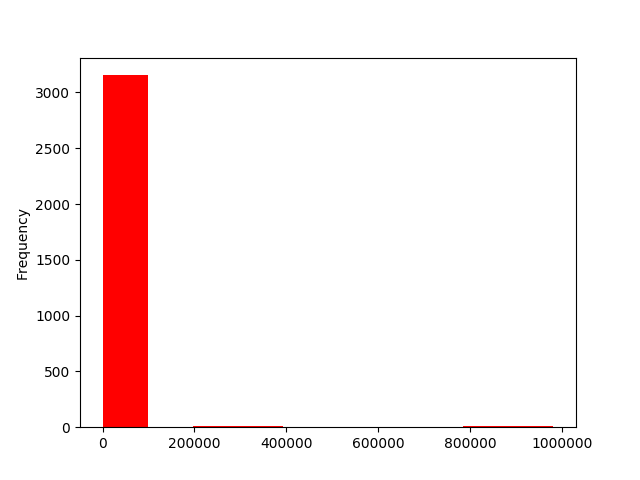
\includegraphics[width=1\textwidth]{youtube1.png}
\caption{A first attempt at plotting the YouTube \texttt{num\_plays} data set.}
\label{fig:youtube1}
\end{figure}

Huh?? Wait, where are all the bars of varying heights? We seem to have got only
a single one.

But they're there! They're just so small you can't see them. If you stare at
the x-axis -- and your eyesight is good -- you might see tiny signs of life at
higher values. But the overall picture is clear: the vast, vast majority of
videos in this set have between 0 and 100,000 plays.

\index{bin (of a histogram)}

Let's see if we can get more detail by increasing the number of bins (say,
to 1000):

\begin{Verbatim}[fontsize=\scriptsize,samepage=true,frame=single,framesep=3mm]
num_plays.plot(kind='hist', bins=1000, color="red")
\end{Verbatim}

We now get the left-hand side of Figure~\ref{fig:youtube23}. It didn't really
help much. Turns out the masses aren't merely crammed below a hundred thousand
plays; they're crammed below \textit{one} thousand. We need another approach if
we're going to see any detail on the low-play videos.

\begin{figure}[ht]
\centering
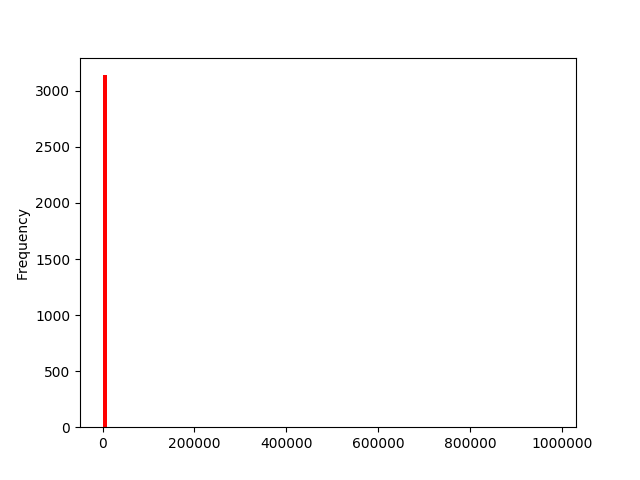
\includegraphics[width=.48\textwidth]{youtube2.png}
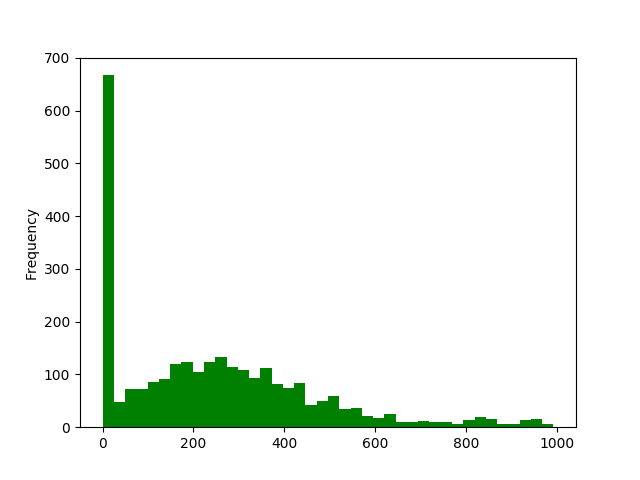
\includegraphics[width=.48\textwidth]{youtube3.png}
\caption{Further attempts at plotting the YouTube \texttt{num\_plays} data set.
On the left side, we decreased the bin size to no avail. On the right side, we
gave up on plotting the popular videos and concentrated only on the unpopular
ones, which does illuminate the lower end somewhat. (Don't miss the x-axis
ranges!)}
\label{fig:youtube23}
\end{figure}


\index{distribution}
\index{query}
\index{filter}

The only way to really see the distribution on the low end is to \textit{only}
plot the low end. Let's use a query (recall section~\ref{seriesQueries} from
p.~\pageref{seriesQueries}) to filter out \textit{only} the videos with 1000
plays or fewer, and then plot a histogram of that:

\begin{Verbatim}[fontsize=\footnotesize,samepage=true,frame=single,framesep=3mm]
unpopular_video_plays = num_plays[num_plays <= 1000]
unpopular_video_plays.plot(kind='hist', color="green")
\end{Verbatim}

This gives the right-hand side of Figure~\ref{fig:youtube23}. Now we can at
least see what's going on. Looks like our \texttt{Series} has a crap-ton of
videos that have never been viewed at all (recall our .1-quantile epiphany for
this data set on p.\pageref{pointOneQuantileEpiphany}) plus a chunk that are in
the 500-views-or-fewer range.

\index{bell-curvy@``bell-curvy''}
\index{mean}
\index{standard deviation}
\index{Broadway shows}

The takeaway here is that not all data sets (by a long shot!) are bell-curvy.
Statistics courses often present nice, symmetric data sets on physical
phenomena like bridge lengths or actor heights or free throw percentages, which
have nice bell curves and are nicely summarized by means and standard
deviations. But for many social phenomena (like salaries, numbers of
likes/followers/plays, lengths of Broadway show runs, \textit{etc.})~the data
looks more like this YouTube example. A few extremely large values dominate
everything else by their sheer magnitude, which makes it more difficult to wrap
your head around.

It also makes it more challenging to answer the question, ``what's the
\textit{typical} value for this variable?'' It ain't the mean, that's for sure.
If you asked me for the ``typical'' number of plays of one of these YouTube
videos, I'd probably say ``zero'' since that's an extremely common value.
Another reasonable answer would be ``somewhere in the low hundreds,'' since
there are quite a few videos in that range, as illustrated by the
right-hand-side of Figure~\ref{fig:youtube23}. But you'd be hard-pressed to try
and sum up the entire data set with a single typical value. There just isn't
one for stuff like this.

\section{Numerical data: box plots}

\index{bivariate}
\index{box plot}
\index{plot@\texttt{.plot()} method}

Let's talk about one more type of plot in this chapter, even though it's really
most useful when dealing with bivariate data, as we'll address in
chapter~\ref{ch:edaBivariate2}. It's called the \textbf{box plot} (also known
as a ``\textbf{box-and-whisker'' plot}). We can create one by passing
``\texttt{kind="box"}'' to the \texttt{.plot()} method (here for the NCAA
football data):

\begin{Verbatim}[fontsize=\small,samepage=true,frame=single,framesep=3mm]
pts.plot(kind="box")
\end{Verbatim}

\label{interpretingBoxPlots}

The result is shown in Figure~\ref{fig:ncaaBox}, along with some annotations in
red so you can figure out what's going on.

\begin{figure}[ht]
\centering
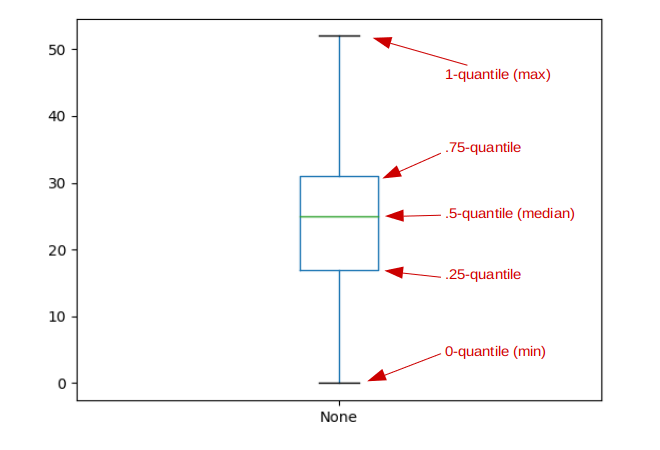
\includegraphics[width=1\textwidth]{ncaaboxAnnotated.png}
\caption{A box plot of the NCAA points data.}
\label{fig:ncaaBox}
\end{figure}

For now, don't worry about the mysterious word ``\texttt{None}'' at the bottom.
(This indicates which ``group'' the box represents, and will feature
prominently in our bivariate data chapter.) For a univariate data set like this
one, the x-axis has no meaning. The y-axis, on the other hand, is easy to
understand: it's the number of points per football game.

\index{quantile}

Now the thing to realize about box plots is that they're essentially just a
graphical way of showing quartiles; or, put another way, a graphical way of
showing these five quantiles:

\begin{compactitem}
\item The 0-quantile (the minimum value) is the y-value of the bottom ``whisker.''
\item The .25-quantile is the y-value of the bottom of the ``box.''
\item The .5-quantile (the median) is the y-value of the horizontal line within
the box.
\item The .75-quantile is the y-value of the top of the ``box.''
\item The 1-quantile (the maximum value) is the y-value of the top ``whisker.''
\end{compactitem}

\index{IQR (interquartile range)}
Using your quantile knowledge from section~\ref{quantiles}, you'll realize the
following fact: \textit{the box alone contains exactly half the data points.}
This is a key insight. While the whiskers show the entire range of the data,
the box shows the middle 50\% of it. (And the height of the box is precisely
the IQR.) This makes it very easy to grasp where the bulk of the data lies, and
it reinforces the lesson we learned from the histogram on this data set
(Figure~\ref{fig:ncaa1} on page \pageref{fig:ncaa1}): a big chunk of the time,
teams score in the 20's.

You might object to showing an entire plot for this, since I've just revealed
that it's merely a fancy way to show five numbers. And you're right, in a way.
However, when we show multiple \textit{groups} of data side-by-side, each with
their own box, it becomes a particularly powerful tool. Stay tuned for that.

\subsection{Outliers}

What happens if we show our head-scratching YouTube data set as a box plot? You
get the monstrosity in Figure~\ref{fig:youtubebox}.

\begin{figure}[ht]
\centering
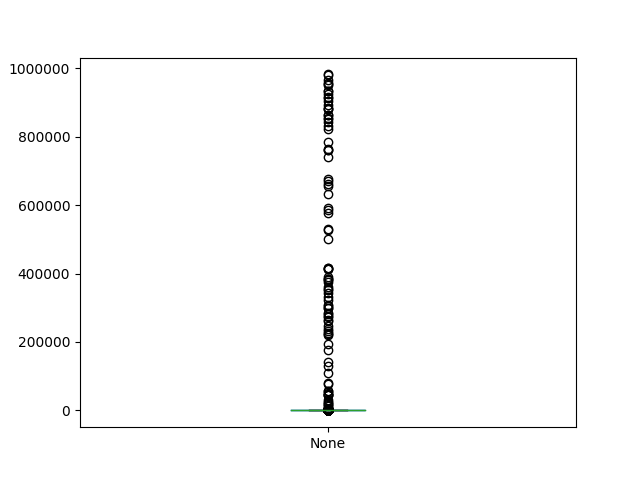
\includegraphics[width=0.8\textwidth]{youtubebox.png}
\caption{A box plot of a non-bell-curvy data set.}
\label{fig:youtubebox}
\end{figure}

\index{outlier}
\index{fish bubbles}

Geez Louise, does that look wacky. The little circles (which to me always
looked like bubbles from fish breath) represent \textbf{outliers}, an important
concept in data science. An outlier is basically any data point that's so far
out of the normal range that it seems strange. Python is essentially flagging
it for us, so we can judge for ourselves whether it was a data entry error or
just a strange data point. In this case, these aren't errors -- there's just a
handful of videos that have been played a ton of times. And this makes the
whole box plot look weird.

\index{gravity}
\index{black hole}
\index{smoosh}

Notice from Figure~\ref{fig:youtubebox} that \textit{the entire box and both
whiskers} have gotten smooshed at the bottom of the figure, as if crushed by
the gravity of a black hole. You'll see that the top whisker doesn't
\textit{really} mean ``maximum,'' since it's way down there in thousand-land
despite the fact that we have videos with almost a million views. The top
whisker truly means ``the maximum \textit{reasonable-looking} data point in the
\texttt{Series},'' where ``reasonable-looking'' is something Pandas is trying
to make an educated guess about. There are ways to tweak what counts as an
outlier, but my purpose here is just to get you to realize that when you have a
highly skewed data set (like YouTube), prepare to see lots of things that are
considered ``outliers,'' and prepare to comb through all the mess on your box
plots to try and discern the true meaning it's trying to convey.


\chapter[Tables in Python (1 of 3)]{\huge\selectfont{Tables in Python (1 of
3)}}

\label{dataframes}

\index{table}
\index{DataFrame@\texttt{DataFrame} (Pandas)}

The third of our three aggregate data types from waaaay back in
Chapter~\ref{ch:aggregateData} was the \textbf{table}. Don't worry: we haven't
forgotten about him. In this chapter, we'll implement him by means of the
Pandas \texttt{DataFrame}, the most important data type in this entire book.

\section{Reading a \texttt{DataFrame} from a \texttt{.csv} file}

\index{CSV@CSV (comma-separated values format)}

Unlike NumPy arrays and Pandas \texttt{Series}es, which we learned several
different ways to create, we're only going to learn one way to create a
\texttt{DataFrame}. That's because \texttt{DataFrame}s are normally big enough
that it's just too tedious to ever type them in manually. Instead, we'll read
them from an external source; namely, a \texttt{.csv} file.

\index{read\_csv@\texttt{read\_csv()} function (Pandas)}
\index{davieses@\texttt{davieses}}

We'll actually use the same \texttt{read\_csv()} function that we used in
section~\ref{read_csv} (p.~\pageref{read_csv}), although oddly, this time we
won't need to specify as many arguments. Let's say we have a
``\texttt{davieses.csv}'' file with these contents:

\index{file!\texttt{.csv}}

\begin{Verbatim}[fontsize=\small,samepage=true,frame=lines,framesep=3mm]
person,age,gender,height,instrument
Dad,50,M,73,piano
Mom,49,F,66,flute
Lizzy,19,F,63,guitar
TJ,18,M,71,trombone
Johnny,15,M,69,euphonium
\end{Verbatim}

We can read it into a \texttt{DataFrame} with this code:

\begin{Verbatim}[fontsize=\small,samepage=true,frame=single,framesep=3mm]
my_first_data_frame = pd.read_csv("davieses.csv").set_index('person')
print(my_first_data_frame)
\end{Verbatim}
\vspace{-.2in}

\begin{Verbatim}[fontsize=\small,samepage=true,frame=leftline,framesep=5mm,framerule=1mm]
        age gender  height instrument
person                               
Dad      50      M      73      piano
Mom      49      F      66      flute
Lizzy    19      F      63     guitar
TJ       18      M      71   trombone
Johnny   15      M      69  euphonium
\end{Verbatim}

\index{header row (of a \texttt{.csv} file)}
\index{row (of a table)}

A couple things. First, you may have noticed that the \texttt{davieses.csv}
file had a ``header'' row. This means that the first line of the file is not
like the others: instead of containing information on a specific family member,
it contains the \textit{kind} of information for \textit{every} family member.
It looked like this:

\vspace{-.1in}
\begin{center}
\texttt{person,age,gender,height,instrument}
\end{center}
\vspace{-.1in}

\index{column (of a table)}
\index{metadata}

and you'll notice that these words (except for the first one; more on that in a
moment) became the \textit{column names} when we imported the data. This sort
of information, by the way, is called ``\textbf{metadata},'' a geeky-sounding
word that basically means ``data about data.'' If ``Lizzy plays the guitar'' is
a piece of data, then ``family members play instruments'' is a piece of
\textit{meta}data.

\index{read\_csv@\texttt{read\_csv()} function (Pandas)}
\index{set\_index@\texttt{set\_index()} method (Pandas)}

Second, don't miss the ending I tacked on to the \texttt{read\_csv()} line,
where I called the \texttt{.set\_index()} method on the \texttt{DataFrame}.
This tells Pandas that one of the columns in the \texttt{DataFrame} should be
designated as the \textbf{index} (or the \textbf{keys}).

\index{uniqueness!of the values in a \texttt{DataFrame} index}

Back on p.~\pageref{tablesHaveNoKey} I asserted that unlike associative arrays,
tables didn't have keys. And that's true of the general ``table'' concept. But
Pandas designed their \texttt{DataFrame}s to behave in the same way as their
\texttt{Series}es: one uniquely-valued column will be used to identify each
row.

\index{Foreman, George}
\index{George}

This choice is usually easy; if you glance back to Figure~\ref{fig:table}
(p.~\pageref{fig:table}), we'd probably want to choose the \textsf{screenname}
as the index (although a case could be made for the \textsf{real name} column
instead). For the table in Figure~\ref{fig:aggregateMemory}
(p.~\pageref{fig:aggregateMemory}), it would be the \textsf{item} column. In
the \texttt{DataFrame} we just created above, obviously \texttt{person} is the
correct choice -- it's the only one sure to be unique.\footnote{With apologies
to boxing legend George Foreman, who named all four of his sons ``George.''}

Anyway, designating a column as the index in this way sort of removes it from
the other, ``ordinary'' columns. In the output, above, you may notice that the
word ``\texttt{person}'' is printed somewhat lower than the other column names
are. It turns out that if we want to talk about the index column specifically,
we'll need to use a slightly different technique than we do for the other
columns. More on that next chapter.

\section{Missing values}

Let's change the example to a different family, and a slightly bigger
\texttt{DataFrame}. The ``\texttt{simpsons.csv}'' file is reproduced below. Do
you notice anything odd about it?

\index{simpsons@The Simpsons}
\index{Santa's Little Helper}
\index{file!\texttt{.csv}}

\begin{Verbatim}[fontsize=\small,samepage=true,frame=lines,framesep=3mm]
name,species,age,gender,fave,IQ,hair,salary
Homer,human,36,M,beer,74,,52000
Marge,human,34,F,helping others,120,stacked tall,
Bart,human,10,M,skateboard,90,buzz,
Lisa,human,8,F,saxophone,200,curly,
Maggie,human,1,F,pacifier,100,curly,
SLH,dog,4,M,,,shaggy,
\end{Verbatim}

\index{double comma@``double comma''}

What I mean is the positioning of some of the commas. The sharp-eyed reader
will see a ``double comma'' in Homer's row. Even a dull-eyed reader will notice
several commas in a row in SLH's\footnote{The Simpson's dog was named ``Santa's
Little Helper.''} row. And nearly \textit{every} row (the exception being
Homer's) \textit{ends} with a comma, which just looks messed up.

\index{missing value}

This weird punctuation implies the existence of \textbf{missing values}, which
means just what it sounds like: there's simply no data for certain columns of 
certain rows. Homer doesn't have a ``\texttt{hair}'' value, no one \textit{but}
Homer has a ``\texttt{salary}'' value, and SLH is missing all kinds of stuff.

When we read this into a Pandas \texttt{DataFrame} a la:

\begin{Verbatim}[fontsize=\small,samepage=true,frame=single,framesep=3mm]
simpsons = pd.read_csv("simpsons.csv").set_index('name')
\end{Verbatim}

the result looks like this:

\begin{Verbatim}[fontsize=\small,samepage=true,frame=leftline,framesep=5mm,framerule=1mm]
       species  age gender            fave     IQ          hair   salary
name                                                                    
Homer    human   36      M            beer   74.0           NaN  52000.0
Marge    human   34      F  helping others  120.0  stacked tall      NaN
Bart     human   10      M      skateboard   90.0          buzz      NaN
Lisa     human    8      F       saxophone  200.0         curly      NaN
Maggie   human    1      F        pacifier  100.0         curly      NaN
SLH        dog    4      M             NaN    NaN        shaggy      NaN
\end{Verbatim}

\index{nan@\texttt{NaN} (``not a number'')}

The missing values come up as \texttt{NaN}'s, the same value you may remember
from p.~\pageref{NaN}. The monker ``not a number'' makes sense for the
\texttt{salary} case, although I think it's a bit weird for Homer's
\texttt{hair} (not a number? is hair \textit{supposed} to be a number?...)
At any rate, we can expect that this will be the case for many real-world data
sets.

\index{objects (of a study)}

``Missing'' can mean quite a few subtly different things, actually. Maybe it
means that the value for that object of study was collected, but lost. Maybe it
means it was never collected at all. Maybe it means that variable doesn't
really make \textit{sense} for that object, as in the case of a dog's IQ.
Ultimately, if we want to use the other values in that row, we'll have to come
to terms with what the missing values \textit{mean}. For now, let's just learn
a couple of coarse ways of dealing with them.

\index{dropna@\texttt{.dropna()} method (Pandas)}

One (sometimes) handy method is \texttt{.dropna()}. If you call it, it will
return a modified copy of the \texttt{DataFrame} in which any row with an
\texttt{NaN} is removed. This turns out to be overkill in the Simpson's case,
though:

\begin{Verbatim}[fontsize=\small,samepage=true,frame=single,framesep=3mm]
print(simpsons.dropna())
\end{Verbatim}
\vspace{-.2in}

\begin{Verbatim}[fontsize=\small,samepage=true,frame=leftline,framesep=5mm,framerule=1mm]
Empty DataFrame
Columns: [species, age, gender, fave, IQ, hair, salary]
Index: []
\end{Verbatim}

In other words, nothing's left. (Every row had at least one \texttt{NaN} in
it, so nothing survived.)

We could pass an optional argument to \texttt{.dropna()} called
``\texttt{how}'', and set it equal to \texttt{"all"}: in this case only rows
with \textit{all} \texttt{NaN} values are removed. Sometimes that's
``underkill,'' as in our Simpson's example: after all, none of the rows are
\textit{entirely} \texttt{NaN}'s, so calling \texttt{.dropna(how="all")}
would leave everything intact.

\index{fillna@\texttt{.fillna()} method (Pandas)}
\index{default value}

Another option is the \texttt{.fillna()} method, which takes a ``default
value'' argument: any \texttt{NaN} value is replaced with the default in the
modified copy returned. Let's try it with the string \texttt{"none"} as the
default value:

\begin{Verbatim}[fontsize=\small,samepage=true,frame=single,framesep=3mm]
print(simpsons.fillna("none"))
\end{Verbatim}
\vspace{-.2in}

\begin{Verbatim}[fontsize=\small,samepage=true,frame=leftline,framesep=5mm,framerule=1mm]
       species  age gender            fave    IQ          hair salary
name                                                                 
Homer    human   36      M            beer    74          none  52000
Marge    human   34      F  helping others   120  stacked tall   none
Bart     human   10      M      skateboard    90          buzz   none
Lisa     human    8      F       saxophone   200         curly   none
Maggie   human    1      F        pacifier   100         curly   none
SLH        dog    4      M            none  none        shaggy   none
\end{Verbatim}

This is possibly useful, but in this case it's not a perfect fit because
different columns call for different defaults. The \texttt{fave} and
\texttt{hair} columns could well have ``\texttt{none}'' (indicating no
favorite thing, and no hair, respectively) but we might want the default
\texttt{salary} to be 0. The way to accomplish that is to change the individual
columns of the \texttt{DataFrame}. Here goes:

\begin{Verbatim}[fontsize=\small,samepage=true,frame=single,framesep=3mm]
simpsons['salary'] = simpsons['salary'].fillna(0)
simpsons['IQ'] = simpsons['IQ'].fillna(100)
simpsons['hair'] = simpsons['hair'].fillna("none")
print(simpsons)
\end{Verbatim}
\vspace{-.2in}

\begin{Verbatim}[fontsize=\small,samepage=true,frame=leftline,framesep=5mm,framerule=1mm]
       species  age gender            fave     IQ          hair   salary
name                                                                    
Homer    human   36      M            beer   74.0          none  52000.0
Marge    human   34      F  helping others  120.0  stacked tall      0.0
Bart     human   10      M      skateboard   90.0          buzz      0.0
Lisa     human    8      F       saxophone  200.0         curly      0.0
Maggie   human    1      F        pacifier  100.0         curly      0.0
SLH        dog    4      M             NaN  100.0        shaggy      0.0
\end{Verbatim}

Here we've assumed that the default IQ, for someone who hasn't taken the test,
is 100 (the average). I left the \texttt{NaN} in \texttt{fave} as is, since
that seemed appropriate.

\begin{samepage}
By the way, that code is actually more than it may appear at first. When we
execute a line like:

\vspace{-.1in}
\begin{center}
\texttt{simpsons[\textquotesingle salary\textquotesingle] =
simpsons[\textquotesingle salary\textquotesingle].fillna(0)}
\end{center}
\vspace{-.1in}
\end{samepage}

we're really saying ``please \textit{replace} the \texttt{salary} column of the
\texttt{simpsons} \texttt{DataFrame} with a new column. That new column should
be -- wait for it -- the existing \texttt{salary} column but with zeros
replacing the \texttt{NaN}'s.''

We'll see many more cases of changing \texttt{DataFrame} columns wholesale in
the following chapters.

\section{Removing rows/columns}

Finally, there are times when after reading a \texttt{.csv} file into a
\texttt{DataFrame}, you want to manually delete certain rows and/or columns
that are not going to be of interest.


\begin{samepage}

\index{drop@\texttt{.drop()} method (Pandas)}
\index{Santa's Little Helper}
The easiest syntax for deleting a row (say, Santa's Little Helper) is:

\begin{Verbatim}[fontsize=\small,samepage=true,frame=single,framesep=3mm]
simpsons = simpsons.drop('SLH')
\end{Verbatim}
\end{samepage}

The \texttt{.drop()} method takes the index of the undesired row as an
argument, Like most of the methods we've seen so far, it returns a modified
copy of the \texttt{DataFrame} it's called on, so you have to reassign this to
the original variable (or use the \texttt{inplace=True} argument).

\index{boxies (square brackets)}
\index{[]@\texttt{[]} (boxies)}

\begin{samepage}
You can even delete multiple rows at the same time by enclosing the undesired
indices in boxies:

\begin{Verbatim}[fontsize=\small,samepage=true,frame=single,framesep=3mm]
simpsons = simpsons.drop(['Homer','Marge','SLH'])
\end{Verbatim}
\end{samepage}

\begin{samepage}

\index{del operator@\texttt{del} operator (Pandas)}
Deleting a column is even more common, since many tables ``in the wild'' have
many, many columns, only a few of which you may care about in your analysis.
You can whack one entirely with the \texttt{del} operator, just like we did for
\texttt{Series}es (p.~\pageref{delOp}):

\begin{Verbatim}[fontsize=\small,samepage=true,frame=single,framesep=3mm]
del simpsons['IQ']
\end{Verbatim}
\end{samepage}


\chapter[Tables in Python (2 of 3)]{\huge\selectfont{Tables in Python (2 of
3)}}

\label{tablesInPython2}
\index{row (of a \texttt{DataFrame})}
\index{row (of a table)}
\index{column (of a table)}

It's easy to get tripped up on Pandas' syntax for accessing the individual bits
of \texttt{DataFrame}s. First, let's talk about rows and columns, and then
we'll talk about the atomic elements (``cells'') themselves.

\section{Accessing individual rows and columns}

\label{accessIndividualRowsColsOfDataFrame}

Suppose you have a \texttt{DataFrame} called \texttt{df}. Here's how you can
extract particular rows and columns:

\begin{compactitem}
\item \texttt{df.loc[}\textsl{i}\texttt{]} -- access the \textbf{row} with
\textbf{index} \textsl{i}
\item \texttt{df.iloc[}\textsl{n}\texttt{]} -- access \textbf{row} number
\textsl{n}
\item \texttt{df[}\textsl{c}\texttt{]} -- access \textbf{column} \textsl{c}
\end{compactitem}

\index{iloc@\texttt{.iloc} syntax (Pandas)}
\index{loc@\texttt{.loc} syntax (Pandas)}

The second of these is reminiscent of the \texttt{.iloc} syntax we learned for
\texttt{Series}es on p.~\pageref{iloc}. With it, we specify the \textit{number}
we want, rather than the index/key/label. That's not super common to do, but it
happens. More common is the first form: we specify the row we want by its
index.

The last one is tricky, because everyone (including me, several times a week,
it seems) assumes that just typing (say) ``\texttt{df['Bart']}'' would give you
\texttt{Bart}'s row. This is probably how it \textit{ought} to work, since
\texttt{Series}es worked that way. Alas, no: if you specify neither
\texttt{.loc} nor \texttt{.iloc}, you're asking for a \textit{column}, not a
row.

% WARNING: "bottom of" might not be correct if we change ch.16 text.

Yet another odd thing is how a single row is presented on the screen. Let's go
back to the \texttt{simpsons} data set (bottom of p.~\pageref{finalSimpsons}),
and access the \texttt{Bart} row the proper way (with \texttt{.loc}):

\begin{Verbatim}[fontsize=\small,samepage=true,frame=single,framesep=3mm]
print(simpsons.loc['Bart'])
\end{Verbatim}
\vspace{-.2in}

\begin{Verbatim}[fontsize=\small,samepage=true,frame=leftline,framesep=5mm,framerule=1mm]
species         human
age                10
gender              M
fave       skateboard
IQ                 90
hair             buzz
salary              0
Name: Bart, dtype: object
\end{Verbatim}

This bugs the heck out of me. Bart, like all other Simpsons, was a \textit{row}
in the original \texttt{DataFrame}, but here, it presents Bart's information
vertically instead of horizontally. I find it visually jarring. The reason
Pandas does it this way is that \textit{each row of a \texttt{DataFrame} is a
\texttt{Series}}, and the way Pandas displays \texttt{Series}es is vertically.
We'll deal somehow.

\index{double boxies@``double boxies''}

Btw, for any of the three options, you can provide a \textit{list} with
multiple things you want, instead of just one thing. You do so by using
\textit{double} boxies:

\begin{compactitem}
\item \texttt{df.loc[[}\textsl{i1,i2,i3,\dots}\texttt{]]} -- access the
row\textbf{s} with indices \textsl{i1, i2, i3,} \textit{etc.}
\item \texttt{df.iloc[[}\textsl{n1,n2,n3,\dots}\texttt{]]} -- access the row\textbf{s}
numbered \textsl{n1, n2, n3,} \textit{etc.}
\item \texttt{df[[}\textsl{c1,c2,c3,\dots}\texttt{]]} -- access the
column\textbf{s} names \textsl{c1, c2, c3,} \textit{etc.}
\end{compactitem}

\subsection{Examples}

To test your understanding of all of the above, confirm that you understand the
following examples:

\begin{Verbatim}[fontsize=\scriptsize,samepage=true,frame=single,framesep=3mm]
print(simpsons.iloc[3])
\end{Verbatim}
\vspace{-.2in}

\begin{Verbatim}[fontsize=\scriptsize,samepage=true,frame=leftline,framesep=5mm,framerule=1mm]
species        human
age                8
gender             F
fave       saxophone
IQ               200
hair           curly
salary             0
Name: Lisa, dtype: object
\end{Verbatim}

\medskip

\begin{Verbatim}[fontsize=\scriptsize,samepage=true,frame=single,framesep=3mm]
print(simpsons['age'])
\end{Verbatim}
\vspace{-.2in}

\begin{Verbatim}[fontsize=\scriptsize,samepage=true,frame=leftline,framesep=5mm,framerule=1mm]
name
Homer     36
Marge     34
Bart      10
Lisa       8
Maggie     1
SLH        4
Name: age, dtype: int64
\end{Verbatim}

\medskip
\begin{Verbatim}[fontsize=\scriptsize,samepage=true,frame=single,framesep=3mm]
print(simpsons.loc[['Lisa','Maggie','Bart']])
\end{Verbatim}
\vspace{-.2in}

\begin{Verbatim}[fontsize=\scriptsize,samepage=true,frame=leftline,framesep=5mm,framerule=1mm]
       species  age gender        fave     IQ   hair  salary
name                                                        
Lisa     human    8      F   saxophone  200.0  curly     0.0
Maggie   human    1      F    pacifier  100.0  curly     0.0
Bart     human   10      M  skateboard   90.0   buzz     0.0
\end{Verbatim}

\medskip
\begin{Verbatim}[fontsize=\scriptsize,samepage=true,frame=single,framesep=3mm]
print(simpsons.iloc[[1,3,4]])
\end{Verbatim}
\vspace{-.2in}

\begin{Verbatim}[fontsize=\scriptsize,samepage=true,frame=leftline,framesep=5mm,framerule=1mm]
       species  age gender            fave     IQ          hair  salary
name                                                                   
Marge    human   34      F  helping others  120.0  stacked tall     0.0
Lisa     human    8      F       saxophone  200.0         curly     0.0
Maggie   human    1      F        pacifier  100.0         curly     0.0
\end{Verbatim}

\medskip
\begin{Verbatim}[fontsize=\scriptsize,samepage=true,frame=single,framesep=3mm]
print(simpsons[['age','fave','IQ']])
\end{Verbatim}
\vspace{-.2in}

\begin{Verbatim}[fontsize=\scriptsize,samepage=true,frame=leftline,framesep=5mm,framerule=1mm]
        age            fave     IQ
name                              
Homer    36            beer   74.0
Marge    34  helping others  120.0
Bart     10      skateboard   90.0
Lisa      8       saxophone  200.0
Maggie    1        pacifier  100.0
SLH       4             NaN   30.0
\end{Verbatim}

Incidentally, you'll notice how the \texttt{name} values are treated
differently from all the other columns, since \texttt{name} is the
\texttt{DataFrame}'s index. For one thing, \texttt{name} \textit{always}
appears, even though it's not included among the columns we asked for. For
another, it's listed at the bottom of the single-row \texttt{Series} listings
rather than up with the other values in that row.

\section{Accessing individual elements}

\label{accessIndividualElementsOfDataFrame}

I mentioned above the eternal truth that \textit{each row of a
\texttt{DataFrame} is a \texttt{Series}}. Once you grasp this, you'll realize
that you can access an individual ``cell'' of a \texttt{DataFrame} simply by
getting the row you want, and then getting the specific value from that. A
two-step process for doing this would be:

\begin{Verbatim}[fontsize=\small,samepage=true,frame=single,framesep=3mm]
lisas_row = simpsons.loc['Lisa']
lisas_iq = lisas_row['IQ']
print(lisas_iq)
\end{Verbatim}
\vspace{-.2in}

\begin{Verbatim}[fontsize=\small,samepage=true,frame=leftline,framesep=5mm,framerule=1mm]
200.0
\end{Verbatim}

But a shorter, one-stepper just combines these two operations on the same line:

\begin{Verbatim}[fontsize=\small,samepage=true,frame=single,framesep=3mm]
lisas_iq = simpsons.loc['Lisa']['IQ']
print(lisas_iq)
\end{Verbatim}
\vspace{-.2in}

\begin{Verbatim}[fontsize=\small,samepage=true,frame=leftline,framesep=5mm,framerule=1mm]
200.0
\end{Verbatim}

\section{Accessing a \texttt{DataFrame}'s metadata}

\index{metadata}
\index{index@\texttt{.index} (little \texttt{i}) syntax}

We can get some meta-information about a \texttt{DataFrame} without even
looking at individual rows. If we want to know what the index values themselves
are, we use \texttt{.index}:

\begin{Verbatim}[fontsize=\small,samepage=true,frame=single,framesep=3mm]
print(simpsons.index)
\end{Verbatim}
\vspace{-.2in}

\begin{Verbatim}[fontsize=\small,samepage=true,frame=leftline,framesep=5mm,framerule=1mm]
Index(['Homer', 'Marge', 'Bart', 'Lisa', 'Maggie', 'SLH'],
    dtype='object', name='name')
\end{Verbatim}

That weird-looking output tells us several things. First, the index of this
\texttt{DataFrame} consists of \texttt{string}s (remember from
p.~\pageref{dtypeRules} that's what ``\texttt{dtype=\textquotesingle
object\textquotesingle}'' means). Second,
the \textit{name} of the index column is, ironically, ``\texttt{name}''. (It
could be named anything at all, of course.) Third, the actual index values are
\texttt{Homer}, \texttt{Marge}, and all the rest.

\index{columns@\texttt{.columns} (Pandas)}

That's the index, or the ``row names,'' if you will. To get the column names,
we use \texttt{.columns}:

\begin{Verbatim}[fontsize=\small,samepage=true,frame=single,framesep=3mm]
print(simpsons.columns)
\end{Verbatim}
\vspace{-.2in}

\begin{Verbatim}[fontsize=\small,samepage=true,frame=leftline,framesep=5mm,framerule=1mm]
Index(['species', 'age', 'gender', 'fave', 'IQ', 'hair',
    'salary'], dtype='object')
\end{Verbatim}

Interestingly, this too is an ``\texttt{Index}'' beast, also comprised of
\texttt{string}s. Pandas treats both ``axes'' of a \texttt{DataFrame}
similarly, in that both of them are the same type of thing (an
``\texttt{Index}''). Notice that \texttt{name} is not present in the column
names list, because as the \texttt{DataFrame}'s index it's a different sort of
thing.

\index{len@\texttt{len()}}

How many rows does a \texttt{DataFrame} have? This is answerable by using the
\texttt{len()} function again:

\begin{Verbatim}[fontsize=\small,samepage=true,frame=single,framesep=3mm]
print(len(simpsons))
\end{Verbatim}
\vspace{-.2in}

\begin{Verbatim}[fontsize=\small,samepage=true,frame=leftline,framesep=5mm,framerule=1mm]
6
\end{Verbatim}

This is our third use of the word \texttt{len()}: it can be used to find the
number of characters in a \texttt{string}, the number of key/value pairs of a
\texttt{Series}, and (here) the number of rows of a \texttt{DataFrame}.

\index{shape@\texttt{.shape} (Pandas)}
Finally, we often want to get a quick sense of how large a \texttt{DataFrame}
is, both in terms of rows and columns. The \texttt{.shape} syntax is handy
here:

\begin{samepage}
\begin{Verbatim}[fontsize=\small,samepage=true,frame=single,framesep=3mm]
print(simpsons.shape)
\end{Verbatim}
\vspace{-.2in}

\begin{Verbatim}[fontsize=\small,samepage=true,frame=leftline,framesep=5mm,framerule=1mm]
(6, 7)
\end{Verbatim}
\end{samepage}

This tells us that \texttt{simpsons} has six rows and seven columns. As I
mentioned previously (p.~\pageref{tallAndSkinny}) this is definitely not the
typical case: most \texttt{DataFrames} will have many more rows (thousands or
even millions) than columns (at most, dozens).

\section{Sorting \texttt{DataFrame}s}
\index{sorting@sorting (\texttt{DataFrame}s)}

Sorting a \texttt{DataFrame} is largely like sorting a \texttt{Series}, except
we have more choices: instead of just the keys and the values, we have the
index and potentially \textit{many} different columns.

\index{sort\_index@\texttt{.sort\_index()} method (Pandas)}
The \texttt{.sort\_index()} method works just like it did for
\texttt{Series}es:

\begin{samepage}
\begin{Verbatim}[fontsize=\small,samepage=true,frame=single,framesep=3mm]
print(simpsons.sort_index())
\end{Verbatim}
\vspace{-.2in}

\begin{Verbatim}[fontsize=\scriptsize,samepage=true,frame=leftline,framesep=5mm,framerule=1mm]
       species  age gender            fave     IQ          hair   salary
name                                                                    
Bart     human   10      M      skateboard   90.0          buzz      0.0
Homer    human   36      M            beer   74.0          none  52000.0
Lisa     human    8      F       saxophone  200.0         curly      0.0
Maggie   human    1      F        pacifier  100.0         curly      0.0
Marge    human   34      F  helping others  120.0  stacked tall      0.0
SLH        dog    4      M             NaN   30.0        shaggy      0.0
\end{Verbatim}
\end{samepage}

The result is rows sorted alphabetically by name. And I hate to keep repeating
myself, but remember that \texttt{.sort\_index()} returns a modified copy,
unless you pass the \texttt{inplace=True} argument. The
\texttt{ascending=False} argument is also allowed, and will sort by the index
highest-to-lowest instead of lowest-to-highest.

\index{sort\_values@\texttt{.sort\_values()} method (Pandas)}
To sort by one of the columns, we call \texttt{.sort\_values()} and pass it the
column name:

\begin{Verbatim}[fontsize=\small,samepage=true,frame=single,framesep=3mm]
print(simpsons.sort_index('IQ')
\end{Verbatim}
\vspace{-.2in}

\begin{Verbatim}[fontsize=\scriptsize,samepage=true,frame=leftline,framesep=5mm,framerule=1mm]
       species  age gender            fave     IQ          hair   salary
name                                                                    
SLH        dog    4      M             NaN   30.0        shaggy      0.0
Homer    human   36      M            beer   74.0          none  52000.0
Bart     human   10      M      skateboard   90.0          buzz      0.0
Maggie   human    1      F        pacifier  100.0         curly      0.0
Marge    human   34      F  helping others  120.0  stacked tall      0.0
Lisa     human    8      F       saxophone  200.0         curly      0.0
\end{Verbatim}

\index{tie-breaker}

Sometimes we want to include more than one column in the sort. Why? As a
tie-breaker. Consider sorting a roster for a student club, which has
\texttt{first\_name} and \texttt{last\_name} columns, among other things. We
might want to sort the list alphabetically by last name, but for students with
the same last name, we should go to the first name as a tie-breaker (so that
\texttt{Angela Smith} shows up after \texttt{Velma Patterson} but before
\texttt{Brad Smith}).

To do this, we pass a list of columns, instead of a single column:

\begin{samepage}
\begin{Verbatim}[fontsize=\small,samepage=true,frame=single,framesep=3mm]
print(simpsons.sort_values(['gender','hair','IQ']))
\end{Verbatim}
\vspace{-.2in}

\begin{Verbatim}[fontsize=\scriptsize,samepage=true,frame=leftline,framesep=5mm,framerule=1mm]
       species  age gender            fave     IQ          hair   salary
name                                                                    
Maggie   human    1      F        pacifier  100.0         curly      0.0
Lisa     human    8      F       saxophone  200.0         curly      0.0
Marge    human   34      F  helping others  120.0  stacked tall      0.0
Bart     human   10      M      skateboard   90.0          buzz      0.0
Homer    human   36      M            beer   74.0          none  52000.0
SLH        dog    4      M             NaN   30.0        shaggy      0.0
\end{Verbatim}
\end{samepage}

Here, we said ``sort the rows alphabetically by \texttt{gender}. For rows with
the same \texttt{gender}, use \texttt{hair} as a tie-breaker. And for rows with
the same \texttt{gender} \textit{and} the same \texttt{hair}, use \texttt{IQ}
as a second tie-breaker.'' Glance at that output and convince yourself that
it's correct.

We control the ``ascendingness'' of the multi-column sort by specifying a list
of \textit{each} \texttt{ascending} value, one for each column we're sorting
by. Consider this:

\begin{samepage}
\begin{Verbatim}[fontsize=\small,samepage=true,frame=single,framesep=3mm]
print(simpsons.sort_values(['gender','hair','IQ'],
    ascending=[False,True,False]))
\end{Verbatim}
\vspace{-.2in}

\begin{Verbatim}[fontsize=\scriptsize,samepage=true,frame=leftline,framesep=5mm,framerule=1mm]
       species  age gender            fave     IQ          hair   salary
name                                                                    
Bart     human   10      M      skateboard   90.0          buzz      0.0
Homer    human   36      M            beer   74.0          none  52000.0
SLH        dog    4      M             NaN   30.0        shaggy      0.0
Lisa     human    8      F       saxophone  200.0         curly      0.0
Maggie   human    1      F        pacifier  100.0         curly      0.0
Marge    human   34      F  helping others  120.0  stacked tall      0.0
\end{Verbatim}
\end{samepage}

Now we're saying ``sort \textit{reverse} alphabetically by \texttt{gender},
breaking ties by comparing \texttt{hair} alphabetically, and breaking further
ties by \texttt{reverse} sorted order by IQ.''

Oh, and the \texttt{inplace=True} argument works for all these examples as
well.

\section{Summary statistics for \texttt{DataFrame}s}

\index{summary statistics}

Summary statistics like the mean, median, minimum/maximum, and the like, can of
course all be computed on individual columns of a \texttt{DataFrame}, because
each column is a \texttt{Series}:

\index{median}

\begin{samepage}
\begin{Verbatim}[fontsize=\small,samepage=true,frame=single,framesep=3mm]
print(simpsons['IQ'].median())
\end{Verbatim}
\vspace{-.4in}

\begin{Verbatim}[fontsize=\small,samepage=true,frame=leftline,framesep=5mm,framerule=1mm]
95.0
\end{Verbatim}
\end{samepage}

\begin{samepage}
\begin{Verbatim}[fontsize=\small,samepage=true,frame=single,framesep=3mm]
print(simpsons['salary'].sum())
\end{Verbatim}
\vspace{-.4in}

\index{sum method@\texttt{.sum()} method (Pandas)}
\begin{Verbatim}[fontsize=\small,samepage=true,frame=leftline,framesep=5mm,framerule=1mm]
52000.0
\end{Verbatim}
\end{samepage}

\index{mean method@\texttt{.mean()} method (Pandas)}
You can also, believe it or not, compute the sum/mean/max/etc on the entire
\texttt{DataFrame}. This computes it on every column individually:

\begin{samepage}
\begin{Verbatim}[fontsize=\small,samepage=true,frame=single,framesep=3mm]
print(simpsons.mean())
\end{Verbatim}
\vspace{-.4in}

\begin{Verbatim}[fontsize=\small,samepage=true,frame=leftline,framesep=5mm,framerule=1mm]
age         15.500000
IQ         102.333333
salary    8666.666667
dtype: float64
\end{Verbatim}
\end{samepage}


Pandas left out the non-numeric columns (\texttt{species}, \texttt{gender},
\textit{etc.}) and computed the mean of each of the others, giving us a
\texttt{Series} containing their values.

\index{describe method@\texttt{.describe()} method (Pandas)}

Finally, I often find the \texttt{.describe()} method useful:

\begin{samepage}
\begin{Verbatim}[fontsize=\small,samepage=true,frame=single,framesep=3mm]
print(simpsons.describe())
\end{Verbatim}
\vspace{-.2in}

\begin{Verbatim}[fontsize=\small,samepage=true,frame=leftline,framesep=5mm,framerule=1mm]
count   6.000000    6.000000      6.000000
mean   15.500000  102.333333   8666.666667
std    15.436969   56.645094  21228.911104
min     1.000000   30.000000      0.000000
25%     5.000000   78.000000      0.000000
50%     9.000000   95.000000      0.000000
75%    28.000000  115.000000      0.000000
max    36.000000  200.000000  52000.000000
\end{Verbatim}
\end{samepage}

\index{quartile}
\index{standard deviation}

Neat! We get the number of values, the mean, the standard deviation, and all
the quartiles for each of the numeric columns. Lots of dashboard information at
a glance!



\chapter[Tables in Python (3 of 3)]{\huge\selectfont{Tables in Python (3 of
3)}}
\label{tablesInPython3}

\section{Queries}

\label{queries}
\index{query}
\index{match (a query)}

Back in section~\ref{seriesQueries} (p.~\pageref{seriesQueries}), we learned
how to write simple \textbf{queries} to selectively match only certain elements
of a \texttt{Series}. The same technique is available to us with
\texttt{DataFrame}s, only it's more powerful since there are more columns to
work with at a time.

\index{simpsons@The Simpsons}

Let's return to the Simpsons example from p.~\pageref{finalSimpsons}, which is
reproduced here:

\begin{Verbatim}[fontsize=\footnotesize,samepage=true,frame=leftline,framesep=5mm,framerule=1mm]
       species  age gender            fave     IQ          hair   salary
name                                                                    
Homer    human   36      M            beer   74.0          none  52000.0
Marge    human   34      F  helping others  120.0  stacked tall      0.0
Bart     human   10      M      skateboard   90.0          buzz      0.0
Lisa     human    8      F       saxophone  200.0         curly      0.0
Maggie   human    1      F        pacifier  100.0         curly      0.0
SLH        dog    4      M             NaN  100.0        shaggy      0.0
\end{Verbatim}

\index{boxies (square brackets)}
\index{[]@\texttt{[]} (boxies)}

We can filter this on certain rows by including a query in boxies:

\index{adults@\texttt{adults}}

\begin{Verbatim}[fontsize=\normalsize,samepage=true,frame=single,framesep=3mm]
adults = simpsons[simpsons.age > 18]
\end{Verbatim}
\vspace{-.2in}

\begin{Verbatim}[fontsize=\small,samepage=true,frame=leftline,framesep=5mm,framerule=1mm]
      species  age gender            fave     IQ          hair   salary
name                                                                   
Homer   human   36      M            beer   74.0          none  52000.0
Marge   human   34      F  helping others  120.0  stacked tall      0.0
\end{Verbatim}

As with \texttt{Series}es, we can't forget to repeat the name of the variable
(``\texttt{simpsons}'') before giving the query criteria (``\texttt{> 18}'').
Unlike with \texttt{Series}es, we also specify a column name
(``\texttt{.age}'') that we want to query.

\index{compound condition}
\index{and (compound condition)}
\index{kids@\texttt{kids}}

We can also provide compound conditions in just the same way as before
(section~\ref{seriesCompoundQueries}, p.~\pageref{seriesCompoundQueries}). If
we want only human children, we say:

\begin{Verbatim}[fontsize=\small,samepage=true,frame=single,framesep=3mm]
kids = simpsons[(simpsons.age <= 18) & (simpsons.species == "human")]
\end{Verbatim}
\vspace{-.2in}

\begin{Verbatim}[fontsize=\small,samepage=true,frame=leftline,framesep=5mm,framerule=1mm]
       species  age gender        fave     IQ   hair  salary
name                                                        
Bart     human   10      M  skateboard   90.0   buzz     0.0
Lisa     human    8      F   saxophone  200.0  curly     0.0
Maggie   human    1      F    pacifier  100.0  curly     0.0
\end{Verbatim}

\index{or (compound condition)}
\index{kids@\texttt{old\_andor\_wise}}
whereas if we want everybody who's smart and/or old, we say:

\begin{Verbatim}[fontsize=\small,samepage=true,frame=single,framesep=3mm]
old_andor_wise = simpsons[(simpsons.IQ > 100) | (simpsons.age > 30)]
\end{Verbatim}
\vspace{-.2in}

\begin{Verbatim}[fontsize=\small,samepage=true,frame=leftline,framesep=5mm,framerule=1mm]
      species  age gender            fave     IQ          hair   salary
name                                                                   
Homer   human   36      M            beer   74.0          none  52000.0
Marge   human   34      F  helping others  120.0  stacked tall      0.0
Lisa    human    8      F       saxophone  200.0         curly      0.0
\end{Verbatim}

To narrow it down to only specific columns, we can combine our query with the
syntax from section~\ref{accessIndividualRowsColsOfDataFrame}
(p.~\pageref{accessIndividualRowsColsOfDataFrame}). You see, our query gave us
another (shorter) \texttt{DataFrame} as a result, which has the same rights and
privileges as any other \texttt{DataFrame}. So tacking on another pair of
boxies gives us just a column:

\begin{Verbatim}[fontsize=\small,samepage=true,frame=single,framesep=3mm]
print(simpsons[simpsons.age > 18]['fave'])
\end{Verbatim}
\vspace{-.2in}

\begin{Verbatim}[fontsize=\small,samepage=true,frame=leftline,framesep=5mm,framerule=1mm]
name
Homer              beer
Marge    helping others
Name: fave, dtype: object
\end{Verbatim}

\index{double boxies@``double boxies''}
while tacking on \textit{double} boxies gives us column\textbf{s}:

\begin{Verbatim}[fontsize=\small,samepage=true,frame=single,framesep=3mm]
print(simpsons[simpsons.age > 18][['fave','gender','IQ']])
\end{Verbatim}
\vspace{-.2in}

\begin{Verbatim}[fontsize=\small,samepage=true,frame=leftline,framesep=5mm,framerule=1mm]
                 fave gender     IQ
name                               
Homer            beer      M   74.0
Marge  helping others      F  120.0
\end{Verbatim}

Note that in the first of these cases, we got a \textit{\texttt{Series}} back,
whereas in the second (with the double boxies) we got a multi-column
\texttt{DataFrame}.

Combining all these operations takes practice, but lets you slice and dice a
\texttt{DataFrame} up in innumerable different ways.

\section{The \texttt{.groupby()} method}

\index{groupby@\texttt{.groupby()} method (Pandas)}
\index{subset (of a data set)}

One of the most useful methods in the whole \texttt{DataFrame} repertoire is
\texttt{.groupby()}. It applies when you want summary statistics (mean,
quantile, max/min, \textit{etc.}) not for the \textit{whole} data set, but for
each \textit{subset} of the data set, where the subsets split on the values of 
one of the variables.

Here's an example in action. It's old news that we could find, say, the median
IQ of the Simpsons family overall:

\begin{Verbatim}[fontsize=\small,samepage=true,frame=single,framesep=3mm]
print(simpsons['IQ'].median())
\end{Verbatim}
\vspace{-.2in}

\begin{Verbatim}[fontsize=\small,samepage=true,frame=leftline,framesep=5mm,framerule=1mm]
95.0
\end{Verbatim}

But it's new news that we can do this for each gender separately, via:

\begin{Verbatim}[fontsize=\normalsize,samepage=true,frame=single,framesep=3mm]
print(simpsons.groupby('gender')['IQ'].median())
\end{Verbatim}
\vspace{-.2in}

\begin{Verbatim}[fontsize=\small,samepage=true,frame=leftline,framesep=5mm,framerule=1mm]
gender
F    120.0
M     74.0
Name: IQ, dtype: float64
\end{Verbatim}

\index{categorical variable}
We give a \textit{categorical} variable as the argument to \texttt{.groupby()},
and specify a \textit{numeric} variable as the column we wish to analyze.
Finally, we choose the summary statistic we want (\texttt{.median()} in the
above case). 

All this produces a resulting \textit{\texttt{Series}}. Think hard: the
\textit{keys} of the resulting \texttt{Series} are the \textit{values} of the
categorical variable (in the original \texttt{Series}) that we grouped by; and
the \textit{values} of the resulting \texttt{Series}, are the results of
applying the summary statistic function to each of the subsets separately.

So now, in addition to knowing that the overall Simpson family median IQ is 95,
we also know that among Simpson boys and men, it's only 74, whereas among girls
and women, it's an impressive 120.

Another example: let's find the maximum age for each hair style:

\begin{Verbatim}[fontsize=\small,samepage=true,frame=single,framesep=3mm]
print(simpsons.groupby('hair')['age'].max())
\end{Verbatim}
\vspace{-.2in}

\begin{Verbatim}[fontsize=\small,samepage=true,frame=leftline,framesep=5mm,framerule=1mm]
hair
buzz            10
curly            8
none            36
shaggy           4
stacked tall    34
Name: age, dtype: int64
\end{Verbatim}

(Since there's so many different hairstyles present, Maggie turns out to be the
only one whose age is not represented here.)

% TODO: explain .groupby() as "split/apply/combine" with figure

\section{Looping with \texttt{DataFrame}s}

\index{loop}
\index{itertuples@\texttt{.itertuples()} (Pandas)}

Just as we wrote \texttt{for} loops to iterate through the elements of a NumPy
array (section~\ref{arrayLoops}) and a Pandas \texttt{Series}
(section~\ref{seriesLoops}), so we can iterate through the rows of a
\texttt{DataFrame}. We'll do so using the weirdly-named \texttt{.itertuples()}
method.

\index{loop!header}
\index{loop!body}
By using \texttt{.itertuples()} in the loop header, we have available to us in
the loop body a \texttt{Series} representing \textit{the current row}.
(``Current row'' just means ``the row we're on as we successively go through
all the rows in sequence.'') We can access individual elements of it by using
column names and the dot (or boxie) syntax, as follows:

\begin{Verbatim}[fontsize=\small,samepage=true,frame=single,framesep=3mm]
for row in simpsons.itertuples():
    print("A certain {}-year old has {} hair.".format(row.age, row.hair))
\end{Verbatim}
\vspace{-.2in}

\begin{Verbatim}[fontsize=\small,samepage=true,frame=leftline,framesep=5mm,framerule=1mm]
A certain 36-year old has none hair.
A certain 34-year old has stacked tall hair.
A certain 10-year old has buzz hair.
A certain 8-year old has curly hair.
A certain 1-year old has curly hair.
A certain 4-year old has shaggy hair.
\end{Verbatim}

I called the loop variable ``\texttt{row}'' because it represents a row of the
\texttt{DataFrame} (duh), although you can call it anything you want to. (I
could have named it ``\texttt{family\_member}'' or ``\texttt{Simpson}''
instead.)

This is very intuitive. Slightly less intuitive is that if we want the index
column (in \texttt{simpsons}, it's called ``\texttt{name},'' remember) we can't
use the name of the index column. Instead, we have to literally say
``\texttt{.Index},'' and yes that's a \textit{capital} `\texttt{I}'.

To illustrate:

\begin{Verbatim}[fontsize=\small,samepage=true,frame=single,framesep=3mm]
for family_member in simpsons.itertuples():
    print("{} Simpson, {} years of age, has {} hair.".format(
        family_member.Index, family_member.age, family_member.hair))
\end{Verbatim}
\vspace{-.2in}

\begin{Verbatim}[fontsize=\small,samepage=true,frame=leftline,framesep=5mm,framerule=1mm]
Homer Simpson, 36 years of age, has none hair.
Marge Simpson, 34 years of age, has stacked tall hair.
Bart Simpson, 10 years of age, has buzz hair.
Lisa Simpson, 8 years of age, has curly hair.
Maggie Simpson, 1 years of age, has curly hair.
SLH Simpson, 4 years of age, has shaggy hair.
\end{Verbatim}



\chapter[EDA: bivariate]{Exploratory Data Analysis: bivariate (1 of 2)}
\label{ch:edaBivariate}

\index{Exploratory Data Analysis (EDA)}
\index{bivariate}

In this chapter, we'll extend our EDA repertoire to cover \textbf{bivariate
data}, which means studying the relationships between \textit{pairs} of
variables, rather than focusing only on one variable at a time. This is where
most of the action is: you'll be awed and impressed by how much more we can dig
out of a data set in this chapter.

\index{table}

Bivariate data analysis is especially suited to the \textbf{table}s (in Python,
\texttt{DataFrame}s) from section~\ref{tables} and
chapters~\ref{tablesInPython1}--\ref{tablesInPython3}. This is because each
column of a table is a variable that matches one-for-one with every
\textit{other} column in the table.

\index{simpsons@The Simpsons}

In the Simpsons example (p.~\pageref{finalSimpsons}), the fourth
\texttt{species} value corresponds to Lisa, as does the fourth \texttt{age}
value, the fourth \texttt{fave} value, the fourth \texttt{gender} value,
the fourth \texttt{fave} value, the fourth \texttt{IQ} value, the fourth
\texttt{hair} value, and the fourth \texttt{salary} value. This means that if
we examine any two columns, we know that matching indices go together
(\textit{i.e.}, represent the same person). This implicit connection is what
allows us to meaningfully examine a pair of variables.

\section{The concept of statistical significance}

\index{statistical significance}

Before we get to the details, we need to face head-on what is probably the
single most important concept in statistics, that of \textbf{statistical
significance} (or ``stat sig,'' for short). It is so immensely important that
I'm going to ask you to put down whatever snack you're eating right now, fold
your hands, and pay very close attention.

\index{association}
\index{correlation}

All forms of bivariate analysis are variations on a single theme, namely:
discovering whether or not an \textit{association} exists between two
variables. Recall from section~\ref{association} (p.~\pageref{association})
that an association means that two variables are correlated in some way: that
certain values of one tend to go more often with certain values of the other.
To make it concrete, let's say one of our variables is \texttt{sex} (at birth,
male or female) and the other is \texttt{height} (in inches, say). We want to
know: ``are taller people more often male, and shorter people more often
female, or is there no connection between \texttt{sex} and \texttt{height}?''

\index{sample}
\index{mean}
\index{height}
\index{sex}

Now the first thing you think of doing, of course, is getting a \textbf{sample}
(recruiting volunteers, say) of both males and females, measuring their
heights, and taking the average (mean). Let's say you do that, and you come up
with the following numbers:

\begin{center}
Females -- average height: 65.5 inches\\
Males -- average height: 69.3 inches
\end{center}

Clearly, in your \textit{sample}, males were on average somewhat taller -- 3.8
inches taller, in fact. A careless thinker would immediately conclude: ``aha!
My hypothesis is confirmed. I scientifically carried out my study, and
mathematically computed the results, and now here is some hard data proving the
conclusion that generally speaking, men tend to be taller than women.''

Are you convinced by that reasoning?

\index{IQ}

I hope you're not. Here's why. Let's change the example, and suppose that
instead of height, we measured our volunteers' IQ. Taking the averages as
before, we come up with these numbers:

\begin{center}
Females -- average IQ: 102.4\\
Males -- average IQ: 98.6
\end{center}

In this case, the average of the females in the sample was higher than the
males was. Shall we conclude that in general, women tend to be smarter than
men?

\subsection{Confirmation bias}

\index{confirmation bias}

If you're like most people, you'll accept that first finding as confirmation of
men's tallness, and you'll reject the second finding as just a fluke of the
sample. Undoubtedly, this is because you went into the question already having
an opinion about the matter. You just \textit{know in your heart} that men
\textit{do} tend to be taller than women (you've observed thousands of both
sexes, in fact, and have in fact noticed that trend) whereas you know in your
heart that neither sex has an advantage in intelligence (ditto). This leads you
to reason as follows:

\begin{compactenum}
\item ``Well of course my male volunteers were taller than the female ones.
I've known all along that males tend to be taller in general, and this just
confirms it!''
\item ``Aw, c'mon, we only sampled a few people and measured their IQs. Sure,
these particular women might have been a bit smarter than these particular men,
but if I ran the experiment again on different volunteers, it might just as
easily go the other way. It'd be silly to draw a grand conclusion from that.''
\end{compactenum}

Psychologists call this fallacy of reasoning ``\textbf{confirmation bias}.'' We
have a natural tendency to interpret information in a way that affirms our
prior beliefs. Data that seems to contradict it, we simply talk our way out of.

\index{groupthink}

Confirmation bias is one of the most insidious enemies of humankind. It leads
to wrong reasoning, the entrenchment of beliefs, dangerous overconfidence,
polarization, and in the worst cases, \textbf{groupthink}. When a group of
people succumbs to groupthink, ``orthodox'' viewpoints are encouraged, while
alternative viewpoints are dismissed and suppressed. Every piece of evidence
that conforms to the group's consensus belief is hailed as evidence confirming
it, and evidence that contradicts it is chalked up to mere statistical anomaly.

\index{WMD}

One of many examples of this phenomenon was the CIA circa 2002: from the top to
the bottom, nearly every member of the organization was \textit{certain} that
Sadaam Hussein's terrible regime in Iraq possessed weapons of mass destruction
(WMDs). Later, when it was inexplicably discovered that this ``fact'' wasn't
true after all (\textit{after} we had made irreversible decisions based on it),
analysts pored over the CIA's decision-making process to try and make sense of
it. Confirmation bias was perhaps the key ingredient.

Be aware of it in your own thinking, and at all costs steer yourself away from
it!

\subsection{The perils of eyeballing it}

Okay. Let's suppose that we've freed ourselves from confirmation bias, and
we're actually looking at the numbers objectively. The first question still
remains: \textit{does} an association exist between the two variables?

Men were an average of 3.8 inches taller in our sample. That's a
difference...but is it \textit{enough} of a difference? Women were smarter by
3.8 IQ points. That's a difference...but is it \textit{enough}?

\index{enough@``enough''}
\index{sample}
\index{population}

To clarify, when we say ``enough,'' what we mean is: ``\textit{enough of a
difference to generalize our findings to the population at large.}'' Here's a
paradox: what we have is a sample; yet oddly, it's never the sample we actually
care about. We care about what the sample tells us \textit{about the
\textbf{population}}.

\index{Warren, Elizabeth}
\index{Trump, Donald}

Think about it. Nobody cares whether the 14 females we surveyed are smarter on
average than the 17 males we surveyed. But if we make the claim: ``\textit{in
general} women are smarter than men,'' suddenly everybody cares. To use another
example, nobody cares that 58\% of the 2,000 people in our phone sample said
they intend to vote for Elizabeth Warren, and only 39\% said Donald Trump. But
if we say ``\textit{across the country}, we predict more Warren votes than
Trump votes by such-and-such margin,'' this is big news.

\index{eyeballing it}

Now the first law to beat into your head is that \textit{you absolutely cannot
reliably eyeball it.} This is what everyone who hasn't taken a Data Science or
Statistics class tries to do. They squint at the difference (3.8 IQ points,
\textit{e.g.}) and bite their lip and mutter, ``well, that sure \textit{seems}
(or \textit{doesn't seem}) like a pretty big difference. I'll bet this says (or
doesn't say) something about intelligence among the sexes in general.''

Stop. You cannot. People are demonstrably very bad at judging whether or not a
difference between groups is ``enough.'' Part of the problem is that the answer
to the question turns on three separate things: how big the difference is, how
large your sample size is, and -- importantly -- how variable the data is
(meaning, how widely the points you sample differ from each other). All three
of these factors need to be mixed into a soup in just the right way in order to
properly judge, and human intuition is just flat terrible at doing that.

So eyeballing is a non-starter. But happily, it turns out that statistics
provides us an iron-clad, dependable, quantitative, take-it-to-the-bank method
for determining whether the pattern in a data set is ``enough'' to justifiably
claim an association between variables. And that is the concept of statistical
significance.

\subsection{A ``statistically significant difference''}

The correct way to determine whether a difference is ``enough'' is to use the
appropriate \textbf{statistical test}. A statistical test is a standard
procedure for incorporating all three factors I previously mentioned (the
degree of difference, the sample size, and the amount of variance among data
points) to come up with a principled, defensible answer to this question: is
the pattern I see in my sample a \textit{statistically significant} one? Can we
be reasonably confident that it will also be true of the population as a whole?

\index{statistical test}
\index{p-value@\textit{p}-value}

All the statistical tests we'll learn (in the next chapter) have a common
output: a \textbf{\textit{p}-value}. That's nice because you don't have to
memorize a lot of different rules for interpreting a lot of different tests.

So what the heck is a ``\textit{p}-value?'' There have been controversies
galore\footnote{For instance:\\
\vspace{-.15in}
\begin{compactitem}
\item Colquhoun D (2017). ``$p$-values.'' \textit{Royal Society Open Science.}
\textbf{4}(12): 171085.
\item Murtaugh, Paul A. (2014). ``In defense of $p$-values.'' \textit{Ecology}.
\textbf{95}(3): 611--617
\item Wasserstein, Ronald L.; Lazar, Nicole A. (2016). ``The ASA's Statement on
$p$-Values: Context, Process, and Purpose.'' \textit{The American Statistician.}
\textbf{70}(2): 129-133
\end{compactitem}
\vspace{-.15in}
}, and even entire
books\footnote{Vickers, A. J. (2009). \textit{What is a p-value anyway?}
Boston: Pearson.} devoted to the subject, which means that whatever I choose to
write here can be nitpicked by statisticians a dozen different ways.

That's okay. I'm going to write it anyway, and this will serve you very well. 
Here goes: 

\index{$\alpha$ (alpha)}
\index{alpha@alpha ($\alpha$)}

\definecolor{shadecolor}{rgb}{.9,.9,.9}
\begin{shaded}
A \textit{p}-value is a number between 0 and 1. If you run a
statistical test on your bivariate data, and the \textit{p}-value is
\textbf{\textit{less than}} your $\alpha$ (``alpha'') value (normally, .05),
then there \textit{\textbf{is}} a statistically significant association between
the variables. Otherwise, there isn't. End of story.
\end{shaded}

Recall from section~\ref{alpha} (p.~\pageref{alpha}) that $\alpha$ is ``where
to set the bar'' to detect a meaningful association. It's essentially how often
we're willing to draw a false conclusion. For social science data (that is,
data involving humans), you should always choose .05 to avoid controversy. For
physical science data, you should always choose .01. 

The bottom line is this: if you spot a possible relationship between two of
your variables (like gender and IQ), run the appropriate statistical test (see
next chapter) and look at the $p$-value. If it's less than $\alpha$, then the
difference you thought you saw officially \textit{is} ``enough.'' You can
therefore declare ``yep, these two variables \textit{are} associated, to a
confidence level of $\alpha$.'' If it's not less than $\alpha$, then even
though you thought you saw a meaningful tendency in the data, you can
officially say, ``nope, it's not a stat sig diff. This is very likely just an
artifact of the particular data points I collected in my sample. Pay of no
mind.''

\section{Moving on}

Which statistical test is appropriate depends on your two variables' scales of
measure: in particular, whether they are categorical or numeric. There are
three scenarios for bivariate analysis: two categorical variables, two numeric
variables, or one of each. In the next chapter, in addition to learning how to
meaningfully plot all three cases, we'll learn how to run and interpret the
statistical test applicable to each case, in order to determine once and for
all whether ``enough'' is \textit{enough}.


\chapter[EDA: bivariate (2 of 2)]{Exploratory Data Analysis: bivariate (2 of 2)}
\label{ch:edaBivariate2}

\section{Three bivariate scenarios}

\index{scales of measure}
\index{categorical variable}
\index{nominal variable}

As we saw with univariate data in chapter~\ref{ch:edaUnivariate}, different
kinds of plots and statistics are appropriate depending on the variable's scale
of measure -- categorical or numeric. There are thus three different cases for
bivariate analysis:

\begin{compactitem}
\item Two categorical variables
\item One categorical variable and one numeric variable
\item Two numeric variables
\end{compactitem}

We'll consider each case in turn. Throughout all the remaining sections, we'll
use this fictitious data set, called \texttt{people}:

\begin{Verbatim}[fontsize=\small,samepage=true,frame=leftline,framesep=5mm,framerule=1mm]
   gender  salary   color  followers
0    male   54.94  purple         26
1  female   72.48  purple         22
2    male    9.47    blue         27
3   other   60.08     red         22
4    male   37.62     red         13
                .
                .
\end{Verbatim}

Each row represents one fictional person we interviewed, and includes their 
\texttt{gender}, their \texttt{salary} (in thousands of dollars per year),
their favorite \texttt{color}, and the number of \texttt{followers} they have
on some unspecified social media website.

The \texttt{DataFrame} has 5000 rows, and no special ``index'' variable: none
of the columns that we collected are unique, so we just let Pandas default to
indexing the rows by number, 0 through 4,999.

\section{Importing \texttt{scipy.stats}}

\index{importing (a package)}

All of the statistical tests we'll demonstrate in this chapter come from the
\textbf{SciPy} Python package (pronounced ``sigh pie.'') SciPy is huge, and has
several different parts; for the time being, we'll only be using the
``\texttt{stats}'' component. Therefore, we need one additional import statement:

\begin{Verbatim}[fontsize=\small,samepage=true,frame=single,framesep=3mm]
import scipy.stats
\end{Verbatim}

You can include this in a cell at the top of your Jupyter Notebook just like
your \texttt{numpy} and \texttt{pandas} imports.


\section{Two categorical variables}

\index{value\_counts@\texttt{.value\_counts()} method (Pandas)}
\index{bar chart}

Okay. Let's return our attention to the \texttt{people} \texttt{DataFrame}, and
begin with a bivariate analysis of the \texttt{gender} and \texttt{color}
columns. The first thing we should do, of course, is inspect each one
individually, using \texttt{.value\_counts()} and perhaps a bar chart from
sections~\ref{categoricalDataValueCounts} and \ref{categoricalDataBarCharts}.
Let's say we've done that.

\index{association}

The next obvious question: is there an \textit{association} between the two
variables? In other words, are there particular values of one that tend to go
with particular values of the other? In still other words, do people of
different genders tend to have different favorite colors?

\index{contingency table}

\subsection{Contingency tables}

The first tool to get at this question is called a \textbf{contingency table}.
This is very much like \texttt{.value\_counts()}, but for two variables instead
of one. Our function is \texttt{crosstab()} from the Pandas package: if we give
it two columns as arguments, it computes the complete set of counts from all
possible combinations of variables. Here's what it looks like:

\begin{Verbatim}[fontsize=\small,samepage=true,frame=single,framesep=3mm]
pd.crosstab(people.gender, people.color)
\end{Verbatim}
\vspace{-.2in}

\begin{Verbatim}[fontsize=\small,samepage=true,frame=leftline,framesep=5mm,framerule=1mm]
color   blue  green  pink  purple  red  yellow
gender                                        
female   240    402   665     644  289     378
male    1403      0     0     248  463     258
other      1      2     2       2    1       2
\end{Verbatim}

Interpreting this is straightforward. Every cell in the matrix tells us how
many people had a particular gender and a particular favorite color. For
instance, there were 378 females who named \texttt{yellow} as their favorite
color, and no males at all chose \texttt{green}.

% Margins? Or is that 219 only?

\subsection{Plotting two categorical variables}

So now we have a table of counts -- how to turn this into a pretty and
informative plot?

Unfortunately, there doesn't seem to be any great way to do this. There's
something called a ``mosaic plot'' which attempts it, but they're not very easy
to visually interpret. Another option is a ``heat map,'' which essentially
reproduces the above table as squares in a grid, with each square color coded
on a continuum by its height (for instance, low numbers might be dark blue and
high numbers bright yellow, with a rainbow spectrum of number in between).
That's sort of okay, but to be honest I prefer to just look at the numbers.

\subsection{The $\chi^2$ test}

\index{$\chi^2$@$\chi^2$ test}

The statistical test to use for two categorical variables is called the
\textbf{$\chi^2$ test} (pronounced ``kai-squared,'' not ``chai-squared,'' by
the way). To run it, it's convenient to first store the contingency table
itself as a variable. I'll call it \texttt{gender\_color} since it's a table of
the genders of people and their favorite colors:

\begin{Verbatim}[fontsize=\small,samepage=true,frame=single,framesep=3mm]
gender_color = pd.crosstab(people.gender, people.color)
\end{Verbatim}

\index{chi2\_contingency@\texttt{chi2\_contingency()} (SciPy)}
Now, we run the test by calling the \texttt{chi2\_contingency()} function from
SciPy:

\begin{Verbatim}[fontsize=\footnotesize,samepage=true,frame=single,framesep=3mm]
scipy.stats.chi2_contingency(gender_color)
\end{Verbatim}
\vspace{-.2in}

\begin{Verbatim}[fontsize=\small,samepage=true,frame=leftline,framesep=5mm,framerule=1mm]
(2125.8933435, 0.0, 10, array([[8.60798e+02, 2.11534e+02, 
    3.49241e+02, 4.68098e+02, 3.94270e+02, 3.34056e+02],
   [7.79913e+02, 1.91657e+02, 3.16424e+02, 4.24113e+02, 
    3.57223e+02, 3.02667e+02],
   [3.28800e+00, 8.08000e-01, 1.33400e+00, 1.78800e+00, 
    1.50600e+00, 1.27600e+00]]))
\end{Verbatim}

I know, I know: that output is downright hideous. Here's the deal, though: all
you have to do is look at \textit{the second number} in that long,
banana-and-boxie-laden thing. \textbf{The second number is the $p$-value.} It is
0.0. This is obviously lower than .05 (our $\alpha$), and therefore, \textit{we
\underline{can} conclude that \texttt{gender} and \texttt{color} are
associated.}

All the other stuff in that output are fine-grained details that statisticians
like to pore over. For us, the only thing we need to see from a $\chi^2$ (or
any other) test is the $p$-value.

\section[One categorical, one numeric variable]{One categorical and one numeric variable}

Next let's consider the case where we want to test for an association between
one categorical and one numeric variable. This is the ``\texttt{gender}
vs.~\texttt{IQ}'' scenario from the last chapter. In the \texttt{people}
example, we might look at \texttt{gender} vs.~\texttt{salary} to whether
different genders earn different amounts of money on average.

\subsection{Grouped box plots}

\index{box plot!grouped}

The best plot for this scenario (IMHO) is the \textbf{grouped} box plot. It's
the same as the chapter~\ref{ch:edaUnivariate} box plots, except that we draw a
different box (and pair of ``whiskers'') for each group.

Here's the command in Pandas:

\begin{Verbatim}[fontsize=\small,samepage=true,frame=single,framesep=3mm]
people.boxplot('salary',by='gender')
\end{Verbatim}

This produces the plot on the left-hand side of Figure~\ref{fig:genderPlots}.
Refer back to section~\ref{interpretingBoxPlots}
(p.~\pageref{interpretingBoxPlots}) for instructions on how to interpret each
part of the box and whiskers. From the plot, it doesn't look like there's much
difference between the \texttt{male}s and \texttt{female}s, although those
identifying with neither gender look perhaps to be somewhat of a salary
disadvantage.

\begin{figure}[ht]
\centering
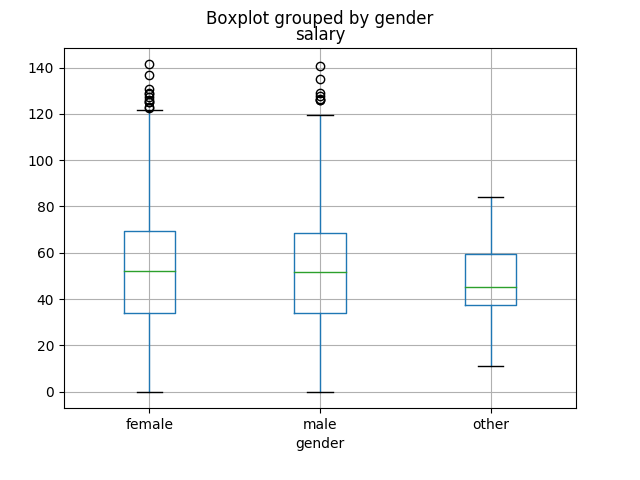
\includegraphics[width=0.45\textwidth]{genderSalary.png}
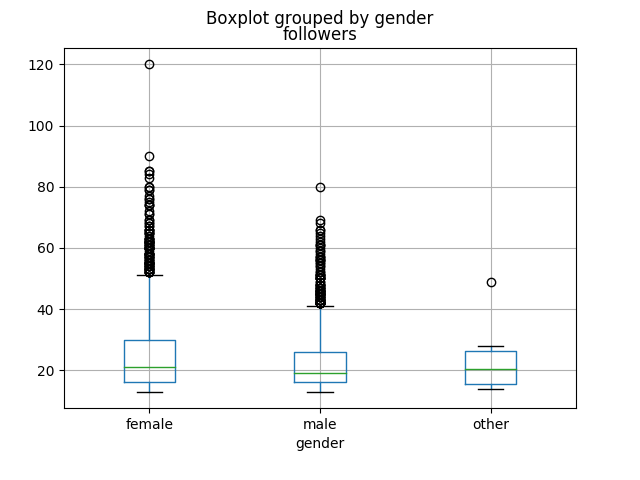
\includegraphics[width=0.45\textwidth]{genderFollowers.png}
\caption{Grouped box plots of salary (left) and number of social media
followers (right), grouped by gender.}
\label{fig:genderPlots}
\end{figure}

Similarly, we get the plot on the right-hand side with this code:

\begin{Verbatim}[fontsize=\small,samepage=true,frame=single,framesep=3mm]
people.boxplot('salary',by='followers')
\end{Verbatim}

This looks more skewed (\texttt{female}s appear to perhaps have more followers
on average than \texttt{male}s), but of course we won't know for sure until we
run the right statistical test.

\subsection{The $t$-test}

\index{t-test@\textit{t}-test}
\index{groupby@\texttt{.groupby()} method (Pandas)}
\index{bell-curvy@``bell-curvy''}

The test we'll use for significance here is called the \textbf{\textit{t}-test}
(sometimes ``Student's $t$-test'') and is used to determine whether the
\textit{means} of two groups are significantly different.\footnote{Strictly
speaking, the $t$-test assumes that the data sets you're comparing are ``bell
curvy'' (or ``normally distributed,'' to be precise) and we haven't checked for
that here. However, since we're doing \textit{exploratory} data analysis (not
drawing up and documenting final conclusions) it's common to use a $t$-test as
a quick-and-dirty just to see what's worth investigating.} Remember, we can get
the mean salary for each of the groups by using the \texttt{.groupby()} method:

\begin{Verbatim}[fontsize=\small,samepage=true,frame=single,framesep=3mm]
people.groupby('gender')['salary'].mean()
\end{Verbatim}
\vspace{-.2in}

\begin{Verbatim}[fontsize=\small,samepage=true,frame=leftline,framesep=5mm,framerule=1mm]
gender
female    52.031283
male      51.659983
other     48.757000
\end{Verbatim}

Females have the edge over males, 52.03 to 51.66. Our question is: is this
``enough'' of a difference to justify generalizing to the population?

To run the $t$-test, we first need a \texttt{Series} with just the
\texttt{male} salaries, and a different \texttt{Series} with just the
\texttt{female} salaries. These two \texttt{Series}es are \textit{not} usually
the same size. Let's use a query to get those:

\begin{Verbatim}[fontsize=\footnotesize,samepage=true,frame=single,framesep=3mm]
female_salaries = people[people.gender=="female"]['salary']
male_salaries = people[people.gender=="male"]['salary']
\end{Verbatim}
\vspace{-.2in}


\index{ttest\_ind@\texttt{ttest\_ind()} (SciPy)}

and then we can feed those as arguments to the \texttt{ttest\_ind()} function:

\begin{Verbatim}[fontsize=\small,samepage=true,frame=single,framesep=3mm]
scipy.stats.ttest_ind(female_salaries, male_salaries)
\end{Verbatim}
\vspace{-.2in}

\begin{Verbatim}[fontsize=\footnotesize,samepage=true,frame=leftline,framesep=5mm,framerule=1mm]
Ttest_indResult(statistic=0.52411385896, pvalue=0.60022263724)
\end{Verbatim}

This output is a bit more readable than the $\chi^2$ was. The second number in
that output is labeled ``\texttt{pvalue}'', which is over .05, and therefore we
conclude that \textit{there is no evidence that average salary differs between
males and females.}

Just to complete the thought, let's run this on the \texttt{followers} variable
instead:

\begin{Verbatim}[fontsize=\footnotesize,samepage=true,frame=single,framesep=3mm]
female_followers = people[people.gender=="female"]['followers']
male_followers = people[people.gender=="male"]['followers']
scipy.stats.ttest_ind(female_salaries, male_salaries)
\end{Verbatim}
\vspace{-.2in}

\begin{Verbatim}[fontsize=\footnotesize,samepage=true,frame=leftline,framesep=5mm,framerule=1mm]
Ttest_indResult(statistic=9.8614730266, pvalue=9.8573024317e-23)
\end{Verbatim}

\textbf{Warning!} When you first look at that $p$-value, you may be tempted to
say ``9.857 is \textit{waaay} greater than .05, so I guess this is a `no
evidence' result as well.'' Not so fast! If you look at the entire number --
including the ending -- you see:

\vspace{-.1in}
\begin{center}
\texttt{9.857302431746571e-23}
\end{center}
\vspace{-.1in}

\index{scientific notation}
\index{e@``\texttt{e}'' (exponential) notation}

that sneaky little ``\texttt{e-23}'' at the end is the kicker. This is how
Python displays numbers in \textbf{scientific notation} The
``\texttt{e}'' means ``times-ten-to-the.'' In mathematics, we'd write that
number as:

\vspace{-.2in}
\begin{center}
$9.857302431746571 \times 10^{-23}$
\end{center}
\vspace{-.2in}

which is:

\vspace{-.2in}
\begin{center}
$.000000000000000000000009857302431746571$
\end{center}
\vspace{-.2in}

Wow! That's clearly waaay \textit{less than} .05, and so we can say \textit{the
average number of followers \underline{does} depend significantly on the gender.}

Be careful with this. It's an easy mistake to make, and can lead to
embarrassingly wrong slides in presentations. \smiley

\subsubsection{More than two groups: ANOVA}

\index{ANOVA (ANalysis Of VAriance)}

By the way, the $t$-test is only appropriate when your categorical variable has
\textit{two} values (male vs.~female, for example, or vaccinated
vs.~non-vaccinated). If there are more than two, the appropriate test to run is
called an ``ANOVA'' (ANalysis Of VAriance). It's beyond the scope of this text,
but it's described in any intro stats textbook and is eminently Googleable.

\section{Two numeric variables}

Finally, we have the case where both variables are numeric. The \texttt{salary}
and \texttt{followers} columns are this case. Are they associated?

\subsection{Scatter plots}
\index{scatter plot}

The correct plot to visualize this is the \textbf{scatter plot}. It has an
axis for each numeric variable, and plots one dot (or other marker) for each
object of study: its $x$/$y$ coordinates depend on that object's value for each
variable.

The Pandas code is as follows:

\begin{Verbatim}[fontsize=\small,samepage=true,frame=single,framesep=3mm]
people.plot.scatter(x='followers',y='salary')
\end{Verbatim}

which produces Figure~\ref{fig:followersSalary}. Interestingly, there appear to
be a lot of people pegged at zero salary, and also at 10-ish followers. (These
observations would have shown up in a univariate analysis as well.) There's no
super obvious connection between the two variables, but if you squint at the
plot it (maybe) looks like there's a slight up-and-to-the-right trend, which
would indicate that having more followers is modestly associated with earning
more money.

\begin{figure}[ht]
\centering
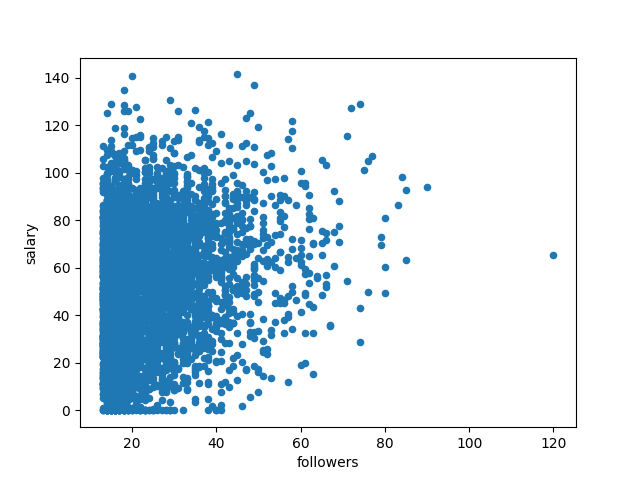
\includegraphics[width=0.8\textwidth]{followersSalary.png}
\caption{A scatter plot of \texttt{followers} vs.~\texttt{salary}. Each point
in the plot represents one person, with the $x$ and $y$ coordinates
corresponding to his/her/their number of followers and salary.}
\label{fig:followersSalary}
\end{figure}

\section{Pearson correlation coefficient}
\index{Pearson correlation coefficient}
\index{correlation coefficient}
\index{pearsonr@\texttt{pearsonr()} (SciPy)}

The test we'll use to see whether this pattern is significant is the
\textbf{Pearson correlation coefficient} (also called ``Pearson's $r$''). To
run it, we call SciPy's \texttt{pearsonr()} function and pass it the two
columns:

\begin{Verbatim}[fontsize=\small,samepage=true,frame=single,framesep=3mm]
scipy.stats.pearsonr(people.salary, people.followers)
\end{Verbatim}
\vspace{-.2in}

\begin{Verbatim}[fontsize=\small,samepage=true,frame=leftline,framesep=5mm,framerule=1mm]
(0.2007815176819964, 1.2285885030618397e-46)
\end{Verbatim}

We're given two numbers as output. The \textit{second} of these is the
$p$-value, and remembering our pitfall from above, we're savvy enough to notice
the \texttt{e-46} at the end and declare it significant. So we can say
\textit{we have high confidence that a person's salary is associated with their
number of social media followers.}

\index{positive correlation}
\index{negative correlation}

Now for the first number, which is the actual ``correlation coefficient.''
\textit{If} the second number is below $\alpha$ and therefore significant (as
it was here), you then look at the first number and see whether it's positive
or negative. Positive numbers indicate \textbf{positive correlations}: an
increase in one of the variables corresponds to an \textit{increase} in the
other. Negative numbers indicate \textbf{negative correlations}: an increase in
one of the variables corresponds to a \textit{decrease} in the other. Here, we
have a positive number, which means that \textit{having more followers tends to
go with a higher salary.}

As an example of the second (negative) case, suppose two of our variables in a
data set of sailboat races were \texttt{length} (the length of the sailboat,
from bow to stern) and \texttt{finish\_time} (the number of minutes the boat
took to complete the race). We're likely to see a negative correlation in this
case, because physics tells us that \textit{longer} boats can travel through
the water \textit{faster} (and therefore have \textit{lower} finish times).
These two variables would thus be correlated, but in a negative way: a high
value for one would typically indicate a \textit{low} value for the other.


\chapter{Branching}
\label{ch:branching}

\index{non-linear}
\index{branching}
\index{conditional execution}

In this chapter, we'll learn our next programming trick: how to execute code
\textit{conditionally}. This is called \textbf{branching}. It's another variant
of non-linear programming, like the loops from chapter~\ref{ch:loops}: it
enables something other than the strict, start-to-finish, line-by-line
execution of a program. In particular, branching allow us to designate certain
lines of code to be executed ``only sometimes.''

\section{The \texttt{if} statement}

\index{if statement@\texttt{if} statement}

The main branching statement in Python and most languages is the
\textbf{\texttt{if} statement}. Here's a couple of them in action:

\index{cash\_on\_hand@\texttt{cash\_on\_hand}}

\begin{Verbatim}[fontsize=\small,samepage=true,frame=single,framesep=3mm]
 1: name = "Horace"
 2: cash_on_hand = 100000
 3: IQ = 90
 4: print("Nice to meet you, {}!".format(name))
 5: if cash_on_hand > 5000:
 6:     print("Wow, you're rich! Gimme a fiver.")
 7:     cash_on_hand = cash_on_hand - 5
 8: if IQ > 100:
 9:     print("Wow, you're smart! Read a book.")
10:     IQ = IQ + 5
11: print("{}'s IQ is {} and he has ${}.".format(name, IQ, cash_on_hand))
\end{Verbatim}
\vspace{-.2in}

Even without any explanation, you might be able to figure out that the output
of the code snippet above is:

\begin{Verbatim}[fontsize=\small,samepage=true,frame=leftline,framesep=5mm,framerule=1mm]
Nice to meet you, Horace!
Wow, you're rich! Gimme a fiver.
Horace's IQ is 90 and he has $99995.
\end{Verbatim}

If not, stay tuned.

\index{loop!header}
\index{loop!body}
\index{indentation}

Just like a \texttt{for} loop, every \texttt{if} statement has a header and a
body. And just like a \texttt{for} loop, the determining factor of which lines
constitute the body depends on the indentation:

\begin{compactitem}
\item[\leftpointright] The first \texttt{if} statement's header is line \textbf{5}.
\item[\leftpointright] The first \texttt{if} statement's body is lines \textbf{6 and 7}.
\item[\leftpointright] The second \texttt{if} statement's header is line \textbf{8}.
\item[\leftpointright] The second \texttt{if} statement's body is lines
\textbf{9 and 10}.
\end{compactitem}

\index{condition (of an \texttt{if} statement)}

When an \texttt{if} statement is reached, its \textbf{condition} is evaluated;
in the first case, the condition ``\texttt{cash\_on\_hand > 500}'' is evaluated
to \texttt{True}, and in the second case, ``\texttt{IQ > 100}'' is determined
to be \texttt{False}. Then, \textit{only if} the condition is true will the
body of the \texttt{if} statement execute. Otherwise, it'll be skipped over.

Thus, the lines of the above program execute in this order: 1, 2, 3, 4, 5, 6,
7, 8, 11. Lines 9 and 10 are skipped entirely, since Horace's IQ wasn't above
average. Observe that the \texttt{cash\_on\_hand} variable was updated inside
the body of the first \texttt{if} statement, but that \texttt{IQ} was not.

\subsection{Compound conditions}

\index{compound condition}

Conditions can be more complicated than the ones above; just as with queries
(p.~\pageref{seriesCompoundQueries}) they can contain more than one component:

\begin{Verbatim}[fontsize=\small,samepage=true,frame=single,framesep=3mm]
if cash_on_hand > 10000 and IQ < 50:
    print("Wow, some dumb people are sure rich!")
\end{Verbatim}


You might have been surprised to see the word ``\texttt{and}'' in that
\texttt{if} statement instead of the character ``\texttt{\&}''. I feel you.
It's totally inconsistent, but nevertheless true: although in a query, you must
use the symbols \texttt{\&}, \texttt{|}, and \texttt{\textasciitilde}, in an
\texttt{if} condition, you must use the words \texttt{and}, \texttt{or}, and
\texttt{not}. (In other news, the bananas around the components of an
\texttt{if} condition aren't necessary, but you can include them if you want.)

\index{double-equals (\texttt{==})}
\index{==@\texttt{==} (double-equals)}

For your convenience, the \texttt{if} condition operators are listed in
Figure~\ref{fig:ifStatementOps}. (\textbf{Remember} the double-equals!!)

% in and .isin()

\begin{figure}[b]
\centering
\small
\bigskip
\begin{tabular}{c|c}
Operator & Meaning \\
\hline
\texttt{>} & greater than \\
\hline
\texttt{<} & less than \\
\hline
\texttt{>=} & greater than or equal to \\
\hline
\texttt{<=} & less than or equal to \\
\hline
\texttt{!=} & \textit{not} equal to \\
\hline
\texttt{==} & equal to \\
\hline
\texttt{and} & and \\
\hline
\texttt{or} & or \\
\hline
\texttt{not} & not \\
\end{tabular}

\bigskip
\normalsize
\caption{Operators in \texttt{if} statements: simple and compound.}
\label{fig:ifStatementOps}
\end{figure}

\section{The \texttt{if}/\texttt{else} statement}

\index{if/else statement@\texttt{if}/\texttt{else} statement}
\index{else}

The above examples execute the \texttt{if} body as long as the condition is
true, and do nothing otherwise. It's common to want to do something else in the
``otherwise'' case instead, and for that, we have the \texttt{if}/\texttt{else}
statement.

\begin{Verbatim}[fontsize=\footnotesize,samepage=true,frame=single,framesep=3mm]
name = "Gladys"
cash_on_hand = 2000
IQ = 120
print("Nice to meet you, {}!".format(name))
if cash_on_hand > 5000:
    print("Wow, you're rich! Gimme a fiver.")
    cash_on_hand = cash_on_hand - 5
else:
    print("I wish you well!")
if IQ > 100:
    print("Wow, you're smart! Read a book.")
    IQ = IQ + 5
else:
    print("You're currently not that smart, but read a book and get smarter.")
    IQ = IQ + 10
print("{}'s IQ is {} and she has ${}.".format(name, IQ, cash_on_hand))
\end{Verbatim}
\vspace{-.2in}

\begin{Verbatim}[fontsize=\small,samepage=true,frame=leftline,framesep=5mm,framerule=1mm]
Nice to meet you, Gladys!
I wish you well!
Wow, you're smart! Read a book.
Gladys's IQ is 125 and she has $2000.
\end{Verbatim}

You can see that ``\texttt{I wish you well!}'' was printed, since
\texttt{cash\_on\_hand} was \textit{not} greater than 5000 (as required by the
\texttt{if} condition), and that the ``\dots\texttt{you're smart!}\dots''
message was printed but not the ``\dots\texttt{not that smart}\dots'' one.
Both the \texttt{if} part and the \texttt{else} part have an indented body,
although only the \texttt{if} part has a condition.

And that brings up another point. Although it hardly seems worth mentioning,
let me nevertheless emphasize this oft-overlooked truth:

\definecolor{shadecolor}{rgb}{.9,.9,.9}
\begin{shaded}
Whenever an \texttt{if}/\texttt{else} statement is reached,
\textbf{\textit{either} the \texttt{if} body \textit{or} the \texttt{else}
body will always be executed. It's never both, and it's never neither one.}
\end{shaded}

This is always, always true, because of the nature of things. The reason the
\texttt{else} header doesn't have a condition is because its condition is
implicitly \textit{the exact opposite} of the \texttt{if} condition. Period. In
\textit{any} case where the \texttt{if} condition isn't true -- and
\textit{only} in such a case -- will the \textbf{else} condition be executed.

To test whether you fully understand this point, see if you can predict the
output of the following program, which 99\% of beginning programmers get wrong:

\begin{Verbatim}[fontsize=\small,samepage=true,frame=single,framesep=3mm]
name = "Javier"
lang = "French"

if lang == "Spanish":
    print("Hola, {}!".format(name))
if lang == "French":
    print("Bonjour, {}!".format(name))
if lang == "Chinese":
    print("Ni hao, {}!".format(name))
else:
    print("Hello, {}!".format(name))
\end{Verbatim}
\vspace{-.2in}

Seriously, don't feel bad if you miss this one. The answer (*drum roll please*)
is:

\begin{Verbatim}[fontsize=\small,samepage=true,frame=leftline,framesep=5mm,framerule=1mm]
Bonjour, Javier!
Hello, Javier!
\end{Verbatim}

Wait...wut? Why did it print two messages? Surely if \texttt{Javier}'s
preferred language is \texttt{French}, it ought to say ``\texttt{Bonjour}'' and
skip all the other options?

To understand this behavior, you have to realize that an
\texttt{if}/\texttt{else} statement is a \textit{single} entity. This
multi-lingual greeting program has three components:

\begin{samepage}
\begin{compactenum}
\item an \texttt{if} statement
\item an \texttt{if} statement
\item an \texttt{if}/\texttt{else} statement
\end{compactenum}
\end{samepage}

\index{golden rule}

And you must remember our golden rule in the shaded box:
\textbf{\textit{either} the \texttt{if} body \textit{or} the \texttt{else} body
will always be executed: never both, and never neither one.} Therefore, the
above program does this:

\begin{samepage}
\begin{compactenum}
\item If the language is Spanish, print an ``Hola'' message. (Otherwise, do
nothing.)
\item If the language is French, print a ``Bonjour'' message. (Otherwise, do
nothing.)
\item If the language is Chinese print a ``Ni hao'' message. Otherwise, print a
``Hello'' message.
\end{compactenum}
\end{samepage}

Once you recognize that structure, you'll realize that when step 3 is
encountered, the program \textit{must} print either ``Ni hao'' or ``Hello.'' It
can't print both, and it can't print neither. An \texttt{if}/\texttt{else} just
doesn't work any other way.

\section{The \texttt{if}/\texttt{elif}/\texttt{else} statement}

\index{if/elif/else statement@\texttt{if}/\texttt{elif}/\texttt{else} statement}
\index{elif}

The problem with the previous example is that we really want our four languages
to be \textbf{mutually exclusive} options. If \texttt{lang} is
\texttt{"Spanish"}, we want it to print ``Hola'' and skip all the rest. The
easiest way to get this behavior is to use ``\texttt{elif}'' (a horrid
abbreviation of the phrase ``else if'').

Squint hard at this program until you see the differences between it and the
previous one:

\begin{Verbatim}[fontsize=\small,samepage=true,frame=single,framesep=3mm]
name = "Javier"
lang = "French"

if lang == "Spanish":
    print("Hola, {}!".format(name))
elif lang == "French":
    print("Bonjour, {}!".format(name))
elif lang == "Chinese":
    print("Ni hao, {}!".format(name))
else:
    print("Hello, {}!".format(name))
\end{Verbatim}

It's identical except that we replaced the second two \texttt{if}'s with
\texttt{elif}'s. This tells Python: only if the language is \textit{not}
Spanish should you then consider whether or not it's French. And only if it's
\textit{not} French (and \textit{not} Spanish) should you consider whether or
not it's Chinese. And only if it's not Chinese (and not French (and not
Spanish)) should you print ``Hello.''

Whether to use sequential \texttt{if}s or a chain of \texttt{elif}s isn't
always an easy question to answer. Neither choice is always right: you have to
think rigorously logically about how the program should act. Ask yourself: ``do
I want Python to consider \textit{all} of these conditions -- and execute the
appropriate \texttt{if} bodies -- no matter what? Or do I want it to bail out
as soon as it finds one that's true?'' Like most things, it takes practice to
get right.


% nested

% loops


\chapter{Functions}
\label{ch:functions}

\index{function}
\index{writing a function@writing a function}
\index{non-linear}

And now for the very last ``pure programming'' lesson of the book: writing
\textbf{function}s. This is more or less the final tool in the programmer's
toolkit, and as I've learned over my years of teaching, it often causes the
most trouble.

Now you might be thinking, ``hey waitaminit, we've known about functions since
all the way back on p.~\pageref{function}. This is something new?'' Yes it is.
Previously in this book, we've done a lot of \textit{calling} functions -- from
\texttt{len()} to \texttt{np.append()} to \texttt{pd.read\_csv()} to
\texttt{scipy.stats.chi2\_contingency()} -- that someone else has written for
us. In this chapter, we look behind the curtain and join the production staff:
we write our \textit{own} functions.

\section{Why do all this}

It turns out there's a lot of syntactic nonsense involved to get all the wiring
right when you do this. It can cause students to pull their hair out. So it's
worth asking at the outset: what do we get for all this pain?

\index{modular}

The answer is subtle, and can seem underwhelming at first, but it's crucial. It
essentially boils down to this lesson: any complex creative work (including a
computer program) should be \textbf{modular} in its design. This means that it
should be composed of smaller building blocks, which are in turn composed of
smaller building blocks, and that the whole thing should comprise an organized
whole.

Any other way of doing it leads to madness.

\index{car engine}

Think of a car engine. When a mechanic opens up the hood, he or she doesn't see
just one big monolithic thing called ``The Engine,'' but rather piston
assemblies, spark plugs, water pumps, drive shafts, and lots of other
subsystems. It's what allows piece by piece investigation of problems, and
piece by piece replacement of bad parts.

\index{creativity}
\index{rock 'n' roll}

Or think of a rock 'n' roll tune. It's not just an impenetrable mass of sound.
Instead, it's a collection of recognizable bass lines, drum sequences, vocal
patterns, and variations on common guitar riffs. This isn't to minimize the
creativity involved in its orchestration; in fact, the novel combination of the
myriad possible building blocks \textit{is} the creativity. If it were just an
impermeable wall of sound, it would be noise, not music.

% TODO Susan Polgar
% I like to tell the story of Susan Polgar, and the ``simul'' match I saw her
% play.

\index{spaghetti code@``spaghetti code''}

In the same way, once your data analysis code approaches a certain size, it
really must be written in a modular way or it will become a hopelessly tangled
mess, what programmers refer to as ``spaghetti code.'' And the way to achieve
this is by writing it in terms of functions that you then call at the
appropriate time.

\index{reusable}
\index{wheel, reinventing}

One other advantage to this approach, by the way, is that functions are
\textbf{reusable}. Think of how many different programmers all over the world
have had reason to call \texttt{np.sort()}, or \texttt{scipy.stats.pearsonr()}!
The same function becomes applicable in a variety of different contexts, so
that nobody has to reinvent the wheel.

\section{The \texttt{def} statement}

\index{def statement@\texttt{def} statement}

Okay, down to brass tacks.


\chapter{Functions (2 of 2)}

Like many things in life, writing functions is best learned by example. This
chapter will feature several more of them that you can learn from and imitate.

\subsubsection{Basketball scoring: \texttt{bb\_pts()}}

Continuing the sports theme, the total points a basketball player scores is
related to the number of shots she makes of various kinds. Typically, the ``box
score'' of a game (see example in Figure~\ref{boxScore}) reports three scoring
stats: (1) the \textit{total} number of ``field goals''\footnote{A ``field
goal'' in basketball just means ``a regular basket'' -- \textit{i.e.}, not a
free throw penalty shot.} a player made and attempted, (2) the number of these
field goals, if any, that were for three points\footnote{In most leagues, a
basket is worth 2 points unless the shooter was farther than a certain distance
from the hoop when she shot it, in which case it's worth 3.}, and (3) the
number of free throws (``easy'' penalty shots) the player attempted and made.

Confusingly, (1) \textit{includes} (2). In other words, if the first number is
4 and the second is 1, the player didn't score 4 regular two-point baskets and
1 three-pointer, but rather \textit{3} two-point baskets and 1 three-pointer.

\begin{figure}[ht]
\centering
\fbox{
\mbox{
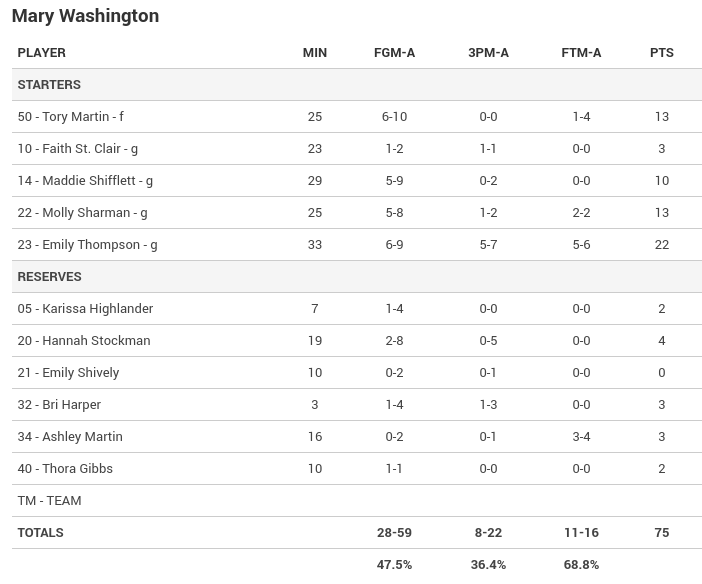
\includegraphics[width=0.8\textwidth]{boxScore.png}
}
}
\medskip
\caption{A basketball box score.}
\label{boxScore}
\end{figure}

In Figure~\ref{boxScore}, the \textsf{FGM-A} column gives the first of these
three categories, \textsf{3PM-A} the second, and \textsf{FTM-A} the third. The
\textsf{PTS} column gives the total number of points that player scored. (For
example, Molly Sharman made 5 of her 8 attempted field goals, one of which was
for three points, and she also converted both free throw attempts.)

All that took a lot longer to explain than the corresponding Python function:

\index{bb\_pts@\texttt{bb\_pts()}}

\begin{Verbatim}[fontsize=\footnotesize,samepage=true,frame=single,framesep=3mm]
def bb_pts(fgm, threep_fgm, ftm):
    return ((fgm - threep_fgm) * 2) + (threep_fgm * 3) + ftm

torys_pts = bb_pts(6, 0, 1)
print("Tory scored {} points.".format(torys_pts))
print("Emily scored {} points.".format(bb_pts(6,5,5)))
print("Lady Eagles scored {} points!".format(bb_pts(28,8,11)))
\end{Verbatim}
\vspace{-.2in}

\begin{Verbatim}[fontsize=\small,samepage=true,frame=leftline,framesep=5mm,framerule=1mm]
Tory scored 13 points.
Emily scored 22 points.
Lady Eagles scored 75 points!
\end{Verbatim}

\index{PEMDAS}

Strictly speaking you don't need all those bananas (regular PEMDAS
order-of-operations applies) but I think it's a good idea to include them for
clarity and grouping.

\subsubsection{``Exceptions'': \texttt{mean\_no\_outliers()} and \texttt{quiz\_avg()}}

Sometimes we want to take the straight average of a data set, but other times
we may want to filter out any strange or exceptional cases. Let's say we're
computing the average age of a classroom of college students, but we want to
remove any adult learners over 30 since that would skew the result. We could do
this sort of thing with a function like this:

\index{mean\_no\_outliers@\texttt{mean\_no\_outliers()}}
\index{low\_cutoff@\texttt{low\_cutoff}}
\index{high\_cutoff@\texttt{high\_cutoff}}

\begin{Verbatim}[fontsize=\footnotesize,samepage=true,frame=single,framesep=3mm]
def mean_no_outliers(a, low_cutoff, high_cutoff):
    return a[(a >= low_cutoff) & (a <= high_cutoff)].mean()

our_class = np.array([20,18,19,18,22,21,76,20,22,22,21,18])
print("The average age (excluding outliers) is {}.".format(
    mean_no_outliers(our_class, 0, 30)))
\end{Verbatim}

\vspace{-.2in}

\begin{Verbatim}[fontsize=\small,samepage=true,frame=leftline,framesep=5mm,framerule=1mm]
The average age (excluding outliers) is 20.09090909090909.
\end{Verbatim}

We've provided two arguments to the function besides the data set itself: a
lower and upper bound. Anything falling outside that range will be filtered
out. In the example function call, we passed 0 for the \texttt{low\_cutoff}
since we didn't desire to filter anything at the low end. (If we wanted to,
say, also remove children from the data set, we could have set that to 16 or
so.)

By the way, you might find the number of decimal places printed to be
unsightly. If so, we could enhance our function by rounding the result to (say)
two decimals with NumPy's \texttt{round()} function:

\index{round@\texttt{round()} function (NumPy)}
\label{round}

\begin{Verbatim}[fontsize=\footnotesize,samepage=true,frame=single,framesep=3mm]
def mean_no_outliers(a, low_cutoff, high_cutoff):
    return np.round(a[
        (a >= low_cutoff) & (a <= high_cutoff)].mean(),2)

print("The average age (excluding outliers) is {}.".format(
    mean_no_outliers(our_class, 0, 30)))
\end{Verbatim}
\vspace{-.2in}

\begin{Verbatim}[fontsize=\small,samepage=true,frame=leftline,framesep=5mm,framerule=1mm]
The average age (excluding outliers) is 20.09.
\end{Verbatim}

At this point you might think this function is getting pretty big for a
one-liner. I agree. Let's split it up and use some temporary variables to make
it more readable:

\begin{Verbatim}[fontsize=\footnotesize,samepage=true,frame=single,framesep=3mm]
def mean_no_outliers(a, low_cutoff, high_cutoff):
    filtered_data = a[(a >= low_cutoff) & (a <= high_cutoff)]
    filtered_average = np.round(filtered_data)
    return np.round(filtered_average,2)
\end{Verbatim}

Much clearer!

\medskip

A related but different example would be to remove a fixed \textit{number} of
data points from the end, instead of data points outside a specified range. For
instance, in my classes, I often give students (say) eight quizzes during a
semester, and drop the lowest two scores. That could be done with:

\index{sorting@sorting (arrays)}
\index{sort@\texttt{np.sort()} (NumPy)}
\index{quiz\_avg@\texttt{quiz\_avg()}}
\index{Filbert}

\begin{Verbatim}[fontsize=\footnotesize,samepage=true,frame=single,framesep=3mm]
def quiz_avg(quizzes):
    dropped_lowest_two = np.sort(quizzes)[2:len(quizzes)]
    return dropped_lowest_two.mean()

filberts_quizzes = np.array([7,9,10,7,0,8,4,10])
print("Filbert's avg score was {}.".format(quiz_avg(
    filberts_quizzes)))
\end{Verbatim}
\vspace{-.2in}

\begin{Verbatim}[fontsize=\small,samepage=true,frame=leftline,framesep=5mm,framerule=1mm]
Filbert's avg score was 8.5.
\end{Verbatim}

Filbert's 0 and 4 were dropped, leaving him with a pretty good semester score.

The trick to this implementation is \textit{sorting} the quiz scores. Once you
do that, it's easy to pick out the top six to take the average, since the
lowest two scores will be at the beginning of the (sorted) array. Two notes
here:


% TODO: actually do slices in chapter arraysInPython1.

\begin{compactitem}

\item We use the \texttt{np.sort()} function, not the \texttt{.sort()} method,
since we don't want to permanently change the order of \texttt{quizzes}. We
only need a temporarily sorted copy so we can omit the lowest two entries.

\index{slice}
\index{boxies (square brackets)}
\index{[]@\texttt{[]} (boxies)}

\item That business in the boxies (``\texttt{[2:len(quizzes)]}'') is a
\textbf{slice} (recall chapter~\ref{ch:arraysInPython1}) which says ``only give
me entries number 2 through the end of the array.'' And that's exactly what the
doctor ordered to omit the first two.
\end{compactitem}

\smallskip

\subsubsection{Searching for values: \texttt{any\_zeros()}}

I'll end this chapter with an example which, like the ``preferred language''
example on p.~\pageref{spanishFrenchPitfall}, flummoxes nearly every beginning
student.

Suppose students in a DATA 101 course are given labs to complete, each one
worth up to 20 points. (This is purely hypothetical, as you can see.) At the
midway point of the semester, the instructor would like a quick list of any
students who failed to turn in one of the labs, so he can harass them for their
own good.

\index{Filbert}
\index{Betty Lou}
\index{Jezebel}
\index{Biff}
\index{Melvin}
\index{gradebook@\texttt{gradebook}}

Here's the \texttt{gradebook} \texttt{DataFrame} this professor is using:

\begin{Verbatim}[fontsize=\footnotesize,samepage=true,frame=leftline,framesep=5mm,framerule=1mm]
           Q1  Q2  Q3  Q4  lab1  lab2  lab3  lab4  lab5
student                                                
Filbert     7   9  10   7    15    19    14    20    20
Jezebel     8   7   0   6    12    12    16     0    20
Betty Lou  10  10  10  10    20    20    20    20    20
Biff        3   2   6   5    10    12     0     0    16
Melvin      0   0  10  10     0    18    20    14    20
\end{Verbatim}

\index{print\_harass\_list@\texttt{print\_harass\_list()}}

Let's write a function called \texttt{print\_harass\_list()} whose job is to
tell this professor which students he should check up on. We'll write it as
follows:

\begin{Verbatim}[fontsize=\footnotesize,samepage=true,frame=single,framesep=3mm]
def print_harass_list(gradebook):
    for row in gradebook.itertuples():
        if any_zeros(np.array([row.lab1, row.lab2, row.lab3,
            row.lab4, row.lab5])):
            print("Better check up on {}.".format(row.Index))
\end{Verbatim}

\index{iteration}

\index{any\_zeros@\texttt{any\_zeros()}}
Note that we've pushed some of the work on to a new function,
\texttt{any\_zeros()}, that we haven't written yet. This is good organizational
style. Now \texttt{print\_harass\_list()} can do the job of iterating through
the \texttt{DataFrame} rows, extracting the lab scores, and printing a message
if necessary, whereas it defers to \texttt{any\_zeros()} to inspect the lab
scores and determine the presence of any zeros.

It doesn't work until we actually write the second function, of course, so here
goes. Heads up, since this is the part that perplexes students. The following
implementation of \texttt{any\_zeros()} looks perfectly reasonable, yet is dead
WRONG:

\begin{Verbatim}[fontsize=\small,samepage=true,frame=single,framesep=3mm]
def any_zeros_WRONG(labs):
    for lab in labs:
        if lab == 0:
            return True
        else:
            return False
\end{Verbatim}

It looks so correct! And yet it is not. Check out the result:

\begin{Verbatim}[fontsize=\small,samepage=true,frame=single,framesep=3mm]
print_harass_list(gradebook)
\end{Verbatim}
\vspace{-.2in}

\begin{Verbatim}[fontsize=\small,samepage=true,frame=leftline,framesep=5mm,framerule=1mm]
Better check up on Melvin.
\end{Verbatim}

Clearly we need to check up on \texttt{Jezebel} and \texttt{Biff} as well (look
at their scores for labs 3 and 4), yet they inexplicably didn't get printed.

\index{cardinal rule@cardinal rule (of \texttt{if}/\texttt{else})}

Here's what's WRONG with that \texttt{any\_zeros()} attempt. Stare carefully at
that loop and realize that the \textit{body} of the loop is comprised of a
single \texttt{if}/\texttt{else} statement. And remember our cardinal rule from
the grey box on p.~\pageref{cardinalRule}: either the \texttt{if} body or the
\texttt{else} body will \textit{always} be executed.

That means that this loop is destined to only execute exactly once! It doesn't
matter how long the \texttt{labs} array is. It effectively looks only at the
\textit{first} element, and decides based solely on that whether or not the
entire array has any zeros in it!

\index{any\_zeros@\texttt{any\_zeros()}}
The correct version of \texttt{any\_zeros()} would look like this:

\begin{Verbatim}[fontsize=\small,samepage=true,frame=single,framesep=3mm]
def any_zeros(labs):
    for lab in labs:
        if lab == 0:
            return True
    return False
\end{Verbatim}

\index{indentation}

At first glance, it may appear unchanged, but look again. First of all, there's
no \texttt{else} anymore. Second of all, the ``\texttt{return False}'' line is
indented \textit{evenly with the word \texttt{for}}. This means that
``\texttt{return False}'' is \textit{not} part of the loop at all: it will only
run \textit{after} the entire loop has executed.

That turns out to make all the difference. The function will dutifully go
through \textit{each} element of the \texttt{labs} array, inspecting each one
to see whether it's zero. As soon as it finds a zero, it returns \texttt{True},
since then its job is done. Only after inspecting the \textit{entire} array,
and coming up empty on its zero quest, does this function then have the
audacity to return \texttt{False}, meaning ``nope! Clean as a whistle.'' The
result:

\begin{Verbatim}[fontsize=\small,samepage=true,frame=leftline,framesep=5mm,framerule=1mm]
Better check up on Jezebel.
Better check up on Biff.
Better check up on Melvin.
\end{Verbatim}

\subsubsection{Postlude: thinking algorithmically}

\index{algorithmic thinking}
\index{holistic thinking}
\index{thinking algorithmically vs.~holistically}

Getting tripped up on that last example is, I believe, usually a case of
\textit{thinking holistically} rather than \textit{thinking algorithmically}.
Math classes have trained people to think holistically, by which I mean looking
at (say) a bunch of equations and viewing them as ``all equally true, all at
once.'' And this is the correct way to think mathematically. If I give you five
simultaneous equations that state relationships among variables, they aren't
really in any order. They're just ``five true things.''

But programming requires you to think algorithmically. You have to execute the
code in your head, step by step, and realize the consequences. The appealing
symmetry of the WRONG \texttt{any\_zeros()} function is appealing because
you're looking at it as a whole: ``it's looping (seemingly) through all the
elements, with zeros being an indicator of \texttt{True}ness and non-zeros
being an indicator of \texttt{False}ness. What's not to like?'' The error, as
you saw, is that when running through the data step-by-step, there are immense
ramifications of returning early. That's only apparent if you think of the code
executing sequentially as it goes. You have to pretend you're the computer, not
a mathematician.

% Other examples:
% def is_tall(ht_ft, ht_in, sex):
%    inches_tall = ht_ft * 12 + ht_in
%    if sex == "male":
%        if inches_tall > 70:
%            return True
%        else:
%            return False
%    else:
%        if inches_tall > 64:
%            return True
%        else:
%            return False


\chapter{Recoding and transforming}

It's often the case that although a \texttt{DataFrame} contains the raw
information you need, it's not exactly in the form you need for your analysis.
Perhaps the data is in different units than you need -- meters instead of feet;
dollars instead of yen. Or perhaps you need some \textit{combination} of
available quantities -- miles per gallon instead of just miles and gallons
separately. Or perhaps you need to reframe a variable by binning it into
meaningful subdivisions -- categorizing a raw column of salaries into ``high,''
``medium,'' and ``low'' wage earners, for instance.

\index{derived column}
\index{column (of a table)}

In data science, these activities are known as \textbf{recoding} and/or
\textbf{transforming}. There's not a sharp division between the two; usually I
think of recoding as converting a single variable to one with different units
(as in the dollars-to-yen and high/medium/low earners examples) and
transforming as creating a new variable entirely out of a combination of
columns (like miles per gallon). In both cases, though, we'll be creating and
adding new columns to a \texttt{DataFrame}. These columns are sometimes called
\textbf{derived columns} since they're based on (derived from) existing columns
rather than containing independent information.

\section{Recoding with simple operations}

\index{soccer}
\index{US Women's National Team}

Consider the following soccer data set called \texttt{worldcup2019.csv}.
Each row of this data set represents one player's performance in a particular
2019 World Cup game. Notice that we have a couple of players with more than one
row (Megan Rapinoe and Rose Lavelle), and several rows for the same game (the
first four rows are all from the June 28th game, for instance):

\begin{Verbatim}[fontsize=\small,samepage=true,frame=lines,framesep=3mm]
last,first,date,in_time,out_time,goals,asst,tackles,shots
Morgan,Alex,28-Jun-2019,0.0,90.0,0,0,2,1
Rapinoe,Megan,28-Jun-2019,0.0,74.0,2,0,2,3
Press,Christen,28-Jun-2019,74.0,90.0,0,0,1,0
Lavelle,Rose,28-Jun-2019,0.0,90.0,0,1,3,0
Lavelle,Rose,7-Jul-2019,0.0,90.0,1,0,4,1
Rapinoe,Megan,7-Jul-2019,0.0,83.0,1,1,3,2
Lloyd,Carli,7-Jul-2019,87.0,90.0,0,0,1,0
Dunn,Crystal,23-Jun-2019,42.0,81.0,0,1,1,2
\end{Verbatim}

\index{set\_index@\texttt{.set\_index()} method (Pandas)}

The data set doesn't really have a meaningful index column, since none of the
columns are expected to be unique. So we'll leave off the
``\texttt{.set\_index()}'' method call when we read it in to Python:

\begin{samepage}
\begin{Verbatim}[fontsize=\footnotesize,samepage=true,frame=single,framesep=3mm]
wc = pd.read_csv('worldcup2019.csv')
print(wc)
\end{Verbatim}
\vspace{-.2in}

\begin{Verbatim}[fontsize=\scriptsize,samepage=true,frame=leftline,framesep=5mm,framerule=1mm]
     last    first   date in_mins in_secs out_mins out_secs goals asst tackles shots
0  Morgan     Alex 28-Jun       0       0       90        0     0    0       2     1
1 Rapinoe    Megan 28-Jun       0       0       74       27     2    0       2     3
2   Press Christen 28-Jun      74      27       90        0     0    0       1     0
3 Lavelle     Rose 28-Jun       0       0       90        0     0    1       3     0
4 Lavelle     Rose  7-Jul       0       0       90        0     1    0       4     1
5 Rapinoe    Megan  7-Jul       0       0       83       16     1    1       3     2
6   Lloyd    Carli  7-Jul      83      16       90        0     0    0       1     0
7    Dunn  Crystal 23-Jun      42      37       81        5     0    1       1     2
\end{Verbatim}
\end{samepage}

(As you can see, Pandas put in a numeric index column for us.)

Let's zero in on the columns with \texttt{mins} and \texttt{secs} in the names.
These columns show us the minute and second that the player went \texttt{in} to
the game, and the minute and second that they came \texttt{out}. For example,
Alex Morgan played the entire 90-minute match on June 28th. Rapinoe started
that game, but came out for a substitute at the 74:27 mark. Who replaced her?
Looks like Christen Press did, since she \textit{entered} the game at exactly
the same time. In most rows, the player either started the game, or ended the
game or both, but the last row (Crystal Dunn's June 23rd performance) has her
entering at 42:37 and exiting at 81:05.

Now the reason I bring this up is because one aspect of our analysis might be
computing statistics \textit{per minute} that each athlete played. If one
player scored 3 goals in 200 minutes, for example, and another scored 3 goals
in just 150 minutes, we could reasonably say that the second player was a more
prolific scorer in that World Cup.

\index{recoding}
\index{round@\texttt{round()} function (NumPy)}

This is hard to do with the data in the form that it stands. So we'll
\textbf{recode} a few of the columns. Let's collapse the minutes and seconds
for each of the two clock times into a single value, in minutes. For
readability, we'll also round this number to two decimal places using the
\texttt{round()} function we met on p.~\pageref{round}:

\begin{Verbatim}[fontsize=\small,samepage=true,frame=single,framesep=3mm]
wc['in_time'] = np.round(wc['in_mins'] + (wc['in_secs'] / 60),2)
wc['out_time'] = np.round(wc['out_mins'] + (wc['out_secs'] / 60),2)
\end{Verbatim}

\index{vectorized@``vectorized'' operation}

We're taking advantage of vectorized operations here. For each row, we need to
divide the \texttt{in\_secs} value by 60 (to convert it to minutes) and add it
to the \texttt{in\_mins} value. Pandas makes this super easy here, since we can
just write out those operations once, and it will compute it for every single
row!

\medskip
Let's delete the old, superfluous columns now and see what we've got:

\begin{samepage}
\begin{Verbatim}[fontsize=\small,samepage=true,frame=single,framesep=3mm]
del wc['in_mins']
del wc['in_secs']
del wc['out_mins']
del wc['out_secs']
print(wc)
\end{Verbatim}
\vspace{-.2in}

\begin{Verbatim}[fontsize=\footnotesize,samepage=true,frame=leftline,framesep=5mm,framerule=1mm]
     last    first   date goals asst tackles shots in_time out_time
0  Morgan     Alex 28-Jun     0    0       2     1    0.00    90.00
1 Rapinoe    Megan 28-Jun     2    0       2     3    0.00    74.45
2   Press Christen 28-Jun     0    0       1     0   74.45    90.00
3 Lavelle     Rose 28-Jun     0    1       3     0    0.00    90.00
4 Lavelle     Rose  7-Jul     1    0       4     1    0.00    90.00
5 Rapinoe    Megan  7-Jul     1    1       3     2    0.00    83.27
6   Lloyd    Carli  7-Jul     0    0       1     0   83.27    90.00
7    Dunn  Crystal 23-Jun     0    1       1     2   42.62    81.08
\end{Verbatim}
\end{samepage}

This is much less unwieldy than dealing with minutes and seconds separately.

% TODO: give warning about changing the values of an existing DF column -- you
% get the weird "changing on a slice/copy of a DF" warning, which sometimes
% means it doesn't work. 

\section{Transforming with simple operations}

\index{transforming}

\index{mins\_played@\texttt{mins\_played}}

Now that we've converted the awkward minutes-and-seconds columns to just
``\texttt{time}'' columns, all we need to do to complete our analysis is
\textbf{transform} this data by computing a new quantity entirely: the
\textit{total number of minutes played} for each player in each game. Again,
Pandas makes this easy:

\begin{Verbatim}[fontsize=\small,samepage=true,frame=single,framesep=3mm]
wc['mins_played'] = wc.out_time - wc.in_time
print(wc)
\end{Verbatim}
\vspace{-.2in}

\begin{Verbatim}[fontsize=\footnotesize,samepage=true,frame=leftline,framesep=5mm,framerule=1mm]
     last    first   date goals asst tackles shots in_time out_time mins_played
0  Morgan     Alex 28-Jun     0    0       2     1    0.00    90.00       90.00
1 Rapinoe    Megan 28-Jun     2    0       2     3    0.00    74.45       74.45
2   Press Christen 28-Jun     0    0       1     0   74.45    90.00       15.55
3 Lavelle     Rose 28-Jun     0    1       3     0    0.00    90.00       90.00
4 Lavelle     Rose  7-Jul     1    0       4     1    0.00    90.00       90.00
5 Rapinoe    Megan  7-Jul     1    1       3     2    0.00    83.27       83.27
6   Lloyd    Carli  7-Jul     0    0       1     0   83.27    90.00        6.73
7    Dunn  Crystal 23-Jun     0    1       1     2   42.62    81.08       38.46
\end{Verbatim}

\index{tackles-per-game}
\index{tkl\_per\_90@\texttt{tkl\_per\_90}}

Voil\`{a}. We now have the time-on-field for each player, which gives us a
whole new avenue of exploration. For example, any of the counting stats (goals,
assists, \textit{etc.}) can be converted into a ``per-minute'' version, showing
us how productive a player was while on the field. Let's do that for
\texttt{tackles}, and multiply by 90 to obtain a ``tackles-per-90-minutes''
statistic\footnote{I'm choosing 90 minutes here because that's how long a
regulation-length soccer match is. Therefore, our new \texttt{tkl\_per\_90}
column gives us ``number-of-tackles-per-complete-game,'' which is easier to
interpret than ``tackles-per-\textit{minute},'' which would be a miniscule
number for any player.}:

\begin{Verbatim}[fontsize=\small,samepage=true,frame=single,framesep=3mm]
wc['mins_played'] = wc['out_time'] - wc['in_time']
wc['tkl_per_90'] = np.round(wc['tackles'] / wc['mins_played'] * 90,2)
del wc['tackles']
\end{Verbatim}
\vspace{-.2in}

\begin{Verbatim}[fontsize=\footnotesize,samepage=true,frame=leftline,framesep=5mm,framerule=1mm]
     last    first   date goals asst shots in_time out_time mins_played tkl_per_90
0  Morgan     Alex 28-Jun     0    0     1    0.00    90.00       90.00       2.00
1 Rapinoe    Megan 28-Jun     2    0     3    0.00    74.45       74.45       2.42
2   Press Christen 28-Jun     0    0     0   74.45    90.00       15.55       5.79
3 Lavelle     Rose 28-Jun     0    1     0    0.00    90.00       90.00       3.00
4 Lavelle     Rose  7-Jul     1    0     1    0.00    90.00       90.00       4.00
5 Rapinoe    Megan  7-Jul     1    1     2    0.00    83.27       83.27       3.24
6   Lloyd    Carli  7-Jul     0    0     0   83.27    90.00        6.73      13.37
7    Dunn  Crystal 23-Jun     0    1     2   42.62    81.08       38.46       2.34
\end{Verbatim}

\subsection{Transforming grouped data}

The above example computed tackles-per-game all right, but it still left us
with one row for every player-performance. (In other words, the results had
\textit{two} rows for Rose Lavelle, one giving her \texttt{tkl\_per\_90} for
the June 28th game, and one giving it for the July 7th game.)

\index{groupby@\texttt{.groupby()} method (Pandas)}

We might instead be interested in a player-by-player analysis: overall in the
entire month-long World Cup, which players had the most tackles-per-game? This
is easy to do with the \texttt{.groupby()} method that we first encountered in
section~\ref{groupby} (p.~\pageref{groupby}). First, we group the rows by the
first \textit{two} columns (since first-and-last-names-together are needed to
uniquely identify a single player):

\index{grouped\_wc@\texttt{grouped\_wc}}

\begin{Verbatim}[fontsize=\footnotesize,samepage=true,frame=single,framesep=3mm]
grouped_wc = wc.groupby(['last','first'])
\end{Verbatim}

We then take our new, temporary \texttt{grouped\_wc} variable and extract the
\texttt{goals}, \texttt{asst}, \texttt{shots}, \texttt{tackles}, and
\texttt{mins\_played} columns from it, \textbf{summing} each of them to produce
the per-player values in the result:

\index{by\_player@\texttt{by\_player}}

\begin{Verbatim}[fontsize=\footnotesize,samepage=true,frame=single,framesep=3mm]
by_player = grouped_wc[['goals','asst','shots','tackles','mins_played']].sum()
\end{Verbatim}

This yields:

\begin{Verbatim}[fontsize=\small,samepage=true,frame=leftline,framesep=5mm,framerule=1mm]
                  goals  asst  shots  tackles  mins_played
last    first                                             
Dunn    Crystal       0     1      2        1        38.46
Lavelle Rose          1     1      1        7       180.00
Lloyd   Carli         0     0      0        1         6.73
Morgan  Alex          0     0      1        2        90.00
Press   Christen      0     0      0        1        15.55
Rapinoe Megan         3     1      5        5       157.72
\end{Verbatim}

Now, we're ready to compute a per-game analysis as before, but this time for
each player's entire World Cup games:

\begin{Verbatim}[fontsize=\small,samepage=true,frame=single,framesep=3mm]
by_player['tkl_per_90'] = (np.round(by_player['tackles'] /
    by_player['mins_played'] * 90,2))
del by_player['tackles']
\end{Verbatim}
\vspace{-.2in}

\begin{Verbatim}[fontsize=\small,samepage=true,frame=leftline,framesep=5mm,framerule=1mm]
                  goals  asst  shots  mins_played  tkl_per_90
last    first                                                
Dunn    Crystal       0     1      2        38.46        2.34
Lavelle Rose          1     1      1       180.00        3.50
Lloyd   Carli         0     0      0         6.73       13.37
Morgan  Alex          0     0      1        90.00        2.00
Press   Christen      0     0      0        15.55        5.79
Rapinoe Megan         3     1      5       157.72        2.85
\end{Verbatim}

\section{Transforming with more complex operations}

\index{vectorized@``vectorized'' operation}

In all the above examples, we took advantage of Pandas vectorized operations.
With just a single line of code like ``\texttt{wc[\textquotesingle
mins\_played\textquotesingle] = wc.out\_time - wc.in\_time}'', we could compute
our entire new transformed column in one fell swoop.

\index{loop}

Sometimes, we're not so lucky. In particular, if the computation of the
transformed column is more complicated than just numeric operations -- like, if
it involves branches, loops, or calling other functions -- we normally can't
compute it all at once. Instead, we have to resort to a loop.

Pandas makes this procedure a bit awkward in my opinion. But once you learn the
pattern, it's not hard to imitate. Here's the pattern for creating a
transformed/recoded column that requires more complex operations:

\definecolor{shadecolor}{rgb}{.9,.9,.9}
\begin{shaded}
\begin{compactenum}
\item Create a \textbf{function} that will compute the transformed value for a
\textit{single} row. Its arguments should be whatever column values are
necessary to derive the new value, and its return value should be the desired
transformation.
\item Create an \textit{empty} NumPy array to hold the row-by-row results, and
make sure it's the right type.
\item Write a loop that will iterate through all the rows of the original
\texttt{DataFrame}. For each row, pass the appropriate values to the function,
and then \textit{append} the return value to the ever-growing NumPy array.
\item Finally, slap that NumPy array on to the \texttt{DataFrame} as a new
column.
\end{compactenum}

\end{shaded}

Here's a couple examples. First, suppose we want to compute a shooting
percentage for each player; in other words, how many goals they scored per shot
they took. Now you might think we could simply use vectorized operations:

\begin{Verbatim}[fontsize=\small,samepage=true,frame=single,framesep=3mm]
wc['shots_per_goal'] = wc.goals / wc.shots
\end{Verbatim}

\index{cardinal sin (division by zero)}

The problem is, for players who never attempted a shot in the game, this would
result in dividing by zero, a cardinal sin. Sports convention says that if a
player makes 0 goals in 0 attempts, their shooting percentage is 0.00, even
though mathematically-speaking this is undefined.

Very well, following our procedure from above, we'll first define a function
\texttt{shooting\_perc()}:

\index{shooting\_perc@\texttt{shooting\_perc()}}
\begin{Verbatim}[fontsize=\small,samepage=true,frame=single,framesep=3mm]
def shooting_perc(goals, shots):
    if shots == 0:
        return 0.0
    else:
        return np.round(goals / shots * 100, 1)
\end{Verbatim}

\index{s\_perc@\texttt{s\_perc}}
Then, we create an empty NumPy array. Here's how:

\begin{Verbatim}[fontsize=\small,samepage=true,frame=single,framesep=3mm]
s_perc = np.array([])
\end{Verbatim}

\index{array@\texttt{array()} (NumPy)}
Looks weird, I know. But remember, the \texttt{array()} function (review
p.~\pageref{arrayFunction}) takes a boxie-enclosed list of elements. If we
enclose \textit{nothing} inside the boxies, that effectively makes it an empty
list.

And why would we want to do that? Because we need to continually add to this
array, one value for each row in the \texttt{DataFrame}. At the end, there must
be \textit{exactly} as many elements in \texttt{s\_perc} as there are rows in
\texttt{wc}, otherwise we won't be able to add it as a new column.

Here's the loop (step 3 from the shaded box):

\begin{Verbatim}[fontsize=\small,samepage=true,frame=single,framesep=3mm]
for row in wc.itertuples():
    new_s_perc = shooting_perc(row.goals, row.shots)
    s_perc = np.append(s_perc, new_s_perc)
\end{Verbatim}

I've chosen to create a temporary variable here (\texttt{new\_s\_perc}) for
readability. The first line of the loop body says to take the current
\texttt{row}'s \texttt{goals} and \texttt{shots} values, and send them as
arguments to the \texttt{shooting\_perc()} function. That function, which we
defined above, will return us a single number which is the shooting percentage
for \textit{that row}. The second line then appends that single
\texttt{new\_s\_perc} value to the end of the ever-growing \texttt{s\_perc}
array.

Finally, we add this new column to the \texttt{wc} \texttt{DataFrame} proper:

\begin{Verbatim}[fontsize=\small,samepage=true,frame=single,framesep=3mm]
wc['s_perc'] = s_perc
\end{Verbatim}

which gives us:

\begin{Verbatim}[fontsize=\footnotesize,samepage=true,frame=leftline,framesep=5mm,framerule=1mm]
     last    first   date goals asst shots in_time out_time mins_played s_perc
0  Morgan     Alex 28-Jun     0    0     1    0.00    90.00       90.00    0.0
1 Rapinoe    Megan 28-Jun     2    0     3    0.00    74.45       74.45   66.7
2   Press Christen 28-Jun     0    0     0   74.45    90.00       15.55    0.0
3 Lavelle     Rose 28-Jun     0    1     0    0.00    90.00       90.00    0.0
4 Lavelle     Rose  7-Jul     1    0     1    0.00    90.00       90.00  100.0
5 Rapinoe    Megan  7-Jul     1    1     2    0.00    83.27       83.27   50.0
6   Lloyd    Carli  7-Jul     0    0     0   83.27    90.00        6.73    0.0
7    Dunn  Crystal 23-Jun     0    1     2   42.62    81.08       38.46    0.0
\end{Verbatim}

Rose Lavelle's July 7th game was the only perfect shooting performance in this
data set -- who knew?

\bigskip

We'll complete this chapter with a slightly more complex example, but which
still follows the shaded box pattern.

\index{starter@\texttt{starter}}
Say we're also interested in which players \textit{started} which games (as
opposed to being a mid-game substitute). Obviously, a starter is someone who
entered the game at time 0. To create a new column for this, we'll need our
function to return the boolean value \texttt{True} if the player's
\texttt{in\_time} value was zero, and \texttt{False} otherwise. Here's
the complete code snippet for this transformation:

\begin{Verbatim}[fontsize=\small,samepage=true,frame=single,framesep=3mm]
def starter_func(in_time):
    if in_time == 0:
        return True
    else:
        return False

starter = np.array([]).astype(bool)

for row in wc.itertuples():
    starter = np.append(starter, starter_func(row.in_time))

wc['starter'] = starter
\end{Verbatim}
\vspace{-.2in}

\begin{Verbatim}[fontsize=\small,samepage=true,frame=leftline,framesep=5mm,framerule=1mm]
     last    first   date goals asst tackles shots mins_played s_perc starter
0  Morgan     Alex 28-Jun     0    0       2     1       90.00    0.0    True
1 Rapinoe    Megan 28-Jun     2    0       2     3       74.45   66.7    True
2   Press Christen 28-Jun     0    0       1     0       15.55    0.0   False
3 Lavelle     Rose 28-Jun     0    1       3     0       90.00    0.0    True
4 Lavelle     Rose  7-Jul     1    0       4     1       90.00  100.0    True
5 Rapinoe    Megan  7-Jul     1    1       3     2       83.27   50.0    True
6   Lloyd    Carli  7-Jul     0    0       1     0        6.73    0.0   False
7    Dunn  Crystal 23-Jun     0    1       1     2       38.46    0.0   False
\end{Verbatim}

\index{boolean value}
\index{float@\texttt{float}}

One subtle point that is easy to miss: when we first created the empty
\texttt{starter} array, we typed ``\texttt{.astype(bool)}'' at the end. This is
because by default, the values of a new empty array will be \textbf{float}s.
This worked fine for the shooting percentage example, because that's actually
what we wanted, but here we want \texttt{True}/\texttt{False} values instead
(for ``starter'' and ``non-starter.'')

Pretty cool, huh? The original \texttt{DataFrame} had the information we
wanted, but not in the form we really needed it. What we wanted was not the
entry time and exit time of each player (both in minutes and seconds) but
rather the total time that player was on the pitch, and whether or not they
started the game. We also wanted to convert several of the raw statistics into
per-complete game numbers, and to compute meaningful ratios like shooting
percentage or fouls per assist.

\bigskip

Recoding and transforming turn out to be common tasks for a simple reason:
\textit{whoever collects a data set can rarely predict how an analyst will
eventually use it.} We're very grateful to the author of the \texttt{.csv}
file, since it contains the raw material we need to evaluate our team's
performances; but how were they to know that length-of-time-on-the-field and
who-started-which-game was going to be important to us? They couldn't. But
thanks to recoding and transformation skills, we can cope.



\chapter{Machine Learning: concepts}

When ordinary people hear the words ``Data Science,'' I'll bet the first images
that come to mind are of the closely-related fields of \textbf{data mining} and
\textbf{machine learning (ML)}, even if they don't know those terms. After all,
this is where all the sexy tech is, and the success stories too: Netflix
magically knowing which movies you'll like, grocery chains using data from
loyalty cards to optimally place products; the Oakland A's scouring minor
league stats to build a champion team with chump change
(see:~\textit{Moneyball}). There are also creepier applications of this
technology: Google placing personalized eye-catching ads in front of you using
data they mined from your email text, or Cambridge Analytica projecting from
voter personalities to the best ways to micro-target them.

All these examples have one thing in common: they actually \textit{make} the
discoveries and predictions from the data. They're the coup de gr\^{a}ce. They
take place after we've already acquired our data, imported it to an analysis
environment (like Python), stored it in the appropriate data structures (like
associative arrays or tables), recoded/transformed/pre-processed it as
necessary, and explored it enough to know what we want to ask. All that stuff
was mere prep work. This chapter is where we begin to really rock-and-roll.

\section{Data mining vs.~machine learning}
\index{inference}
\index{prediction}
\index{machine learning (ML)}
\index{data mining}

The terms ``data mining'' and ``ML'' have a lot of sloppy overlap, but one
distinction we can pick out is this. If someone says they're doing data mining,
their goal is normally \textbf{inference}: deriving high-level strategic
insights based on patterns in the data. Discovering that amateur pitching
performances translate more reliably to the major leagues than amateur batting
performances do, generally speaking, is an inference, and a potentially
valuable find.

If someone says they're doing ML, on the other hand, their goal is normally
\textbf{prediction}: making an educated guess about how a specific case will
turn out. When we forecast how many home runs we think a college prospect will
hit in his first two years in the majors, we're making a specific prediction
rather than inferring a general truth -- this, too, is potentially quite
valuable, as it may lead us to decide to sign the player or look at different
options.

\section{Deductive vs.~inductive reasoning}

\index{deductive reasoning}
\index{inductive reasoning}
\index{Holmes, Sherlock}

This chapter contains a lot of vocabulary terms. Before we dive in to the
ML-specific ones, I think it's important to take a step back and make a more
general point about the kind of ``learning'' we'll be doing. There are at least
two different ways that human beings reach conclusions: \textbf{deductively}
and \textbf{inductively}. Deductive reasoning is associated most prominently
with Sherlock Holmes in the public mind. Through sheer application of
irrefutable logic, Holmes and his companion Watson deduced new facts from known
facts in their quest to catch the criminal. Their logic was seemingly
air-tight, since everything they deduced followed directly and irresistibly
from what came before.

There's a subdiscipline of Philosophy called Logic which covers exactly such
matters. Syllogisms, \textit{modus ponens}, first-order predicate calculus:
these are all concepts you'll learn if you take an introductory course in
Logic. And the nice thing about deduction is that as long as you follow the
rules, \textit{your conclusions will always be dependably correct.}

Inductive reasoning, on the other hand, does \textit{not} always lead to 100\%
reliably correct conclusions. This may give you pause, and wonder why anyone
would ever use it. The reason is that in the vast majority of cases, deductive
reasoning simply isn't applicable to your situation, and induction is the only
case.

Induction is about \textit{reasoning from examples}. Lots of examples. Living
in the world as we do, we observe plenty of examples of how people and things
behave, and we start to identify certain general patterns in what we've
observed. One thing I noticed long ago is that when I smile and say hi to a
person, they normally smile and say hi back. But when I smile and say hi to a
dog, or a bush, or a vending machine, I'm normally met with stony silence.

From this, I've \textbf{induced} the general rule that people respond to
greetings but other objects don't. Now this is \textit{not} 100\% reliably
true. Even in my own experience, there have been times when I've greeted
someone walking down the hallway and been outright ignored. And for all I know,
there may be some vending machines out there who might respond if someone talks
to them -- with technological advancements in voice recognition and synthesis,
it's probably just a matter of time before they do. But the point is that
\textit{learning this general principle about greetings has served me very well
in life.} I don't normally talk to inanimate objects, but I do to people, and
this has helped me function in society. Even if a rule \textit{isn't} accurate
in absolutely every situation, it can still be very, very important.
 
If you do a quick scan of your brain, I believe you'll find that the vast
majority of the things that you ``know'' about life were arrived at
inductively, rather than deductively. If you ask a friend for money, he'll
probably say yes; if you ask a stranger, he'll probably say no. If your friend
does say yes, he'll probably expect the favor to be returned at a later point;
if the stranger says yes, he probably won't. If you don't study for a test,
you'll probably do poorly, and likewise if you wait until the last day to start
your 5-page paper. None of these conclusions can be proven deductively, and in
fact all of them have exceptions; but not to know these things is to be at a
serious disadvantage in trying to make decisions.

I say all this because \textit{everything in ML is about induction, not
deduction.} As we'll see, the name of the game in ML is looking at lots and
lots of past examples, and making future predictions based on them. It's true
that ``past performance is no guarantee of future success,'' but past
performance \textit{does} tell you \textit{something} valuable about future
possibilities, else there'd be no point in trying to learn from it. And the
fact that we apply our past lessons in altering our future behavior is
undeniable.


\chapter{Classification: concepts}

\section{Labeled and unlabeled examples}

\index{classification}
\index{classifier}
\index{label}
\index{unlabeled examples}
\index{labeled examples}
\index{examples, labeled and unlabeled}
\index{input!to a classifier}
\index{output!of a classifier}

In the activity of classification, the \textbf{target} variable we aim to
predict is categorical. We sometimes also call this variable the
\textbf{label}. Since this is a \textit{supervised} process, we are provided
with example objects of study that have known ``true answers.'' These are
called \textbf{labeled examples}. The goal of the activity is to produce good
predictions of the labels for other, \textbf{unlabeled examples}. A program
that can make such predictions, after having studied the labeled examples, is
called a \textbf{classifier}.

\index{feature}
\index{attribute}

The predicted label can be seen as the ``output'' from our classifier. All of
the other variables are essentially the inputs to our process, which we use to
make our predictions. These variables are called \textbf{features} (or
sometimes, \textbf{attributes}).

In terms of Pandas data structures, all these labeled examples will normally
come packaged in a \texttt{DataFrame}. Each row of the \texttt{DataFrame} will
be one labeled example, with its features as columns and its target/label as a
column (traditionally, the rightmost one).

This is illustrated in Figure~\ref{fig:labeledTrainTest}. Here we have some
labeled examples for a data set on NFL fans. Each row represents one fan, and
shows various features of their existence -- how old they are, where they were
born, where they live now, and how many years they've lived in their current
residence. The rightmost column gives the target: the team to whom this fan has
sworn their allegiance. Our aim would be to predict which team a fan might root
for, based on what we know about them. Lest you think this example is
frivolous, consider that a sporting goods company might want to send catalogs
(paper or electronic) to potential customers, and it would probably boost sales
if the cover image of the catalog featured a model wearing apparel from
the customer's favorite team, rather than their rival.

\begin{figure}[ht]
\centering
\fbox{
\mbox{
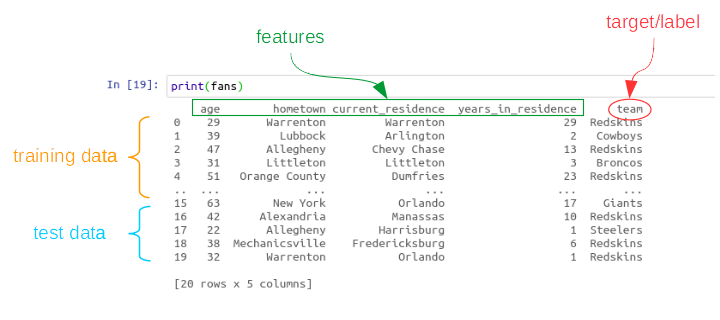
\includegraphics[width=1.05\textwidth]{footballML.png}
}}
\smallskip
\caption{Some labeled examples, divided into training and test sets.}
\label{fig:labeledTrainTest}
\end{figure}

\index{training data}
\index{test data}

You'll also see in the figure that I've split the rows up into two groups. The
first group is called the \textbf{training data}, and the second, the
\textbf{test data}. (Normally we'll shuffle all the rows before assigning them,
so that we don't put all the top rows of the \texttt{DataFrame} in the training
set and all the bottom ones in the test set. But that's harder to show in a
picture.)

\section{Three kinds of examples}

Now here's the deal. There are \textit{three} kinds of example rows we're going
to deal with:

\begin{compactenum}
\item \textbf{training data} -- \textit{labeled} examples which we will show to
our classifier, and from which it will try to find useful patterns to make
future predictions.
\item \textbf{test data} -- \textit{labeled} examples which we will
\textit{not} show to
our classifier, but which we will use to measure how well it performs.
\item \textbf{new data} -- \textit{unlabeled} examples that we will get in the
future, after we've deployed our classifier in the field, and which we will
feed to our classifier to make predictions.
\end{compactenum}

The purpose of the first group is to give the classifier useful information so
it can intelligently classify.

The purpose of the second group is \textit{to assess how good the classifier's
predictions are.} Since the test set consists of labeled examples, we know the
``true answer'' for each one. So we can feed each of these test points to the
classifier, look at its prediction, compare it to the true answer, and judge
whether or not the classifier got it right. Assessing its accuracy is usually
just a matter of computing the percentage of how many test points it got right.

The third group exists because after we've built and evaluated our classifier,
we actually want to put it into action! These are new data points (new sporting
goods customers, say) for which we don't know the ``true answer'' but want to
predict it so we can send catalogs likely to be well-received.

\subsection{Thou shalt not reuse}

\label{cantTestOnTrainingData}

Now one common question -- which leads to a \textit{super} important point --
is this: why can't we use \textit{all} the labeled examples as training data?
After all, if we have 1000 labeled examples we've had to work hard (or pay
\$\$) to get, it seems silly to only use some of them to train our classifier.
Shouldn't we want to give it all the labeled data possible, so it can learn the
maximum amount before predicting?

The first reply is: ``but then we wouldn't have any test data, and so we
wouldn't know how good our classifier \textit{was} before putting it out in the
field.'' Clearly, before we base major business decisions on the results of our
automated predictor, we need to have some idea of how accurate its predictions
are.

It's then commonly countered: ``well, sure, but why not then re-use those data
points for testing? Instead of splitting the 1000 examples into training points
and test points, why not just use all 1000 for training, and then test the
classifier on all 1000 points? What's not to like?''

This is where the super important point comes in, and it's so important that
I'll put it all in boldface. It turns out that \textbf{you absolutely
\textit{cannot} test your classifier on data points that you gave it to train
on, because you will get an overly optimistic estimate of how good your
classifier actually is.}

Here's an analogy to make this point more clear. Suppose there's a final exam
coming up in your class, and your professor distributes a ``sample exam'' a
week before exam day for you to study from. This is a reasonable thing to do.
As long as the questions on the sample exam are of the same type and difficulty
as the ones that will appear on the actual final, you'll learn lots about what
the professor expects you to know from taking the sample exam. And you'll
probably increase your actual exam score, since this will help you master
exactly the right material.

But suppose the professor uses the \textit{exact same} exam for both the sample
exam and the actual final exam? Sure, the students would be ecstatic, but
that's not the point. The point is: \textit{in this case, students wouldn't
even have to learn the material.} They could simply memorize the answers! And
after they all get their A's back, they might be tempted to think they're
really great at chemistry...but they probably aren't. They're probably just
really great at memorizing and regurgitating.

Going from ``the kinds of questions you may be asked'' to ``\textit{exactly}
the questions you \textit{will} be asked'' makes all the difference. And if you
just studied the sample exam by memorization, and were then asked (surprise!)
to demonstrate your understanding of the material on a \textit{new} exam, you'd
probably suck it up.

\index{generalizing (to new data)}

And so, the absolute iron-clad rule is this: \textbf{any data that is given to
the classifier to learn from must \textit{not} be used to test it.} The test
data must be comprised of representative, but different, examples. It's the
only way to assess how well the classifier \textbf{generalizes} to new data
that it hasn't yet seen (which, of course, is the whole point).


\subsection{Splitting the difference}

Okay, so given that we have to split our precious labeled examples into two
sets, one for training and one for testing, how much do we devote to each? It
turns out that there are some sophisticated techniques (beyond the scope of
this book, but stay tuned for Volume II) in which we can cleverly re-use
portions of the data for different purposes, and effectively make use of nearly
all of it for training.

\index{rule of thumb (for training/test data)}
But for our introductory approach here, we'll just use a \textbf{rule of thumb:
70\% for training data, and the other 30\% for test data}.

\index{shuffle (\texttt{DataFrame} rows)}
\index{randomization!of training and test data}
As I mentioned earlier, we'll normally \textbf{shuffle} the rows randomly
before dividing them into these two groups, just in case there's any pattern to
the order in which they appear. For example, in our NFL fan data set, it might
turn out that the data came to us sequenced in a way such that people living on
the east coast were at the beginning of the \texttt{DataFrame} and those living
out west were at the end. Any arrangement like this would spell doom for our
classification endeavor. For one thing, we wouldn't be training on any west
coast people, and so our classifier would be oblivious to what those data
points looked like. For another thing, we'd \textit{only} be using west
coasters to \textit{test} our classifier, meaning that whatever accuracy
measure we computed is likely to be way off. \textbf{Randomizing} the data is
the sure way around this.

\index{sample@\texttt{.sample()} (Pandas)}
\label{sampleRows}

Here's some code to create training and test sets. The \texttt{.sample()}
method of a \texttt{DataFrame} lets you choose some percentage of its rows 
randomly. Its \texttt{frac} argument is a number between 0 and 1 and specifies
what fraction of the rows you want. Using the above rule of thumb, let's choose
70\% of them for our training data:

\begin{Verbatim}[fontsize=\small,samepage=true,frame=single,framesep=3mm]
training = fans.sample(frac=.7)
print(training)
\end{Verbatim}
\vspace{-.2in}

\begin{Verbatim}[fontsize=\small,samepage=true,frame=leftline,framesep=5mm,framerule=1mm]
    age        hometown current_residence  years_in_residence      team
8    52       Arlington    Fredericksburg                  17  Redskins
15   63        New York           Orlando                  17    Giants
11   29  Fredericksburg           Seattle                  21  Seahawks
19   32       Warrenton           Orlando                   1  Redskins
2    47       Allegheny       Chevy Chase                  13  Redskins
7    31       Warrenton   Charlottesville                   6      Jets
0    29       Warrenton         Warrenton                  29  Redskins
5    32       Warrenton        Winchester                  11  Redskins
4    51   Orange County          Dumfries                  23  Redskins
9    60  Tyson's Corner      Falls Church                   4   Cowboys
10   17  Fredericksburg    Fredericksburg                  17  Redskins
1    39         Lubbock         Arlington                   2   Cowboys
13   35  Mechanicsville           Orlando                   8  Redskins
6    39        Dumfries             Miami                   5  Redskins
\end{Verbatim}

Notice that the numeric index values (far left) are in no particular order,
since that's the point of taking a random sample. Also notice that there are
only 14 rows in this \texttt{DataFrame} instead of the full 20 that were in
\texttt{fans}.

\index{not (query condition)}
\index{squiggle (tilde, or ``\texttt{\textasciitilde}'')}
\index{~@\texttt{\textasciitilde} (squiggle)}
\index{query}
\index{index@\texttt{.index} (little \texttt{i}) syntax}

Now, we want our test set. The trick here is to say: ``give me all the rows of
\texttt{fans} that were \textit{not} selected for the \texttt{training} set.''
By building a query with the squiggle operator (``\texttt{\textasciitilde}'',
meaning ``not'') in conjunction with the ``\texttt{.isin()}'' method, we can
create a new \texttt{DataFrame} called ``\texttt{test}'' that has exactly these
rows:

\begin{Verbatim}[fontsize=\small,samepage=true,frame=single,framesep=3mm]
test = fans[~fans.index.isin(training.index)]
print(test)
\end{Verbatim}
\vspace{-.2in}

\begin{Verbatim}[fontsize=\small,samepage=true,frame=leftline,framesep=5mm,framerule=1mm]
    age        hometown current_residence  years_in_residence      team
3    31       Littleton         Littleton                   3   Broncos
12   37        Richmond          Richmond                  37  Redskins
14   19        New York          New York                  19    Giants
16   42      Alexandria          Manassas                  10  Redskins
17   22       Allegheny        Harrisburg                   1  Steelers
18   38  Mechanicsville    Fredericksburg                   6  Redskins
\end{Verbatim}

That code says, in English: ``create a new variable \texttt{test} that contains
only those rows of \texttt{fans} whose index is \textit{not} present in any of
the \texttt{training} \texttt{DataFrame}'s indices.'' As you can verify through
visual inspection, the result does have exactly the 6 rows that were missing
from \texttt{training}.

\section{``The prior''}

\label{prior}
\index{prior@``the prior''}

One more piece of lingo before we dive into a particular classification
technique next chapter. And that's known as ``the \textbf{prior}'' of a data
set.

\index{Bayesian reasoning}
\index{posterior@posterior}

The term comes from something called \textbf{Bayesian reasoning}, which is a
whole subject (and a super cool one!) in its own right. All you need to know
here is the concept of two different quantities: the \textbf{prior}, and the
\textbf{posterior}.

In common usage, the word ``prior'' means ``beforehand,'' and so it does here:
the prior is your best judgment about what the target value of a new example
might be \textit{before you actually look at the feature values in that
example.} ``Posterior,'' on the other hand, means ``afterwards,'' and means
your best judgment about the target value after duly taking into consideration
all the feature values.

For example, you may have noticed that in my made-up data set, above, I had a
lot of Redskins fans. This is because I live in the D.C.~area, and happen to
know a lot of Redskins fans. Out of my 20 labeled examples, a whopping twelve
of them, in fact, had \texttt{Redskins} as their value in the \texttt{team}
column.

Thus, consider the following question. Suppose you knew nothing about a person
except that they were one of Stephen's friends. Which NFL team do you think
they'd support? Assuming this data set is representative of Stephen's friends,
you'd say: ``I'd predict they'd be a Redskins fan, and I'd estimate that I'd
have about a 60\% chance of being right ($\frac{12}{20}$).'' This is the
\textit{prior}. You're not taking into account anything about their age, where
they were born, \textit{etc.}; in fact, you weren't even told those things.
Instead, you're just ``using the prior'' and treating everyone the same.

It would be a different story if I told you that this person was born in New
York City. Then you might squint your eyes at my data set and realize that
there are only two New Yorkers in it, and neither one is a Redskins fan:
they're both Giants fans! Now you might very well move away from your prior
assumption. ``Sure, most of Stephen's friends are Redskins fans, so `Redskins'
is a reasonable guess, but now that you've told me they're from NY, that very
well might change my mind. Now, my guess is `Giants'.''

I keep saying ``might'' and ``may'' because different kinds of classifiers work
in different ways. Some of them may choose to take advantage of some features
but not others; some may just stick with the prior in certain situations. The
notion of ``the prior'' is mainly useful as a baseline for comparison: it's the
best you can do given no other possibly correlating information. The name of
the game in classification, of course, is to intelligently \textit{use} that
other information to make more informed guesses, and to beat the prior. One of
many ways to approach this is the decision tree classification algorithm, which
we'll look at in detail next.

% TODO: end this chapter with some brainstorming about how to create
% classifiers:
% 1. Flip a coin.
% 2. Just go with the prior.
% 3. Look up exactly the data point we're trying to classify (1-nn.)


\chapter{Decision trees for classification}

%So far this picture has been very general. We haven't said anything about
%
%
%I love the word ``training'' for this, by the way.


\chapter[Decision trees for classification (2 of 2)]{\huge\selectfont{Decision
trees for classification (2 of 2)}}
\label{ch:decisionTrees2}

\section{Decision Trees in Python}

\index{nested if statements@nested \texttt{if} statements}
\index{indentation}

Our decision tree pictures from chapter~\ref{ch:decisionTrees1} were quite
illustrative, but of course to actually automate something, we have to write
code rather than draw pictures. What would Figure~\ref{fig:decisionTree}
(p.~\pageref{fig:decisionTree}) look like in Python code? It's actually pretty
simple, although there's a lot of nested indentation. See if you can follow the
flow in Figure~\ref{fig:pythonDT}.

\begin{figure}[h]
\centering
\begin{Verbatim}[fontsize=\scriptsize,samepage=true,frame=single,framesep=3mm,xleftmargin=2cm,xrightmargin=2cm]
def predict(major, age, gender):
    if major == 'PSYC':
        return 'No'
    elif major == 'MATH':
        if gender == 'M':
            return 'No'
        elif gender == 'F' or gender == 'O':
            return 'Yes'
    elif major == 'CPSC':
        if age == 'young':
            return 'Yes'
        elif age == 'middle':
            return 'No'
        elif age == 'old':
            if gender == 'M' or gender == 'O':
                return 'Yes'
            elif gender == 'F':
                return 'No'
\end{Verbatim}
\caption{A Python implementation of the decision tree in
Figure~\ref{fig:decisionTree}.}
\label{fig:pythonDT}
\end{figure}

\index{predict@\texttt{predict()}}

Here we're defining a function called \texttt{predict()} that takes three
arguments, one for each feature value. The eye-popping set of
\texttt{if}/\texttt{elif}/\texttt{else} statements looks daunting at first, but
when you scrutinize it you'll realize it perfectly reflects the structure of
the purple diagram. Each time we go down one level of the tree, we indent one
tab to the right. The body of the ``\texttt{if major == \textquotesingle
PSYC\textquotesingle :}'' statement is very short because the left-most branch
of the tree (for Psychology) is very simple. The ``\texttt{elif major ==
\textquotesingle CPSC\textquotesingle :}'' body, by contrast, has lots of
nested internal structure precisely because the right-most branch of the tree
(for Computer Science) is complex. \textit{Etc.}

\begin{samepage}
If we call this function, it will give us exactly the same predictions we
calculated by hand on p.~\pageref{decisionTreeExamples}:

\begin{Verbatim}[fontsize=\footnotesize,samepage=true,frame=single,framesep=3mm]
print(predict('PSYC','M','old'))
print(predict('MATH','O','young'))
print(predict('CPSC','F','old'))
\end{Verbatim}
\vspace{-.2in}

\begin{Verbatim}[fontsize=\footnotesize,samepage=true,frame=leftline,framesep=5mm,framerule=1mm]
No
Yes
No
\end{Verbatim}
\end{samepage}

\section{Decision Tree induction}

Okay, so now we understand what a decision tree is, and even how to code one up
in Python. The key question that remains is: how do we figure out what tree to
build?

There are lots of different choices, even for our little videogame example. We
could put any of the three features at the root. For each branch from the root,
we could put either of the other features, or we could stop with a leaf. And
the leaf could be a \texttt{Yes} leaf or a \texttt{No} leaf. That's a lot of
``coulds.'' How can we know what a \textit{good} tree might be --
\textit{i.e.}, a tree that classifies new points more or less correctly?

\index{training data}
\index{inductive reasoning}

The answer, of course, is to take advantage of the training data. It consists
of labeled examples that are supposed to be our guide. Using the training data
to ``learn'' a good tree is called \textbf{inducing} a decision tree. Let's see
how.

\subsection{``Greedy'' algorithms}

\index{greedy (algorithm)}

Our decision tree induction algorithm is going to be a \textbf{greedy} one.
This means that instead of looking ahead and strategizing about future nodes
far down on the tree, we're just going to grab the immediate best-looking
feature at every individual step and use that. This won't by any means
guarantee us the best possible tree, but it will be quick to learn one.

\index{chess}

An illustration to help you understand greedy algorithms is to think about a
strategy game like chess. If you've ever played chess, you know that the only
way to play well is to think ahead several moves, and anticipate your
opponent's probable responses. You can't just look at the board na\"{i}vely and
say, ``why look at that: if I move my rook up four squares, I'll capture my
opponent's pawn! Let's do it!'' Without considering the broader implications of
your move, you're likely to discover that as soon as you take her pawn, she
turns around and takes your rook because she's lured you into a trap.

A \textit{greedy} algorithm for chess would do exactly that, however. It would
just grab whatever morsel was in front of it without considering the fuller
consequences. That may seem really dumb -- and it is, for chess -- but for
certain other problems it turns out to be a decent approach. And decision tree
induction is one of those.

The reason we resort to a greedy algorithm is that for any real-sized data set,
\textit{the number of possible trees to consider is absolutely overwhelming.}
There's simply not enough time left in the universe to look at them all -- and
that's not an exaggeration. So you have to find \textit{some} way of picking a
tree without actually contemplating every one, and it turns out that grabbing
the immediately best-looking feature at each level is a pretty good way to do
that.

\subsection{Choosing ``the immediate best'' feature}

Now what does that mean, anyway: ``choosing the immediate best feature?'' We're
going to define it as follows: the best feature to put at any given node is
\textit{the one which, if we did no further branching from that node but
instead put only leaves below it, would classify the most training points
correctly.} Let's see how this works for the videogame example.

\index{value\_counts@\texttt{.value\_counts()} method (Pandas)}
\index{groupby@\texttt{.groupby()} method (Pandas)}

Our left-most feature in the \texttt{DataFrame} is \textsf{Major}, so let's
consider that one first. Suppose we put \textsf{Major} at the root of the tree,
and then made each of its branches lead to leaves. What value should we predict
for each of the majors? Well, we can answer that with another clever use of
\texttt{.value\_counts()}, this time conjoining it with a call to
\texttt{.groupby()}. Check out this primo line of code:

\begin{Verbatim}[fontsize=\small,samepage=true,frame=single,framesep=3mm]
students.groupby('Major').VG.value_counts()
\end{Verbatim}

Stare hard at that code. You'll realize that all these pieces are things you
already know: we're just combining them in new ways. That line of code says
``take the entire \texttt{students} \texttt{DataFrame}, but treat each of the
majors as a separate group. And what should we do with each group? Well, we
count up the values of the \texttt{VG} column for the rows in that group.'' The
result is as follows:

\begin{Verbatim}[fontsize=\small,samepage=true,frame=leftline,framesep=5mm,framerule=1mm]
Major  VG 
PSYC   No     3
       Yes    2
MATH   No     3
       Yes    1
CPSC   No     4
       Yes    4
Name: VG, dtype: int64
\end{Verbatim}

We can answer ``how many would we get right?'' by reading right off that chart.
For the \texttt{PSYC} majors, there are two who play videogames and three who
do not. Clearly, then, if we presented a Psychology major to this decision
tree, it ought to predict '\texttt{No}', and that prediction would be correct
for 3 out of the 5 Psychology majors on record. For the \texttt{MATH} majors,
we would again predict '\texttt{No}', and we'd be correct 3 out of \textit{4}
times. Finally, for the \texttt{CPSC} majors, we have 4 \texttt{Yes}es and 4
\texttt{No}s, so that's not much help. We essentially have to pick randomly
since the training data doesn't guide us to one answer or the other. Let's
choose '\texttt{Yes}' for our Computer Science answer, just so it's different
than the others. The best one-level decision tree that would result from
putting \textsf{Major} at the top is therefore depicted in
Figure~\ref{fig:majorOnTop}. It gets \textbf{ten} out of the seventeen training
points correct (59\%). Your reaction is probably ``Big whoop -- we got that
good a score just using the prior, and ignoring all the features!'' Truth.
Don't lose hope, though: \textsf{Major} was only one of our three choices.

\begin{figure}[ht]
\centering
\includegraphics[width=0.6\textwidth]{majorOnTop.png}
\caption{A one-level decision tree if we put the \textsf{Major} feature at the
root -- it would classify \textbf{ten} of the seventeen training points
correctly.}
\label{fig:majorOnTop}
\end{figure}

Let's repeat this analysis for the other two features and see if either one
fares any better. Here's the query for \textsf{Age}:

\begin{Verbatim}[fontsize=\small,samepage=true,frame=single,framesep=3mm]
students.groupby('Age').VG.value_counts()
\end{Verbatim}

This yields:

\begin{Verbatim}[fontsize=\small,samepage=true,frame=leftline,framesep=5mm,framerule=1mm]
Age     VG 
middle  No     6
        Yes    2
old     Yes    2
        No     1
young   No     3
        Yes    3
Name: VG, dtype: int64
\end{Verbatim}

Making the sensible predictions at the leaves based on these values gives the
tree in Figure~\ref{fig:ageOnTop}. It gets \textbf{eleven} points right (65\%)
-- a bit of an improvement.

\begin{figure}[ht]
\centering
\includegraphics[width=0.6\textwidth]{ageOnTop.png}
\caption{A one-level decision tree if we chose the \textsf{Age} feature for the
root -- it would classify \textbf{eleven} of the seventeen training points
correctly.}
\label{fig:ageOnTop}
\end{figure}

Finally, we could put \textsf{Gender} at the root. Here's the query for it:

\begin{samepage}
\begin{Verbatim}[fontsize=\small,samepage=true,frame=single,framesep=3mm]
students.groupby('Gender').VG.value_counts()
\end{Verbatim}
\vspace{-.2in}

\begin{Verbatim}[fontsize=\small,samepage=true,frame=leftline,framesep=5mm,framerule=1mm]
Gender  VG 
F       No     8
        Yes    2
M       Yes    5
        No     1
O       No     1
Name: VG, dtype: int64
\end{Verbatim}
\end{samepage}

Paydirt! Splitting on the \textsf{Gender} feature first, as shown in
Figure~\ref{fig:genderOnTop}, gets us a whopping \textbf{fourteen} points
correct, or over 82\%. This is clearly the winner of the three. And since we're
being greedy and not bothering to look further downstream anyway, we hereby
elect to put \textsf{Gender} at the root of our tree.

\begin{figure}[ht]
\centering
\includegraphics[width=0.6\textwidth]{genderOnTop.png}
\caption{A one-level decision tree if we chose the \textsf{Gender} feature for
the root. It would classify \textbf{fourteen} of the seventeen training points
correctly -- easily the best of the three choices.}
\label{fig:genderOnTop}
\end{figure}

It's worth taking a moment to look at those \texttt{.value\_counts()} outputs
and see if you can develop some intuition about why \textsf{Gender} worked so
much better at the root than the other two features did. The reason is that for
this data set, \textsf{Gender} split the data into groups that were more
\textbf{homogeneous} than the other splits gave. ``Homogeneous'' here means
that each group was more ``pure,'' or put another way, more lopsided towards
one of the labels. \textsf{Gender} gave us a 5-to-1 lopsided ratio on the
\texttt{M} branch, and an even more lopsided 2-to-8 ratio on the \texttt{F}
branch. Intuitively, this means that \textsf{Gender} really is correlated with
videogame use, and this shows up in purer splits. Contrast this with the
situation when we split on \textsf{Major} first, and we ended up with a yucky
4-to-4 ratio on the \texttt{CPSC} branch. An even split is the worst of all
possible worlds: here, it means that learning someone's a Computer Science
major doesn't tell you jack about their videogame use. That in turn means it's
pretty useless to split on.

\subsection{Lather, rinse, repeat}

\index{turtle}

So far, we've done all that work just to figure out which feature to put at the
root of our tree. Now, we progress down each of the branches and do the exact
same thing: figure out what to put at each branch. We'll continue on and on
like this for the entire tree. It's turtles all the way down.

% To keep this chapter at least somewhat brief, we'll do just one more layer of
% the tree.

Let's consider the \textit{left} branch of Figure~\ref{fig:genderOnTop}. What
do we do with males? There are now only two remaining features to split on. (It
wouldn't make sense to split on \textsf{Gender} again, since the only people
who will reach the left branch are males anyway: there'd be nothing to split
on.)

Thus we could put either \textsf{Major} or \textsf{Age} at that left branch. To
figure out which one is better, we'll do the same thing we did before, only
with one slight change: now, we need to consider \textit{only males} in our
analysis.

We augment our primo line of code from above with a query at the beginning, so
that our counts include only males:

\begin{Verbatim}[fontsize=\small,samepage=true,frame=single,framesep=3mm]
students[students.Gender=="M"].groupby('Major').VG.value_counts()
\end{Verbatim}
\vspace{-.2in}

\begin{Verbatim}[fontsize=\small,samepage=true,frame=leftline,framesep=5mm,framerule=1mm]
Major  VG 
CPSC   Yes    3
MATH   No     1
       Yes    1
PSYC   Yes    1
Name: VG, dtype: int64
\end{Verbatim}

Wow, cool: the \texttt{CPSC} and \texttt{PSYC} folks are perfectly homogeneous
now. If we end up deciding to split on \textsf{Major} here, we can put
permanent dark purple squares for each of those majors simply declaring
``Yes.'' In all, splitting here gives us 5 out of 6 correct. The
tree-in-progress we'd end up with is in Figure~\ref{fig:maleMajorSplit}.

\begin{figure}[ht]
\centering
\includegraphics[width=0.7\textwidth]{maleMajorSplit.png}
\caption{The tree-in-progress if we choose to split on \textsf{Major} in the
male branch.}
\label{fig:maleMajorSplit}
\end{figure}

\begin{samepage}
Our other choice, of course, is to split on \textsf{Age} instead:

\begin{Verbatim}[fontsize=\small,samepage=true,frame=single,framesep=3mm]
students[students.Gender=="M"].groupby('Age').VG.value_counts()
\end{Verbatim}
\vspace{-.2in}
\end{samepage}

\begin{Verbatim}[fontsize=\small,samepage=true,frame=leftline,framesep=5mm,framerule=1mm]
Age     VG 
middle  No     1
        Yes    1
old     Yes    1
young   Yes    3
Name: VG, dtype: int64
\end{Verbatim}

Again, 5 out of 6 correct. Here, \texttt{middle}-aged students are the only
heterogeneous group; the \texttt{old} folks and \texttt{young}-uns are clean
splits. With this choice, our tree would appear as in
Figure~\ref{fig:maleAgeSplit}.

\begin{figure}[ht]
\centering
\includegraphics[width=0.7\textwidth]{maleAgeSplit.png}
\caption{On the other hand, the tree-in-progress if we choose to split on
\textsf{Age} in the male branch instead.}
\label{fig:maleAgeSplit}
\end{figure}

So at this point, since splitting on either feature and then stopping would
give us exactly 5 out of 6 points correct, we just flip a coin. I just flipped
one, and it came out tails (for \textsf{Age}) -- hope that's okay with you.

\subsubsection{Finishing up the left branch}

The two ``Yes'' leaves in Figure~\ref{fig:maleAgeSplit} are now set in stone,
since every single \texttt{young} male in our training set was indeed a
videogamer, as was every \texttt{old} male. Now we just have to deal with the
\texttt{middle} branch.

Only one feature now remains to split on -- \textsf{Major} -- so we'll do that,
and produce the result in Figure~\ref{fig:maleAgeMiddle}. There's exactly one
\texttt{middle}-aged male \texttt{MATH} major in the original
\texttt{DataFrame} (line 12, p.~\pageref{vgDataSet}), and he's labeled ``No,''
so we'll guess ``No'' in the \texttt{MATH} branch. Similarly, we have one data
point to guide us for \texttt{CPSC} majors (line 3), so we'll predict ``Yes''
in this case. The \texttt{PSYC} branch presents a conundrum, though: our data
set doesn't have \textit{any} \texttt{middle}-aged male Psychology majors, so
how do we know what to guess in this case?

\begin{figure}[ht]
\centering
\includegraphics[width=0.8\textwidth]{maleAgeMiddle.png}
\caption{Going one level further down after splitting on \textsf{Age} for
males. We have data for \texttt{middle}-aged \texttt{CPSC} and \texttt{MATH}
males...but what to do with \texttt{middle}-aged \texttt{PSYC} males?}
\label{fig:maleAgeMiddle}
\end{figure}

The best way to handle this is to fall back to a more general case where you
\textit{do} have examples. It's true that we have no training points for
\texttt{middle}-aged male Psychology majors, but we \textit{do} have points for
\texttt{middle}-aged males-in-general, and we discovered that 5 out of 6 of
them were gamers. So it makes sense to default to ``Yes'' in the \texttt{PSYC}
branch of this part of the tree, even though we don't have any data points
exactly like that. So that's what we'll do. The finished left branch is
depicted in Figure~\ref{fig:maleAgeMiddleWithPsyc}.

\begin{figure}[ht]
\centering
\includegraphics[width=0.7\textwidth]{maleAgeMiddleWithPsyc.png}
\caption{The decision tree we're in the process of inducing, with the left
branch entirely completed.}
\label{fig:maleAgeMiddleWithPsyc}
\end{figure}

\subsubsection{Finishing up the rest of the tree}

The rest of the process is just the same stuff done over and over.\footnote{If
you're wondering whether there's a way to automate this, the answer is a
resounding \textbf{yes}! There are many packages in Python and other languages
which will automatically build a decision tree from a training set; the
\texttt{DecisionTreeClassifier} from the \texttt{scikit-learn} package is one
of them. This exercise of learning how to build a decision tree manually is so
you can understand the concepts of what's going on under the hood -- kind of
like you learn how to add numbers in grade school even though you'll normally
use a calculator later on in life.} At each branch of the tree, we take the
subset of the training points that remain (\textit{i.e.}, the training points
that match the path from the root thus far, and are therefore applicable), and
decide what to branch on next. When we get to a completely homogeneous group,
we stop and put a leaf there. The end result of all these efforts is the final
decision tree for the videogame data set, in Figure~\ref{fig:completeVgTree},
and its Python equivalent in Figure~\ref{fig:completeVgTreePython}.

\index{contradiction (in a training set)}

One interesting aspect of our final tree is the
female$\rightarrow$\texttt{PSYC}$\rightarrow$\texttt{middle}-aged branch.
You'll see that this leaf is labeled ``Yes(?)'' in the diagram. Why the
question mark? Because this is the one case where we have a
\textbf{contradiction} in our training data. Check out lines 2 and 16 back on
p.~\pageref{vgDataSet}. They each reflect a \texttt{middle}-aged female
Psychology major, but with \textit{different} labels: the first one is not a
videogame player, but the second one is.

I always thought the term ``contradiction'' was amusing here. Two similar
people don't have exactly the same hobbies -- so what? Is that really so
surprising? Do all middle-aged female Psychology majors have to be identical?

Of course not. But you can also see things from the decision tree's point of
view. The \textit{only} things it knows about people are those three
attributes, and so as far as the decision tree is concerned, the people on
lines 2 and 16 really \textit{are} indistinguishable. When contradictions
occur, we have no choice but to fall back on some sort of majority-rules
strategy: if out of seven otherwise-identical people, two play videogames and
five do not, we'd predict ``No'' in that branch. In the present case, we can't
even do \textit{that} much, because we have exactly one of each. So I'll just
flip a coin again. (\texttt{*flip*}) It came up heads, so we'll go with
``Yes.''

Notice that in this situation, the resulting tree will actually misclassify one
or more \textit{training} points. If we called our function in
Figure~\ref{fig:completeVgTreePython} and passed it our person from line 2
(\texttt{\textquotesingle PSYC\textquotesingle}, \texttt{\textquotesingle
middle\textquotesingle}, \texttt{\textquotesingle F\textquotesingle}), it would
return \texttt{"Yes"} even though line 2 is not a gamer. Furthermore,
contradictions are the \textit{only} situation in which this will ever happen;
if the data is contradiction-free, then every training point will be classified
correctly by the decision tree.

Paradoxically, it turns out that's not necessarily a good thing, as we'll
discover in Volume II of this series. For now, though, we'll simply declare
victory.

\begin{figure}[ht]
\centering
\includegraphics[width=1\textwidth]{completeVgTree.png}
\caption{The final decision tree for the videogame data set.}
\label{fig:completeVgTree}
\end{figure}

\begin{figure}[ht]
\centering
\begin{Verbatim}[fontsize=\scriptsize,samepage=true,frame=single,framesep=3mm,xleftmargin=2cm,xrightmargin=2cm]
def predict(major, age, gender):
    if gender == 'M':
        if age == 'young':
            return 'Yes'
        elif age == 'middle':
            if major == 'PSYC' or major == 'CPSC':
                return 'Yes'
            elif major == 'MATH':
                return 'No'
        elif age == 'old':
            return 'Yes'
    elif gender == 'F':
        if major == 'MATH':
            return 'No'
        elif major == 'CPSC':
            if age == 'young' or age == 'middle':
                return 'No'
            elif age == 'old':
                return 'Yes'
        elif major == 'PSYC':
            if age == 'young' or age == 'old':
                return 'No'
            elif age == 'middle':
                return 'Yes'  # Here's our "contradiction"
    elif gender == 'O':
        return 'No'
\end{Verbatim}
\caption{The final decision tree for the videogame data set, as a Python
function.}
\label{fig:completeVgTreePython}
\end{figure}

% split a numerical attribute into categorical


\chapter{Evaluating a classifier}



% Add empty page to get to a multiple of 12 (306 total pages).
\begingroup
  \null
  \newpage
\endgroup
\backmatter
\printindex

% Add empty (number-less) pages to get to a multiple of 12 (306 total pages).
\shipout\null
\shipout\null
\shipout\null
\shipout\null

\end{document}
